%Page Setup, don't remove
\documentclass[12pt]{book} 
\setlength{\columnsep}{0.7truecm}
\setlength{\parindent}{0cm}
\usepackage[top=2truecm,bottom=2.8truecm, left=2.2truecm, right=2.2truecm,headsep=10pt, paperwidth=19.3truecm, paperheight=27.6truecm]{geometry} 
\usepackage[usenames,dvipsnames]{xcolor}
\usepackage{tcolorbox}
\definecolor{ocre}{RGB}{52,177,201} 
\usepackage{pdfpages}
\usepackage{avant}
\usepackage{bussproofs}
\usepackage{mathptmx}
%\usepackage{ebgaramond}
 \usepackage{xeCJK}
 \setCJKmainfont{SimSun}
\usepackage{tikz}
\usepackage{tkz-euclide}
\usepackage{matchsticks}
\usepackage{wrapfig}
\usepackage{listings}
\usepackage[utf8]{vietnam}
\usepackage{babel}
\usepackage[LSBC5,T1]{fontenc}

%----------------------------------------------------------------------------------------
%	VARIOUS REQUIRED PACKAGES
%----------------------------------------------------------------------------------------
\usepackage{titlesec} % Allows customization of titles
\usepackage{multicol}
\usepackage{graphicx} % Required for including pictures
%\graphicspath{{Pictures/}} % Specifies the directory where pictures are stored
\usepackage{lipsum} % Inserts dummy text
\usepackage{tikz} % Required for drawing custom shapes
%\usepackage{enumitem} % Customize lists
%\setlist{nolistsep} % Reduce spacing between bullet points and numbered lists
\usepackage{booktabs} % Required for nicer horizontal rules in tables
\usepackage{eso-pic} % Required for specifying an image background in the title page
\usepackage{titletoc} % Required for manipulating the table of contents
\contentsmargin{0cm} % Removes the default margin
\usepackage{adjustbox} 
\usepackage{amsmath,amsfonts,amssymb,amsthm} % For math equations, theorems, symbols, etc
%\usepackage[framemethod=tikz]{mdframed} 
\usepackage[sexy]{evan}
\usepackage{hyperref}
\urlstyle{same}
\usepackage{tikz} % figure in two column
\usepackage{float}
\usepackage{biblatex}
\usepackage{caption}% dinh dang figure caption
%\usepackage[font=normalsize]{caption}
\usepackage{changepage}
\usepackage{booktabs}

\usepackage{chngcntr}
\usepackage{array}
\usepackage{eurosym}
\usepackage{multirow}
\usepackage{mathtools}
\usepackage{setspace}
\usepackage{afterpage}
\usepackage{scalerel}
\usepackage{blindtext}
\usepackage{tabularx}
\usepackage{afterpage}
\usepackage{array}
%\usepackage{transparent}
\usepackage{efbox}
\usepackage{tabulary}
% \usepackage{CJKutf8}
\usepackage{subcaption}
\usepackage{rotating}
\usepackage{microtype}
\usepackage{pgfplots}

\usetikzlibrary{lindenmayersystems}
\usetikzlibrary{shapes,shapes.geometric}
\usetikzlibrary{decorations.pathreplacing}
\usetikzlibrary{calc,intersections}
\usetikzlibrary[shadings]
\usetikzlibrary{decorations.fractals}

\newmdenv[skipabove=7pt,
skipbelow=7pt,
backgroundcolor=black!5,
linecolor=ocre,
leftline=true,
innerleftmargin=6pt,
innerrightmargin=6pt,
innertopmargin=8pt,
leftmargin=0cm,
rightmargin=0cm,
innerbottommargin=8pt]{tBox}

\def\PIbox#1{\tikz\node[draw = ocre,fill=black!5,align=justify,text width=.95\linewidth,inner sep=2mm]{#1};}%
\renewcommand{\qedsymbol}{}	
\usepackage{fancyhdr} % Required for header and footer configuration
%%%% Header for duong vao toan hoc
\fancypagestyle{duongvaotoanhoc}{
	\fancyhf{}
	\fancyhead[E]{
		\insertpic{63}{740}{1}{duongvao1}
		\insertpic{333}{35}{1}{fduongvao1}
}
	\fancyhead[O]{
		\insertpic{1}{740}{1}{duongvao2}
		\insertpic{59}{34.9}{1}{fduongvao2}
}	
\renewcommand{\footrulewidth}{0pt}
\fancyfoot[LE,RO]{\sffamily\footnotesize	\thepage}

\fancyfoot[LO,RE]{\sffamily\scriptsize TẬP 7 -- SỐ 4 THÁNG 4/2023}
}

\fancypagestyle{duongvaotoanhocnone}{
	\fancyhf{}
	\fancyhead[E]{
		\insertpic{333}{35}{1}{fduongvao1}
	}
	\fancyhead[O]{
		\insertpic{59}{34.9}{1}{fduongvao2}
	}	
	\renewcommand{\footrulewidth}{0pt}
	\fancyfoot[LE,RO]{\sffamily\footnotesize	\thepage}
	
	\fancyfoot[LO,RE]{\sffamily\scriptsize TẬP 7 -- SỐ 4 THÁNG 4/2023}
}

\fancypagestyle{thachthuctoanhoc}{
	\fancyhf{}
	\fancyhead[E]{
		\insertpic{63}{740}{1}{thachthuc1}
		\insertpic{333}{35}{1}{fthachthuc1}
	}
	\fancyhead[O]{
		\insertpic{1}{740}{1}{thachthuc2}
		\insertpic{59}{34.9}{1}{fthachthuc2}
	}	
	\renewcommand{\footrulewidth}{0pt}
	\fancyfoot[LE,RO]{\sffamily\footnotesize	\thepage}
	
	\fancyfoot[LO,RE]{\sffamily\scriptsize TẬP 7 -- SỐ 4 THÁNG 4/2023}
}

\fancypagestyle{thachthuctoanhocnone}{
	\fancyhf{}
	\fancyhead[E]{
		\insertpic{333}{35}{1}{fthachthuc1}
	}
	\fancyhead[O]{
		\insertpic{59}{34.9}{1}{fthachthuc2}
	}	
	\renewcommand{\footrulewidth}{0pt}
	\fancyfoot[LE,RO]{\sffamily\footnotesize	\thepage}
	
	\fancyfoot[LO,RE]{\sffamily\scriptsize TẬP 7 -- SỐ 4 THÁNG 4/2023}
}


%%%% Header for Toán học và đời sống
\fancypagestyle{toanhocvadoisong}{
			\fancyhf{}
		\fancyhead[E]{
			\insertpic{63}{740}{1}{toanhocds1}
			\insertpic{333}{35}{1}{ftoanhocds1}
		}
		\fancyhead[O]{
			\insertpic{1}{740}{1}{toanhocds2}
			\insertpic{59}{34.9}{1}{ftoanhocds2}
		}	
		\renewcommand{\footrulewidth}{0pt}
		\fancyfoot[LE,RO]{\sffamily\footnotesize	\thepage}
		
		\fancyfoot[LO,RE]{\sffamily\scriptsize TẬP 7 -- SỐ 4 THÁNG 4/2023}
}
\fancypagestyle{toanhocvadoisongnone}{
	\fancyhf{}
	\fancyhead[E]{
		\insertpic{333}{35}{1}{ftoanhocds1}
	}
	\fancyhead[O]{
		\insertpic{59}{34.9}{1}{ftoanhocds2}
	}	
	\renewcommand{\footrulewidth}{0pt}
	\fancyfoot[LE,RO]{\sffamily\footnotesize	\thepage}
	
	\fancyfoot[LO,RE]{\sffamily\scriptsize TẬP 7 -- SỐ 4 THÁNG 4/2023}
}

\fancypagestyle{doisongtoanhoc}{
	\fancyhf{}
	\fancyhead[E]{
		\insertpic{63}{740}{1}{dstoanhoc1}
		\insertpic{333}{35}{1}{fdstoanhoc1}
	}
	\fancyhead[O]{
		\insertpic{1}{740}{1}{dstoanhoc2}
		\insertpic{59}{34.9}{1}{fdstoanhoc2}
	}	
	\renewcommand{\footrulewidth}{0pt}
	\fancyfoot[LE,RO]{\sffamily\footnotesize	\thepage}
	
	\fancyfoot[LO,RE]{\sffamily\scriptsize TẬP 7 -- SỐ 4 THÁNG 4/2023}
}
\fancypagestyle{doisongtoanhocnone}{
	\fancyhf{}
	\fancyhead[E]{
		\insertpic{333}{35}{1}{fdstoanhoc1}
	}
	\fancyhead[O]{
		\insertpic{59}{34.9}{1}{fdstoanhoc2}
	}	
	\renewcommand{\footrulewidth}{0pt}
	\fancyfoot[LE,RO]{\sffamily\footnotesize	\thepage}
	
	\fancyfoot[LO,RE]{\sffamily\scriptsize TẬP 7 -- SỐ 4 THÁNG 4/2023}
}

%%% doi thoai toan hoc
\fancypagestyle{doithoaitoanhoc}{
	\fancyhf{}
	\fancyhead[E]{
		\insertpic{63}{740}{1}{doithoai1}
		\insertpic{333}{35}{1}{fdoithoai1}
	}
	\fancyhead[O]{
		\insertpic{1}{740}{1}{doithoai2}
		\insertpic{59}{34.9}{1}{fdoithoai2}
	}	
	\renewcommand{\footrulewidth}{0pt}
	\fancyfoot[LE,RO]{\sffamily\footnotesize	\thepage}
	
	\fancyfoot[LO,RE]{\sffamily\scriptsize TẬP 7 -- SỐ 4 THÁNG 4/2023}
}
\fancypagestyle{doithoaitoanhocnone}{
	\fancyhf{}
	\fancyhead[E]{
		\insertpic{333}{35}{1}{fdoithoai1}
	}
	\fancyhead[O]{
		\insertpic{59}{34.9}{1}{fdoithoai2}
	}	
	\renewcommand{\footrulewidth}{0pt}
	\fancyfoot[LE,RO]{\sffamily\footnotesize	\thepage}
	
	\fancyfoot[LO,RE]{\sffamily\scriptsize TẬP 7 -- SỐ 4 THÁNG 4/2023}
}

%%%% Header for co dien hien dai
\fancypagestyle{codienhiendai}{
	\fancyhf{}
	\fancyhead[E]{
		\insertpic{63}{740}{1}{codien1}
		\insertpic{333}{35}{1}{fcodien1}
	}
	\fancyhead[O]{
		\insertpic{1}{740}{1}{codien2}
		\insertpic{59}{34.9}{1}{fcodien2}
	}	
	\renewcommand{\footrulewidth}{0pt}
	\fancyfoot[LE,RO]{\sffamily\footnotesize	\thepage}
	
	\fancyfoot[LO,RE]{\sffamily\scriptsize TẬP 7 -- SỐ 4 THÁNG 4/2023}
}
\fancypagestyle{codienhiendainone}{
	\fancyhf{}
	\fancyhead[E]{
		\insertpic{333}{35}{1}{fcodien1}
	}
	\fancyhead[O]{
		\insertpic{59}{34.9}{1}{fcodien2}
	}	
	\renewcommand{\footrulewidth}{0pt}
	\fancyfoot[LE,RO]{\sffamily\footnotesize	\thepage}
	
	\fancyfoot[LO,RE]{\sffamily\scriptsize TẬP 7 -- SỐ 4 THÁNG 4/2023}
}

\fancypagestyle{diendandayvahoctoan}{
	\fancyhf{}
	\fancyhead[E]{
		\insertpic{63}{740}{1}{diendan1}
		\insertpic{333}{35}{1}{fdiendan1}
	}
	\fancyhead[O]{
		\insertpic{1}{740}{1}{diendan2}
		\insertpic{59}{34.9}{1}{fdiendan2}
	}	
	\renewcommand{\footrulewidth}{0pt}
	\fancyfoot[LE,RO]{\sffamily\footnotesize	\thepage}
	
	\fancyfoot[LO,RE]{\sffamily\scriptsize TẬP 7 -- SỐ 4 THÁNG 4/2023}
}
\fancypagestyle{diendandayvahoctoannone}{
	\fancyhf{}
	\fancyhead[E]{
		\insertpic{333}{35}{1}{fdiendan1}
	}
	\fancyhead[O]{
		\insertpic{59}{34.9}{1}{fdiendan2}
	}	
	\renewcommand{\footrulewidth}{0pt}
	\fancyfoot[LE,RO]{\sffamily\footnotesize	\thepage}
	
	\fancyfoot[LO,RE]{\sffamily\scriptsize TẬP 7 -- SỐ 4 THÁNG 4/2023}
}

\fancypagestyle{cackithitoan}{
	\fancyhf{}
	\fancyhead[E]{
		\insertpic{63}{740}{1}{cackithi1}
		\insertpic{333}{35}{1}{fcackithi1}
	}
	\fancyhead[O]{
		\insertpic{1}{740}{1}{cackithi2}
		\insertpic{59}{34.9}{1}{fcackithi2}
	}	
	\renewcommand{\footrulewidth}{0pt}
	\fancyfoot[LE,RO]{\sffamily\footnotesize	\thepage}
	
	\fancyfoot[LO,RE]{\sffamily\scriptsize TẬP 7 -- SỐ 4 THÁNG 4/2023}
}
\fancypagestyle{cackithitoannone}{
	\fancyhf{}
	\fancyhead[E]{
		\insertpic{333}{35}{1}{fcackithi1}
	}
	\fancyhead[O]{
		\insertpic{59}{34.9}{1}{fcackithi2}
	}	
	\renewcommand{\footrulewidth}{0pt}
	\fancyfoot[LE,RO]{\sffamily\footnotesize	\thepage}
	
	\fancyfoot[LO,RE]{\sffamily\scriptsize TẬP 7 -- SỐ 4 THÁNG 4/2023}
}

\fancypagestyle{lichsutoanhoc}{
	\fancyhf{}
	\fancyhead[E]{
		\insertpic{63}{740}{1}{lichsu1}
		\insertpic{333}{35}{1}{flichsu1}
	}
	\fancyhead[O]{
		\insertpic{1}{740}{1}{lichsu2}
		\insertpic{59}{34.9}{1}{flichsu2}
	}	
	\renewcommand{\footrulewidth}{0pt}
	\fancyfoot[LE,RO]{\sffamily\footnotesize	\thepage}
	
	\fancyfoot[LO,RE]{\sffamily\scriptsize TẬP 7 -- SỐ 4 THÁNG 4/2023}
}
\fancypagestyle{lichsutoanhocnone}{
	\fancyhf{}
	\fancyhead[E]{
		\insertpic{333}{35}{1}{flichsu1}
	}
	\fancyhead[O]{
		\insertpic{59}{34.9}{1}{flichsu2}
	}	
	\renewcommand{\footrulewidth}{0pt}
	\fancyfoot[LE,RO]{\sffamily\footnotesize	\thepage}
	
	\fancyfoot[LO,RE]{\sffamily\scriptsize TẬP 7 -- SỐ 4 THÁNG 4/2023}
}

%%%% Header for Tìm hiểu khoa học
\fancypagestyle{timhieukhoahoc}{
		\fancyhf{}
	\fancyhead[E]{
		\insertpic{63}{740}{1}{timhieu1}
		\insertpic{333}{35}{1}{ftimhieu1}
	}
	\fancyhead[O]{
		\insertpic{1}{740}{1}{timhieu2}
		\insertpic{59}{34.9}{1}{ftimhieu2}
	}	
	\renewcommand{\footrulewidth}{0pt}
	\fancyfoot[LE,RO]{\sffamily\footnotesize	\thepage}
	
	\fancyfoot[LO,RE]{\sffamily\scriptsize TẬP 7 -- SỐ 4 THÁNG 4/2023}	
}
\fancypagestyle{timhieukhoahocnone}{
	\fancyhf{}
	\fancyhead[E]{
		\insertpic{333}{35}{1}{ftimhieu1}
	}
	\fancyhead[O]{
		\insertpic{59}{34.9}{1}{ftimhieu2}
	}	
	\renewcommand{\footrulewidth}{0pt}
	\fancyfoot[LE,RO]{\sffamily\footnotesize	\thepage}
	
	\fancyfoot[LO,RE]{\sffamily\scriptsize TẬP 7 -- SỐ 4 THÁNG 4/2023}	
}

%%%% Header for quan toan
\fancypagestyle{quantoan}{
		\fancyhf{}
		\fancyhead[E]{
		\insertpic{63}{740}{1}{quantoan1}
		\insertpic{333}{35}{1}{fquantoan1}
	}
	\fancyhead[O]{
		\insertpic{1}{740}{1}{quantoan2}
		\insertpic{59}{34.9}{1}{fquantoan2}
	}	
	\renewcommand{\footrulewidth}{0pt}
	\fancyfoot[LE,RO]{\sffamily\footnotesize	\thepage}
	
	\fancyfoot[LO,RE]{\sffamily\scriptsize TẬP 7 -- SỐ 4 THÁNG 4/2023}
}
\fancypagestyle{quantoannone}{
	\fancyhf{}
	\fancyhead[E]{
		\insertpic{333}{35}{1}{fquantoan1}
	}
	\fancyhead[O]{
		\insertpic{59}{34.9}{1}{fquantoan2}
	}	
	\renewcommand{\footrulewidth}{0pt}
	\fancyfoot[LE,RO]{\sffamily\footnotesize	\thepage}
	
	\fancyfoot[LO,RE]{\sffamily\scriptsize TẬP 7 -- SỐ 4 THÁNG 4/2023}
}


\fancypagestyle{hoccungpi}{
				\fancyhf{}
		\fancyhead[E]{
			\insertpic{63}{740}{1}{hoccungpi1}
			\insertpic{333}{35}{1}{fhoccungpi1}
		}
		\fancyhead[O]{
			\insertpic{1}{740}{1}{hoccungpi2}
			\insertpic{59}{34.9}{1}{fhoccungpi2}
		}	
		\renewcommand{\footrulewidth}{0pt}
		\fancyfoot[LE,RO]{\sffamily\footnotesize	\thepage}
		
		\fancyfoot[LO,RE]{\sffamily\scriptsize TẬP 7 -- SỐ 4 THÁNG 4/2023}	
}
\fancypagestyle{hoccungpinone}{
	\fancyhf{}
	\fancyhead[E]{
		\insertpic{333}{35}{1}{fhoccungpi1}
	}
	\fancyhead[O]{
		\insertpic{59}{34.9}{1}{fhoccungpi2}
	}	
	\renewcommand{\footrulewidth}{0pt}
	\fancyfoot[LE,RO]{\sffamily\footnotesize	\thepage}
	
	\fancyfoot[LO,RE]{\sffamily\scriptsize TẬP 7 -- SỐ 4 THÁNG 4/2023}	
}

\fancypagestyle{toancuabi}{
	\fancyhf{}
	\fancyhead[E]{
		\insertpic{63}{740}{1}{toancuabi1}
		\insertpic{333}{35}{1}{ftoancuabi1}
	}
	\fancyhead[O]{
		\insertpic{1}{740}{1}{toancuabi2}
		\insertpic{59}{34.9}{1}{ftoancuabi2}
	}	
	\renewcommand{\footrulewidth}{0pt}
	\fancyfoot[LE,RO]{\sffamily\footnotesize	\thepage}
	
	\fancyfoot[LO,RE]{\sffamily\scriptsize TẬP 7 -- SỐ 4 THÁNG 4/2023}	
}
\fancypagestyle{toancuabinone}{
	\fancyhf{}
	\fancyhead[E]{
		\insertpic{333}{35}{1}{ftoancuabi1}
	}
	\fancyhead[O]{
		\insertpic{59}{34.9}{1}{ftoancuabi2}
	}	
	\renewcommand{\footrulewidth}{0pt}
	\fancyfoot[LE,RO]{\sffamily\footnotesize	\thepage}
	
	\fancyfoot[LO,RE]{\sffamily\scriptsize TẬP 7 -- SỐ 4 THÁNG 4/2023}	
}

\fancypagestyle{gocco}{
	\fancyhf{}
	\fancyhead[E]{
		\insertpic{63}{740}{1}{gocco1}
		\insertpic{333}{35}{1}{fgocco1}
	}
	\fancyhead[O]{
		\insertpic{1}{740}{1}{gocco2}
		\insertpic{59}{34.9}{1}{fgocco2}
	}	
	\renewcommand{\footrulewidth}{0pt}
	\fancyfoot[LE,RO]{\sffamily\footnotesize	\thepage}
	
	\fancyfoot[LO,RE]{\sffamily\scriptsize TẬP 7 -- SỐ 4 THÁNG 4/2023}	
}

\fancypagestyle{gocconone}{
	\fancyhf{}
	\fancyhead[E]{
		\insertpic{333}{35}{1}{fgocco1}
	}
	\fancyhead[O]{
		\insertpic{59}{34.9}{1}{fgocco2}
	}	
	\renewcommand{\footrulewidth}{0pt}
	\fancyfoot[LE,RO]{\sffamily\footnotesize	\thepage}
	
	\fancyfoot[LO,RE]{\sffamily\scriptsize TẬP 7 -- SỐ 4 THÁNG 4/2023}	
}
	
%	\fancyfoot[C]{\sffamily\footnotesize Tạp chí Pi } % Print the nearest section name on the left side of odd pages	


\pagestyle{fancy}
\renewcommand{\chaptermark}[1]{\markboth{\normalsize\bfseries\chaptername\ \thechapter.\ #1}{}} % Chapter text font settings
\renewcommand{\sectionmark}[1]{\markright{\normalsize\thesection\hspace{5pt}#1}{}} % Section text font settings


\fancyfoot[LE,RO]{\sffamily\footnotesize	\thepage} % Font setting for the page number in the header
\fancyfoot[LO,RE]{\sffamily\footnotesize TẬP 7 -- SỐ 4 THÁNG 4/2023 \LARGE  $\pmb{\pi}$}


\fancyfoot[C]{\sffamily\footnotesize Tạp chí Pi } % Print the nearest section name on the left side of odd pages
\renewcommand{\headrulewidth}{0pt} % Width of the rule under the header
\addtolength{\headheight}{2.5pt} % Increase the spacing around the header slightly
\renewcommand{\footrulewidth}{.5pt} % Removes the rule in the footer


\fancypagestyle{plain}{\fancyhead{}\renewcommand{\headrulewidth}{0pt}} % Style for when a plain pagestyle is specified

% Removes the header from odd empty pages at the end of chapters
\makeatletter
\renewcommand{\cleardoublepage}{
	\clearpage\ifodd\c@page\else
	\hbox{}
	\vspace*{\fill}
	\thispagestyle{empty}
	\newpage
	\fi}


\graphicspath{{../main/pic/}}
\everymath{\displaystyle}
\DeclareMathAlphabet{\pazocal}{OMS}{zplm}{m}{n}
\usepackage{ebgaramond}
\usepackage{xpatch}
\PassOptionsToPackage{hyphens}{url}

\usepackage{url}
\usepackage{type1cm}
\usepackage{lettrine}
\usepackage{makecell}
\renewcommand{\LettrineTextFont}{\rmfamily}
\usepackage{skak}
%\usepackage{xskak}
\usepackage{tabularx}
\usepackage{microtype}
\usepackage{cases}
\usepackage{tikz-cd}
\usepackage{oplotsymbl}
\definecolor{codienhiendai}{cmyk}{0.72, 0, 0.42, 0.1}
\definecolor{thachthuctoanhoc}{cmyk}{0.87, 0.46, 0.69, 0.31}
\definecolor{diendantoanhoc}{cmyk}{0.75, 0, 0.7, 0}
\definecolor{timhieukhoahoc}{cmyk}{0.84, 0.7, 0, 0}
\definecolor{quantoan}{cmyk}{0.8, 0.57, 0, 0}
\definecolor{cackithi}{cmyk}{0.7, 0.35, 0, 0}
\definecolor{hoccungpi}{cmyk}{0.67, 0.6, 0, 0}
\definecolor{gocco}{cmyk}{0.65, 0.78, 0, 0}
\definecolor{toancuabi}{cmyk}{0, 1, 0, 0}
\definecolor{doithoaitoanhoc}{cmyk}{0.6, 0.3, 0 ,0.63}
\definecolor{duongvaotoanhoc}{cmyk}{0, 0.7, 0.9, 0}
\definecolor{toanhocdoisong}{cmyk}{0 , 0.93, 1, 0}
\definecolor{tramthienvan}{cmyk}{0, 0.98, 0.95, 0}
\definecolor{lichsutoanhoc}{cmyk}{0.35, 0.5, 0.8, 0.1}
\definecolor{doisongtoanhoc}{cmyk}{0.25, 0.3, 0.5, 0.1}
\definecolor{amber}{rgb}{1.0, 0.75, 0.0}

\definecolor{darkblue}{rgb}{0.089,0.21,0.363}
\usepackage[hang,splitrule]{footmisc}
\usetikzlibrary{arrows}
\usetikzlibrary{patterns}
\usetikzlibrary{decorations.pathreplacing,calligraphy,backgrounds}
\setlength{\footnotemargin}{0cm}
\setlength{\footnotesep}{0.35cm}
\setlength{\skip\footins}{0.35cm}
\setlength\footskip{33pt}

\newcommand\blfootnote[1]{%
	\begingroup
	\renewcommand\thefootnote{}\footnote{#1}%
	\addtocounter{footnote}{-1}%
	\endgroup
}

\def\footnotelayout{\itshape}
\renewcommand*\footnoterule{}
\renewcommand\footnoterule{\vspace*{0.25cm}\hrule width 1\textwidth\vspace*{0.25cm}}

\newcommand{\insertpic}[4]{
	\begingroup
	\AddToShipoutPicture*{\put(#1,#2){\includegraphics[scale=#3]{#4}}} % %Image background
	\centering
	\endgroup
}

\tikzset{
	squarednode/.style={rectangle, draw=red!60, fill=red!5, very thick, minimum size=3mm}
}

\tikzset{
	sqnode/.style={rectangle, draw=cackithi, very thick, minimum size=3mm}
}

\tikzset{
	roundnode/.style={circle, draw=toancuabi, fill=cackithi!50, minimum size=3mm},
}


\begin{document}
%	 \thispagestyle{empty}
%	 \begingroup 
%	 \AddToShipoutPicture*{\put(0,0){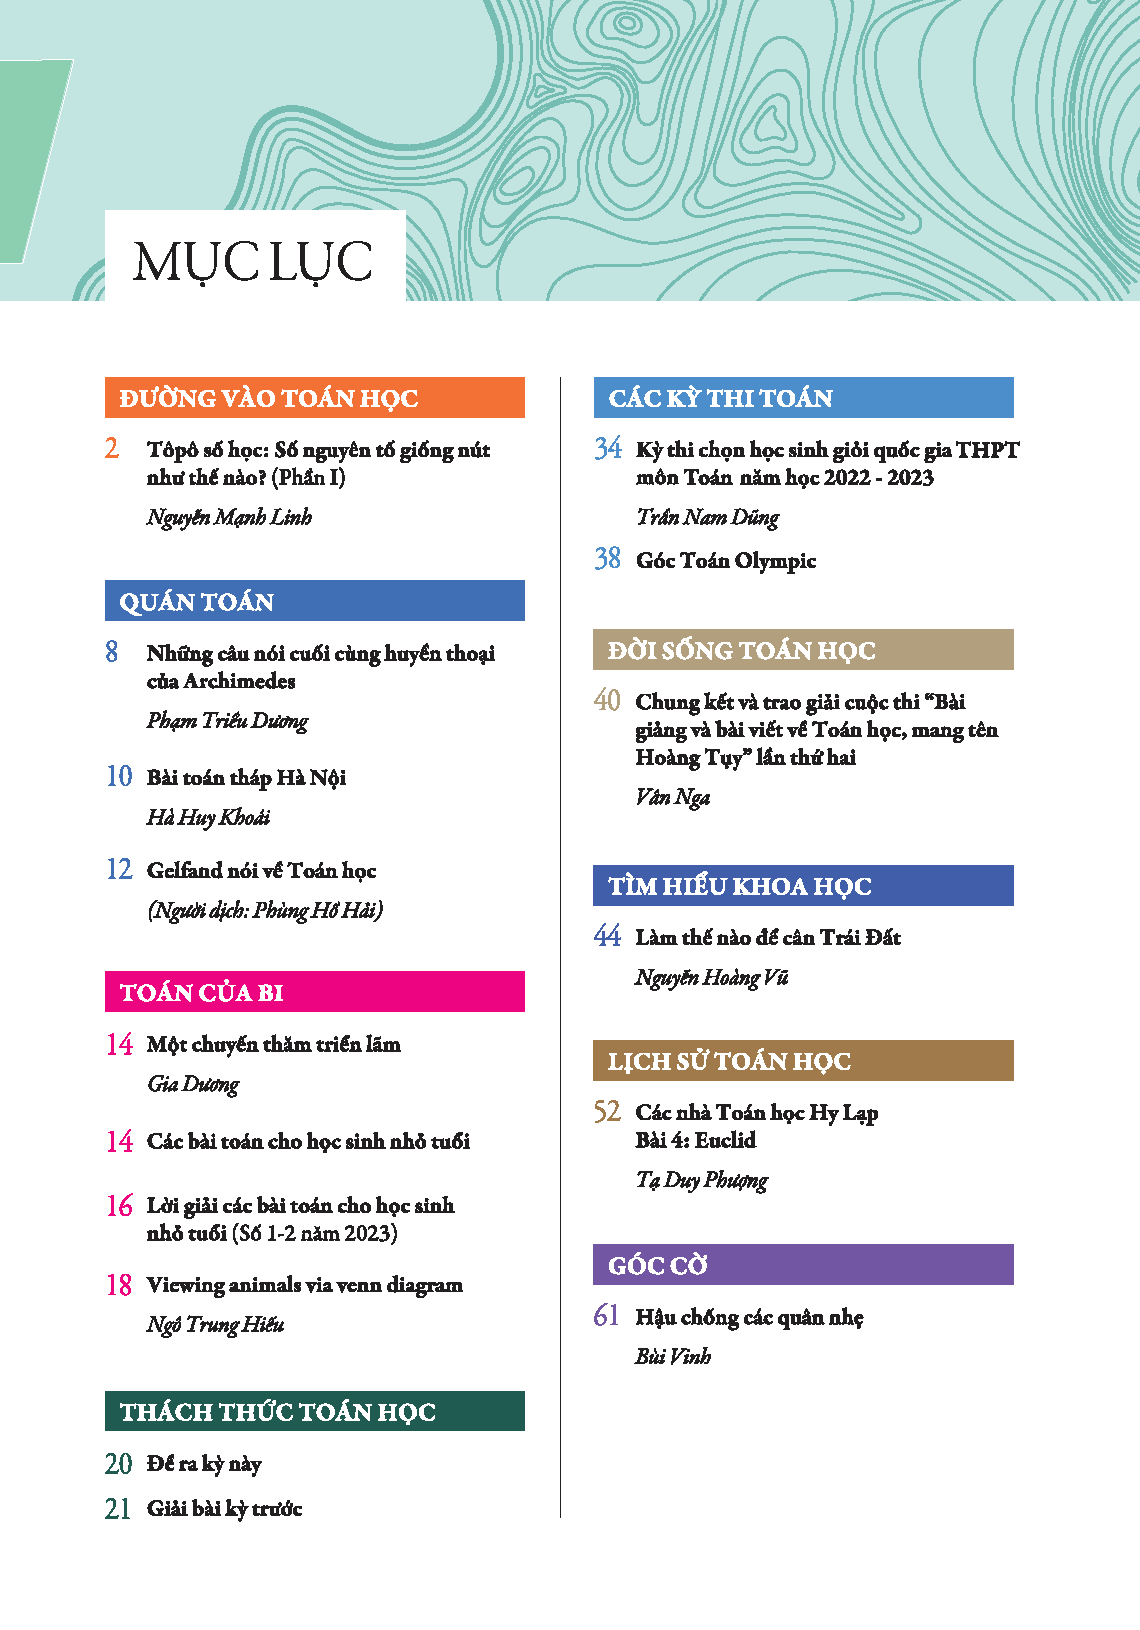
\includegraphics[scale=1]{ML.pdf}}}
%	 \centering
%	 \vspace*{0cm}
%	 \endgroup
%	 \newpage	  
%	 \pagestyle{empty}
%
%	\setcounter{page}{2}
%
%	\setcounter{figure}{0}
%	\thispagestyle{toanhocvadoisongnone}
\pagestyle{toanhocvadoisong}
\everymath{\color{toanhocdoisong}}
\graphicspath{{../toanhocdoisong/pic2/}}
\blfootnote{$^1$\color{toanhocdoisong}Accromath, vol. $11$, $2016$. (https://accromath.uqam.ca/2016/10/les-mosaiques-de-thiele/)}
\blfootnote{$^2$\color{toanhocdoisong}Đại học McGill, Canada. $^3$\color{toanhocdoisong}Đại học Copenhagen, Đan Mạch. $^4$Nghệ thuật Mới, hay Tân Nghệ thuật.}
\begingroup
\AddToShipoutPicture*{\put(0,616){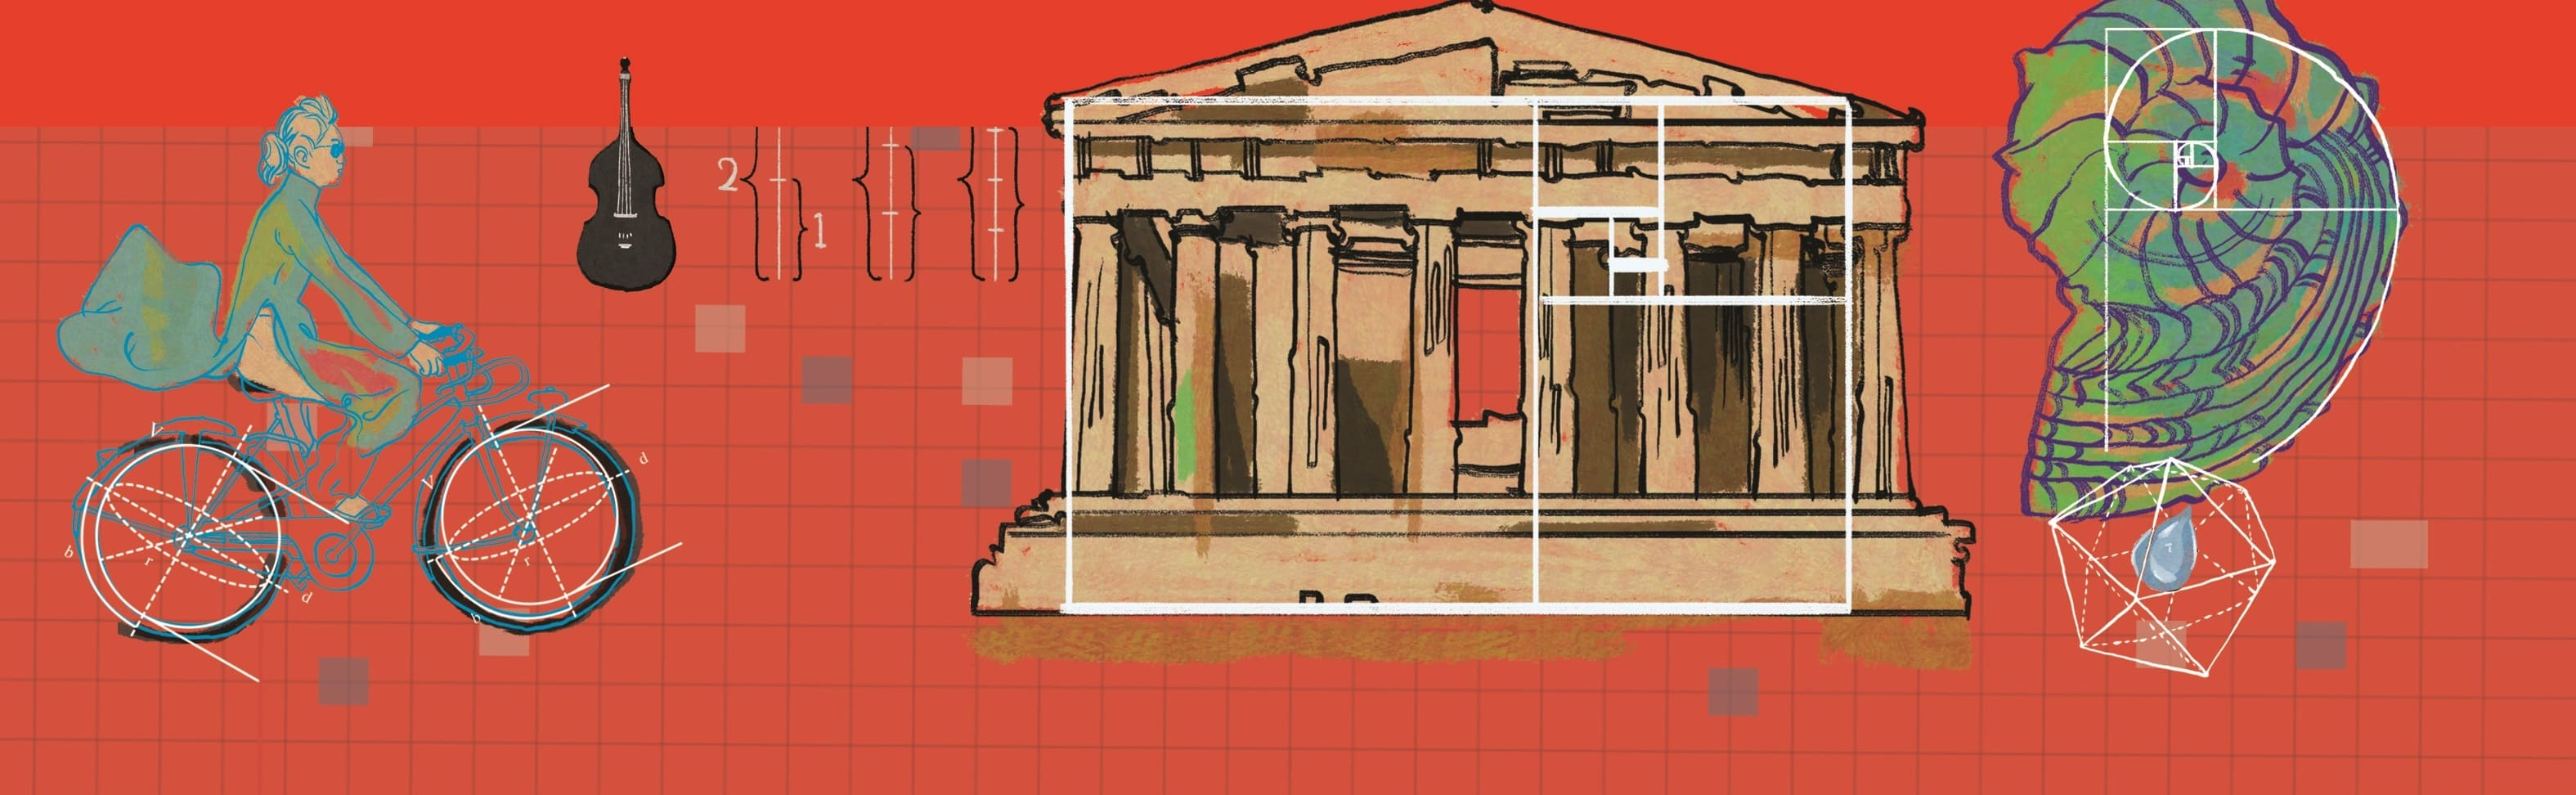
\includegraphics[width=19.3cm]{../bannertoanhocdoisong}}}
\AddToShipoutPicture*{\put(135,540){
\includegraphics[scale=1]{../tieude2.pdf}}}
\centering
\endgroup

\vspace*{165pt}
\begin{multicols}{2}
	\textit{Nhà thiên văn học, nhà thống kê và doanh nhân bảo hiểm người Đan Mạch Thorvald Thiele đã tìm ra cách sinh tự động các họa tiết khảm rất đẹp nhờ sử dụng khái niệm thặng dư bậc hai trong tập hợp các số nguyên\linebreak Gauss.}
	\vskip 0.1cm
	Tranh khảm gồm nhiều viên hoặc mảnh nhỏ nhiều màu sắc, làm từ những vật liệu khác nhau, được sắp xếp thành một họa tiết trang trí. Được dùng để lát sàn, trang trí tường, trần nhà và các đồ vật, tranh khảm rất được ưa chuộng ở thời Cổ Đại, và vẫn còn được sử dụng trong suốt thời Trung Cổ và Phục Hưng.
	\vskip 0.1cm
	Sau khi gần như biến mất, nghệ thuật lát khảm trở nên phổ biến trở lại với trào lưu nghệ thuật \textit{Art nouveau$^4$}  vào cuối thế kỷ $19$, đầu thế kỷ $20$. Những khám phá khoa học thu hút mạnh mẽ sự chú ý của công chúng và nhiều nghệ sỹ (gồm nhà thơ, nhạc sỹ, họa sỹ, v.v.) đã chuyển tải sức quyến rũ này bằng cách đưa thêm một chiều toán học vào tác phẩm của mình. Sự đều đặn duyên dáng của những họa tiết khảm tô điểm cho những ngôi nhà riêng cũng như những tòa nhà công cộng của chúng ta chỉ là một trong rất nhiều biểu hiện của cuộc tìm tòi thẩm mỹ này.
	\vskip 0.1cm
	Thorvald Thiele ($1838$ -- $1910$) đã đóng góp vào\, trào lưu\, này theo\, cách của\, riêng mình.
	\begin{figure}[H]
		\vspace*{-5pt}
		\centering
		\captionsetup{labelformat= empty, justification=centering}
		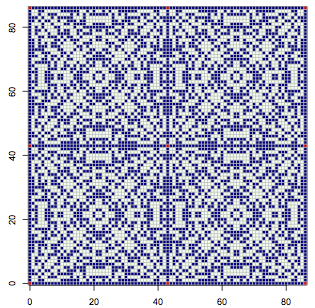
\includegraphics[width= 0.5\linewidth]{mosaique-1.png}
		\caption{\small\textit{\color{toanhocdoisong}Hình $1$. Thặng dư bậc hai modulo $43$.}}
		\vspace*{-10pt}
	\end{figure}
	Ông là người đầu tiên chỉ ra cách sử dụng thặng dư trong tập hợp các số nguyên Gauss để xây dựng một cách dễ dàng những hình khảm tuyệt đẹp. Trong Hình $2$ là hai họa tiết được ông công bố lần đầu tiên tại một hội nghị khoa học lớn của vùng Scandinavia tổ chức tại Copenhagen vào năm $1873$. Còn trong Hình $3$ là họa tiết Thiele ở sàn tiền sảnh Bộ Quốc phòng Đan Mạch, cũng ở Copenhagen.
	\begin{figure}[H]
		\vspace*{-5pt}
		\centering
		\captionsetup{labelformat= empty, justification=centering}
		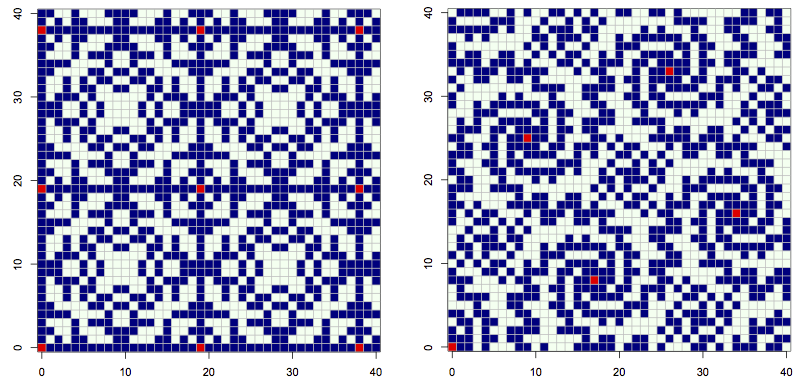
\includegraphics[width= 0.9\linewidth]{mosaique-2.png}
		\caption{\small\textit{\color{toanhocdoisong}Hình $2$. Hai họa tiết được Thiele công bố tại hội nghị khoa học năm $1873$.}}
		\vspace*{-5pt}
	\end{figure}
	Không chỉ tạo ra kết quả tuyệt đẹp, kỹ thuật xây dựng họa tiết khảm của Thiele vừa đơn giản lại vừa khéo léo. Nó dựa trên khái niệm thặng dư bậc hai phức mà chúng ta sẽ cùng nhau tìm hiểu dưới đây. Ở cuối bài, chúng ta sẽ đưa ra ba câu đố chưa có lời giải về họa tiết trong Hình $3$.
	\begin{figure}[H]
		\vspace*{-5pt}
		\centering
		\captionsetup{labelformat= empty, justification=centering}
		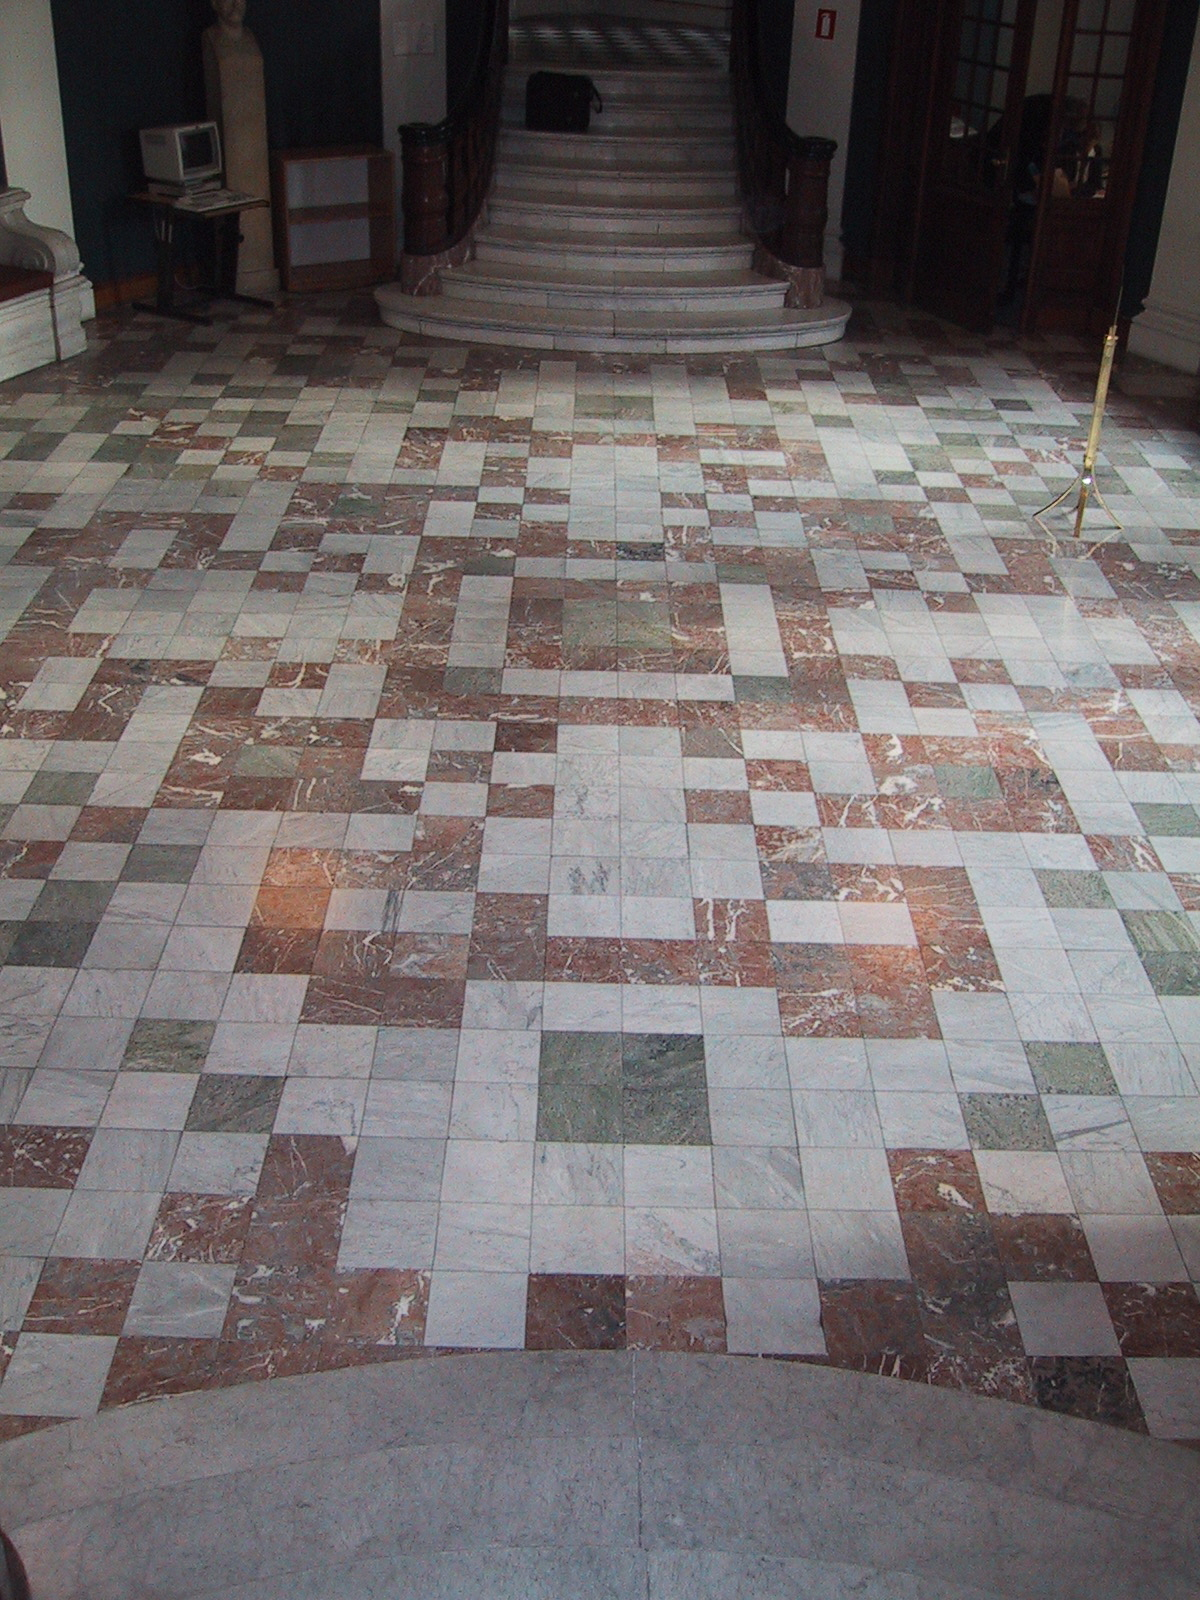
\includegraphics[width= 0.65\linewidth]{mosaique-3}
		\caption{\small\textit{\color{toanhocdoisong}Hình $3$. Họa tiết Thiele trang trí tiền sảnh Bộ Quốc Phòng Đan Mạch, số $9$ phố Holmens Kanal, Copenhagen.}}
		\vspace*{-10pt}
	\end{figure}
	\textbf{\color{toanhocdoisong}Đồng dư và thặng dư bậc hai trong $\pmb{\mathbb Z}$}
	\vskip 0.1cm
	Cho số nguyên $p \ge 1$. Nhắc lại rằng hai số nguyên
	\setlength{\abovedisplayskip}{5pt}
	\setlength{\belowdisplayskip}{5pt}
	\begin{align*}
		a, b \in \mathbb Z = \{ 0, \pm 1, \pm 2, \dots \}
	\end{align*}
	được gọi là đồng dư với nhau modulo $p$ nếu hiệu $a - b$ là bội của $p$, nghĩa là tồn tại $k \in \mathbb Z$ sao cho $a - b = kp$. Khi đó ta viết
	\begin{align*}
		a \equiv b \mod{p}.
	\end{align*}
	Nói riêng, $a$ đồng dư với số dư của nó khi chia cho $p$. Chẳng hạn, ta có thể viết $17 \equiv 1 \mod{4}$ vì $17 - 1 = 16$ chia hết cho $4$, hoặc $28 \equiv 0 \mod{4}$ vì $28 = 4 \times 7$ là bội của $4$.
	\vskip 0.1cm
	Ngoài ra, ta nói rằng số tự nhiên $q \in \mathbb N = \{ 0, 1, 2, \dots \}$ là một {\em thặng dư bậc hai} modulo $p$ nếu tồn tại số nguyên $x$ sao cho
	\begin{align*}
		q \equiv x^2 \mod{p}.
	\end{align*}
	Trong trường hợp ngược lại, ta nói $q$ không phải là thặng dư bậc hai modulo $p$.
	\vskip 0.1cm
	\textbf{\color{toanhocdoisong}Hai ví dụ đơn giản}
	\vskip 0.1cm
	\textbf{\color{toanhocdoisong}Ví dụ} $1.$ Mọi số tự nhiên $q$ đều là thặng dư bậc hai modulo $2$. Thật vậy:
	\vskip 0.1cm
	$\bullet$	Nếu $q \equiv 0 \mod{2}$, tức $q$ chẵn, thì $q \equiv 0^2 \mod{2}$;
	\vskip 0.1cm
	$\bullet$	Nếu $q \equiv 1 \mod{2}$, tức $q$ lẻ, thì $q \equiv 1^2 \mod{2}$.
	Một cách tổng quát, với mọi $p$, mọi số tự nhiên $q$ đồng dư với $0$ hoặc $1$ đều là thặng dư bậc hai modulo $p$.
	\vskip 0.1cm
	\textbf{\color{toanhocdoisong}Ví dụ} $2.$
	\vskip 0.1cm
	$\bullet$	Nếu $q \equiv 0 \mod{4}$, thì $q \equiv 0^2 \mod{4}$;
	\vskip 0.1cm
	$\bullet$	Nếu $q \equiv 1 \mod{4}$, thì $q \equiv 1^2 \mod{4}$.
	\vskip 0.1cm
	Trong khi đó, nếu $q \equiv 2 \mod{4}$ hoặc $q \equiv 3 \mod{4}$, không tồn tại số nguyên $x$ nào sao cho $q \equiv x^2 \mod{4}$. Điều này có thể được chứng minh bằng cách xét hai trường hợp $x$ chẵn và $x$ lẻ:
	\vskip 0.1cm
	$\bullet$	Nếu $x = 2n$ thì $x^2 = 4 n^2 \equiv 0 \mod{4}$;
	\vskip 0.2cm
	$\bullet$	Nếu $x = 2n + 1$ thì $x^2 = 4 n^2 + 4n + 1 \equiv 1 \mod{4}$.
	\vskip 0.2cm
	\textbf{\color{toanhocdoisong}Vỉa hè Thiele}
	\vskip 0.2cm
	Kết quả trên được minh họa trong Hình $4$ bằng ``vỉa hè Thiele". Một cách tổng quát, vỉa hè Thiele modulo $p$ gồm các mảnh hình vuông đơn vị đặt chính giữa các điểm $(0, 0)$, $(1, 0)$, $(2, 0)$, v.v. Màu của mảnh hình vuông tại điểm $(q, 0)$ được xác định như sau:
	\vskip 0.1cm
	$\bullet$	đỏ nếu $q \equiv 0 \mod{p}$;
	\vskip 0.1cm
	$\bullet$	xanh nếu $q$ là thặng dư bậc hai modulo $p$ (nhưng $q \not\equiv 0 \mod{p}$);
	\vskip 0.1cm
	$\bullet$	trắng nếu $q$ không phải thặng dư bậc hai modulo $p$.
	\begin{figure}[H]
		\vspace*{-5pt}
		\centering
		\captionsetup{labelformat= empty, justification=centering}
		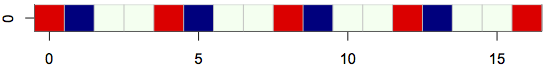
\includegraphics[width= 1\linewidth]{mosaique-4.png}
		\caption{\small\textit{\color{toanhocdoisong}Hình $4$. Vỉa hè Thiele modulo $4$.}}
		\vspace*{-10pt}
	\end{figure}
	Khi $p = 4$, mọi số tự nhiên $q$ đồng dư với $0$, $1$, $2$ hoặc $3$ modulo $4$. Họa tiết ``đỏ, xanh, trắng, trắng" ứng với các mảnh $(0, 0)$, $(1, 0)$, $(2, 0)$, $(3, 0)$ lặp lại vô hạn. Với mọi giá trị $p \ge 1$ khác, vỉa hè Thiele modulo $p$ có thể được xây dựng dễ dàng một khi ta đã biết màu của các mảnh $(0, 0), \dots, (p - 1, 0)$: họa tiết lặp lại với chu kỳ $p$.
	\vskip 0.2cm
	Các họa tiết khảm Thiele dựa trên một nguyên lý tương tự. Với mỗi cặp số nguyên $p = (p_1, p_2)$, màu của mảnh $(q_1, q_2)$ sẽ phụ thuộc vào việc $(q_1, q_2)$ có phải là thặng dư bậc hai modulo $p$ hay không. Để điều này có nghĩa, trước tiên chúng ta cần tìm hiểu khái niệm đồng dư giữa hai cặp số nguyên.
	\begin{tBox}
		\textbf{\textit{\color{toanhocdoisong}Thorvald Nicolai Thiele $\pmb{(1838 \!-\! 1910)}$}}
		\vskip 0.2cm
		\begin{wrapfigure}{l}{0.4\textwidth}
			\vspace*{-14pt}
			\centering
			\captionsetup{labelformat= empty, justification=centering}
			\hspace*{3pt}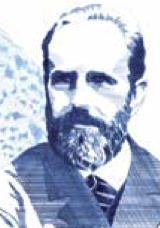
\includegraphics[width= 1.1\linewidth]{Thiele.png}
			\vspace*{-20pt}
		\end{wrapfigure}
		Thorvald Thiele sinh ngày $24$ tháng $12$ năm $1838$ ở Copenhagen và mất ngày $26$ tháng $9$ năm $1910$ ở cùng thành phố, thọ $71$ tuổi. Tên ông được đặt theo cha đỡ đầu của ông, nhà điêu khắc Bertel Thorvaldsen. Sau quá trình học tập xuất sắc, ông trở thành giáo sư thiên văn học tại Đại học Copenhagen từ năm $1875$ đến năm $1907$, đồng thời là giám đốc đài thiên văn của trường. Được coi là một người mở đường của thống kê toán học, ông là người đầu tiên đề xuất một lý thuyết chuyển động Brown, đồng thời là tác giả của các khái niệm cumulant và hàm hợp lý. Thiele cũng góp phần sáng lập Hafnia, công ty bảo hiểm nhân thọ tư nhân đầu tiên của của Đan Mạch, vào năm $1872$. Ông là giám đốc khoa học của công ty tới năm $1901$, rồi chủ tịch Hội đồng Quản trị từ năm $1903$ tới năm $1910$. Tên ông được đặt cho hai tiểu hành tinh; một trong  hai tiểu hành tinh đó được phát hiện bởi con trai ông, Holger Thiele, cũng là một nhà thiên văn học nổi tiếng.
	\end{tBox}
	\textbf{\color{toanhocdoisong}Mở rộng cho tập hợp các số nguyên Gauss}
	\vskip 0.1cm
	Trong công trình \textit{Disquisitiones arithmeticae\footnote[5]{\color{toanhocdoisong}Công ty phá sản năm $1993$.}}  xuất bản năm $1801$, nhà toán học, vật lý học và thiên văn học người Đức Carl Friedrich Gauss ($1777$ -- $1855$) quan tâm đến số học đồng dư trên những tập hợp khác $\mathbb Z$, trong đó có tập hợp các cặp số nguyên, tức là các vector $(a_1, a_2) \in \mathbb Z^2 = \mathbb Z \times \mathbb Z$.
	\vskip 0.1cm
	Gauss định nghĩa tổng và tích của hai phần tử bất kỳ $a = (a_1, a_2)$, $b = (b_1, b_2)$ trong $\mathbb Z^2$ như sau:
	\begin{align*}
		&(a_1, a_2) + (b_1, b_2) \\
		= \,&(a_1 + b_1, a_2 + b_2), \\
		&(a_1, a_2) \times (b_1, b_2) \\
		= \,&(a_1  b_1 - a_2  b_2, a_1  b_2 + a_2  b_1).
	\end{align*}
	Phép cộng là phép cộng vector thông thường. Phép nhân, có vẻ bí ẩn hơn, liên hệ mật thiết với khái niệm số phức (xem phần đóng khung bên dưới).
	\vskip 0.1cm
	Tập hợp $\mathbb Z^2$ được trang bị hai phép toán trên được gọi là tập hợp các {\em số nguyên Gauss}. Tập hợp các số nguyên Gauss có đủ các tính chất cần thiết để ta có thể định nghĩa trên đó các khái niệm đồng dư và thặng dư bậc hai tương tự những khái niệm đã có trên $\mathbb Z$.
	\vskip 0.1cm
	Cho hai số tự nhiên $p_1$ và $p_2$ không đồng thời bằng $0$. Ta nói rằng hai phần tử $a, b \in \mathbb Z$ đồng dư với nhau modulo $p = (p_1, p_2)$ nếu tồn tại $k = (k_1, k_2) \in \mathbb Z^2$ sao cho $a - b = k \times p$. Nói cách khác, $a \equiv b \mod{p}$ nếu và chỉ nếu
	\begin{align*}
		&(a_1, a_2) - (b_1, b_2) \\
		= \,&(k_1 p_1 - k_2 p_2, k_1 p_2 + k_2 p_1).
	\end{align*}
	Ta nói rằng $q = (q_1, q_2)$ là một {\em thặng dư bậc hai phức} modulo $p = (p_1, p_2)$ nếu tồn tại $x = (x_1, x_2) \in \mathbb Z^2$ sao cho $q \equiv x^2 \mod{p}$. Nói cách khác, ta cần tìm các số nguyên $x_1$ và $x_2$ sao cho
	\begin{align*}
		(q_1, q_2) \equiv (x_1^2 - x_2^2, 2 x_1 x_2) \mod{p}.
	\end{align*}
	\vskip 0.1cm
	\begin{tBox}
		\textbf{\textit{\color{toanhocdoisong}Mối liên hệ với số phức}}
		\vskip 0.1cm
		\begin{wrapfigure}{r}{0.4\linewidth}
			\vspace*{-15pt}
			\centering
			\captionsetup{labelformat= empty, justification=centering}
			\hspace*{-12pt}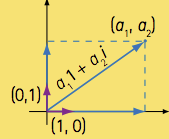
\includegraphics[width= 1.15\linewidth]{mosaique-6.png}
			\vspace*{-15pt}
		\end{wrapfigure}
		Các phép toán được Gauss định nghĩa trong $\mathbb Z^2$ có liên hệ mật thiết với khái niệm số phức. Một số phức là một số có dạng $a_1 + a_2 i$, ở đó $i = \sqrt{-1}$. Số phức có thể được biểu diễn trong mặt phẳng bằng cách đặt $1 = (1, 0)$ và $i = (0, 1)$, sao cho $(a_1, a_2) = a_1 1 + a_2 i$, mà ta có thể viết gọn là $a_1 + a_2 i$ mà không sợ nhầm lẫn. Thực hiện phép cộng và phép nhân thông thường với các biểu thức đại số $a_1 + a_2 i$ và $b_1 + b_2 i$, ta được:
		\begin{align*}
			&(a_1 + a_2 i) + (b_1 + b_2i) \\
			= \,&(a_1 + b_1) + (a_2 + b_2) i, \\
			&(a_1 + a_2i) \times (b_1 + b_2i) \\
			= \,&a_1 b_1 + (a_1 b_2 + a_2 b_1) i + a_2 b_2 i^2 \\
			= \,&( a_1  b_1 - a_2  b_2) + (a_1 b_2 + a_2 b_1) i ,
		\end{align*}
		ở đó ta đã thay $i^2 = -1$.
		\vskip 0.1cm
		Để ý rằng phép nhân với $i$ tương đương với phép quay một góc $\pi / 2$ ngược chiều kim đồng hồ. Thật vậy:
		\begin{align*}
			(a_1 + a_2 i) \times i = a_1 i + a_2 i^2 = -a_2 + a_1 i.
		\end{align*}
		\begin{wrapfigure}{r}{0.4\linewidth}
			\vspace*{-15pt}
			\centering
			\captionsetup{labelformat= empty, justification=centering}
			\hspace*{-12pt}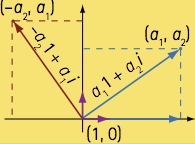
\includegraphics[width= 1.1\linewidth]{mosaique-7.png}
			\vspace*{-15pt}
		\end{wrapfigure}
		Khi $a_2 = 0$, số là {\em số thực}, còn khi $a_1 = 0$, số là {\em số ảo}.
		Các phép toán được định nghĩa trong tập hợp các số phức chính là các phép toán trong tập hợp các số nguyên Gauss. Tập hợp $\mathbb Z^2$ cùng với hai phép toán này thường được ký hiệu là $\mathbb Z[i]$.
	\end{tBox}
	\vskip 0.1cm
	\textbf{\color{toanhocdoisong}Hình khảm Thiele}
	\vskip 0.1cm
	Cũng như vỉa hè Thiele, một hình khảm Thiele modulo $p = (p_1, p_2)$ gồm nhiều mảnh hình vuông đơn vị phủ kín mặt phẳng. Màu của mảnh tại điểm $q = (q_1, q_2)$ được xác định như sau:
	\vskip 0.1cm
	$\bullet$	đỏ nếu $q \equiv 0 \mod{p}$;
	\vskip 0.1cm
	$\bullet$	xanh nếu $q$ là thặng dư bậc hai phức modulo $p$ (nhưng $q \not\equiv 0 \mod{p}$);
	\vskip 0.1cm
	$\bullet$	trắng nếu $q$ không phải thặng dư bậc hai phức modulo $p$.
	\vskip 0.1cm
	Ví dụ, giả sử $p = (2, 0)$. Ta có:
	\begin{align*}
		&(a_1, a_2) \equiv (b_1, b_2) \mod{p} \\
		\iff& a_1 - b_1 = 2 k_1 \mbox{ và } a_2 - b_2 = 2 k_2,
	\end{align*}
	tức là $a_1 \equiv b_1 \mod{2}$ và $a_2 \equiv b_2 \mod{2}$. Suy ra với mọi $(a_1, a_2) \in \mathbb Z^2$, $(a_1, a_2) \equiv (0, 0), (0, 1), (1, 0)$ hoặc $(1, 1) \mod{p = (2, 0)}$.
	\vskip 0.1cm
	Từ nhận xét trên, để xây dựng hình khảm Thiele tương ứng, ta chỉ cần xét xem $(0, 0), (0, 1), (1, 0)$ và $(1, 1)$ có phải thặng dư bậc hai phức modulo $p = (2, 0)$ hay không.
	\vskip 0.1cm
	Như vậy, với $a_1, a_2 \in \{0, 1\}$, ta cần kiểm tra xem có tồn tại hay không $x_1, x_2 \in \mathbb Z$ sao cho
	\begin{align*}
		a_1 \equiv x_1^2 - x_2^2 \mod{2}, a_2 \equiv 2 x_1 x_2 \mod{2}.
	\end{align*}
	Nếu $a_2 = 0$, chỉ cần chọn $x_1 = a_1$ và $x_2 = 0$. Nhưng nếu $a_2 = 1$ thì không thể tìm được $x_1, x_2 \in \mathbb Z$ thỏa mãn vì $2 x_1 x_2$ luôn chẵn.
	\vskip 0.1cm
	Kết quả này được mình họa trong Hình $5$. Các mảnh $(0, 0)$, $(1, 0)$, $(0, 1)$ và $(1, 1)$ tạo thành họa tiết cơ bản (bên trái) mà chúng ta có thể lặp lại một số lần tùy ý (bên phải). Hiệu ứng ảo giác của hình vẽ được tạo bởi sự tuần hoàn kép (cả chiều ngang lẫn chiều dọc) của họa tiết cùng với các màu sắc tương phản mạnh.
	\begin{figure}[H]
		\vspace*{-5pt}
		\centering
		\captionsetup{labelformat= empty, justification=centering}
		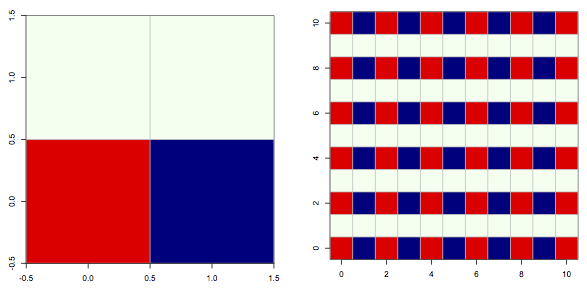
\includegraphics[width= 1\linewidth]{mosaique-8.png}
		\caption{\small\textit{\color{toanhocdoisong}Hình $5$. Hình khảm Thiele modulo $p = (2, 0)$.}}
		\vspace*{-10pt}
	\end{figure}
	Hai thí dụ khác, do chính Thiele đưa ra, được trình bày trong Hình $2$ (hình này được vẽ bằng một phần mềm miễn phí, với hướng dẫn tải và sử dụng ở cuối bài). Hình khảm bên trái tương ứng với $p = (19, 0)$; có thể dễ dàng nhận thấy nó tuần hoàn theo chiều dọc và chiều ngang. Hình khảm bên phải tương ứng với $p = (17, 8)$; chúng ta cũng nhận có sự đều đặn, nhưng việc xác định chính xác nó thì không hiển nhiên như trường hợp trước.
	\vskip 0.1cm
	\textbf{\color{toanhocdoisong}Ý nghĩa hình học}
	\vskip 0.1cm
	Để hiểu rõ hơn quy luật của hình khảm Thiele, chúng ta hãy coi các phần tử của $\mathbb Z^2$ như các vector tọa độ nguyên. Để ý rằng theo định nghĩa, hai vector $a = (a_1, a_2)$ và $b = (b_1, b_2)$ đồng dư với nhau modulo $p = (p_1, p_2)$ nếu và chỉ nếu
	\begin{align*}
		&(a_1, a_2) - (b_1, b_2) \\
		= \,&(k_1 p_1 - k_2 p_2, k_1 p_2 + k_2 p_1) \\
		= \,&k_1 (p_1, p_2) + k_2 (-p_2, p_1) ,
	\end{align*}
	nghĩa là nếu hiệu của chúng có thể viết thành tổng của một bội của $p$ và một bội của vector $p' = (-p_2, p_1)$ vuông góc với $p$.
	\vskip 0.1cm
	Trong ngôn ngữ hình học, điều này có nghĩa là hai vector $a$ và $b$ đồng dư với nhau modulo $p$ nếu có thể đi từ $a$ tới $b$ (hoặc ngược lại) bằng một số hữu hạn các tịnh tiến theo $p$, $-p$, $p'$ và $-p'$. Đặc biệt, tất cả các vector [trong $\mathbb Z^2$] đều đồng dư với một vector nằm trong hình vuông có bốn đỉnh $(0, 0)$, $p$, $p'$ và $p + p'$. Tính chất này là tương đương trong $\mathbb Z^2$ của phép chia có dư trong $\mathbb Z$.
	\vskip 0.1cm
	Quay trở lại với hình bên phải của Hình $2$, chúng ta có thể kiểm tra rằng họa tiết cơ bản quả đúng là phần được giới hạn bởi bốn điểm đỏ $(9, 25)$, $(17, 8)$, $(26, 33)$ và $(34, 16)$.
	\vskip 0.1cm
	\PIbox{\textbf{\color{toanhocdoisong}\textit{Có bao nhiêu mảnh được tô màu?}}
		\vskip 0.1cm
		Kinh nghiệm cho thấy những hình khảm Thiele đẹp nhất khi $p = (p_1, p_2)$ là một {\em số nguyên tố Gauss}, nghĩa là nếu với mọi $a, b \in \mathbb Z^2$:
		\begin{align*}
			&a \times b \equiv (0, 0) \mod{p} \\
			\implies &a \equiv (0, 0) \mbox{ hoặc } b \equiv (0, 0) \mod{p}.
	\end{align*}}
	\PIbox{
		Có thể chứng minh được rằng $p$ là số nguyên tố Gauss nếu và chỉ nếu một trong ba điều kiện sau được thỏa mãn (chúng ta thừa nhận kết quả này):
		\vskip 0.1cm
		$\bullet$	Nếu $p_1 \ge 1$ và $p_2 \ge 1$: $p_1^2 + p_2^2$ là số nguyên tố theo nghĩa thông thường;
		\vskip 0.1cm
		$\bullet$	Nếu $p_1 = 0$ và $p_2 \ge 1$: $|p_2|$ nguyên tố và $|p_2| \equiv 3 \mod{4}$;
		\vskip 0.1cm
		$\bullet$	Nếu $p_1 \ge 1$ và $p_2 = 0$: $|p_1|$ nguyên tố và $|p_1| \equiv 3 \mod{4}$.
		\vskip 0.1cm
		Như vậy, $(19, 0)$, $(71, 0)$ và $(17, 8)$ là các số nguyên tố Gauss, nhưng $(5, 0)$ thì không phải, và ta có $(5, 0) = (1, 2) \times (1, -2)$.
		\vskip 0.1cm
		Ta biết rằng nếu $p$ là một số nguyên tố, một nửa các số từ $1$ đến $p - 1$ là thặng dư bậc hai modulo $p$. Nói cách khác, có $(p - 1) / 2$ mảnh màu xanh trong họa tiết cơ bản của vỉa hè Thiele modulo $p$. Tương tự, bằng cách sử dụng các khái niệm trong lý thuyết trường, có thể chứng minh rằng nếu $p = (p_1, p_2)$ là số nguyên tố Gauss với $p_1 \ge 1$ và $p_2 \ge 1$, thì có $p_1^2 + p_2^2 - 1$ mảnh màu xanh trong họa tiết cơ bản của hình khảm Thiele modulo $p$.}
	\vskip 0.2cm
	\textbf{\color{toanhocdoisong}Trở lại bức hình tiền sảnh}
	\vskip 0.1cm
	Sàn sảnh trong Hình $3$ được lát theo hình khảm Thiele modulo $(71, 0)$. Họa tiết cơ bản của nó được cho trong Hình $6$. Ngày nay thuộc Bộ Quốc phòng Đan Mạch, tòa nhà có sàn lát này từng là trụ sở của công ty bảo hiểm Hafnia. Ở cương vị chủ tịch Hội đồng Quản trị của công ty, Thiele đã cho phép khởi công xây tòa nhà vào tháng $5$ năm $1910$, chỉ vài tháng trước khi ông qua đời ở tuổi $71$. Người ta cho rằng họa tiết lát sảnh được chọn sau khi Thiele mất, để tưởng nhớ ông.
	\vskip 0.1cm
	Chúng ta có thể rút ra ba quan sát về hình lát sàn này như sau:
	\vskip 0.1cm
	$\bullet$ Có một số lỗi trong việc thể hiện họa tiết. Thực vậy, mặc dù $(27, 35)$ là thặng dư bậc hai modulo $p = (71, 0)$, viên gạch lát tương ứng lại có màu trắng. Đây có thể là một lỗi tính toán, vì nó xuất hiện đến bảy lần trên toàn bộ tác phẩm.
	\begin{figure}[H]
		\vspace*{-5pt}
		\centering
		\captionsetup{labelformat= empty, justification=centering}
		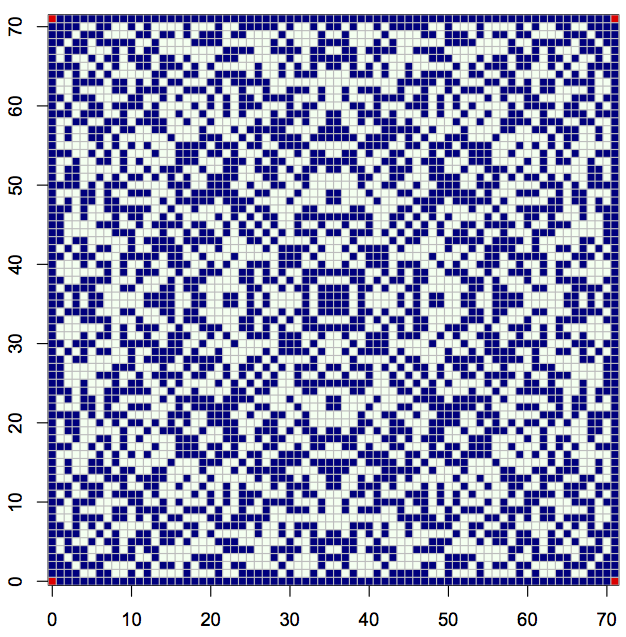
\includegraphics[width= 0.85\linewidth]{mosaique-9.png}
		\caption{\small\textit{\color{toanhocdoisong}Hình $6$. Hình khảm Thiele modulo $(71, 0)$, được dùng làm mẫu lát sàn tiền sảnh Bộ Quốc phòng Đan Mạch.}}
		\vspace*{-10pt}
	\end{figure}
	$\bullet$ Khi so sánh Hình $3$ và Hình $6$, chúng ta thấy mảnh $(25, 45)$ đúng ra phải màu trắng, nhưng trên sàn gạch thực tế lại màu đỏ. Lỗi này không lặp lại ở những chỗ khác. Không rõ đây là do sự lơ đãng của người thợ lát, hay do truyền thống nghề nghiệp không muốn sự hoàn hảo?
	\begin{figure}[H]
		\vspace*{-5pt}
		\centering
		\captionsetup{labelformat= empty, justification=centering}
		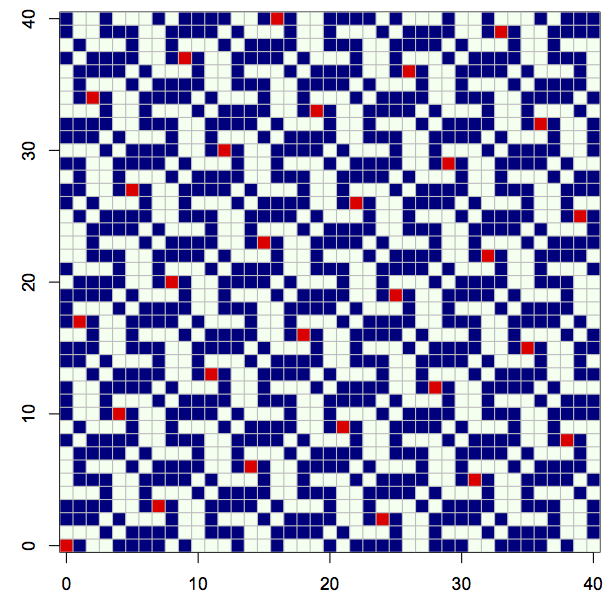
\includegraphics[width= 0.85\linewidth]{mosaique-10.png}
		\caption{\small\textit{\color{toanhocdoisong}Hình $7$. Thặng dư bậc hai modulo $(7, 3)$. Hình khảm này được tạo với một số không nguyên tố: $(7, 3) = (1, -1) \times (2, 5)$.}}
		\vspace*{-10pt}
	\end{figure}
	$\bullet$ Vì sao một số viên gạch tương ứng với thặng dư bậc hai có màu đỏ, trong khi những viên khác lại xanh lá cây? Liệu có phải chỉ đơn giản vì lý do thẩm mỹ? Tính cân đối của họa tiết gợi ý rằng hai màu này thể hiện một tính chất khác của các thặng dư bậc hai. Nhưng đó là tính chất gì?
	\vskip 0.1cm
	Có thể lục lại các tài liệu lưu trữ của công ty Hafnia để tìm câu trả lời cho hai câu hỏi đầu tiên. Câu hỏi thứ ba thì có bản chất thuần túy toán học và việc giải đáp nó có thể cần đến các tính chất của các số nguyên Gauss, của thặng dư bậc hai (hay bậc bốn?) phức và các chủ đề hấp dẫn khác của lý thuyết số. Câu trả lời vẫn là bí ẩn, và việc tìm ra nó được dành cho các bạn!
	\vskip 0.2cm
	\PIbox{
	\textbf{\color{toanhocdoisong}\textit{Vẽ tranh khảm Thiele bằng R}}
	\vskip 0.1cm
	Chúng ta có thể dễ dàng tạo ra một hình khảm Thiele nhờ một chương trình được viết bởi S{\o}ren Buhl, giáo sư toán và thống kê, Đại học Aalborg (Đan Mạch). Chương trình của ông được viết bằng ngôn ngữ R, có thể được tải miễn phí cho Windows, MacOS hoặc Linux tại:
	\url{http://www.r-project.org/}
	\vskip 0.1cm
	Chương trình vẽ có thể được tải ở đây:
	\url{http://www.math.mcgill.ca/cgenest/Thiele.R}
	\vskip 0.1cm
	Sau khi sao chép đoạn mã của chương trình vào cửa sổ lệnh của R, ta có thể vẽ một hình khảm Thiele modulo $p$ với kích thước $(n + 1) \times (n + 1)$ bằng lệnh $tuile(p, n)$. Thí dụ, Hình $2$ là kết quả của các lệnh $tuile(19,40)$ và $tuile(17 + 8i, 40)$. Hình $5$ nhận được bằng cách nhập lệnh $tuile(71, 71)$.}
	\vskip 0.1cm
	\textbf{\color{toanhocdoisong}Tài liệu tham khảo}
	\vskip 0.1cm
	[$1$] Décaillot, A.--M. ($2002$). Géométrie des tissus, mosaïques, échiquiers: Mathématiques curieuses et utiles. \textit{Revue d'histoire des mathématiques}, vol. $8$, pp. $145-206$.
	\vskip 0.1cm
	[$2$] Lauritzen, S., \textit{Thiele: Pioneer in Statistics}, Oxford University Press, $2002$.
\end{multicols}
%	\newpage
%	
	\setcounter{figure}{0}
	\thispagestyle{duongvaotoanhocnone}
\pagestyle{duongvaotoanhoc}
\everymath{\color{duongvaotoanhoc}}
\graphicspath{{../duongvaotoanhoc/pic/}}
\blfootnote{$^1$\color{duongvaotoanhoc}Universit\'e Paris--Saclay.}
\begingroup
\AddToShipoutPicture*{\put(0,616){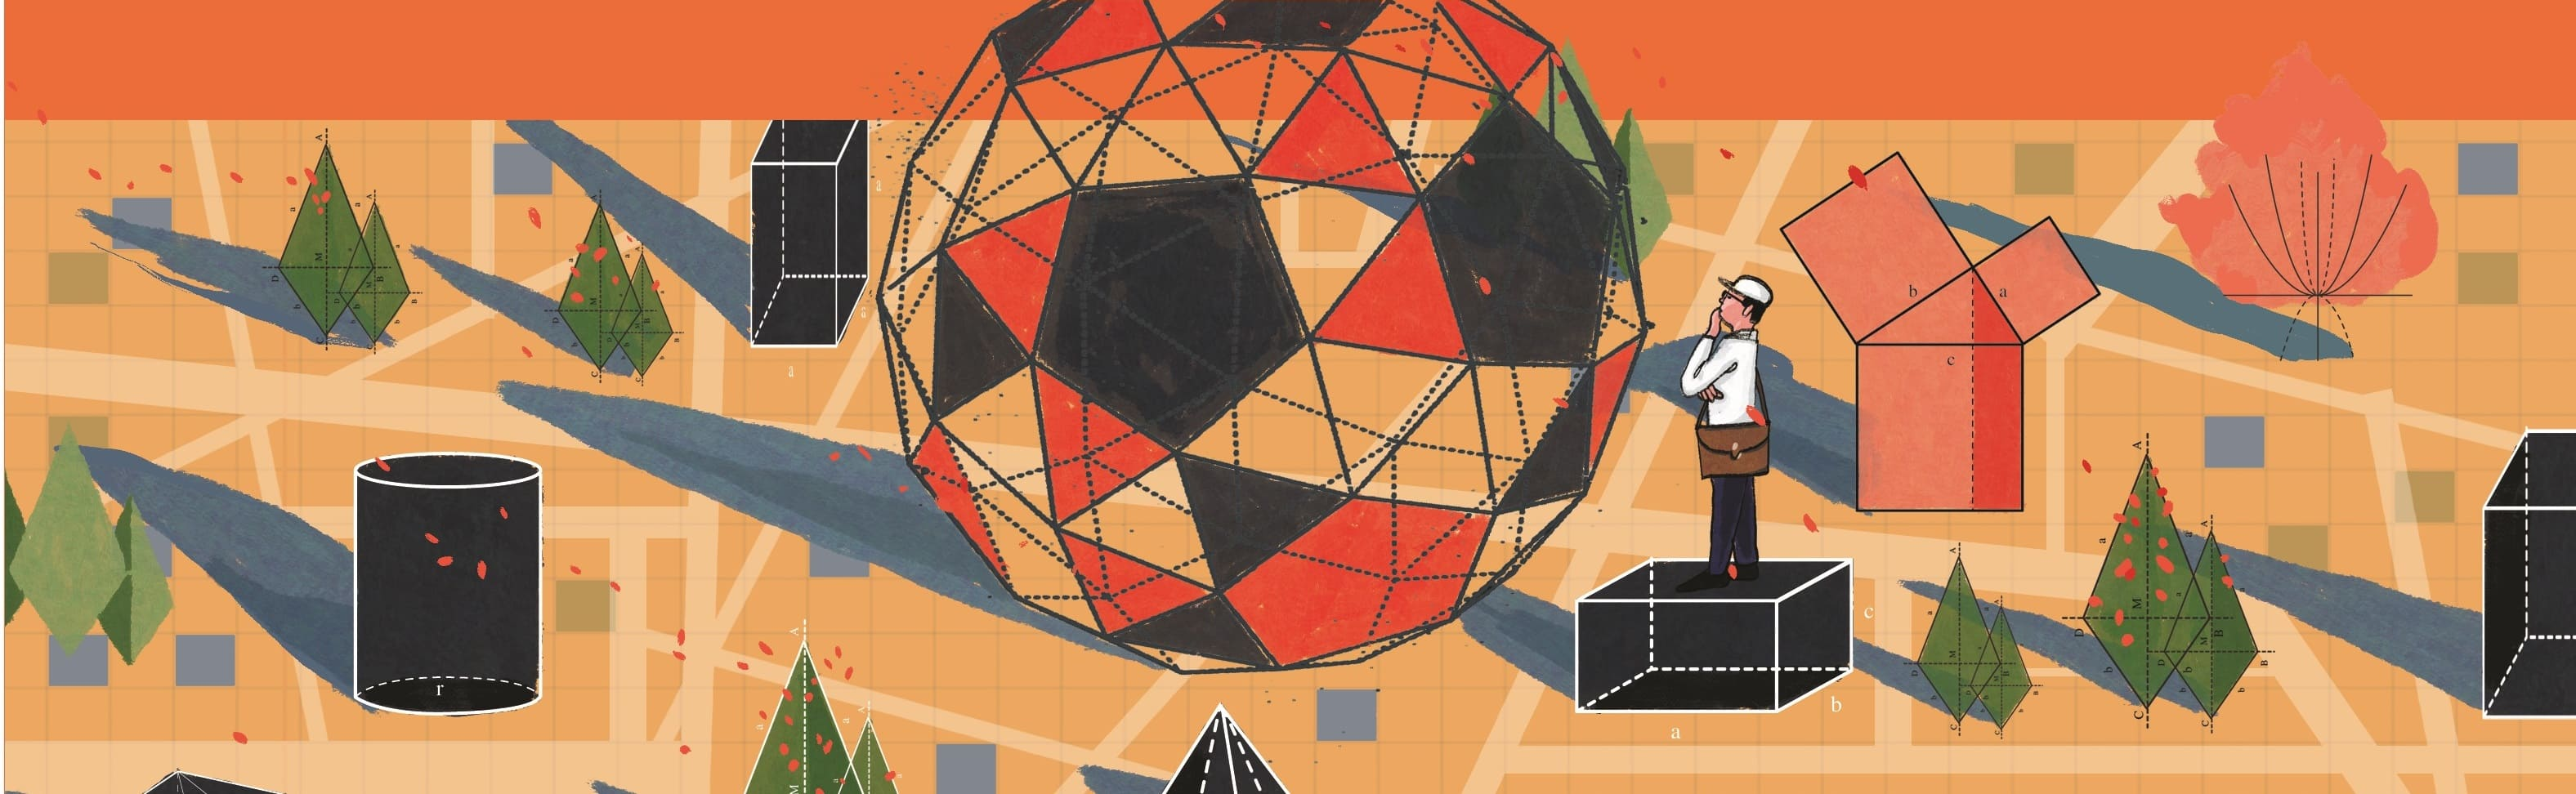
\includegraphics[width=19.3cm]{../bannerduongvao}}}
\AddToShipoutPicture*{\put(90,522){
\includegraphics[scale=1]{../tieude.pdf}}}
\centering
\endgroup
\vspace*{185pt}

\begin{multicols}{2}	
	Tôpô học là lĩnh vực nghiên cứu các không gian trừu tượng, những đối tượng liên tục. Ngược lại, số học là lĩnh vực nghiên cứu các số nguyên, những đối tượng rời rạc. Hai lĩnh vực này dường như nằm ở hai thái cực đối lập của toán học. Đấy là cho đến khoảng vài thập kỷ trở lại đây, khi các nhà toàn học phát hiện ra mối liên hệ giữa hai đối tượng tưởng như chẳng liên quan ở hai bên. Người ta đang xây dựng một cầu nối, một cuốn từ điển cho phép dịch các định lý từ một bên sang bên kia và ngược lại. Lĩnh vực mới toanh này được gọi là {\bf\color{duongvaotoanhoc} tôpô số học}.
	\vskip 0.1cm
	\textbf{\color{duongvaotoanhoc}Nhóm cơ bản}
	\vskip 0.1cm
	Để nói về tôpô số học, tất nhiên ta phải bắt đầu với... tôpô học và số học. Các không gian tôpô là các đối tượng cho phép ta nói về lân cận của các điểm, cũng như các hàm liên tục. Sự ``giống nhau'' giữa các không gian tôpô được cho bởi các {phép đồng phôi}, các hàm liên tục $1-1$ mà hàm ngược cũng liên tục. Để đơn giản, ta sẽ chỉ quan tâm đến các không gian {\bf\color{duongvaotoanhoc} liên thông}: hai điểm bất kỳ luôn nối được bằng một đường. Một {\bf\color{duongvaotoanhoc} đường} giữa hai điểm $x$, $y$ trong một không gian tôpô $X$ đơn giản là một hàm liên tục $f: I \to X$ sao cho $f(0) = x$ và $f(1) = y$.
	\vskip 0.1cm
	Giả sử ta có một đường khác $g: I \to X$ từ $x$ đến $y$. Không gì cản chúng ta nói về khái niệm ``đường giữa hai đường $f$ và $g$'', mà toán học gọi là {\bf\color{duongvaotoanhoc} đồng luân}. Đó là một hàm liên tục $H: I \times I \to X$ sao cho $H(t,0) = f(t)$, $H(t,1) = g(t)$, $H(0,s) = x$ và $H(1,s) = y$. Nói cách khác, $H$ là một họ các đường trung gian được tham số hóa bởi $s$, thể hiện sự biến dạng liên tục từ đường $f$ (khi $s=0$) đến đường $g$ (khi $s = 1$), đồng thời giữ cố dịnh hai đầu mút $x$, $y$. 
	\begin{figure}[H]
		\vspace*{-5pt}
		\centering
		\captionsetup{labelformat= empty, justification=centering}
		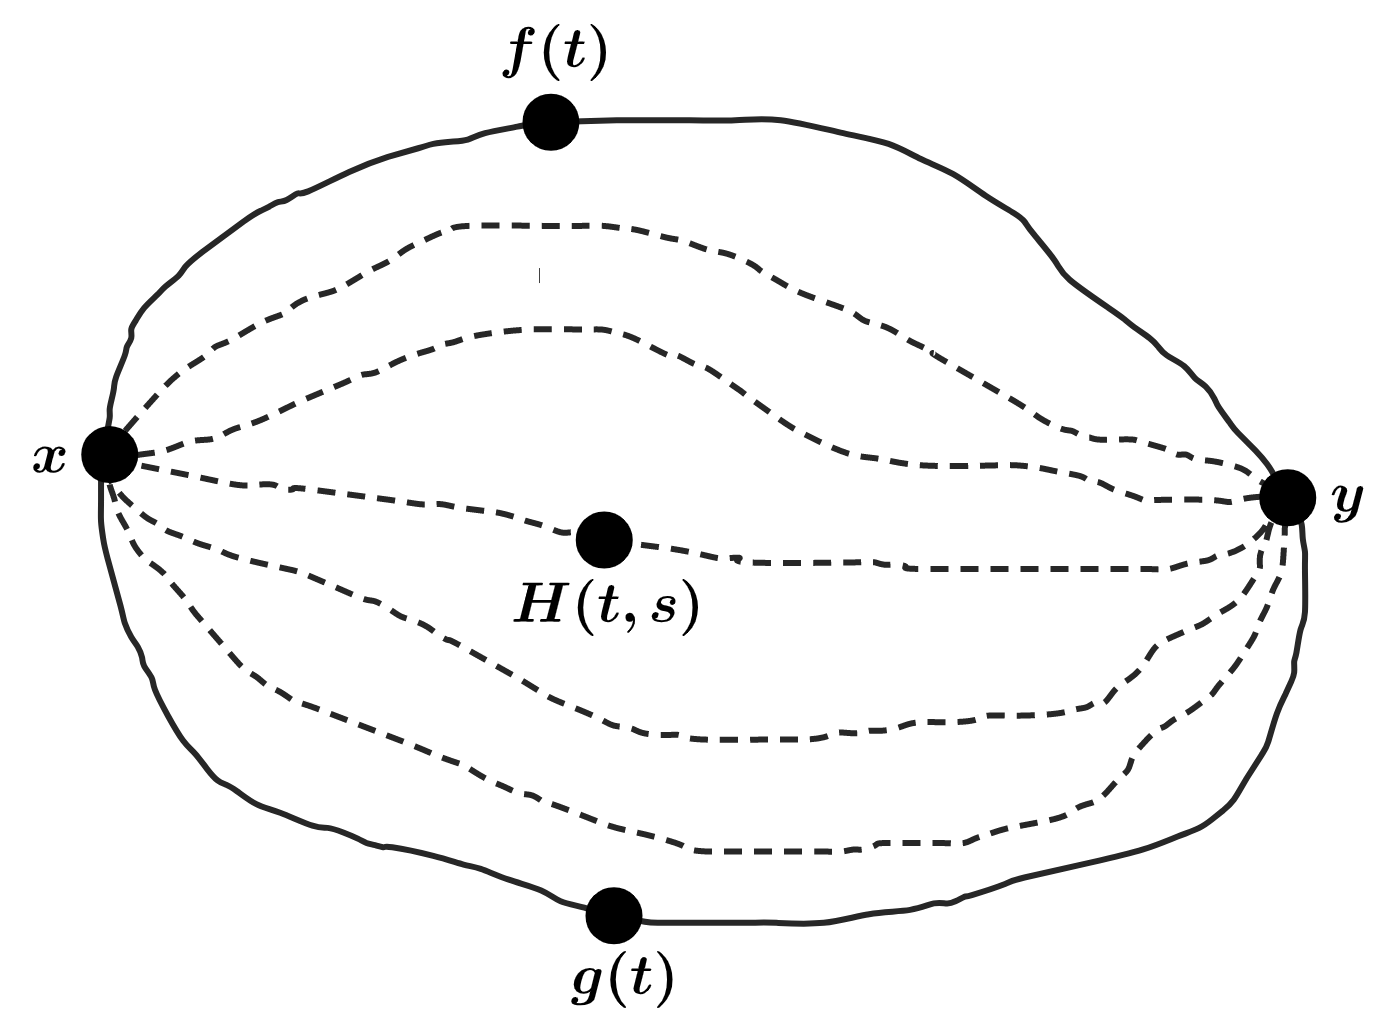
\includegraphics[width= 0.9\linewidth]{h1.png}
		\caption{\small\textit{\color{duongvaotoanhoc}Hình $1$: Một phép đồng luân giữa hai đường $f$ và $g$.}}
		\vspace*{-10pt}
	\end{figure}
	Khi $H$ tồn tại, ta nói hai đường $f$ và $g$ đồng luân, ký hiệu bởi $f \sim g$. Khi hai đường bất kỳ giữa hai điểm cho trước luôn đồng luân, ta nói không gian $X$ {\bf\color{duongvaotoanhoc} đơn liên}. Ví dụ về không gian đơn liên là không gian Euclid $\mathbb{R}^n$. Thật vậy, cấu trúc cộng và nhân với vô hướng trong $\mathbb{R}^n$ cho phép ta định nghĩa phép đồng luân $H(t,s) = (1-s) \cdot f(t) + s \cdot g(t)$ giữa hai đường $f, g$ tùy ý. Mặt  siêu cầu $\mathbb{S}^n$, thu được bằng cách thêm một điểm ở xa vô tận vào $\mathbb{R}^n$, cũng đơn liên với $n > 1$: hãy chọn một điểm P tùy ý trên mặt cầu và hình dung rằng mọi đường đều có thể biến dạng liên tục thành một đường không đi qua $P$. Mà $\mathbb{R}^n$ bỏ đi $P$ chính là (đồng phôi với) $\mathbb{R}^n$, nên hai đường không đi qua $P$ luôn đồng luân.
		\begin{figure}[H]
		\vspace*{-5pt}
		\centering
		\captionsetup{labelformat= empty, justification=centering}
		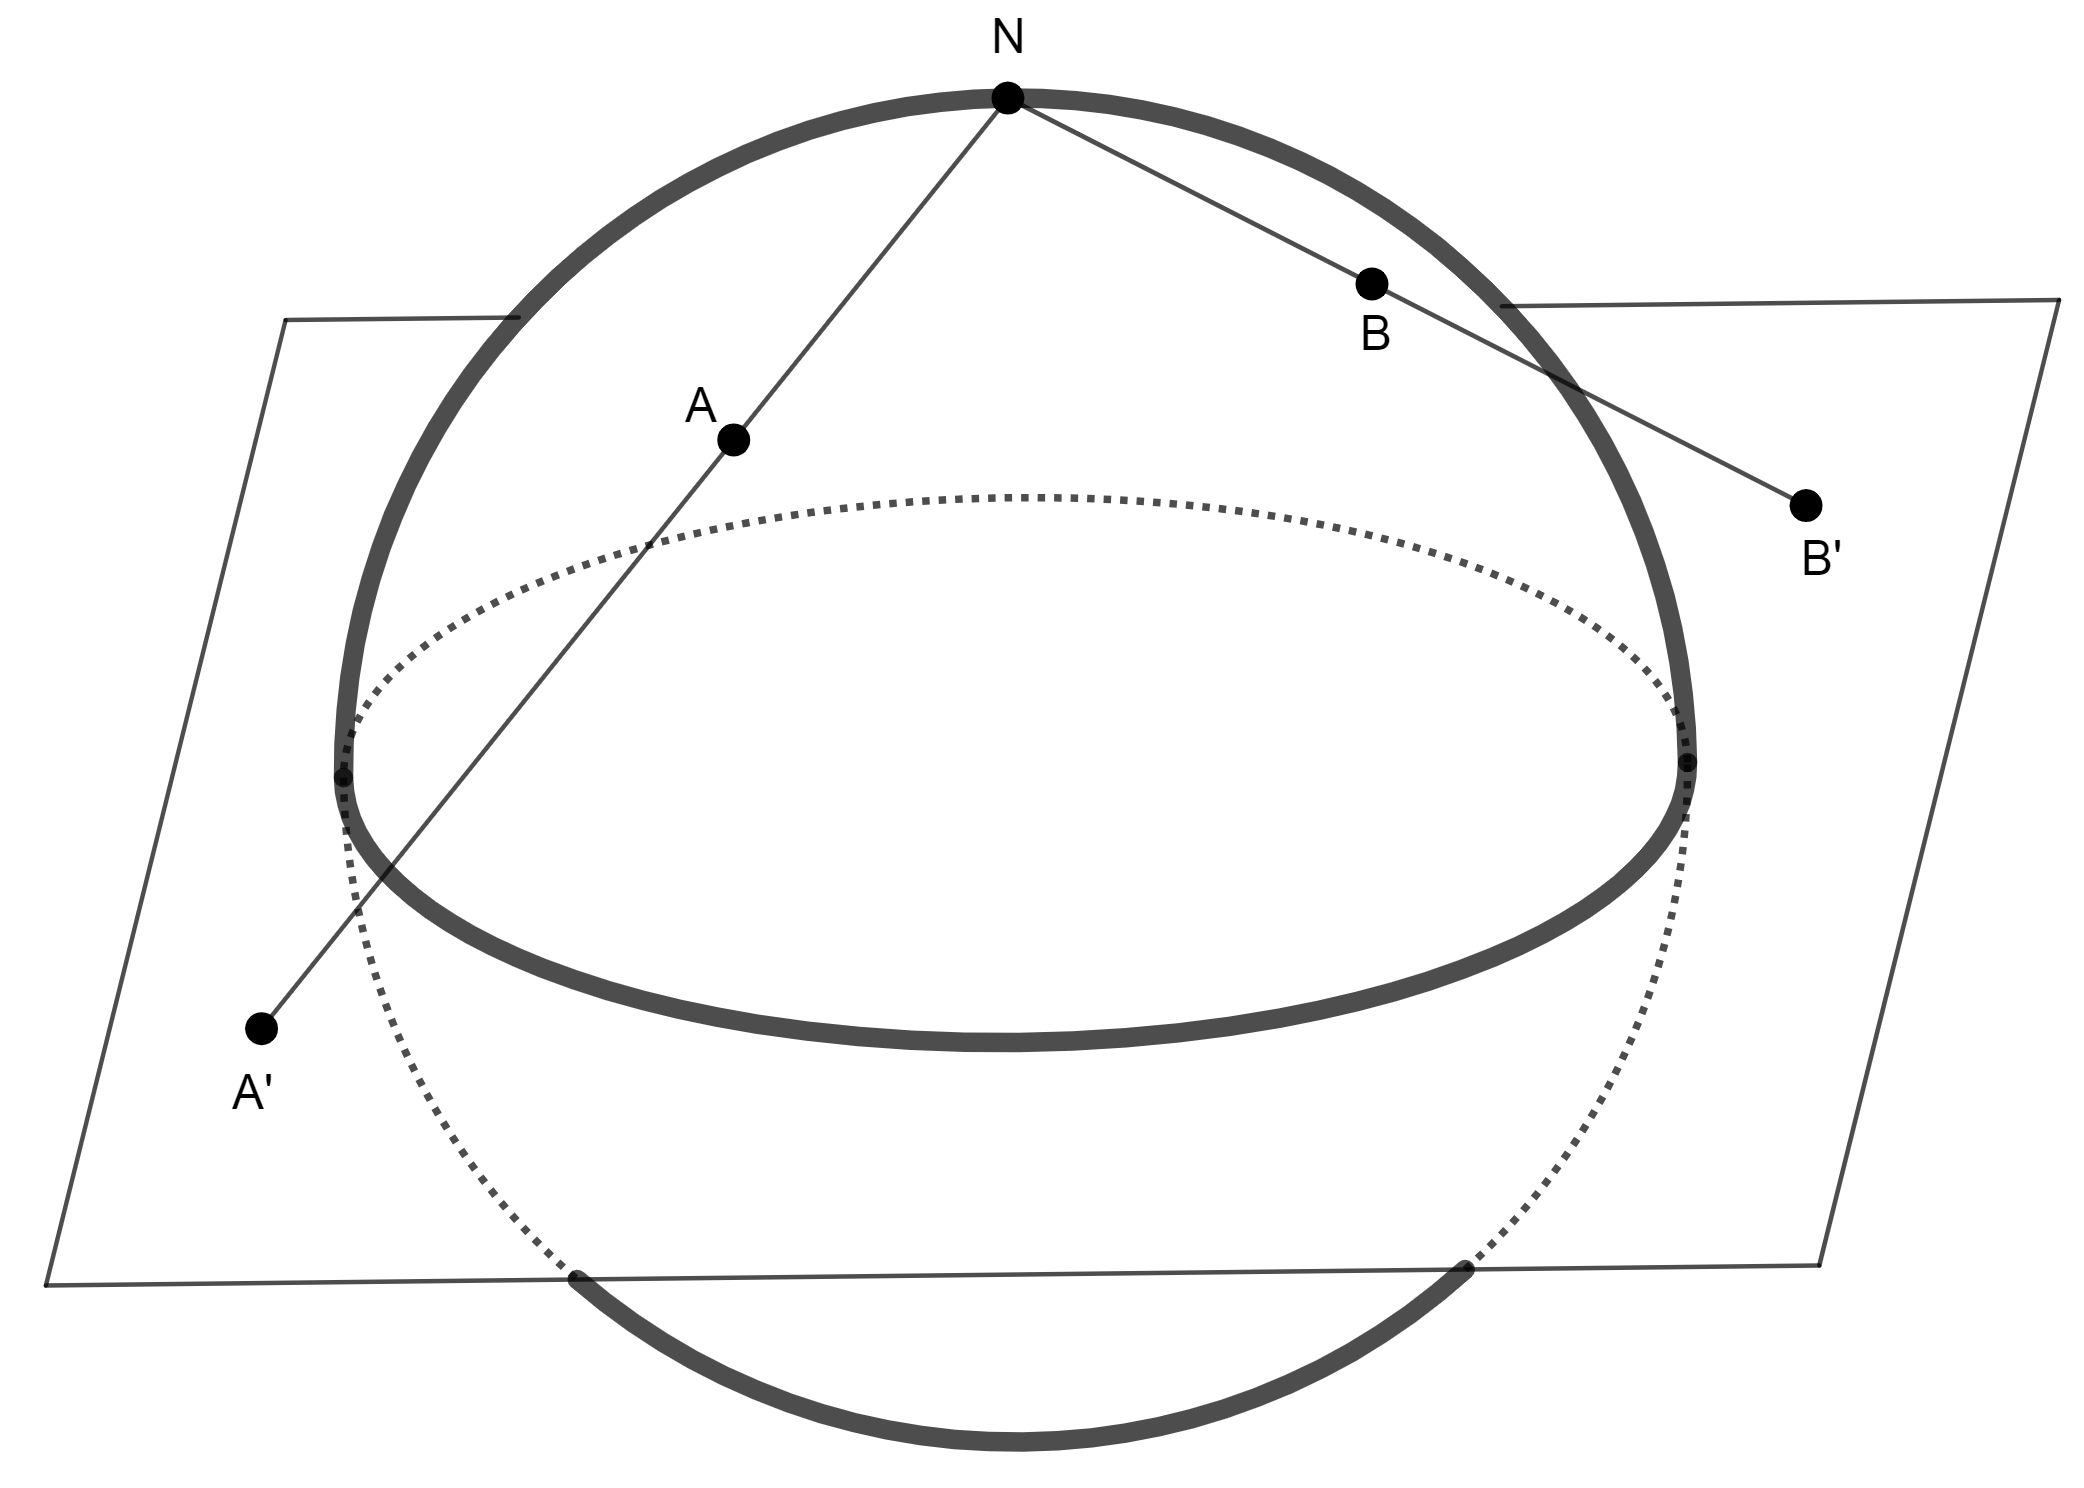
\includegraphics[width= 0.9\linewidth]{h2.png}
		\caption{\small\textit{\color{duongvaotoanhoc}Hình $2$: Qua phép chiếu lập thể, mặt cầu $\mathbb{S}^2$ bỏ đi điểm cực bắc $N$ trở thành mặt phẳng $\mathbb{R}^2$. Ta có thể xem $N$ như ``điểm ở xa vô tận'' của mặt phẳng.}}
		\vspace*{-10pt}
	\end{figure}
	Các đường cho ta bất biến đại số đầu tiên cho phép phân biệt các không gian tôpô (cho biết khi nào chúng không đồng phôi), được gọi là {\bf\color{duongvaotoanhoc} nhóm cơ bản}, định nghĩa bởi Henri Poincaré năm $1895$. Ta hãy cố định một điểm $x \in X$ và xét các đường từ $x$ đến chính nó, được gọi là các {\bf\color{duongvaotoanhoc} khuyên}. Ta xây dựng một phép toán trên chúng: cho $f$ và $g$ là hai khuyên tại $x$, ta định nghĩa $g \ast f: I \to X$ là khuyên thu được bằng cách đi theo $f$ với vận tốc gấp đôi rồi đi theo $g$ với vận tốc gấp đôi. Bằng công thức, 
	\begin{align*}
		(g \ast f)(t) \begin{cases}
			= f(2t) & \text{nếu } 0 \le t \le \frac{1}{2} \\
			= g(2t-1) & \text{nếu } \frac{1}{2} \le t \le 1.
		\end{cases}
	\end{align*}
	Như một thủ tục, ta cần kiểm tra các tiên đề của nhóm. Đầu tiên là tính kết hợp. Bằng tính toán trực tiếp, ta thấy ngay $h \ast (g \ast f) \neq (h \ast g) \ast f$. Tuy nhiên, hai đường này đồng luân. Điều này gợi ý rằng ta cần xem hai đường là như nhau nếu chúng đồng luân.
	\begin{figure}[H]
		\vspace*{5pt}
		\centering
		\captionsetup{labelformat= empty, justification=centering}
		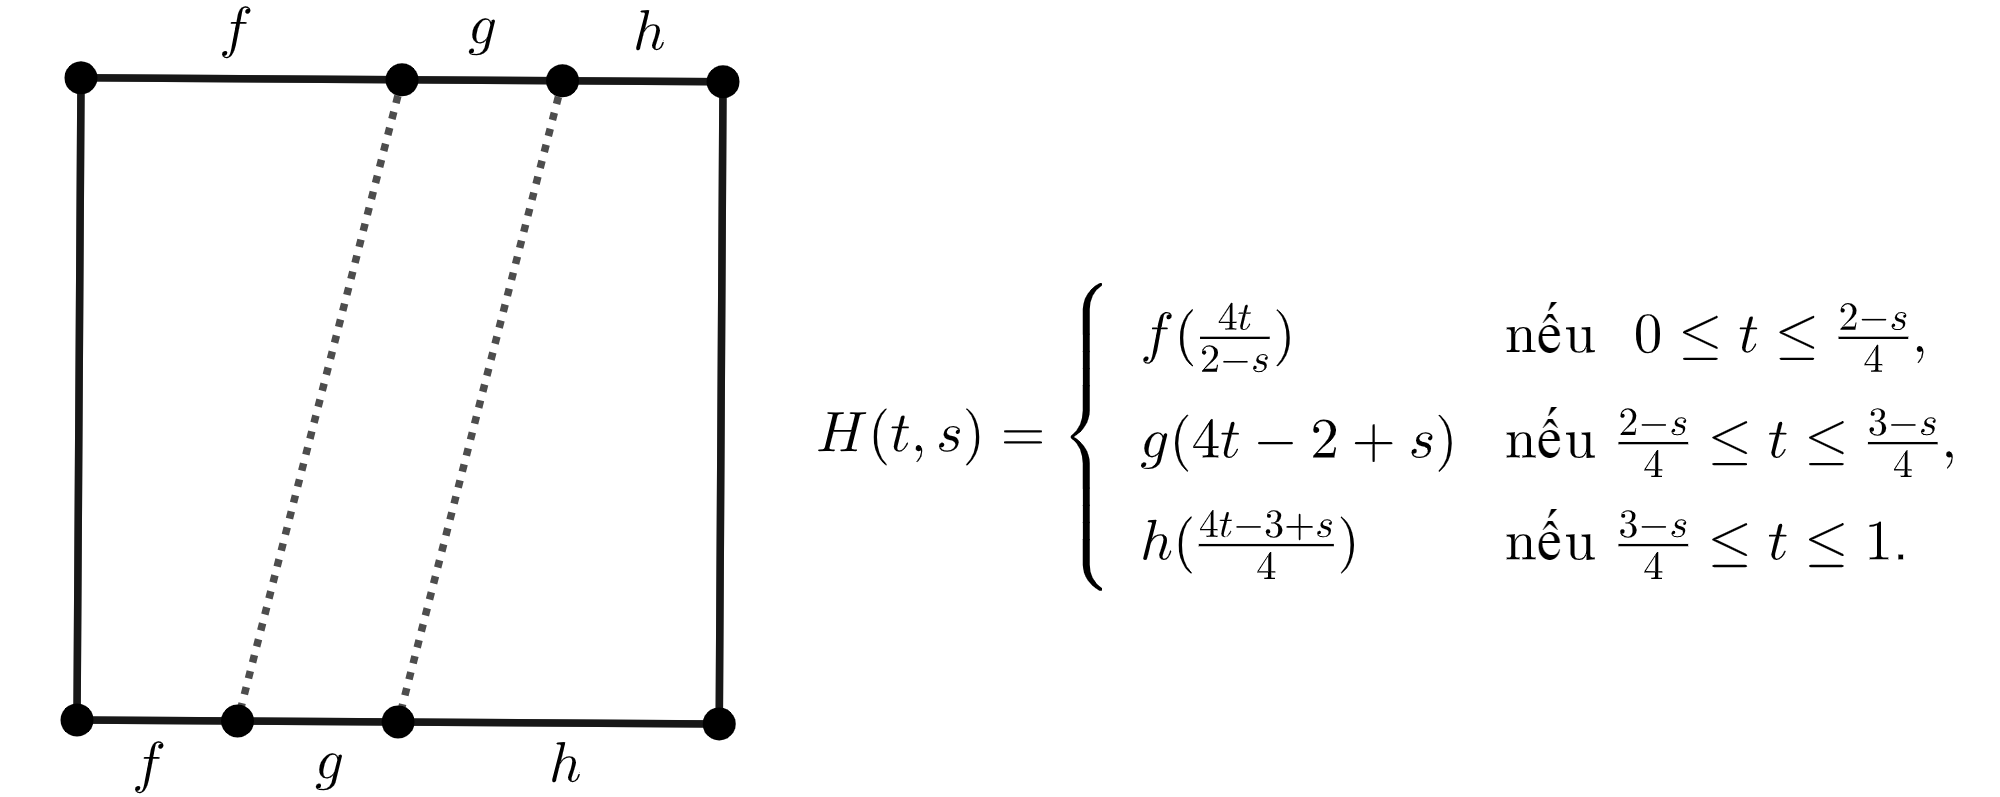
\includegraphics[width= 0.9\linewidth]{h3.png}
		\caption{\small\textit{\color{duongvaotoanhoc}Hình $3$: $h \ast (g \ast f) \sim (h \ast g) \ast f$.}}
		\vspace*{-10pt}
	\end{figure}
	Thứ hai, ta cần chỉ ra phần tử trung lập. Một cách trực giác, ta thấy nó phải là đường hằng $c$, cho bởi ``đứng yên tại $x$'', hay $c(t) = x$.
	\begin{figure}[H]
		\vspace*{-5pt}
		\centering
		\captionsetup{labelformat= empty, justification=centering}
		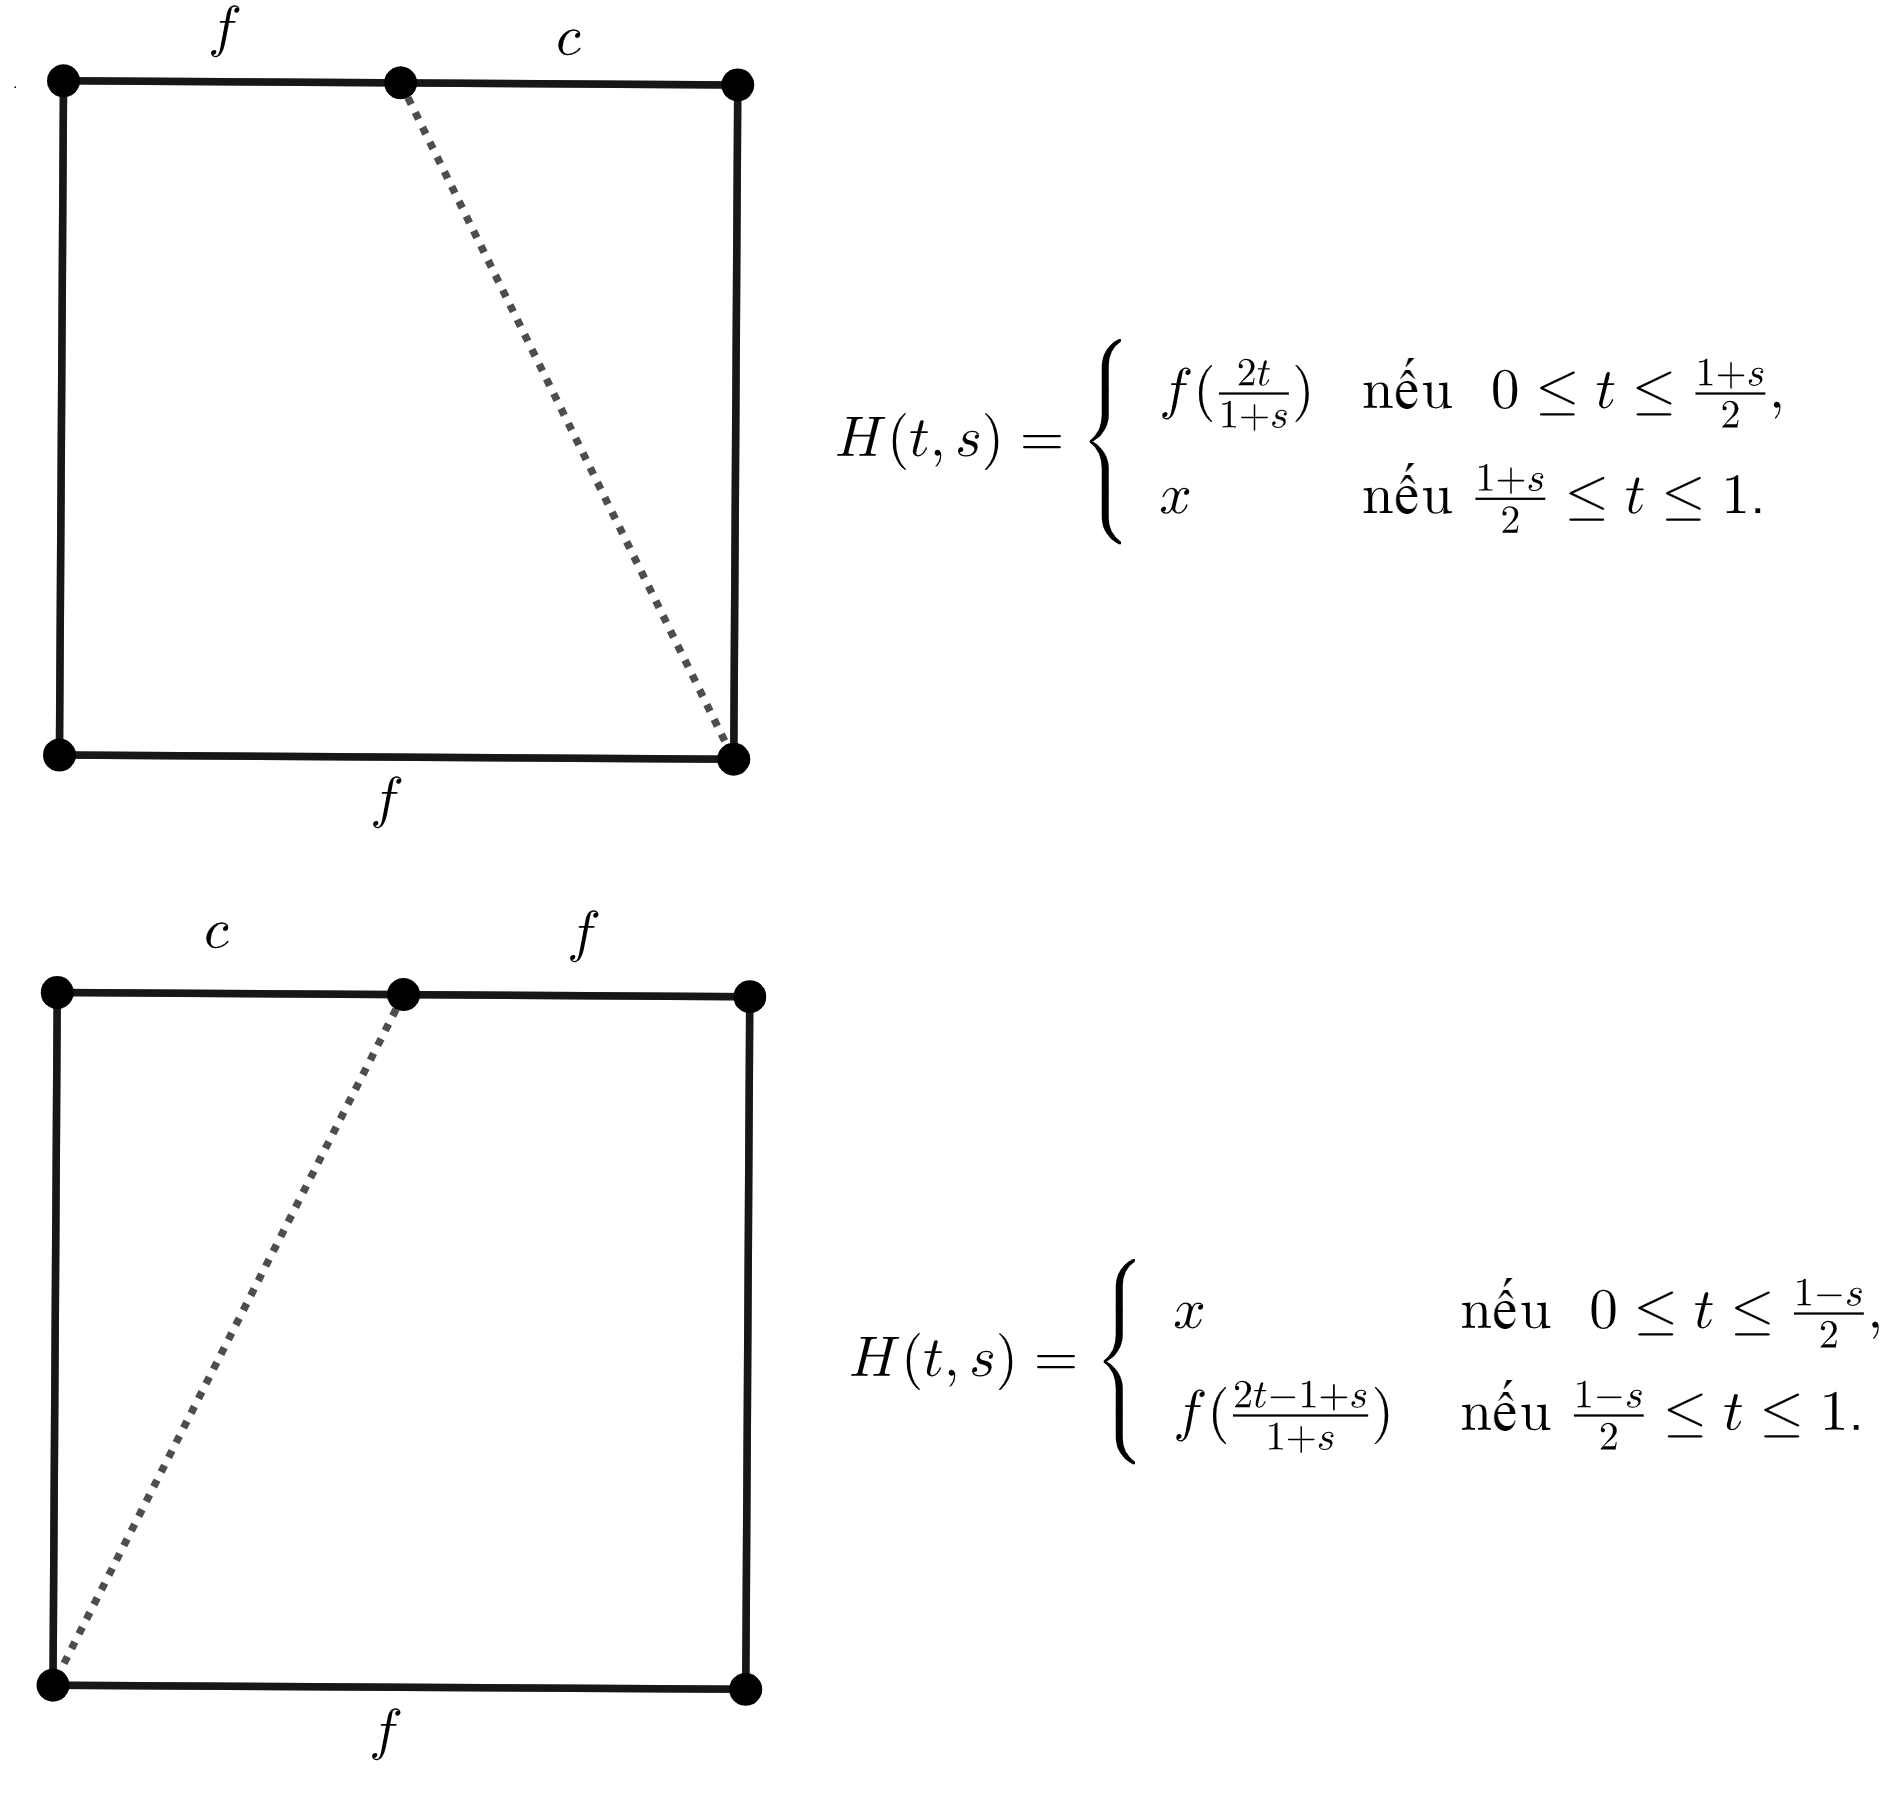
\includegraphics[width= 0.9\linewidth]{h4.png}
		\caption{\small\textit{\color{duongvaotoanhoc}Hình $4$: $f \ast c \sim f$ và $c \ast f \sim f$.}}
		\vspace*{-10pt}
	\end{figure}
	Cuối cùng, ta cần tìm nghịch đảo của một đường $f$ cho trước. Đó là đường $f'$ cho bởi ``đi ngược với $f$'', hay $f'(t) = f(1-t)$.
	\begin{figure}[H]
		\vspace*{-5pt}
		\centering
		\captionsetup{labelformat= empty, justification=centering}
		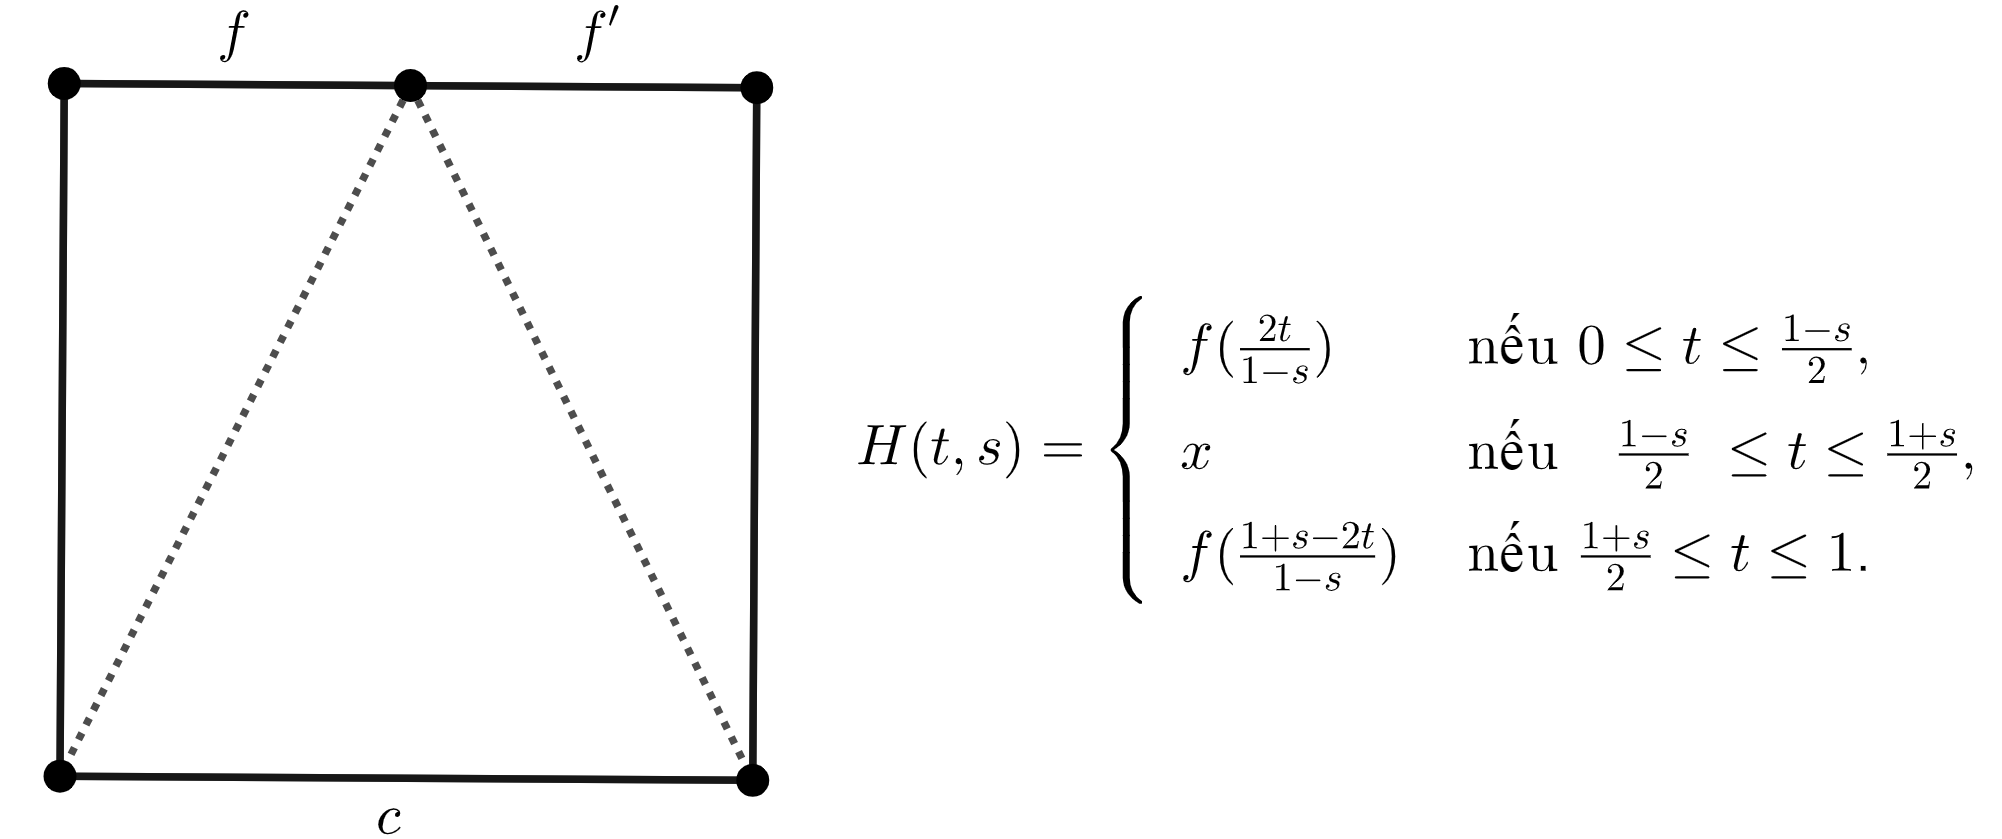
\includegraphics[width= 0.9\linewidth]{h5.png}
		\caption{\small\textit{\color{duongvaotoanhoc}Hình $5$: $f \ast f' \sim c$. Tất nhiên, vì $f'' = f$ nên $f' \ast f \sim c$.}}
		\vspace*{-10pt}
	\end{figure}
	Vậy các khuyên tại $x$ (sai khác đồng luân) tạo thành một nhóm, nó được gọi là nhóm cơ bản của $X$, ký hiệu bởi $\pi_1(X)$.
	\vskip 0.1cm
	Một không gian là đơn liên khi và chỉ khi nhóm cơ bản của nó tầm thường (mọi khuyên đều biến dạng liên tục được về một điểm). Chẳng hạn $\pi_1(\mathbb{R}^n) = 1$ và $\pi_1(\mathbb{S}^n) = 1$ với $n > 1$. Ví dụ không tầm thường đầu tiên là đường tròn $\mathbb{S}^1$, có thể xem như tập các số phức với môđun bằng $1$. Nhóm cơ bản của nó là (đẳng cấu với) $\mathbb{Z}$. Cụ thể, với mỗi số nguyên n, ta xét khuyên $f_n$ cho bởi $f_n(t) = \cos(2n \pi t)+i\cdot \sin(2n\pi t)$, đó là phép cuộn đoạn thẳng thành $|n|$ lần đường tròn (theo chiều dương nếu $n > 0$, theo chiều âm nếu $n < 0$). Một khuyên $f$ tùy ý đồng luân với $f_n$ khi và chỉ khi $f$ quay quanh đường tròn đúng $|n|$ lần với chiều tương ứng với dấu của $n$.
	\begin{figure}[H]
		\vspace*{-5pt}
		\centering
		\captionsetup{labelformat= empty, justification=centering}
		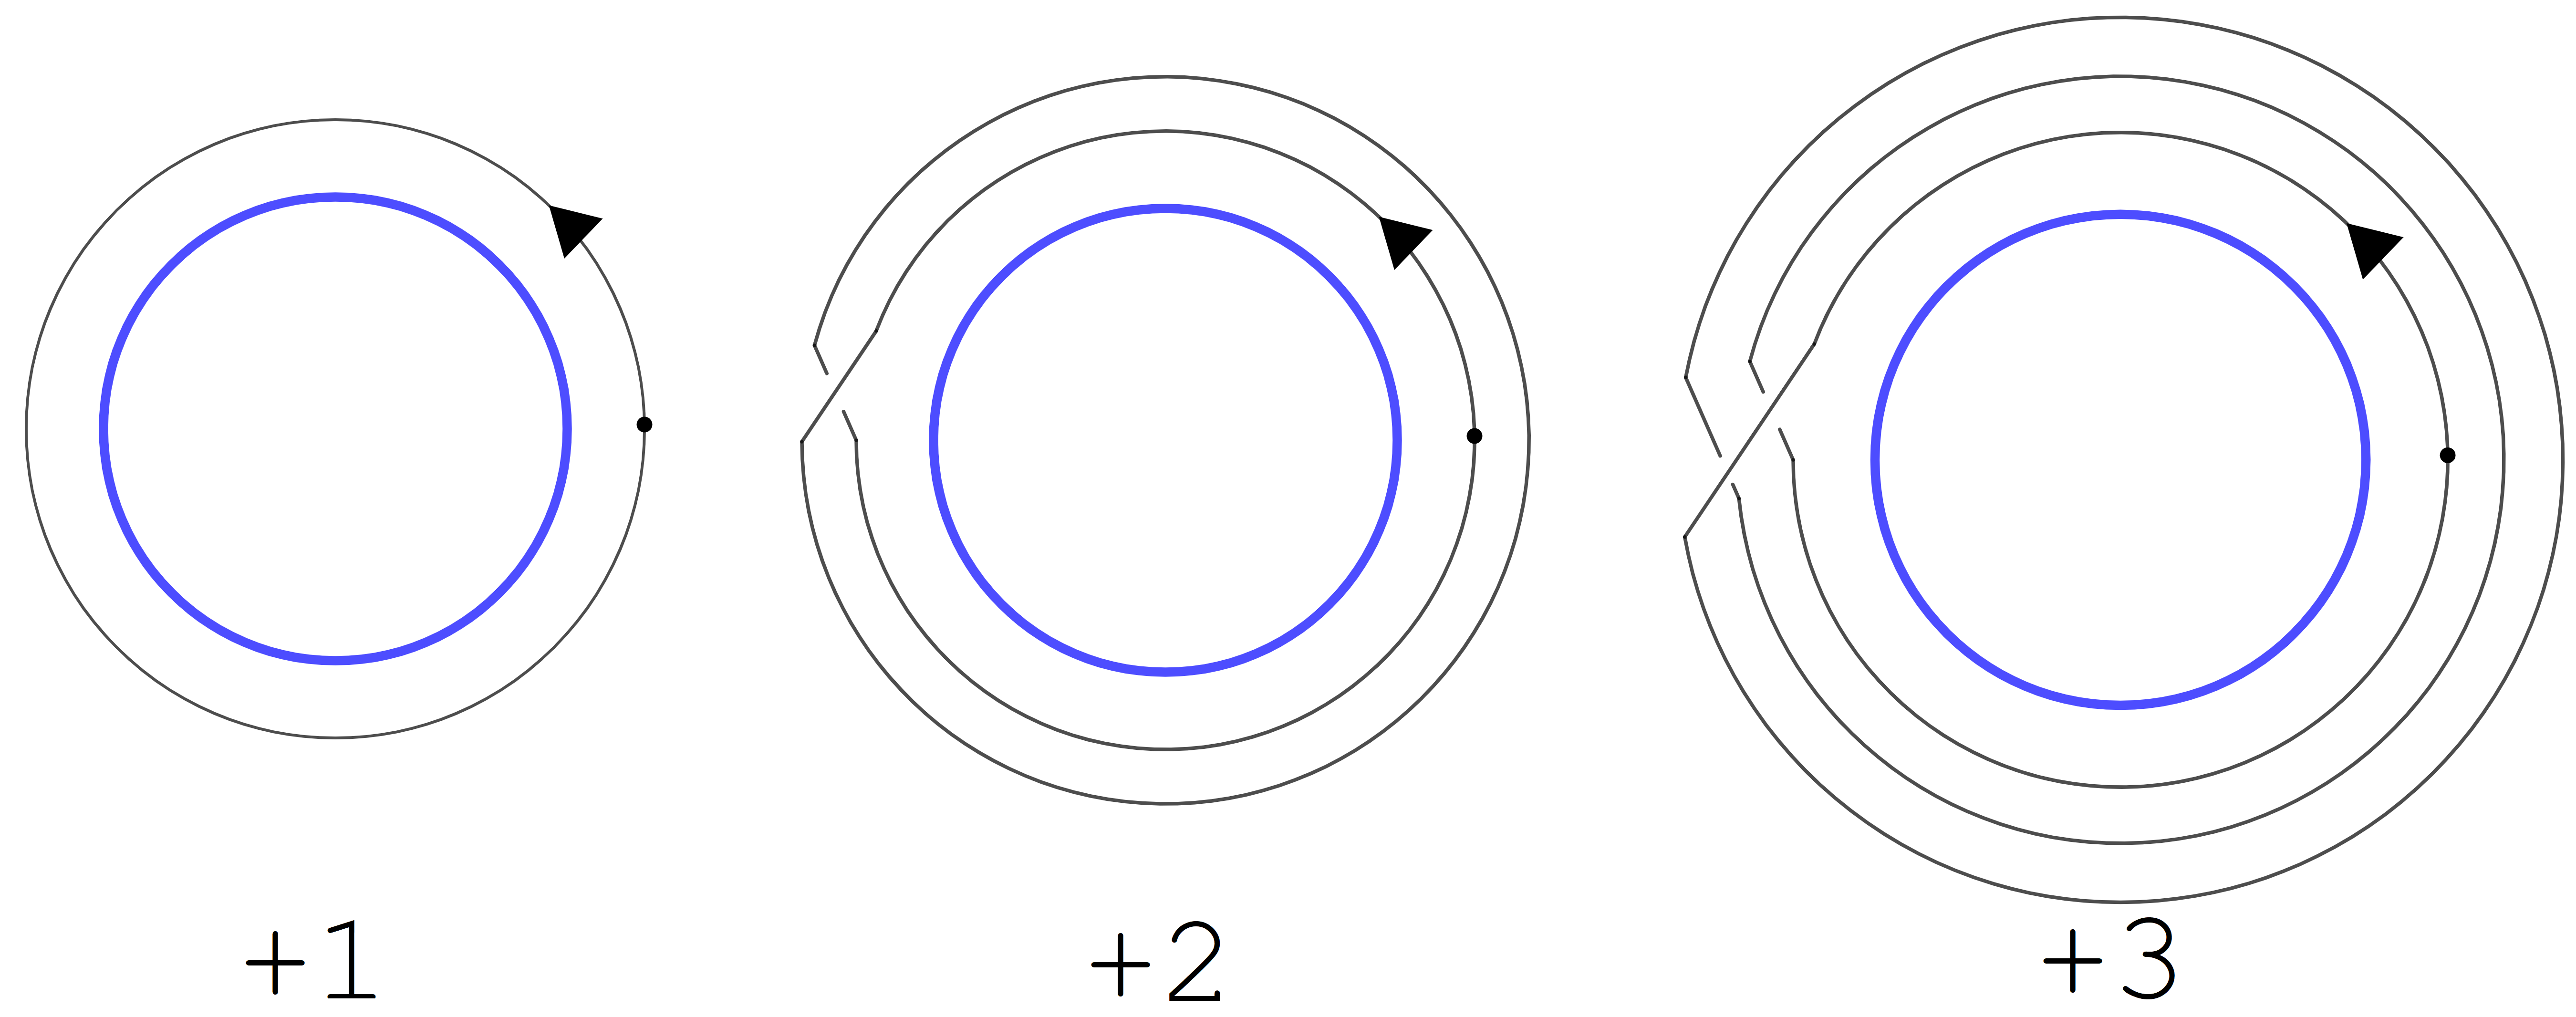
\includegraphics[width= 1\linewidth]{h6.png}
		\caption{\small\textit{\color{duongvaotoanhoc}Hình $6$: Nhóm cơ bản của đường tròn.}}
		\vspace*{-10pt}
	\end{figure}
	Cuối cùng, $f_n \ast f_m \sim f_{n+m}$, phép hợp thành của đường tương thích với phép cộng số nguyên, nghĩa là ta có đẳng cấu nhóm $\pi_1(\mathbb{S}^1) = \mathbb{Z}$.
	\vskip 0.1cm
	\textbf{\color{duongvaotoanhoc}Không gian phủ}
	\begin{figure}[H]
		\vspace*{-5pt}
		\centering
		\captionsetup{labelformat= empty, justification=centering}
		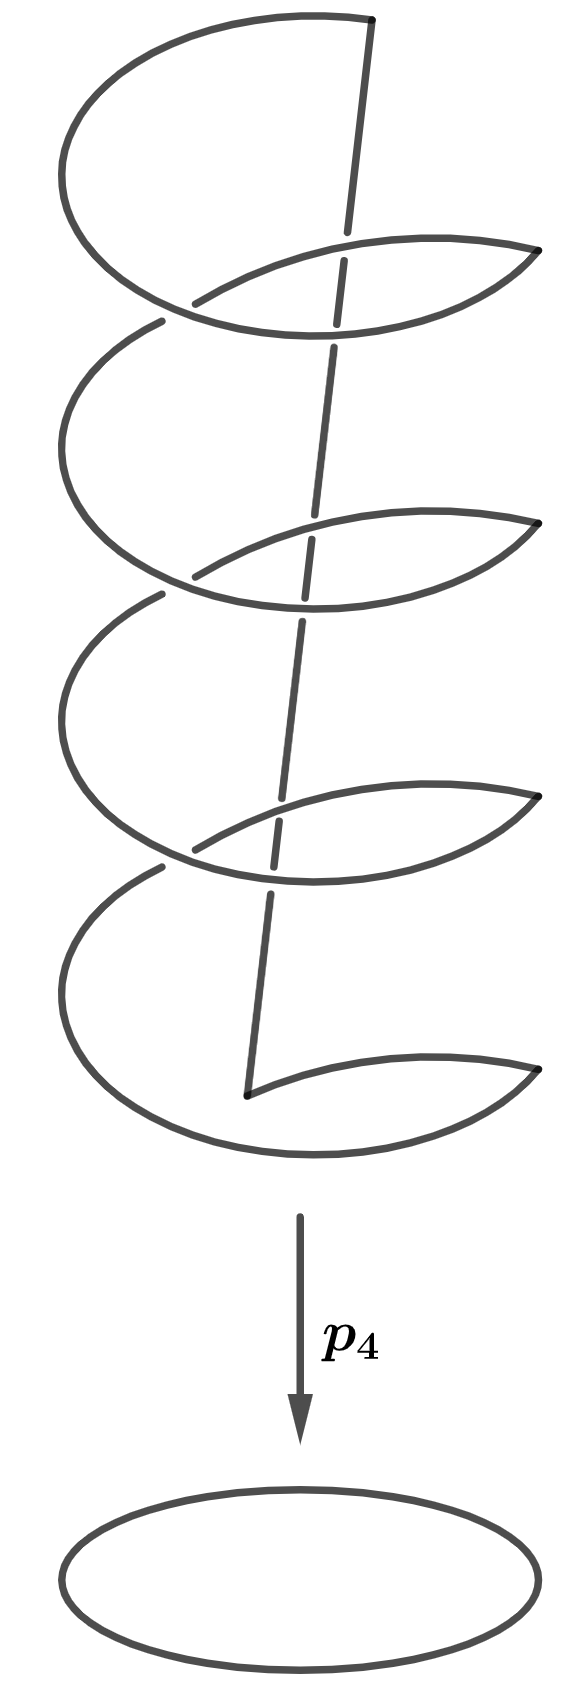
\includegraphics[width= 0.2\linewidth]{h7.png}
		\caption{\small\textit{\color{duongvaotoanhoc}Hình $7$: Đường tròn là một phủ $4$--tờ của chính nó.}}
		\vspace*{-10pt}
	\end{figure}
	Khái niệm gắn liền với nhóm cơ bản là {\bf\color{duongvaotoanhoc} không gian phủ}. Chẳng hạn, cho số nguyên dương $n$ và xét hàm liên tục $p_n: \mathbb{S}^1 \to \mathbb{S}^1$ cho bởi $p_n(z) = z^n$. Với mỗi điểm $w \in \mathbb{S}^1$, các điểm được $p_n$ biến thành $w$ (các căn bậc $n$ của $w$) tạo thành {\bf\color{duongvaotoanhoc} thớ} của $p_n$ tại $w$. Thớ này gồm $n$ điểm rời rạc. Hơn nữa, nếu ta chọn một lân cận $U$ đủ nhỏ quanh $w$ thì thớ của $U$ gồm $n$ thành phần liên thông rời nhau, mỗi thành phần này là một bản sao của U (cụ thể là $p_n$ cảm sinh một phép đồng phôi từ mỗi thành phần này lên $U$). Ta gọi một đó là một {\bf\color{duongvaotoanhoc} phủ $n$--tờ} hay {\bf\color{duongvaotoanhoc} phủ bậc $n$}. 
	\vskip 0.1cm
	Tổng quát, một phủ của không gian tôpô $X$ được cho bởi một không gian tôpô $Y$ cùng một hàm liên tục $p: Y \to X$ (ta coi $X$ là {\bf\color{duongvaotoanhoc} không gian nền} nằm dưới, $Y$ là {\bf\color{duongvaotoanhoc} không gian toàn phần} nằm trên), sao cho mỗi điểm của $X$ đều có một lân cận mà thớ được tạo thành từ một số (có thể vô hạn) bản sao rời rạc. Đây là một điều kiện hoàn toàn địa phương và từ nó không suy ra rằng bản thân $Y$ gồm các bản sao rời rạc của $X$.
		\begin{figure}[H]
		\vspace*{-5pt}
		\centering
		\captionsetup{labelformat= empty, justification=centering}
		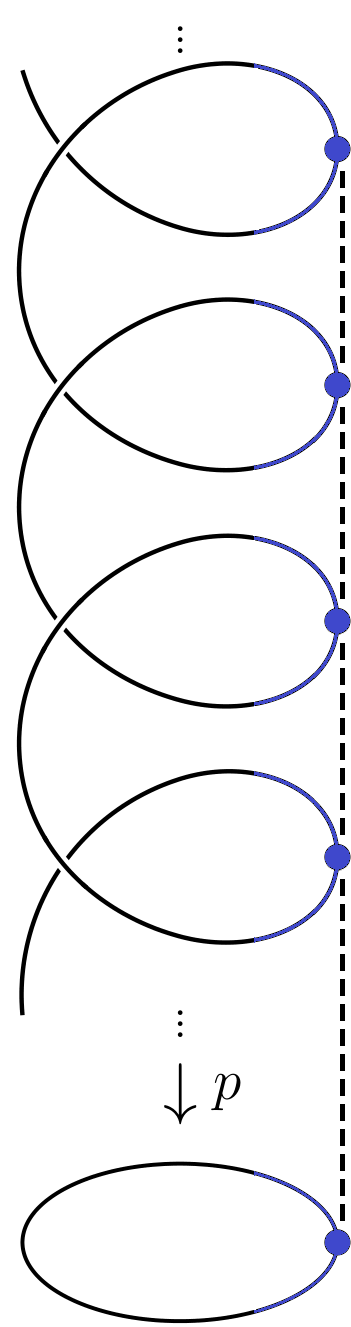
\includegraphics[width= 0.2\linewidth]{h8.png}
		\caption{\small\textit{\color{duongvaotoanhoc}Hình $8$: Phủ phổ dụng của đường tròn, cho bởi phép chiếu đường helix trong không gian $3$--chiều lên mặt phẳng. Mỗi điểm trên đường tròn đều có một lân cận mà thớ được tạo thành từ các bản sao rời rạc của chính lân cận đó.}}
		\vspace*{-5pt}
	\end{figure}
	Một ví dụ về phủ vô hạn tờ là $p: \mathbb{R} \to \mathbb{S}^1$ cho bởi $p(x) = \cos(2\pi x)+i \cdot \sin(2\pi x)$. Phủ này được gọi là {\bf\color{duongvaotoanhoc} phủ phổ dụng} của $\mathbb{S}^1$. Tại sao? Vì thông tin của nhóm cơ bản được thể hiện hoàn toàn trên nó. Một tính chất cơ bản của không gian phủ là tính nâng đường: cho một điểm $z \in \mathbb{S}^1$ và một điểm $x$ trên thớ của $z$, tức là $p(x) = z$. Với một đường bất kỳ $f: I \to \mathbb{S}^1$ xuất phát từ $z$, ta có thể {\bf\color{duongvaotoanhoc} nâng} nó thành một đường {\it duy nhất} $g: I \to \mathbb{R}$ xuất phát từ $x$, nghĩa là $p(g(t)) = f(t)$ và $g(0) = x$. Chẳng hạn khi $f$ là một khuyên tại z (hay $f(0) = f(1) = z$) thì $g(1)$ cũng nằm trên thớ của $z$, điều này tương đương với việc $g(1) - g(0)$ là một số nguyên. Chênh lệch này này hóa ra chính là số vòng quay của khuyên $f$ quanh đường tròn! Đây được gọi là {\bf\color{duongvaotoanhoc} tác động đơn đạo} của nhóm cơ bản $\pi_1(\mathbb{S}^1)$ lên phủ phổ dụng.
	\begin{figure}[H]
		\vspace*{-5pt}
		\centering
		\captionsetup{labelformat= empty, justification=centering}
		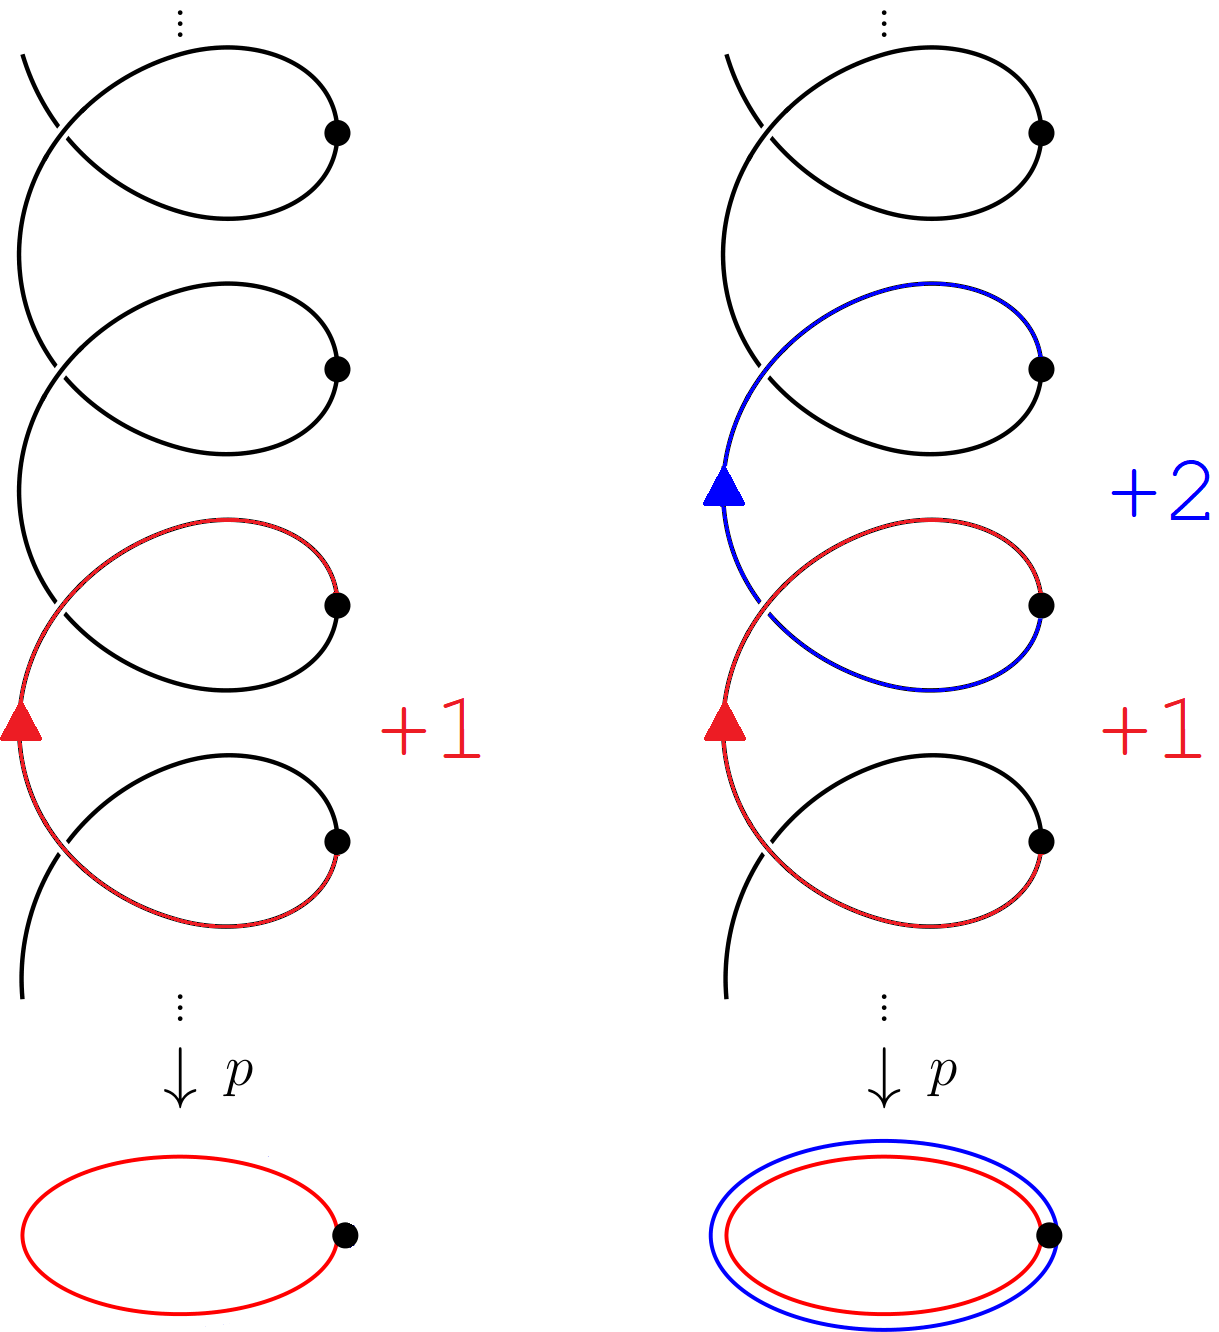
\includegraphics[width= 0.7\linewidth]{h9.png}
		\caption{\small\textit{\color{duongvaotoanhoc}Hình $9$: Tác động đơn đạo của nhóm cơ bản: khuyên $f_2(z) = z^2$ trên đường tròn được nâng thành phép tịnh tiến $g(x) = x+2$ trên phủ phổ dụng.}}
		\vspace*{-10pt}
	\end{figure}
	Như vậy, số vòng quay, vốn là một thông tin bị che mất nếu ta chỉ đơn thuần nhìn vào vết của đường trên không gian nền, đã được phục hồi khi ta nhìn vào không gian phủ.
	\vskip 0.1cm
	Định lý cơ bản của lý thuyết không gian phủ nói rằng có một tương ứng $1-1$ giữa các phủ (sai khác tương đương theo một nghĩa nào đó) với các nhóm con của nhóm cơ bản. Trong trường hợp đường tròn, các nhóm con của $\pi_1(\mathbb{S}^1) = \mathbb{Z}$ gồm $n\mathbb{Z}$ với $n$ nguyên dương (nhóm con các số nguyên chia hết cho $n$), cùng với $\{0\}$. Nhóm $n\mathbb{Z}$ có chỉ số $n$ trong $\mathbb{Z}$ (có $n$ lớp đồng dư modulo $n\mathbb{Z}$), nó ứng với phủ $n$-tờ $p_n: \mathbb{S}^1 \to \mathbb{S}^1$ cho bởi $p_n(z) = z^n$. Nhóm $\{0\}$ ứng với phủ phổ dụng $p: \mathbb{R} \to \mathbb{S}^1$, một phủ vô hạn tờ (và $\{0\}$ cũng có chỉ số vô hạn trong $\mathbb{Z}$). Và đó là tất cả. Nói riêng, với mỗi $n$, vì $\mathbb{Z}$ chỉ có đúng một nhóm con với chỉ số $n$ nên $\mathbb{S}^1$ chỉ có đúng một phủ $n$--tờ (sai khác tương đương).
	\vskip 0.1cm
	\textbf{\color{duongvaotoanhoc}Mở rộng trường}
	\vskip 0.1cm
	Lý thuyết về không gian phủ có một sự tương tự kỳ lạ với lý thuyết mở rộng trường của Galois. Để thấy phiên bản số học của đường tròn $\mathbb{S}^1$, ta quay lại với thế giới đại số. Một {\bf\color{duongvaotoanhoc} trường} là một tập hợp số mà ta có thể làm các phép toán cộng, trừ, nhân, chia. Chính xác hơn, ta có hai phép toán $+$ và $\times$ sao cho chúng thỏa mãn các tiên đề kết hợp, giao hoán, phân phối, có phần tử trung lập $0$, có phần tử đơn vị $1$, mọi ``số'' đều có số đối, và mọi số khác $0$ đều có nghịch đảo. Các ví dụ quen thuộc nhất là $\mathbb{Q}$, $\mathbb{R}$, $\mathbb{C}$. Trong khi đó, $\mathbb{Z}$ không phải một trường vì ta không thể làm phép chia $1 \div 2$ (sao kết quả vẫn nằm trong $\mathbb{Z}$).
	\vskip 0.1cm
	Một thao tác ta có thể làm với các trường là {\bf\color{duongvaotoanhoc} mở rộng}: ta kết nạp thêm nghiệm của một đa thức vô nghiệm trong trường ban đầu, và xét tất cả biểu thức thu được bằng cách cộng, trừ, nhân chia với phần tử mới này. Chẳng hạn, ta biết rằng đa thức $x^2 - 2$ không có nghiệm trong $\mathbb{Q}$. Khi kết nạp số thực $\sqrt{2}$, ta thu được tập các số $a + b\sqrt{2}$ với $a,b \in \mathbb{Q}$. Giá trị tại $\sqrt{2}$ của mọi đa thức hệ số hữu tỷ đều có thể viết được dưới dạng này: ta chỉ cần làm phép chia Euclid cho đa thức $x^2 - 2$ (dư sẽ có dạng $a + bx$) rồi thay $x = \sqrt{2}$. Để làm phép chia cho một số $a+b\sqrt{2} \neq 0$, ta chỉ đơn giản làm phép nhân liên hợp với $a-b\sqrt{2}$, vì $a+b\sqrt{2} = \frac{a^2 - 2b^2}{a-b\sqrt{2}}$. 
	\vskip 0.1cm
	Một câu hỏi mà thoạt nhìn có vẻ lẩm cẩm là ``số $\sqrt{2}$ lấy từ đâu ra?''. Việc xây dựng số thực từ số hữu tỷ là một thao tác phức tạp và nặng tính giải tích (gần như không hề đại số chút nào). Nhưng nếu ta không quan tâm đến tất cả số thực và chỉ muốn ``cái gì đó bình phương lên bằng $2$'' thì sao? Các nhà đại số rất giỏi trong việc này, họ thêm một phần tử mới hoàn toàn hình thức và tuyên bố rằng nó là nghiệm của đa thức $x^2 - 2$, và ký hiệu nó bởi $\sqrt{2}$. Một kiểu ``lý sự cùn'': tôi chẳng quan tâm $\sqrt{2}$ đến từ đâu, tôi chỉ cần biết nó thỏa mãn $(\sqrt{2})^2 - 2$ = 0 và tôi cộng trừ nhân chia với nó cứ như thể chẳng có gì xảy ra vậy! Nếu để ý, ta sẽ thấy rằng một khi ta đã gọi một nghiệm là $\sqrt{2}$ thì nghiệm còn lại của $x^2 - 2$ là $-\sqrt{2}$ (đa thức bậc $2$ nên chỉ có hai nghiệm này). Theo phong cách của các nhà đại số thì hoàn toàn không có cách nào để phân biệt giữa $\sqrt{2}$ và $-\sqrt{2}$ hết. Cứ chỗ nào có $\sqrt{2}$ thì thay bởi $-\sqrt{2}$, các tính toán vẫn không thay đổi. Để phân biệt hai số này, ta cần một thao mới (so với cộng, trừ, nhân, chia) là {\it so sánh}. Biết rằng có có hai căn bậc hai của $2$ trong $\mathbb{R}$, ta sẽ tuyên bố rằng, số nào lớn hơn $0$ thì được gọi là $\sqrt{2}$. Tình trạng tương tự xảy ra khi ta kết nạp vào $\mathbb{R}$ số $i$ và tuyên bố rằng $i^2 + 1 = 0$, thứ mà ngày nay ta gọi là {\bf\color{duongvaotoanhoc} số ảo}. Lúc này, để phân biệt $i$ với $-i$, ta không thể so sánh các số phức được nữa, giải pháp duy nhất là chọn một trong hai căn bậc hai của $-1$ và gọi nó là~$i$.
	\vskip 0.1cm
	Tổng quát hơn, nếu $f$ là một đa thức bất khả quy bậc $n > 1$ với hệ số trong một trường $K$ nào đó thì $f$ không có nghiệm trong $K$ (nếu nó có nghiệm $\alpha \in K$ thì nó chia hết cho đa thức $x - \alpha$, trái với giả thiết bất khả quy). Ta tuyên bố một cách hình thức rằng $\alpha$ là một ``nghiệm nào đó'' của $f$ và kết nạp $\alpha$ vào $K$. Trường mới thu được, ký hiệu bởi $K(\alpha)$, gồm các tổng (hình thức) có dạng $a_0+a_1\alpha+\cdots+a_{n-1}\alpha^{n-1}$, với $a_i \in K$. Ta cộng và trừ chúng một cách hiển nhiên. Khi làm phép nhân, ta chỉ cần chú ý rằng $f(\alpha) = 0$, từ đó $\alpha^n$ cũng có dạng $a_0+a_1\alpha+\cdots+a_{n-1}\alpha^{n-1}$, suy rộng ra thì giá trị tại $\alpha$ của mọi đa thức (bậc tùy ý) với hệ số trong $K$ cũng có dạng này. Để làm phép chia cho một phần tử $a_0+a_1\alpha+\cdots+a_{n-1}\alpha^{n-1} \neq 0$, ta xét đa thức $g(x) a_0+a_1x+\cdots+a_{n-1}x^{n-1}$. Vì $g(x) \neq 0$ nên $g$ không thể chia hết cho $f$, hay $g$ và $f$ nguyên tố cùng nhau (giả thiết $f$ bất khả quy được dùng ở đây), nên thuật toán Bézout cho ta các đa thức $u$, $v$ sao cho $fu+gv=1$, suy ra $g(\alpha)v(\alpha) = 1$, hay $v(\alpha)$ chính là nghịch đảo cần tìm của $g(\alpha)$. Mở rộng trường $K(\alpha)/K$ được gọi là một {\bf\color{duongvaotoanhoc} mở rộng bậc $n$}.
	\vskip 0.1cm
	\textbf{\color{duongvaotoanhoc}Trường hữu hạn}
	\vskip 0.1cm
	Nếu ta xét tập hợp $\mathbb{Z}/n\mathbb{Z}$ các lớp đồng dư modulo $n$ với $n$ là số nguyên dương cho trước, ta có thể làm phép cộng và phép nhân trên chúng một cách hiển nhiên. Thế thì $\mathbb{Z}/n\mathbb{Z}$ là một trường khi và chỉ khi $n = p$ là một số nguyên tố. Ta ký hiệu $\mathbb{Z}/p\mathbb{Z}$ bởi $\mathbb{F}_p$, một trường có $p$ phần tử. Các trường hữu hạn tìm thấy những ứng dụng quan trọng trong lý thuyết bảo mật hiện đại. 
	\vskip 0.1cm
	Tạm gác lại các ứng dụng của $\mathbb{F}_p$ trong tin học, ta hãy xem chúng có liên hệ gì với tôpô. Ta áp dụng phép mở rộng trường cho trường $\mathbb{F}_p$. Một suy luận đếm bằng hàm sinh và công thức nghịch đảo M\"obius đảm bảo rằng với mỗi số nguyên dương $n$, luôn tồn tại một đa thức $f$ với hệ số trong $\mathbb{F}_p$, bậc $n$, và bất khả quy. Kết nạp một nghiệm hình thức $\alpha$ của $f$ vào $\mathbb{F}_p$, ta thu được trường mới mà mỗi phần tử được viết duy nhất dưới dạng dạng $a_0+a_1\alpha+\cdots+a_{n-1}\alpha^{n-1}$, với $a_i \in \mathbb{F}_p$. Trường mới này vì thế có $p^n$ phần tử.
	\vskip 0.1cm
	Chẳng hạn, với $p = n = 2$, đa thức bậc $2$ bất khả quy duy nhất trên $\mathbb{F}_2$ là $x^2+x+1$. Ta tuyên bố rằng $\alpha$ là ``cái gì đó'' sao cho $\alpha^2 + \alpha + 1 = 0$ và kết nạp nó vào $\mathbb{F}_2$. Khi đó ta thu được một trường với $4$ phần tử là $0$, $1$, $\alpha$, $1 + \alpha$. Hai phần tử $\alpha$ và $1 + \alpha$ là nghịch đảo của nhau vì $\alpha(1 + \alpha) = \alpha^2 + \alpha = -1 = 1$ (ta đang xét modulo $2$!), từ đó ta có thể dễ dàng cộng, trừ, nhân, chia trên $4$ phần tử này.
	\vskip 0.1cm
	Trở lại với trường với $p^n$ phần tử, ta đã thấy rằng nó tồn tại. Ta muốn nó ``duy nhất'' theo nghĩa: hai trường có $p^n$ phần tử thì {\bf\color{duongvaotoanhoc} đẳng cấu} với nhau; một đẳng cấu trường là một tương ứng $1-1$ tương thích với các cấu trúc của trường (các phép toán cộng, trừ, nhân, chia, số $0$, số $1$). Trước hết, bằng một suy luận đại số tuyến tính đơn giản, mỗi trường hữu hạn $\mathbb{F}$ đều phải có số phần tử $q$ là lũy thừa của một số nguyên tố, $q = p^n$ chẳng hạn. Lúc này, $\mathbb{F}$ luôn ``chứa'' trường $\mathbb{F}_p$, theo nghĩa các phần tử $0,1,2 \ldots p-1$ trong $\mathbb{F}$ tạo thành một bản sao đẳng cấu với $\mathbb{F}_p$; ta cộng, trừ, nhân, chia chúng theo modulo $p$. Khi bỏ đi số $0$ khỏi $\mathbb{F}$, ta thu được một nhóm đối với phép nhân, một nhóm với $q-1$ phần tử. Định lý Lagrange trong lý thuyết nhóm đảm bảo rằng $a^{q-1} = 1$ với mọi $a \neq 0$, hay $a^q = a$ với mọi $a \in \mathbb{F}$. Đây là một tổng quát hóa của định lý nhỏ Fermat trong $\mathbb{F}_p$ (vì thực ra cách chứng minh cũng y hệt). Vậy, mọi phần tử của $\mathbb{F}$ đều là nghiệm của đa thức $x^q - x$, hay $\mathbb{F}$ thu được bằng cách kết nạp tất cả nghiệm của đa thức này vào $\mathbb{F}_p$. Lý thuyết mở rộng trường gọi $\mathbb{F}$ là (một) {\bf\color{duongvaotoanhoc} trường phân rã} của đa thức $x^q - x$, và nó đảm bảo rằng trường phân rã là duy nhất sai khác đẳng cấu. Như vậy, với mọi lũy thừa nguyên tố $p^n$, có duy nhất một trường với $p^n$ phần tử, một mở rộng bậc $n$ của $\mathbb{F}_p$.
	\vskip 0.1cm
	Tổng quát hơn, nếu $\mathbb{F}$ là một trường hữu hạn thì với mọi số nguyên dương $n$, tồn tại duy nhất (sai khác đẳng cấu) một mở rộng bậc $n$ của $\mathbb{F}$. Ta đã từng nói rằng lý thuyết không gian phủ có sự tương tự với lý thuyết mở rộng trường. Hãy nghĩ về các phủ $n$-tờ như các mở rộng bậc $n$. Vậy chẳng phải trường hữu hạn $\mathbb{F}$ rất giống đường tròn $\mathbb{S}^1$ ư? Dù trông nó như một sự tình cờ, ta hãy miễn cưỡng lấy quan sát này làm mở đầu cho sự liên hệ giữa tôpô và số học ở phần dưới. Sớm thôi, ta sẽ thấy rằng nó cũng không ngẫu nhiên lắm đâu.
	\vskip 0.1cm
	\textbf{\color{duongvaotoanhoc}Lược đồ}
	\vskip 0.1cm
	Bây giờ, hãy dạo qua thế giới hình học đại số một chút. Với ý tưởng tiên phong của Descartes là nghiên cứu các đối tượng hình học bằng các hệ tọa độ và phương trình đa thức, người ta đã dần dần phát triển hình học đại số. Khác với những người bạn bên tôpô học, các nhà hình học đại số nghiên cứu các đối tượng cứng nhắc hơn: tập nghiệm của các hệ phương trình đa thức. Sau một thời gian, giới toán học nhận ra rằng các trực giác hình học thường mang đến các chứng minh không chặt chẽ và đặc biệt là không giúp gì được ở số chiều cao hơn. Họ đã chuyển sang dùng đại số giao hoán làm công cụ chính để nghiên cứu hình học. Grothendieck, nhà toán học được công nhận rộng rãi là có ảnh hưởng nhất thế kỷ XX, đã cách mạng hóa hình học đại số một lần nữa bằng định nghĩa {\bf\color{duongvaotoanhoc} lược đồ}.
	\vskip 0.1cm
	Ta quay lại với khái niệm trường. Nếu bỏ qua việc luôn làm được phép chia, ta thu được khái niệm {\bf\color{duongvaotoanhoc} vành}. Chẳng hạn, $\mathbb{Z}$ và $\mathbb{Z}/n\mathbb{Z}$ là các vành (phép cộng và phép nhân được hiểu theo nghĩa hiển nhiên). Chú ý rằng ta vẫn yêu cầu làm được phép trừ, nên $\mathbb{N}$ không phải là một vành. Với mỗi vành $R$, ta xây dựng được một không gian tôpô $\text{Spec}(R)$, được gọi là {\bf\color{duongvaotoanhoc} phổ} của $R$. Nếu chỉ nhìn $\text{Spec}(R)$ như một không gian thì ta mất rất nhiều thông tin. Chẳng hạn, phổ của một trường luôn là một điểm. Vì thế, người ta đã làm giàu $\text{Spec}(R)$ một cấu trúc gọi là {\bf\color{duongvaotoanhoc} bó}, chúng làm cho $\text{Spec}(R)$ trở thành một lược đồ.
	\vskip 0.1cm
	Cũng như việc người ta quan tâm đến các hàm liên tục giữa các không gian tôpô, trong hình học đại số người ta quan tâm đến các {\bf\color{duongvaotoanhoc} cấu xạ} giữa các lược đồ. Một cấu xạ $\text{Spec}(R) \to \text{Spec}(S)$ đơn giản được cho bởi một {\bf\color{duongvaotoanhoc} đồng cấu vành} theo chiều ngược lại $f: S \to R$, đồng cấu ở đây nghĩa là $f(x+y) = f(x)+f(y)$, $f(xy) = f(x)f(y)$ và $f(1) = 1$. Chẳng hạn, $\mathbb{Z}$ là một vành con của $\mathbb{Q}$, và phép bao hàm $\mathbb{Z} \to \mathbb{Q}$ cho ta một cấu xạ $\text{Spec}(\mathbb{Q}) \to \text{Spec}(\mathbb{Z})$. Về mặt tôpô thì $\text{Spec}(\mathbb{Q})$ chỉ có một điểm, nên ảnh của cấu xạ này là một điểm của $\text{Spec}(\mathbb{Z})$, được gọi là {\bf\color{duongvaotoanhoc} điểm tổng quát}. Với mỗi số nguyên tố $p$, phép lấy dư modulo $p: \mathbb{Z} \to \mathbb{F}_p$ cho ta một cấu xạ $\text{Spec}(\mathbb{F}_p) \to \text{Spec}(\mathbb{Z})$, đó là một {\bf\color{duongvaotoanhoc} điểm đóng}. Các điểm đóng này và điểm tổng quát tạo nên không gian $\text{Spec}(\mathbb{Z})$. Khác với các không gian Euclid, tôpô trên lược đồ $\text{Spec}(\mathbb{Z})$ rất thô: điểm tổng quát là một điểm nhưng lại trù mật trong cả không gian (người ta hay nói ``điểm tổng quát là điểm nằm ở mọi nơi, nhưng không nằm cụ thể ở đâu cả'').
	\vskip 0.1cm
	Quay lại với lý thuyết không gian phủ. Khi áp dụng nó cho lược đồ, ta không thể chỉ xét khía cạnh tôpô ngây thơ được. Ta muốn $\text{Spec}(\mathbb{F}_p)$ giống với đường tròn $\mathbb{S}^1$, nhưng $\text{Spec}(\mathbb{F}_p)$ lại chỉ có một điểm. Vấn đề với không gian tôpô $\text{Spec}(R)$ là nó có quá ít lân cận, mỗi lân cận đều quá lớn. Cách khắc phục là sáng tạo ra một khái niệm tôpô mới dùng được cho các lược đồ (thứ mà ngày nay gọi là tôpô Grothendieck), với các ``lân cận'' mới. Một trong những loại tôpô đủ mạnh để phân biệt các ``không gian 1 điểm'' $\text{Spec}(K)$ (với $K$ là các trường) là {\bf\color{duongvaotoanhoc} tôpô étale}. Từ ``étale'' được lấy từ văn học Pháp, mang nghĩa nôm na là trạng thái dịu dàng của biển. Với công cụ mới này, người ta định nghĩa được khái niệm nhóm cơ bản étale của lược đồ. Chẳng hạn, nhóm cơ bản étale của $\text{Spec}(\mathbb{F}_p)$ là một nhóm có cùng họ hàng với $\mathbb{Z}$, gọi là ``$\mathbb{Z}$ mũ''. Điều này giải thích vì sao việc coi $\text{Spec}(\mathbb{F}_p)$ như đường tròn $\mathbb{S}^1$ là hợp lý. Tương tự, khái niệm phủ trong thế giới lược đồ phải được hiểu là phủ étale. Đối với các trường, một phủ étale của $\text{Spec}(K)$ đơn giản là $\text{Spec}(L)$, với $L/K$ là một mở rộng bậc hữu hạn. Như vậy, dù $\text{Spec}(K)$ về mặt tôpô chỉ một $1$ điểm, nó lại có nhóm cơ bản étale không tầm thường, hay có rất nhiều phủ. 
	\vskip 0.1cm
	Thực ra khái niệm mở rộng trường và mở rộng vành còn cho ta thêm một chút bên phía tôpô, nó ứng với khái niệm {\bf\color{duongvaotoanhoc} phủ phân nhánh}. Nói nôm na, một phủ phân nhánh bậc $n$ là một hàm liên tục $p: Y \to X$ sao cho nếu bỏ đi một số hữu hạn điểm của $X$ (và các điểm của $Y$ nằm trên chúng) thì ta thu được một phủ $n$-tờ. Các điểm bỏ đi kia (cùng các điểm nằm trên) gọi là các {\bf\color{duongvaotoanhoc} điểm rẽ nhánh} của $p$. Hiện tượng rẽ nhánh là phiên bản hình học của hiện tượng ``nghiệm bội'' trong đại số. Ta xét ví dụ khi $Y$ là đường cong elliptic cho bởi phương trình $y^2=x(x-1)(x-2)$ trong $\mathbb{C}^2$ và $X = \mathbb{C}$. Lấy $p$ là phép chiếu lên trục hoành, $p(x,y) = x$. Khi bỏ đi các điểm $0, 1, 2$ khỏi $X$ (và các điểm $(0,0), (1,0), (2,0)$ khỏi $Y$), ta thu được một phủ $2$--tờ: với mỗi $x \neq 0,1,2$ thì phương trình $y^2=x(x-1)(x-2)$ có hai nghiệm phức phân biệt. Ở các điểm $0, 1, 2$ xảy ra hiện tượng rẽ nhánh, phương trình $y^2=0$ có nghiệm kép $y=0$. Ta nói rằng {\bf\color{duongvaotoanhoc} chỉ số rẽ nhánh} của $p$ tại các điểm $(0,0)$, $(1,0)$, $(2,0)$ bằng $2$.
	\vskip 0.1cm
	\textbf{\color{duongvaotoanhoc}Lý thuyết số đại số}
	\vskip 0.1cm
	Để tìm hiểu các phủ (étale) phân nhánh của lược đồ $\text{Spec}(\mathbb{Z})$, ta bắt đầu từ điểm tổng quát: Phủ étale của $\text{Spec}(\mathbb{Q})$ thì có dạng $\text{Spec}(K)$, với $K = \mathbb{Q}(\alpha)$, và $\alpha$ là nghiệm của một đa thức bậc $n$ bất khả quy với hệ số hữu tỷ. Số $\alpha$ như vậy được gọi là một {\bf\color{duongvaotoanhoc} số đại số}, chẳng hạn $\sqrt{2}, \sqrt[3]{2}, \frac{1 + \sqrt{-3}}{2}$ là các số đại số. Trường $K$ được gọi là một {\bf\color{duongvaotoanhoc} trường số}, và mọi phần tử của nó đều là số đại số. Ta muốn thứ gì đó trong $K$ đóng vai trò như các số nguyên đối với số hữu tỷ. Đó là các {\bf\color{duongvaotoanhoc} số nguyên đại số}. Chúng là những phần tử của $K$ mà là nghiệm của một đa thức với hệ số nguyên và hệ số đầu bằng $1$. Chẳng hạn $\sqrt{2}$ là một số đại số vì nó là nghiệm của $x^2 - 2$. $\frac{1 + \sqrt{5}}{2}$ cũng là một số nguyên đại số (dù trông không có vẻ vậy) vì nó là nghiệm của $x^2-x-1$. Các số nguyên đại số trong $K$ tạo thành một vành $\mathcal{O}$. Việc chuyển từ $\mathbb{Z}$ sang $\mathcal{O}$ là chuyển từ lý thuyết số sơ cấp sang lý thuyết số đại số. Một bài tập đơn giản (bằng cách dùng phân tích duy nhất ra thừa số nguyên tố) là: Các số nguyên đại số trong $\mathbb{Q}$ chính là các số nguyên theo nghĩa cổ điển.
	\vskip 0.1cm
	Lý thuyết số đại số xuất phát từ nỗ lực chứng minh định lý lớn Fermat của Cauchy, Lamé... Ý tưởng như sau: với phương trình $x^2 + y^2 = z^2$ chẳng hạn, ta giải bằng cách đưa về $x^2=z^2-y^2=(z-y)(z+y)$, sau đó lập luận (với phân tích duy nhất ra thừa số nguyên tố) rằng $z-y$ và $z+y$ phải là các số chính phương. Bây giờ, xét phương trình $x^p+y^p=z^p$, với p là số nguyên tố lẻ (dễ thấy ta chỉ cần xét trường hợp này). Để phân tích triệt để $z^p-y^p$ thành các nhân tử bậc nhất, ta buộc phải dùng căn bậc $p$ phức của $1$. Gọi nó là $\zeta = \cos(\frac{2\pi}{p})+i \cdot \sin(\frac{2\pi}{p})$. Thế thì $\zeta$ là một số nguyên đại số (nghiệm của phương trình $x^p - 1$). Và như vậy ta đưa về chứng minh rằng phương trình trên không có nghiệm trong vành mới $\mathbb{Z}[\zeta]$, vành các số nguyên đại số của $\mathbb{Q}(\zeta)$. Sơ hở của cách tiếp cận này là lập luận như trong trường hợp $p=2$ không còn đúng nữa, vì nói chung không có phân tích duy nhất ra thừa số nguyên tố trong $\mathbb{Z}[\zeta]$.
	\vskip 0.1cm
	Một ví dụ về sự thiếu sốt của phân tích duy nhất là trường số $K = \mathbb{Q}(\sqrt{-5})$. Vành số nguyên đại số của nó là $\mathcal{O} = \mathbb{Z}[\sqrt{-5}]$, gồm các số có dạng $a+b\sqrt{-5}$ với $a,b \in \mathbb{Z}$. Số $6$ có thể phân tích thành $6 = 2 \cdot 3 = (1+\sqrt{-5}) \cdot (-\sqrt{-5})$. Để thấy rằng hai phân tích này là triệt để và thực sự khác nhau, ta định nghĩa {\bf\color{duongvaotoanhoc} chuẩn} của một số $a+b\sqrt{-5}$ bởi $N(a+b\sqrt{-5}) = a^2 + 5b^2$. Đây là một số tự nhiên, và ta thấy ngay rằng $N(xy) = N(x)N(y)$. Trong phân tích $6 = 2 \cdot 3 = (1+\sqrt{-5}) \cdot (-\sqrt{-5})$, ta có $N(2) = 4, N(3) = 9, N(1+\sqrt{-5}) = N(1-\sqrt{-5}) = 6$, nên các nhân tử xuất hiện ở hai phân tích thực sự khác nhau.  Ngoài ra, về cơ bản ta không thể phân tích thêm được nữa, vì không có phần tử nào có chuẩn bằng $2$ hoặc $3$ (một tính toán số học đơn giản cho thấy rằng phương trình các $a^2 + 5b^2 = 2$ và $a^2 + 5b^2 = 3$ đều không có nghiệm nguyên). Điều này cho thấy sự thiếu sót của phân tích duy nhất ra thừa số nguyên tố trong $\mathbb{Z}[\sqrt{-5}]$.
	\vskip 0.1cm
	Sự sụp đổ của phân tích duy nhất trong $\mathcal{O}$ đã chấm dứt hi vọng chứng minh định lý lớn Fermat bằng lý thuyết số đại số cổ điển. Dù vậy, vành $\mathcal{O}$ vẫn giữ được một tính chất của vành $\mathbb{Z}$; nó là một {\bf\color{duongvaotoanhoc} vành Dedekind}. Thay vì phân tích duy nhất của các số, người ta định nghĩa khái niệm {\bf\color{duongvaotoanhoc} số lý tưởng} (cái mà ngày nay gọi là {\bf\color{duongvaotoanhoc} iđêan}). Đại khái nó là thứ gì đó cho phép nói về quan hệ chia hết cũng như làm phép nhân. Việc $\mathcal{O}$ là vành Dedekind có nghĩa là mọi số lý tưởng đều phân tích một cách duy nhất ra các số lý tưởng nguyên tố. Một số nguyên đại số $a \in \mathcal{O}$ định nghĩa một số lý tưởng $(a)$, được gọi là một số lý tưởng chính. Hai số $a$ và $b$ định nghĩa cùng một số lý tưởng nếu chúng {\bf\color{duongvaotoanhoc} liên kết}, nghĩa là $a|b$ đồng thời $b|a$. Nói riêng, nếu là $u|1$ thì $(u) = (1)$. Nếu tất cả số lý tưởng nguyên tố đều có dạng trên thì $\mathcal{O}$ có phân tích duy nhất của các số (thực sự). Điều này không đúng trong $\mathbb{Z}[\sqrt{-5}]$; cụ thể là khi phân tích $(6) = (2) \cdot (3) = (1 + \sqrt{-5}) \cdot (1 - \sqrt{-5})$, ta vẫn phân tích được tiếp: $(2) = \mathfrak{p}_1\mathfrak{p}_2$, $(3) = \mathfrak{p}_3\mathfrak{p}_4$, $(1 + \sqrt{-5}) = \mathfrak{p}_1\mathfrak{p}_3$, $(1 - \sqrt{-5}) = \mathfrak{p}_2\mathfrak{p}_4$, trong đó $\mathfrak{p}_1, \mathfrak{p}_2, \mathfrak{p}_3, \mathfrak{p}_4$ là các số lý tưởng nguyên tố {\it không chính}. Chuẩn của chúng lần lượt là $N(\mathfrak{p}_1) = N(\mathfrak{p}_2) = 2$ và $N(\mathfrak{p}_3) = N(\mathfrak{p}_4) = 3$. Như vậy ta có phân tích duy nhất của $(6)$ thành các số lý tưởng.
	\vskip 0.1cm
	Cũng như mỗi số nguyên tố $p$ ứng với các điểm đóng $\text{Spec}(\mathbb{F}_p) \to \text{Spec}(\mathbb{Z})$, mỗi số lý tưởng nguyên tố $\mathfrak{p}$ trong trong $\mathcal{O}$ cho ta một trường hữu hạn $\mathbb{F}_{\mathfrak{p}}$ (gọi là {\bf\color{duongvaotoanhoc} trường thặng dư} của $\mathfrak{p}$), cùng một điểm đóng $\text{Spec}(\mathbb{F}_{\mathfrak{p}}) \to \text{Spec}(\mathcal{O})$. Cùng với điểm tổng quát $\text{Spec}(K)$, chúng tạo thành lược đồ $\text{Spec}(\mathcal{O})$. Vì $\mathbb{Z}$ là một vành con của $\mathcal{O}$, ta có một cấu xạ $\text{Spec}(\mathcal{O}) \to \text{Spec}(\mathbb{Z})$, một phủ étale phân nhánh. Mỗi số nguyên tố $p$ trong $\mathbb{Z}$ có thể không còn là số lý tưởng nguyên tố trong $\mathbb{O}$, nó phân rã thành tích của một số hữu hạn số lý tưởng nguyên tố, $(p) = \mathfrak{p_1}\mathfrak{p_2}\cdots\mathfrak{p_n}$. Các số lý tưởng nguyên tố xuất hiện trong phân tích trên chính xác là những điểm của $\text{Spec}(\mathcal{O})$ nằm trên điểm đóng của $\text{Spec}(\mathbb{Z})$ ứng với $p$. Hiện tượng phân nhánh nhánh xảy ra nếu có một số lý tưởng $\mathfrak{p}_i$ xuất hiện nhiều lần trong phân tích trên, ta gọi đó số lần đó là {\bf\color{duongvaotoanhoc} chỉ số rẽ nhánh} của $\mathfrak{p}_i$, nó đóng vai trò như chỉ số rẽ nhánh trong tôpô cổ điển.
	\vskip 0.1cm
	Một bất đẳng thức trong lý thuyết số đại số, {\it chặn Minkowski}, cho phép xác định cụ thể phân tích trên. Hơn thế nữa, nó còn cho ta biết chính xác khi nào thì một số nguyên tố $p$ rẽ nhánh trong $\mathcal{O}$. Một hệ quả của nó là với mọi trường số $K$, luôn có ít nhất một số nguyên tố $p$ rẽ nhánh trong vành $\mathcal{O}$ các số nguyên đại số trong $K$, nghĩa là $\text{Spec}(\mathbb{Z})$ không có phủ  étale không rẽ nhánh nào ngoài phủ tầm thường (cho bởi ánh xạ đồng nhất $\mathbb{Z} \to \mathbb{Z}$), hay nó là đơn liên.
	\vskip 0.1cm
	\textbf{\color{duongvaotoanhoc}Nút}
	\vskip 0.1cm
	Trong thế giới của các không gian tôpô thì có rất nhiều không gian đơn liên, và ta muốn tìm cái nào giống với $\text{Spec}(\mathbb{Z})$. Sự đột phá nằm ở các phát hiện sau đây của Mumford, Manin, và sau này là Mazur. Ở phía tôpô, các khái niệm điểm ($0$--chiều), đường ($1$--chiều), mặt ($2$--chiều) được tổng quát lên thành các đa tạp. Một đa tạp $3$--chiều là một không gian tôpô mà nhìn địa phương thì giống như không gian Euclid $\mathbb{R}^3$ (cũng như bề mặt trái đất là một đa tạp $2$--chiều, nhìn địa phương thì giống như mặt phẳng).
	\vskip 0.1cm
	Bên cạnh nhóm cơ bản, tôpô đại số cổ điển còn cung cấp các bất biến đại số khác cho các không gian tôpô, gọi là các {\bf\color{duongvaotoanhoc} nhóm đồng điều}. Nhóm đồng điều bậc $n$ của một đa tạp $X$ được xây dựng như sau: Xét các tổ hợp tạo thành từ một số đa tạp con $n$--chiều (chúng được gọi là các {\bf\color{duongvaotoanhoc} $n$-dây chuyền}). Nếu chúng tạo thành một vòng kín, ta gọi nó là một {\bf\color{duongvaotoanhoc} $n$--chu trình}. Nếu nó tạo thành biên của một đa tạp con $(n+1)$--chiều, ta gọi nó là một {\bf\color{duongvaotoanhoc} $n$--biên}. Một $n$--biên thì luôn là một $n$--chu trình. Nhóm $H_n(X)$ được định nghĩa là chênh lệch giữa các nhóm các $n$--chu trình và nhóm các $n$--biên: một $n$--chu trình mà không phải $n$--biên thì nó bao quanh một ``lỗ thủng'' $(n+1)$--chiều; như vậy các nhóm đồng điều phát hiện các lỗ thủng trên $X$. Phiên bản đối ngẫu của đồng điều là {\bf\color{duongvaotoanhoc} đối đồng điều}, các nhóm $H^n(X)$. Về cơ bản thì chúng cũng phát hiện các lỗ thủng. Về mặt kỹ thuật thì chúng dễ tính toán hơn đồng điều một chút, đồng thời có nhiều cấu trúc hơn. {\it Đối ngẫu Poincaré} nói rằng nếu $X$ là một đa tạp đóng, khả định hướng, $d$--chiều, thì ta có một đối ngẫu hoàn hảo giữa hai nhóm $H^{d-i}(X)$ và $H^i(X)$ với mỗi $i = 0,1,\ldots,d$.
	\vskip 0.1cm
	Với các lược đồ, các nhóm đối đồng điều nhìn chung không cho thông tin gì (phần lớn chúng bằng $0$) khi ta tính theo tôpô thông thường. Một lần nữa nhờ công của Grothendieck, ta có thể tính đối {\bf\color{duongvaotoanhoc} đồng điều étale}.  Trên một trường, chúng được gọi là đối {\bf\color{duongvaotoanhoc} đồng điều Galois}, một công cụ đã được dùng từ lâu trước đó trong số học. Với các trường hữu hạn, đối đồng điều Galois của chúng rất đơn giản, chúng khác $0$ ngoài bậc $0$ và $1$, và ta có một đối ngẫu hoàn hảo giữa các nhóm đối đồng điều ở hai bậc này. Điều này tương tự với đối ngẫu Poincaré cho các đa tạp $1$--chiều, khẳng định thêm niềm tin rằng phổ của trường hữu hạn là phiên bản đại số của đường tròn. 
	\vskip 0.1cm
	Đối với các lược đồ $\text{Spec}(\mathcal{O})$, với $\mathcal{O}$ là vành số nguyên đại số của một trường số $K$ nào đó, các nhóm đối đồng điều étale thỏa mãn đối ngẫu giữa bậc $0$ và bậc $3$ cũng như bậc $1$ và bậc $2$. Các kết quả này được gọi là {\it đối ngẫu Artin--Verdier}, được khám phá khi áp dụng đối đồng điều étale cho lý thuyết trường các lớp toàn cục, một phần của lý thuyết số. Điều này gợi cho ta rằng phiên bản tôpô của $\text{Spec}(\mathcal{O})$ ``nên" là các đa tạp $3$--chiều. Vậy $\text{Spec}(\mathbb{Z})$ ứng với đa đạp đóng $3$--chiều nào? Ta thấy ở trên rằng $\text{Spec}(\mathbb{Z})$ đơn liên, và đa tạp đóng $3$--chiều đơn liên thì chỉ có thể đồng phôi với mặt (siêu) cầu  $\mathbb{S}^3$! Đó là nội dung của {\it giả thuyết Poincaré}, bài toán duy nhất đã được giải trong $7$ bài toán thiên niên kỷ. Tác giả của lời giải, thiên tài lập dị Perelman, đã từ chối cả Huy chương Fields lẫn Giải Breakthrough cho công trình vô song của mình.
	\vskip 0.1cm
	Sau khi bỏ ra rất nhiều công sức, ta đã thấy được cầu nối mong manh giữa tôpô, rằng phiên bản số học của $\mathbb{S}^1$ là (phổ của) một trường hữu hạn, và của một đa tạp đóng $3$--chiều là vành các số nguyên đại số của một trường số. Bây giờ là lúc chúng ta thu hoạch kết quả, chiêm ngưỡng những sự tương tự đáng ngạc nhiên dựa trên cầu nối này. Một số lý tưởng nguyên tố $\mathfrak{p}$ trong $\mathcal{O}$ cho ta một phép nhúng $\text{Spec}(\mathbb{F}_\mathfrak{p}) \hookrightarrow \text{Spec}(\mathcal{O})$. Về phía tôpô, ta xét các phép nhúng $\mathbb{S}^1 \hookrightarrow M$, với $M$ là một đa tạp (đóng, khả định hướng) $3$-chiều. Chúng được gọi là các {\bf\color{duongvaotoanhoc} nút} trong $M$. Nói riêng, phiên bản tôpô của mỗi số nguyên tố $p$ (với phép nhúng tương ứng $\text{Spec}(\mathbb{F}_p) \hookrightarrow \text{Spec}(\mathbb{Z})$) là một nút trong $\mathbb{S}^3$ (ta sẽ tập trung vào các nút này). Từ một định lý sâu sắc trong tôpô học, {\it định lý Borsuk--Ulam}, ta có thể chỉ ra rằng một phép nhúng như thế không thể là toàn ánh, nghĩa là ta có thể xem một nút như một phép nhúng từ $\mathbb{S}^1$ vào $\mathbb{S}^3$ bỏ đi một điểm, nói cách khác chính là không gian Euclid $\mathbb{R}^3$.
	\vskip 0.1cm
	Để biểu diễn một nút $K: \mathbb{S}^1 \hookrightarrow \mathbb{R}^3$ ta có thể chiếu nó lên một mặt phẳng sau cho tại mỗi điểm giao nhau chỉ có đúng $2$ đường đi qua. Chúng ứng với một {\bf\color{duongvaotoanhoc} sợi trên} và một {\bf\color{duongvaotoanhoc} sợi dưới}, ta biểu diễn sợi dưới bằng nét đứt tại giao điểm đó.  Đó là một {\bf\color{duongvaotoanhoc} biểu đồ phẳng} của nút.
	\begin{figure}[H]
		\vspace*{-5pt}
		\centering
		\captionsetup{labelformat= empty, justification=centering}
		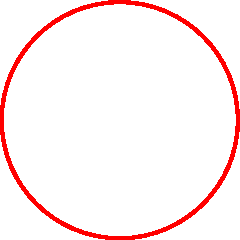
\includegraphics[width= 0.28\linewidth]{unknot.pdf}\quad
		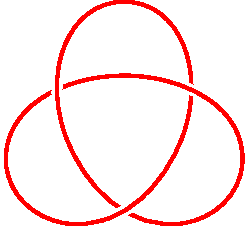
\includegraphics[width= 0.28\linewidth]{trefoil.pdf}\quad
		
\includegraphics[width= 0.28\linewidth]{figure 8.pdf}
		\caption{\small\textit{\color{duongvaotoanhoc}Hình $10$: Biểu đồ phẳng của nút tầm thường, nút ba lá, và nút số $8$.}}
		\vspace*{-10pt}
	\end{figure}
	Tất nhiên, mọi nút đều đồng phôi với $\mathbb{S}^1$. Ta cần cả thông tin về phép nhúng $\mathbb{S}^1 \to \mathbb{R}^3$ để phân biệt các nút với nhau. Các nhà lý thuyết nút gọi sự giống nhau của các nút là {\bf\color{duongvaotoanhoc} đẳng luân}. Một cách trực giác, hai nút đẳng luân nếu ta có thể tháo dỡ một nút rồi buộc thành nút còn lại (mà không cắt được cắt nút ra). Hóa ra, hai nút đẳng luân khi và chỉ khi phần bù của chúng trong $\mathbb{S}^3$ đồng phôi với nhau ({\it định lý Gordon--Luecke}).
	\vskip 0.1cm
	\textbf{\color{duongvaotoanhoc}Từ điển M$^2$KR}
	\vskip 0.1cm
	Từ điển Mazur--Morishita--Kapranov--Reznikov (M$^2$KR) là một danh sách những sự tương tự giữa lý thuyết số và hình học của các đa tạp $3$--chiều; ở đó các số lý tưởng tưởng ứng với các liên kết, các số lý tưởng nguyên tố ứng với các nút. Sau đây là một số tương ứng giữa tôpô và số học trong từ điển này.
	\vskip 0.1cm
	Mỗi số lý tưởng trong $\mathcal{O}$ phân tích thành tích của các số lý tưởng nguyên tố. Phiên bản tôpô của số lý tưởng là {\bf\color{duongvaotoanhoc} liên kết}: một liên kết trong một đa tạp đóng $3$--chiều $M$ là một phép nhúng từ một số hữu hạn bản sao rời rạc của $\mathbb{S}^1$ vào $M$. Các ví dụ về liên kết trong $\mathbb{S}^3$ là {\bf\color{duongvaotoanhoc} liên kết Hopf} và {\bf\color{duongvaotoanhoc} vòng Borromean}, lần lượt được tạo bởi $2$ và $3$ nút tầm thường lồng nhau.
	\begin{figure}[H]
		\vspace*{-15pt}
		\centering
		\captionsetup{labelformat= empty, justification=centering}
		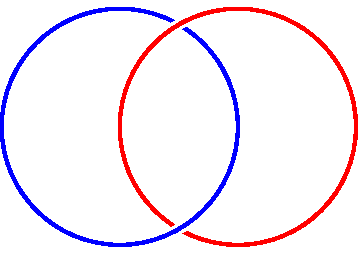
\includegraphics[width= 0.4\linewidth]{hopf.pdf}\quad\quad
		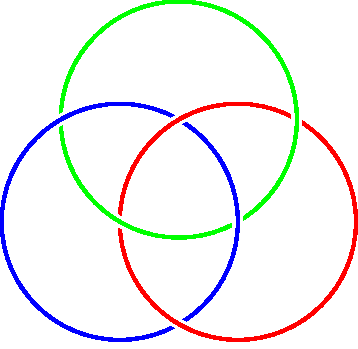
\includegraphics[width= 0.4\linewidth]{borromean.pdf}
		\caption{\small\textit{\color{duongvaotoanhoc}Hình $11$: Biểu đồ phẳng của liên kết Hopf và vòng Borromean.}}
		\vspace*{-10pt}
	\end{figure}
	Để thêm phần thuyết phục rằng tại sao $M$ lại tương ứng với (vành số nguyên đại số) một trường số, ta nhắc đến {\it định lý Alexander}: Mọi đa tạp đóng $3$--chiều đều là một phủ phân nhánh của $\mathbb{S}^3$, trong đó các điểm rẽ nhánh trong $\mathbb{S}^3$ tạo thành một liên kết. Tương tự, một mở rộng $L/K$ của trường số có thể được coi như một phủ phân nhánh giữa hai đa tạp đóng $3$--chiều.
	\vskip 0.1cm
	Một số nguyên đại số $a \in \mathcal{O}$ ứng với một mặt compact $S$ (có thể có biên) nhúng trong đa tạp đóng $3$--chiều $M$. Số lý tưởng chính $(a)$ ứng với biên $\partial S$, đây là một liên kết, và chúng ứng với các $1$--đối biên, tức là phần tử $0$ trong nhóm đồng điều $H_1(M)$. Các số lý tưởng khác tương ứng với các liên kết, chúng là các $1$--chu trình mà không phải biên, đại diện cho các phần tử không tầm thường của $H_1(M)$. Ta biết rằng trong $\mathbb{Z}$ có phân tích duy nhất ra thừa số nguyên tố, hay mọi số lý tưởng nguyên tố đều là số lý tưởng chính. Tương ứng, với $M = \mathbb{S}^3$, ta có $H_1(M) = 0$ (vì $\mathbb{S}^3$ không có lỗ thủng $2$--chiều nào), nghĩa là mọi liên kết đều là biên của một mặt nào đó. Seifert đã đưa ra một thuật toán khá đơn giản để xây dựng một mặt với biên cho trước. Chẳng hạn, {\bf\color{duongvaotoanhoc} mặt Seifert} của liên kết Hopf chính là {\it mặt M\"obius}.
	\begin{figure}[H]
		\vspace*{-5pt}
		\centering
		\captionsetup{labelformat= empty, justification=centering}
		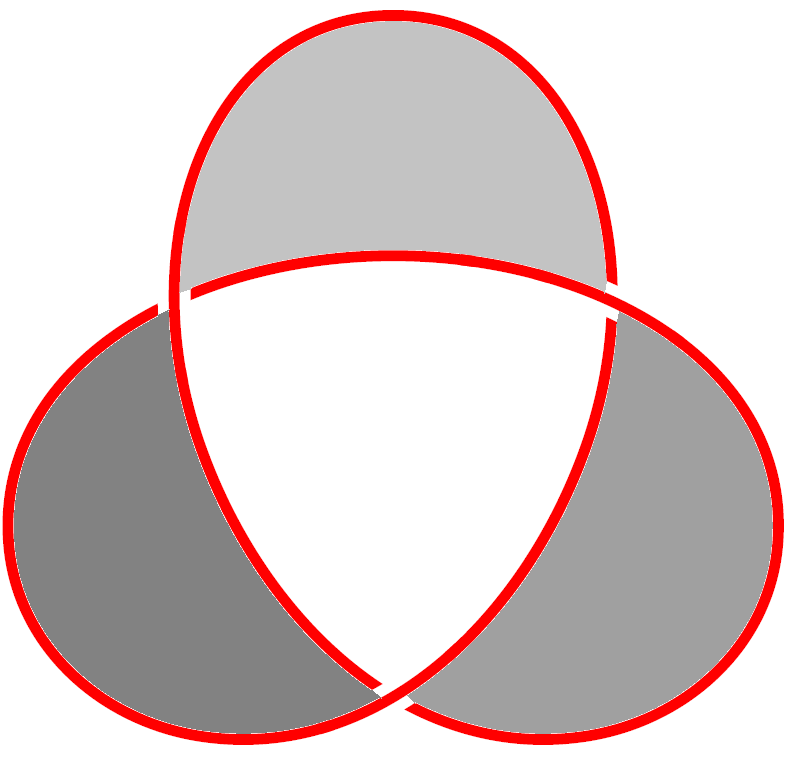
\includegraphics[width= 0.4\linewidth]{seifert1}\quad\quad
		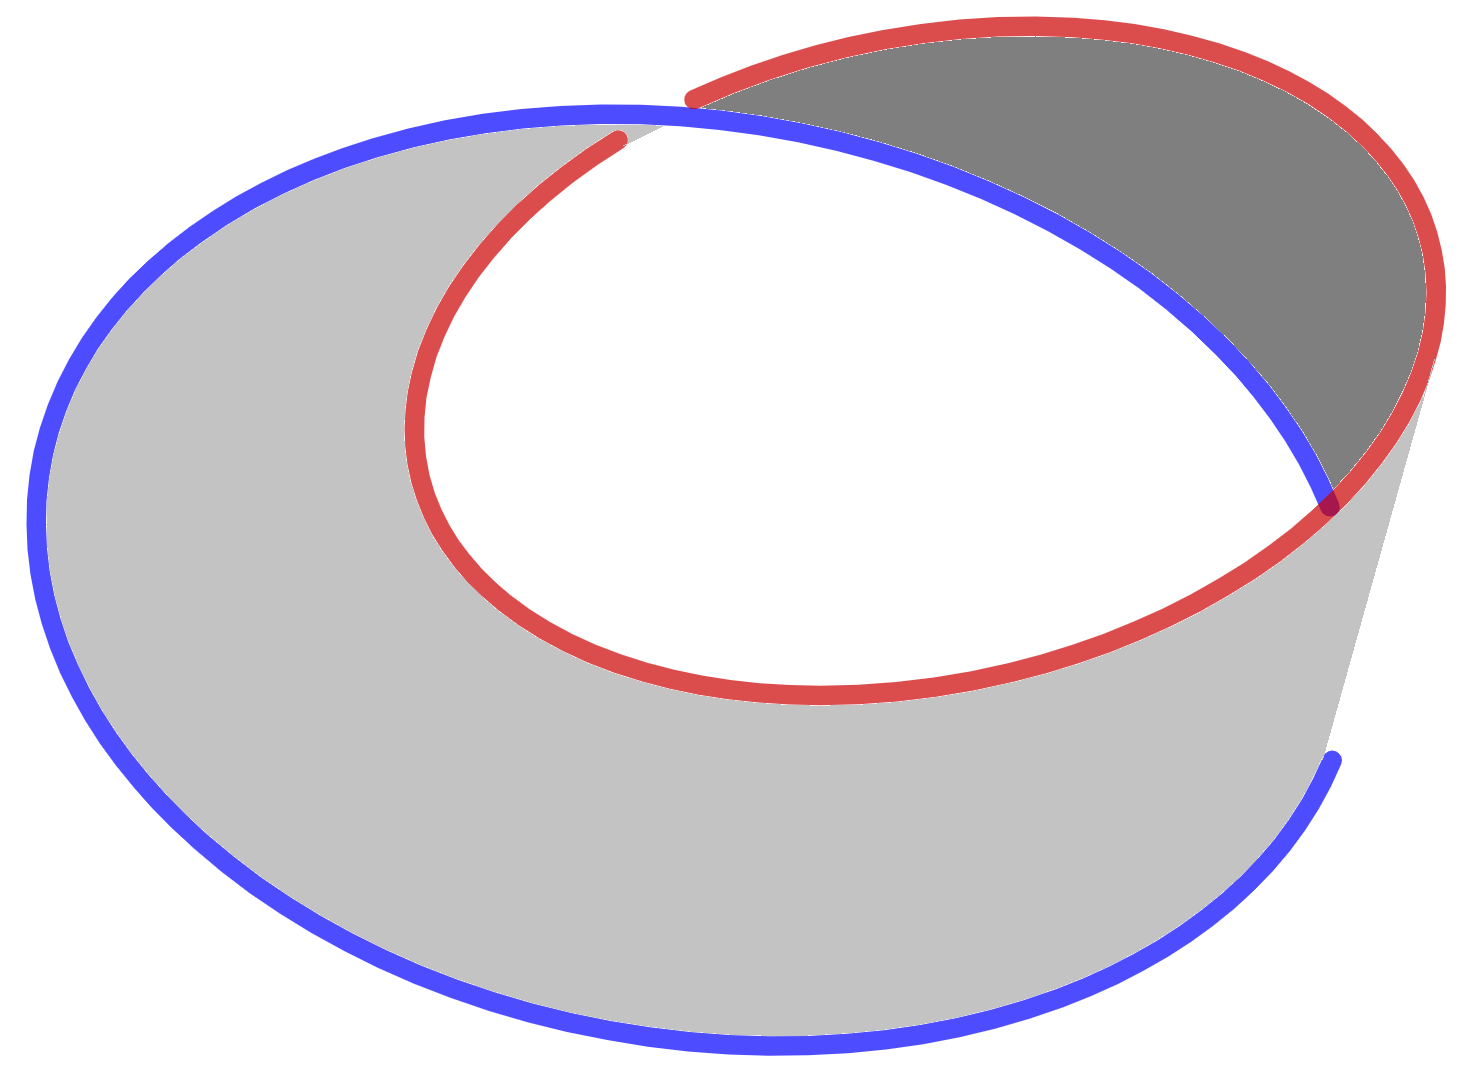
\includegraphics[width= 0.4\linewidth]{seifert2}
		\caption{\small\textit{\color{duongvaotoanhoc}Hình $12$: Mặt Seifert của nút ba lá và của liên kết Hopf (mặt M\"obius).}}
		\vspace*{-10pt}
	\end{figure}
	Sự tương tự tiếp theo: với $p$ là một số nguyên tố, ta xét vành $\mathbb{Z}_p$ các số nguyên $p$--adic cũng như trường $\mathbb{Q}_p$ các số $p$--adic. So với $\text{Spec}(\mathbb{Z})$, phổ $\text{Spec}(\mathbb{Z}_p)$ chỉ còn $2$ điểm là điểm tổng quát $\text{Spec}(\mathbb{Q}_p)$ và điểm đóng $\text{Spec}(\mathbb{F}_p)$, vì thế ta gọi thao tác này {\bf\color{duongvaotoanhoc} địa phương hóa} (tập trung nhìn vào số nguyên tố $p$ và quên đi các số nguyên tố khác). Thao tác này ứng với việc lấy {\bf\color{duongvaotoanhoc} lân cận ống} $V$ của nút, kết quả thu được là một hình xuyến đặc. Dù hình xuyến đặc không đồng phôi với đường tròn, chúng {\bf\color{duongvaotoanhoc} tương đương đồng luân với nhau}, điều này ứng với việc $\text{Spec}(\mathbb{Z}_p)$ và $\text{Spec}(\mathbb{F}_p)$ {\bf\color{duongvaotoanhoc} tương đương đồng luân étale với nhau}. Khi bỏ nút ban đầu khỏi $V$, ta thu được một không gian tương đương đồng luân với mặt xuyến (rỗng). Nhóm cơ bản của mặt xuyến là $\mathbb{Z} \times \mathbb{Z}$, một nhóm được sinh bởi hai phần tử là hai khuyên như trong Hình $13$.
	\begin{figure}[H]
		\vspace*{-5pt}
		\centering
		\captionsetup{labelformat= empty, justification=centering}
		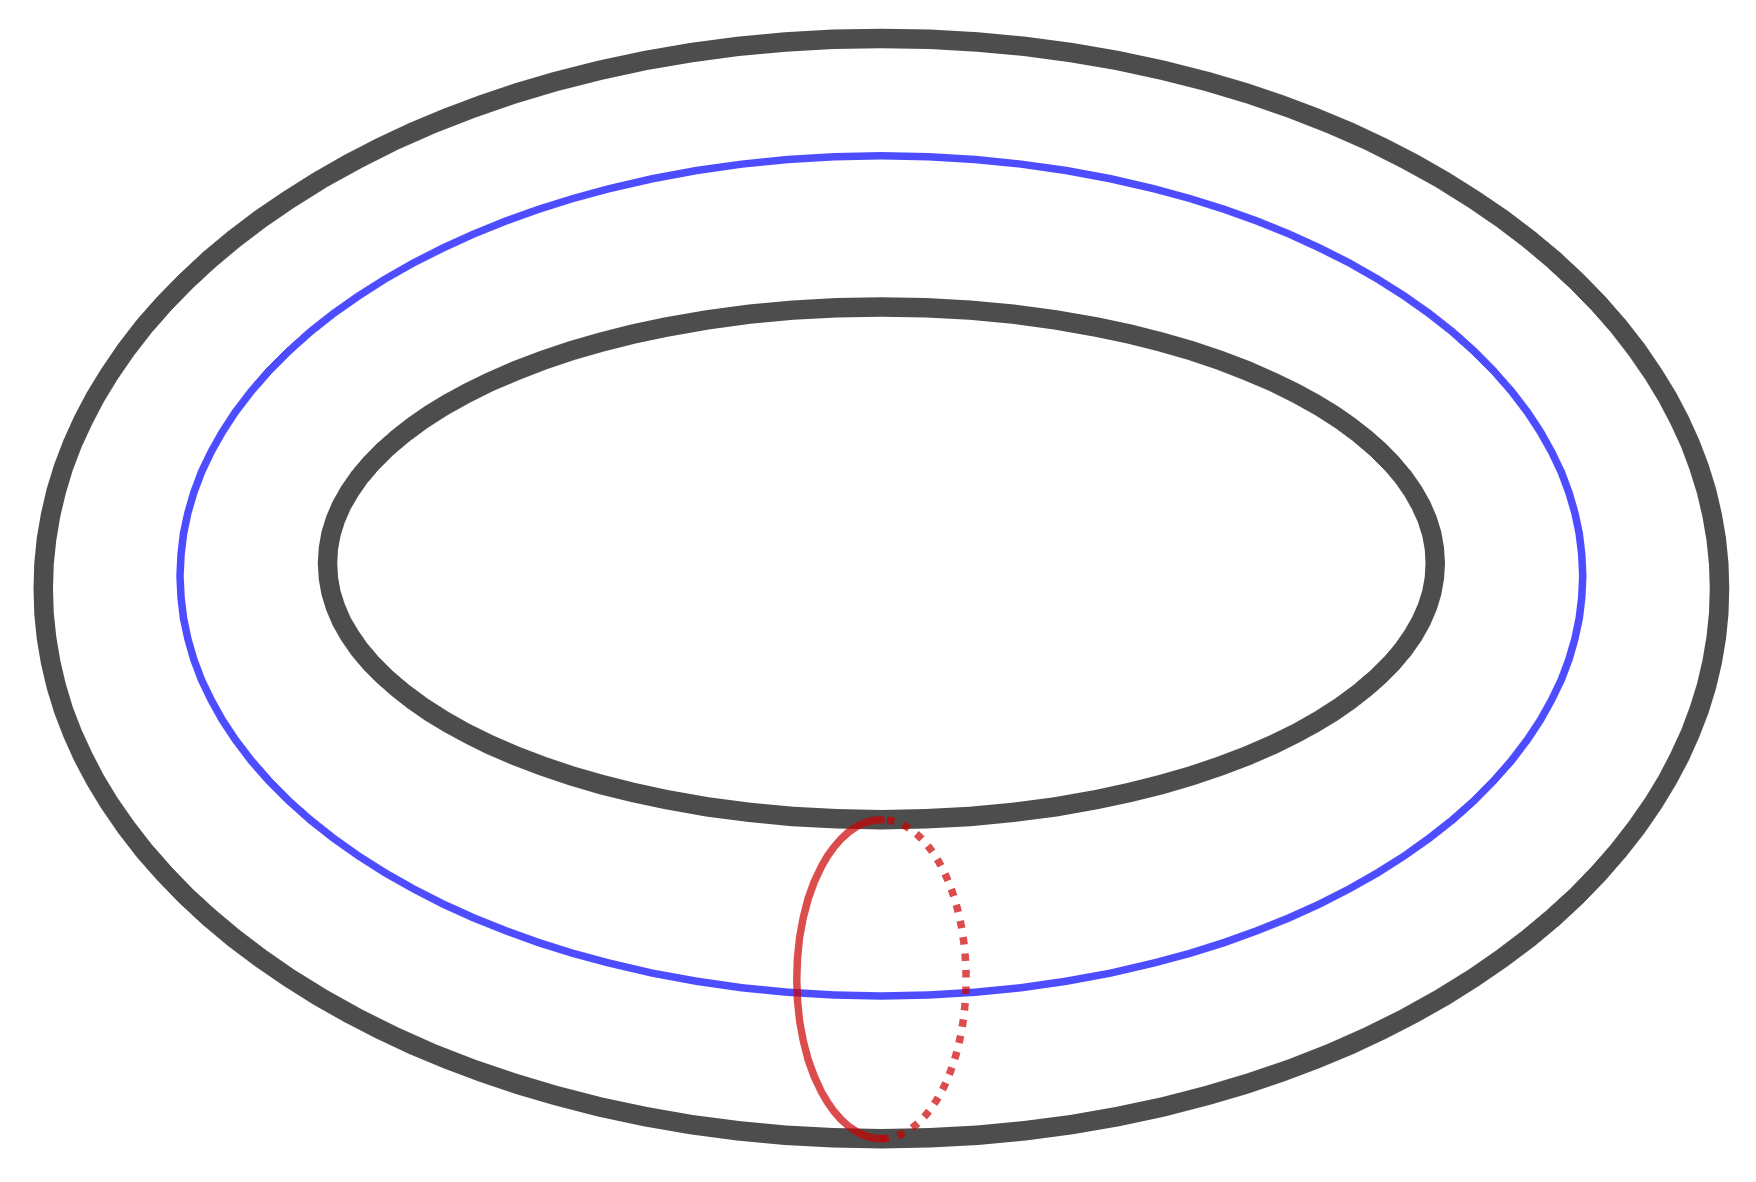
\includegraphics[width= 0.7\linewidth]{h13}
		\caption{\small\textit{\color{duongvaotoanhoc}Hình $13$: Nhóm cơ bản của mặt xuyến được sinh bởi hai khuyên màu xanh và màu đỏ.}}
		\vspace*{-10pt}
	\end{figure}
	Tương ứng, khi bỏ $\text{Spec}(\mathbb{F}_p)$ khỏi $\text{Spec}(\mathbb{Z}_p)$, ta thu được $\text{Spec}(\mathbb{Q}_p)$, và {\bf\color{duongvaotoanhoc} nhóm Galois rẽ nhánh yếu} (một phiên bản nhỏ hơn của nhóm cơ bản étale) của $\mathbb{Q}_p$ cũng được mô tả bởi $2$ phần tử sinh. Sau cùng, lý thuyết trường các lớp địa phương của Tate cho ta các đối ngẫu hoàn hảo giữa đối đồng điều Galois của  $\mathbb{Q}_p$ ở bậc $0$ và bậc $2$, cũng như ở bậc $1$ và chính nó. Tương ứng, ta có đối ngẫu Poincaré cho mặt xuyến, một đa tạp đóng $2$--chiều.
	\vskip 0.1cm
	\textbf{\color{duongvaotoanhoc}Thao tác trên biểu đồ phẳng}
	\vskip 0.1cm
	Quay lại với sự đẳng luân của các nút. Một câu hỏi rất tự nhiên là làm thế nào để chứng minh hai nút không đẳng luân? Đẳng luân vốn là một điều kiện tôpô quá khó sử dụng. Một khó khăn khi sử dụng các biểu đồ phẳng là hai nút đẳng luôn có thể cho hai biểu đồ phẳng trông rất khác nhau. Vậy vấn đề đầu tiên là ta cần tìm cách phân biệt hai nút qua biểu đồ phẳng của chúng (bài toán nhận biết nút). Điều này có thể được thực hiện một cách tổ hợp. Cụ thể, hai biểu đồ phẳng biểu diễn hai nút đẳng luân khi và chỉ khi tồn tại một chuỗi hữu hạn các thao tác thuộc một trong $4$ kiểu, được gọi là các {\bf\color{duongvaotoanhoc} chuyển động Reidemeister}.
	\begin{figure}[H]
		\vspace*{-5pt}
		\centering
		\captionsetup{labelformat= empty, justification=centering}
		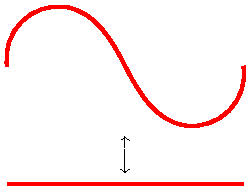
\includegraphics[width= 0.35\linewidth]{R0.pdf}\quad
		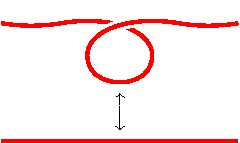
\includegraphics[width= 0.35\linewidth]{R1.pdf}
		\caption{\small\textit{\color{duongvaotoanhoc}R$0$: Phép đẳng luân phẳng.\hspace*{20pt}  RI: Phép xoắn.}}
		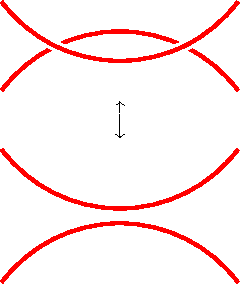
\includegraphics[width= 0.35\linewidth]{R2.pdf}\quad
		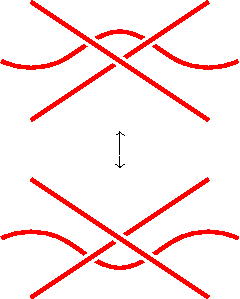
\includegraphics[width= 0.35\linewidth]{R3.pdf}
		\caption{\small\textit{\color{duongvaotoanhoc}RII: Phép đè.\hspace*{30pt} RIII: Phép trượt.}}
		\caption{\small\textit{\color{duongvaotoanhoc}Hình $14$: Các chuyển động Reidemeister.}}
		\vspace*{-10pt}
	\end{figure}
	Từ biểu đồ phẳng của nút, ta dùng các đại lượng không đổi qua các biến đổi Reidemeister, các {\bf\color{duongvaotoanhoc} bất biến nút}. Hai nút có bất biến khác nhau thì phải khác nhau. Một ví dụ như vậy là {\bf\color{duongvaotoanhoc} bất biến tô màu}. Ta nói một biểu đồ phẳng của nút là {\bf\color{duongvaotoanhoc} tô được bằng $3$ màu} nếu mỗi sợi (phần đường cong liên tục giữa hai giao điểm liên tiếp của nút) đều có thể tô được bằng một trong $3$ màu cho trước, sao cho
	\vskip 0.1cm
	$\bullet$ ít nhất hai màu phải được dùng;
	\vskip 0.1cm
	$\bullet$ tại mỗi giao điểm, sợi trên cùng $2$ sợi dưới hoặc là được tô cùng màu, hoặc là được tô $3$ màu khác nhau.
	\vskip 0.1cm
	Ví dụ, nút ba lá hiển nhiên tô được bằng $3$ màu, nút tầm thường hiển nhiên không tô được bằng $3$ màu. Nút số $8$ cũng không tô được bằng $3$ màu. Vậy ít nhất ta biết rằng nút $3$ lá không đẳng luân với nút tầm thường cũng như nút số $8$.
	\vskip 0.1cm
	Hiển nhiên là bất biến tô màu chỉ cho phép phân loại các nút thành $2$ lớp. Ta cần các loại bất biến khác. Ví dụ, xét nút ba lá trái và ảnh gương của nó là nút ba lá phải. Tất nhiên cả hai đều tô được bằng $3$ màu. Rất ngạc nhiên, hai nút này không đẳng luân! Hãy thử dùng các biến đổi Reidemeister để gỡ nút này thành nút kia và bạn sẽ sớm bị thuyết phục. Một bất biến cho phép phân biệt hai nút này là {\bf\color{duongvaotoanhoc} đa thức Alexander}. Đa thức này đến từ {\it lý thuyết Alexander--Fox}, và người ta phát hiện ra phiên bản số học của nó là {\it lý thuyết Iwasawa}. Sự song song của chúng cho phép ta dịch các kết quả từ một bên sang bên còn lại.
	\begin{figure}[H]
		\vspace*{-5pt}
		\centering
		\captionsetup{labelformat= empty, justification=centering}
		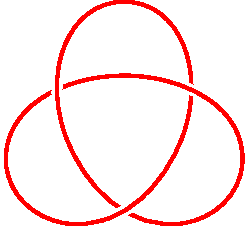
\includegraphics[width= 0.38\linewidth]{trefoil.pdf}\quad\quad
		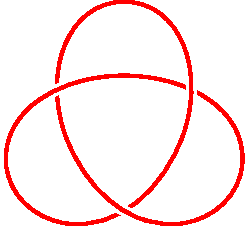
\includegraphics[width= 0.38\linewidth]{mirror trefoil.pdf}
		\caption{\small\textit{\color{duongvaotoanhoc}Hình $15$: Nút ba lá trái và nút ba lá phải.}}
		\vspace*{-10pt}
	\end{figure}
	Một kiểu bất biến khác cho liên kết là {\bf\color{duongvaotoanhoc} số liên kết}. Xét một liên kết được tạo bởi hai nút. Giữa hai nút $L$ và $K$, ta có thể định nghĩa {\bf\color{duongvaotoanhoc} số liên kết} qua biểu đồ phẳng của chúng như sau. Chẳng hạn, tô màu đỏ cho $L$ và màu xanh cho $K$, đồng thời định hướng cho chúng (mỗi nút có thể có $1$ trong $2$ hướng). Tại các điểm trên biểu đồ phẳng mà có một sợi của nút này nằm trên một sợi của nút kia hoặc ngược lại, ta đánh dấu $+$ hoặc $-$ theo quy tắc ở Hình $16$. Sau đó ta lấy số dấu cộng trừ đi số dấu trừ, và lấy kết quả chia đôi. Kết quả cuối cùng thu được được gọi là số liên kết $\text{lk}(L,K)$. Chẳng hạn, số liên kết của hai nút trong liên kết Hopf là $1$ hoặc $-1$, tùy theo cách định hướng hai nút.
	\begin{figure}[H]
		\vspace*{-5pt}
		\centering
		\captionsetup{labelformat= empty, justification=centering}
		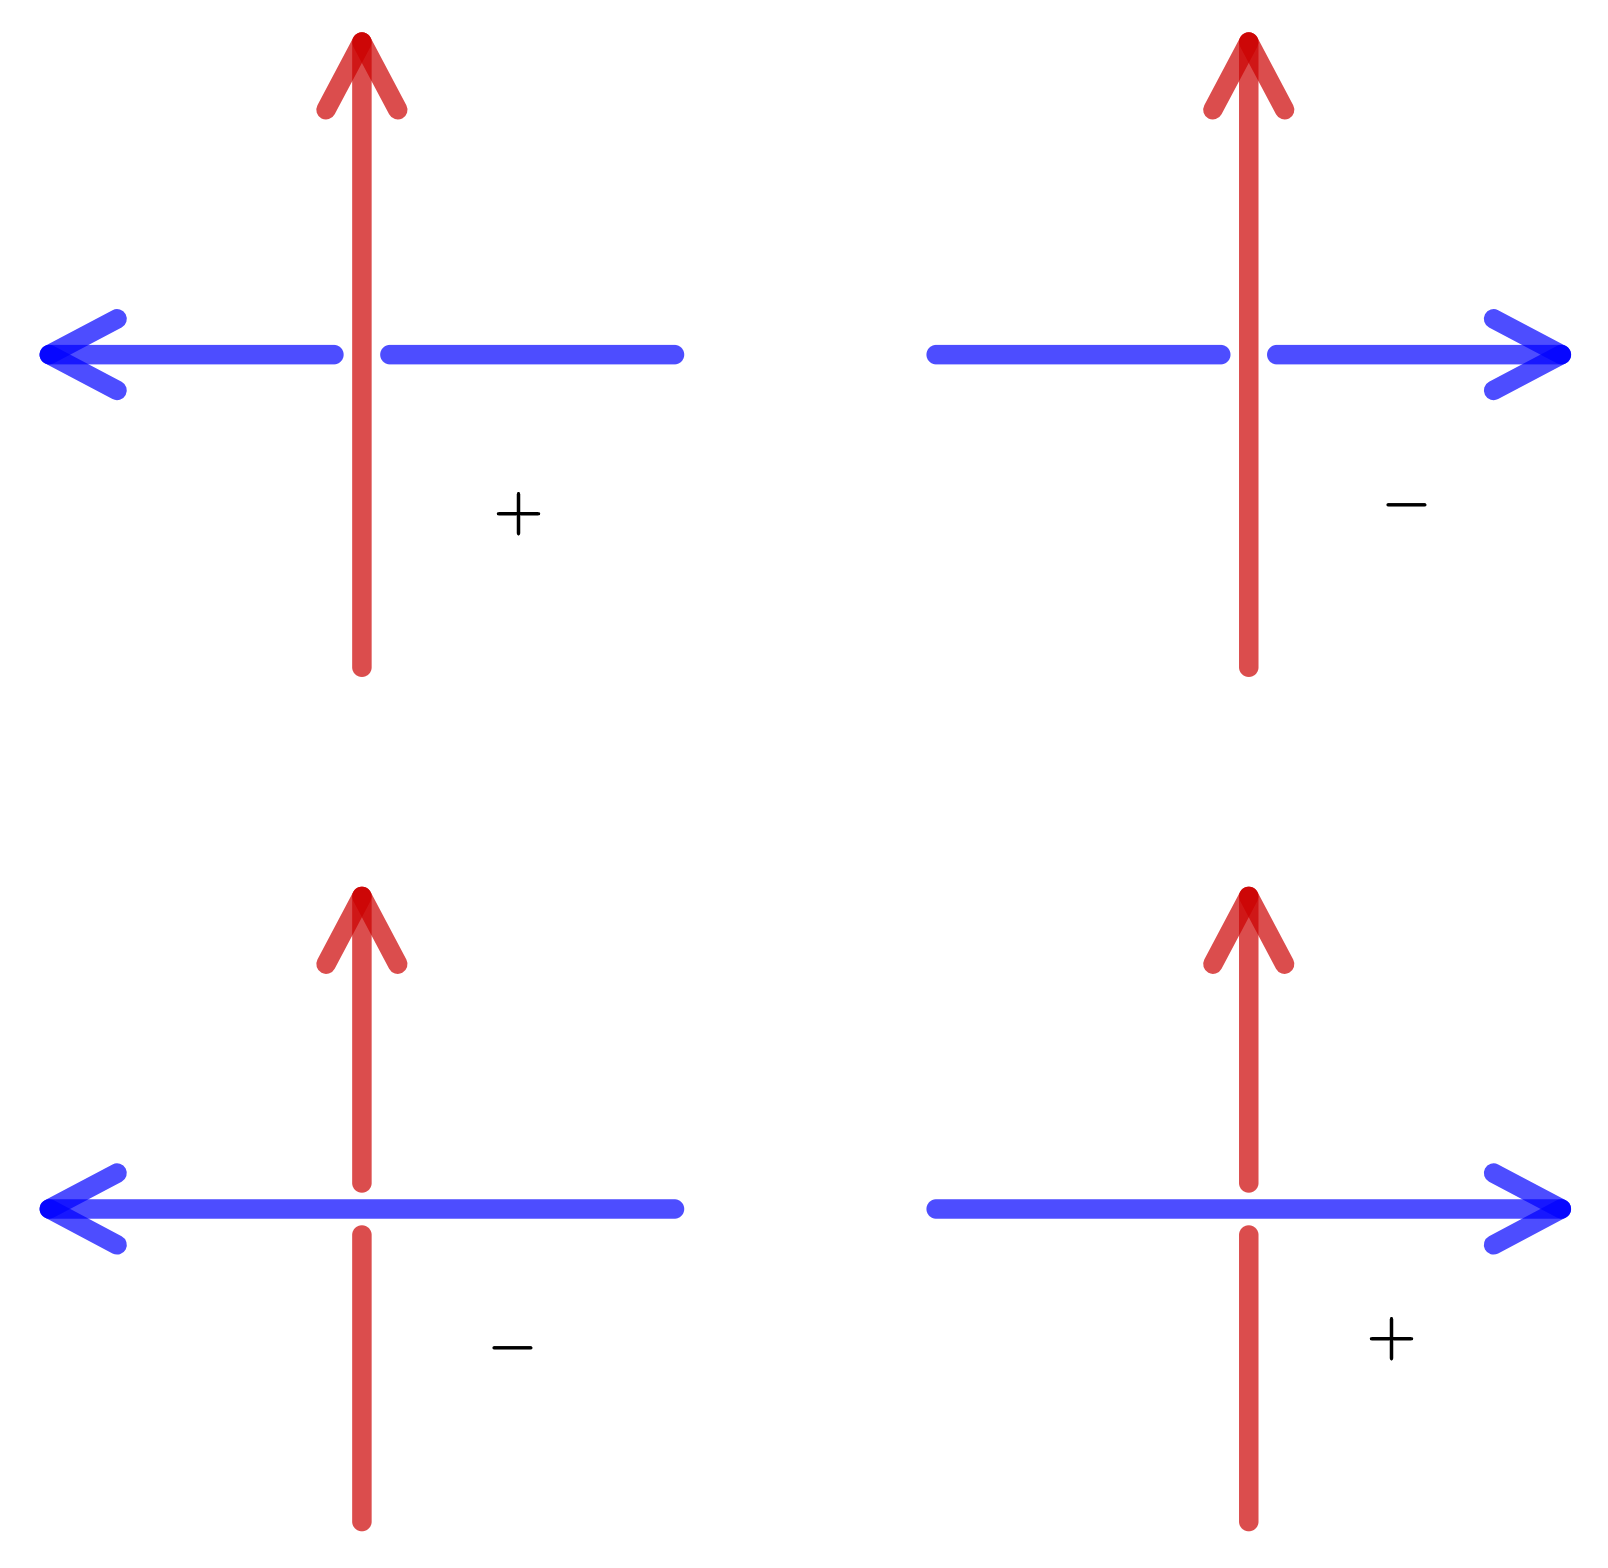
\includegraphics[width= 0.65\linewidth]{h16}
		\caption{\small\textit{\color{duongvaotoanhoc}Hình $16$: Quy tắc tính số liên kết.}}
		\vspace*{-10pt}
	\end{figure}
	Nhiều tính toán cho thấy rằng số liên kết thỏa mãn các tính chất tương tự như {\bf\color{duongvaotoanhoc} ký hiệu Legendre} $\left(\dfrac{p}{q}\right)$ giữa hai số nguyên tố $p, q$ trong lý thuyết thặng dư bậc hai. Ta có thể chứng minh rằng $\text{lk}(K,L) = \text{lk}(L,K)$. Tương ứng, ta có luật tương hỗ bậc hai, nói rằng 
	\begin{align*}
		\left(\dfrac{p}{q}\right) = (-1)^{\tfrac{(p-1)(q-1)}{4}}\left(\dfrac{q}{p}\right).
	\end{align*}
	Bài toán trung tâm của tôpô số học có lẽ là câu hỏi tự nhiên nhất: số nguyên tố nào ứng với nút nào? Đây vẫn là một câu hỏi mở. Nếu một ngày người ta xây dựng được một tương ứng $1-1$ tốt giữa chúng, theo nghĩa mỗi kết quả với số nguyên tố thì ta có kết quả với các nút tương ứng, một số lượng khổng lồ bài toán tôpô học sẽ được giải bằng các kết quả tương tự ở lý thuyết số, và ngược lại. Có thể nói, tôpô số học là một trong những ví dụ điển hình nhất về tư tưởng toán học thống nhất, rằng tất cả những đại số, giải tích, hình học, số học... đều chỉ là một.
\end{multicols} 
	\newpage

%	\setcounter{figure}{0}
%	\thispagestyle{quantoannone}
\pagestyle{quantoan}
\everymath{\color{quantoan}}
\graphicspath{{../quantoan/pic/}}
%\blfootnote{\color{quantoan}\color{quantoan}$^*$Nguồn Math. Intellegencer, Số $41$.}
\begingroup
\AddToShipoutPicture*{\put(0,616){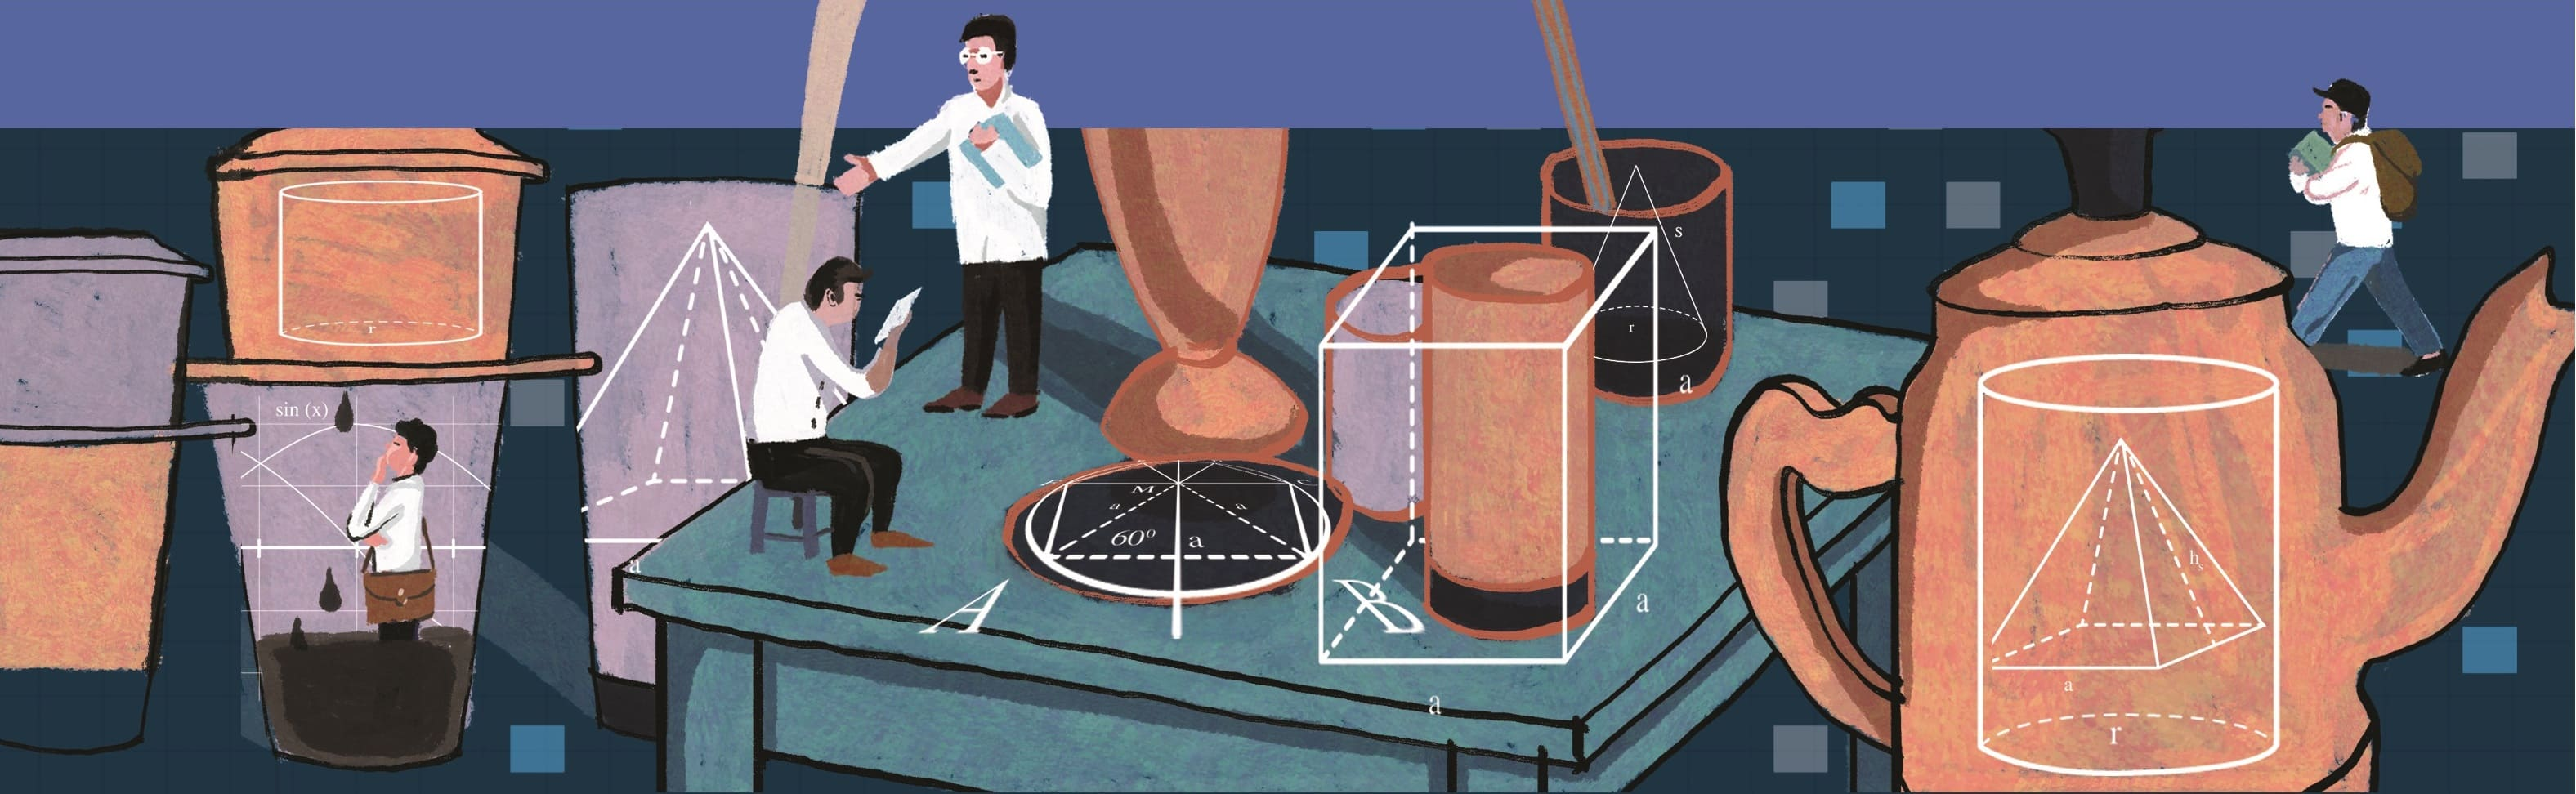
\includegraphics[width=19.3cm]{../bannerquantoan}}}
\AddToShipoutPicture*{\put(104,495){
\includegraphics[scale=1]{../tieude.pdf}}}
\centering
\endgroup

\vspace*{218pt}
\textit{\textbf{\color{quantoan}LTS.} Chuyên mục Danh ngôn Toán học giới thiệu với bạn đọc về lịch sử, ý nghĩa của những phát ngôn bởi các nhà toán học nổi tiếng. Ban biên tập Pi trân trọng mời bạn đọc đóng góp cho chuyên mục này.}

\vspace*{-5pt}
\begin{multicols}{2}
	Vào khoảng ba thế kỷ trước Công nguyên có một người Hy Lạp tên là Euclid từ xứ Alexandria. Họ gọi ông là như vậy, vì không ai biết họ của ông là gì. Ông lang thang ở thành Alexandria và trong thời gian rỗi, ông đã viết ra một bộ sách giáo khoa về hình học mà ông đặt tên là Cơ sở. Có lẽ ông đã được đào tạo sớm từ các học trò của Plato ở Athens, sau đó tiếp tục thành lập một trường học ở Alexandria vào năm $306$ trước Công nguyên. 
	\vskip 0.1cm
	Vào thời đó, có một nhà cai trị và tướng quân người Macedonia thuộc Hy lạp  là Ptolemy I Soter . Ông từng là vệ sỹ riêng của Alexander Đại đế, cũng đồng thời là một pharaoh của Ai Cập. Ptolemy I, giống như Alexander, rất quan tâm đến việc thúc đẩy nghiên cứu học thuật, và ông là người bảo trợ cho việc khai phá tri thức, sáng lập ra Đại Thư viện Alexandria. Ông ta tập hợp những ``người có học" xung quanh cung đình của mình.  Những người được biết đến là ``các bạn bè" này, bất kể là người đó là quý tộc hay thường dân, phục vụ Ptolemy với vai trò là các cố vấn chính của ông. Danh tiếng về bản tính nhân từ và phóng khoáng của tướng quân Ptolemy I đã gắn kết tầng lớp lính tráng trôi nổi nay đây mai đó, gồm cả những người Macedonia và những người Hy Lạp khác  tới phục vụ quanh ông. Chính Ptolemy đã viết cuốn Sử lược về các chiến dịch của Alexander, đã thất truyền. Đây từng được coi là một tác phẩm khách quan, nổi bật bởi tính trung thực và sự tỉnh táo trong nhận định. 
	\begin{figure}[H]
		\vspace*{-5pt}
		\centering
		\captionsetup{labelformat= empty, justification=centering}
		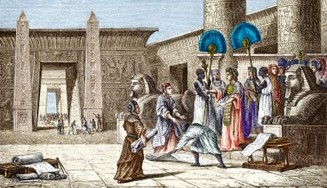
\includegraphics[width= 1\linewidth]{1}
		\caption{\small\textit{\color{quantoan}Hình $1$. Ptolemy I Soter ($366-282$ TCN), vị pharaoh Ai cập đồng thời là tướng quân người Macedonia thuộc Hy lạp.}}
		\vspace*{-12pt}
	\end{figure}
	Ptolemy I cũng  từng mời Triết gia nổi tiếng Strabo đến Alexandria làm gia sư cho con trai mình. Và khá đặc biệt, nhà toán học Euclid cũng là một trong những học giả được Prolemy bảo trợ. Tướng quân Ptolemy thấy tác phẩm tiêu biểu của Euclid, cuốn Cơ sở, quá khó để lĩnh hội, vì vậy ông ta  đã hỏi liệu có cách nào dễ dàng hơn để nắm vững được nó không. Và Euclide, theo ghi chép lại của Triết gia Proclus, đã có câu nói châm biếm nổi tiếng sau để trả lời Ptolemy ``Thưa Đức Ngài, không có con đường hoàng gia nào dẫn tới hình học".
	\begin{figure}[H]
		\vspace*{-5pt}
		\centering
		\captionsetup{labelformat= empty, justification=centering}
		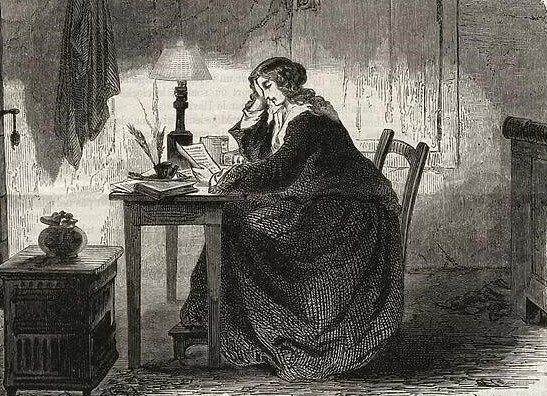
\includegraphics[width= 0.6\linewidth]{4}
		\caption{\small\textit{\color{quantoan}Hình $3$. Euclid, hay Kiến trúc. Tranh đá cẩm thạch, tầng hầm tháp chuông Florence, Ý.}}
		\vspace*{-10pt}
	\end{figure}
	Cụm từ ``con đường hoàng gia" thời đó chỉ  con đường đặc biệt được xây dựng xuyên qua Anatolia và Ba Tư bởi Darius Đại đế của Ba Tư (Darius I), cho phép liên lạc và chuyển quân nhanh chóng, nhưng Euclide đã sử dụng từ Hy lạp  ἀτραπός nghĩa là ``lối đi" (chứ không phải từ ὁδός ``con đường")  để truyền đạt ý nghĩa của ``đường tắt".
	\begin{figure}[H]
		\vspace*{-5pt}
		\centering
		\captionsetup{labelformat= empty, justification=centering}
		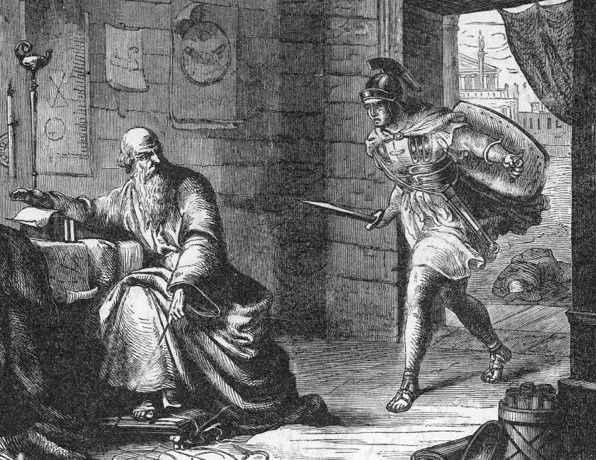
\includegraphics[width= 0.6\linewidth]{2}
		\caption{\small\textit{\color{quantoan}Hình $3$. Darius Đại đế của Ba Tư ($550-486$ TCN).}}
		\vspace*{-10pt}
	\end{figure}
	Tất nhiên, Eclide đã  nói bằng tiếng Hy Lạp với hy vọng Ptolemy sẽ hiểu ra rằng không có một điểm thưởng nào cho những ai chỉ đơn giản có mặt để điểm danh qua loa, khi muốn học môn hình học cho đến nơi đến chốn.
	\vskip 0.1cm
	Rất thú vị, ngày nay cụm từ ``con đường hoàng gia" đã vượt qua khuôn khổ của hình học và toán học, với ý nghĩa mới là ``con đường dẫn tới đích dễ dàng và nhanh nhất, không tốn công sức". Người ta có thể nói, ``đội bóng, sau khi đã loại tất cả các đối phương trong cùng nhóm, hiện đang trên con đường hoàng gia dẫn tới chức vô địch lần đầu tiên trong lịch sử thông qua đá loại trực tiếp", ``hãng phim nọ đang trên con đường hoàng gia đơn độc thống trị cả nền sản xuất điện ảnh và  tạo ra một thế độc quyền trong nền công nghiệp mà họ đang tích cực khai thác". Và tất nhiên, khi học tiếng Anh, các bạn cũng đều biết tới câu nói ``there is no royal road to learning". Học tiếng Anh, cũng như học hình học, đòi hỏi phải luyện tập kiên trì để đạt tới thành công trong việc diễn tả lưu loát những ý nghĩ riêng của bản thân mà không phải học thuộc lòng những cách nói mẫu, tuy đẹp nhưng khác lạ với cách diễn đạt của chính mình. 
	\begin{figure}[H]
		\vspace*{-5pt}
		\centering
		\captionsetup{labelformat= empty, justification=centering}
		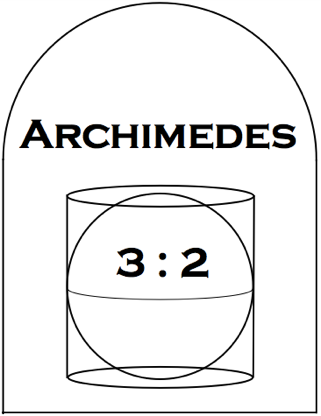
\includegraphics[width= 1\linewidth]{3}
		\caption{\small\textit{\color{quantoan}Hình $4$. Con đường hoàng gia của Ba Tư.}}
		\vspace*{-10pt}
	\end{figure}
	Còn trong môn hình học, cần rất nhiều kiên trì để hiểu và ghi nhớ những điều phức tạp của môn học, bao gồm các tính chất khác nhau của các hình khác nhau có hai chiều và ba chiều. Chỉ khi đó chúng ta mới có thể học được cách dựng và phân tích các hình hình học.
\end{multicols}
%	\newpage
%%	
%	\setcounter{figure}{0}
%	\thispagestyle{toancuabinone}
\pagestyle{toancuabi}
\everymath{\color{toancuabi}}
%\blfootnote{$^1$\color{toancuabi}Đại học Thăng Long.}
\graphicspath{{../toancuabi/pic/}}
\begingroup
\AddToShipoutPicture*{\put(0,616){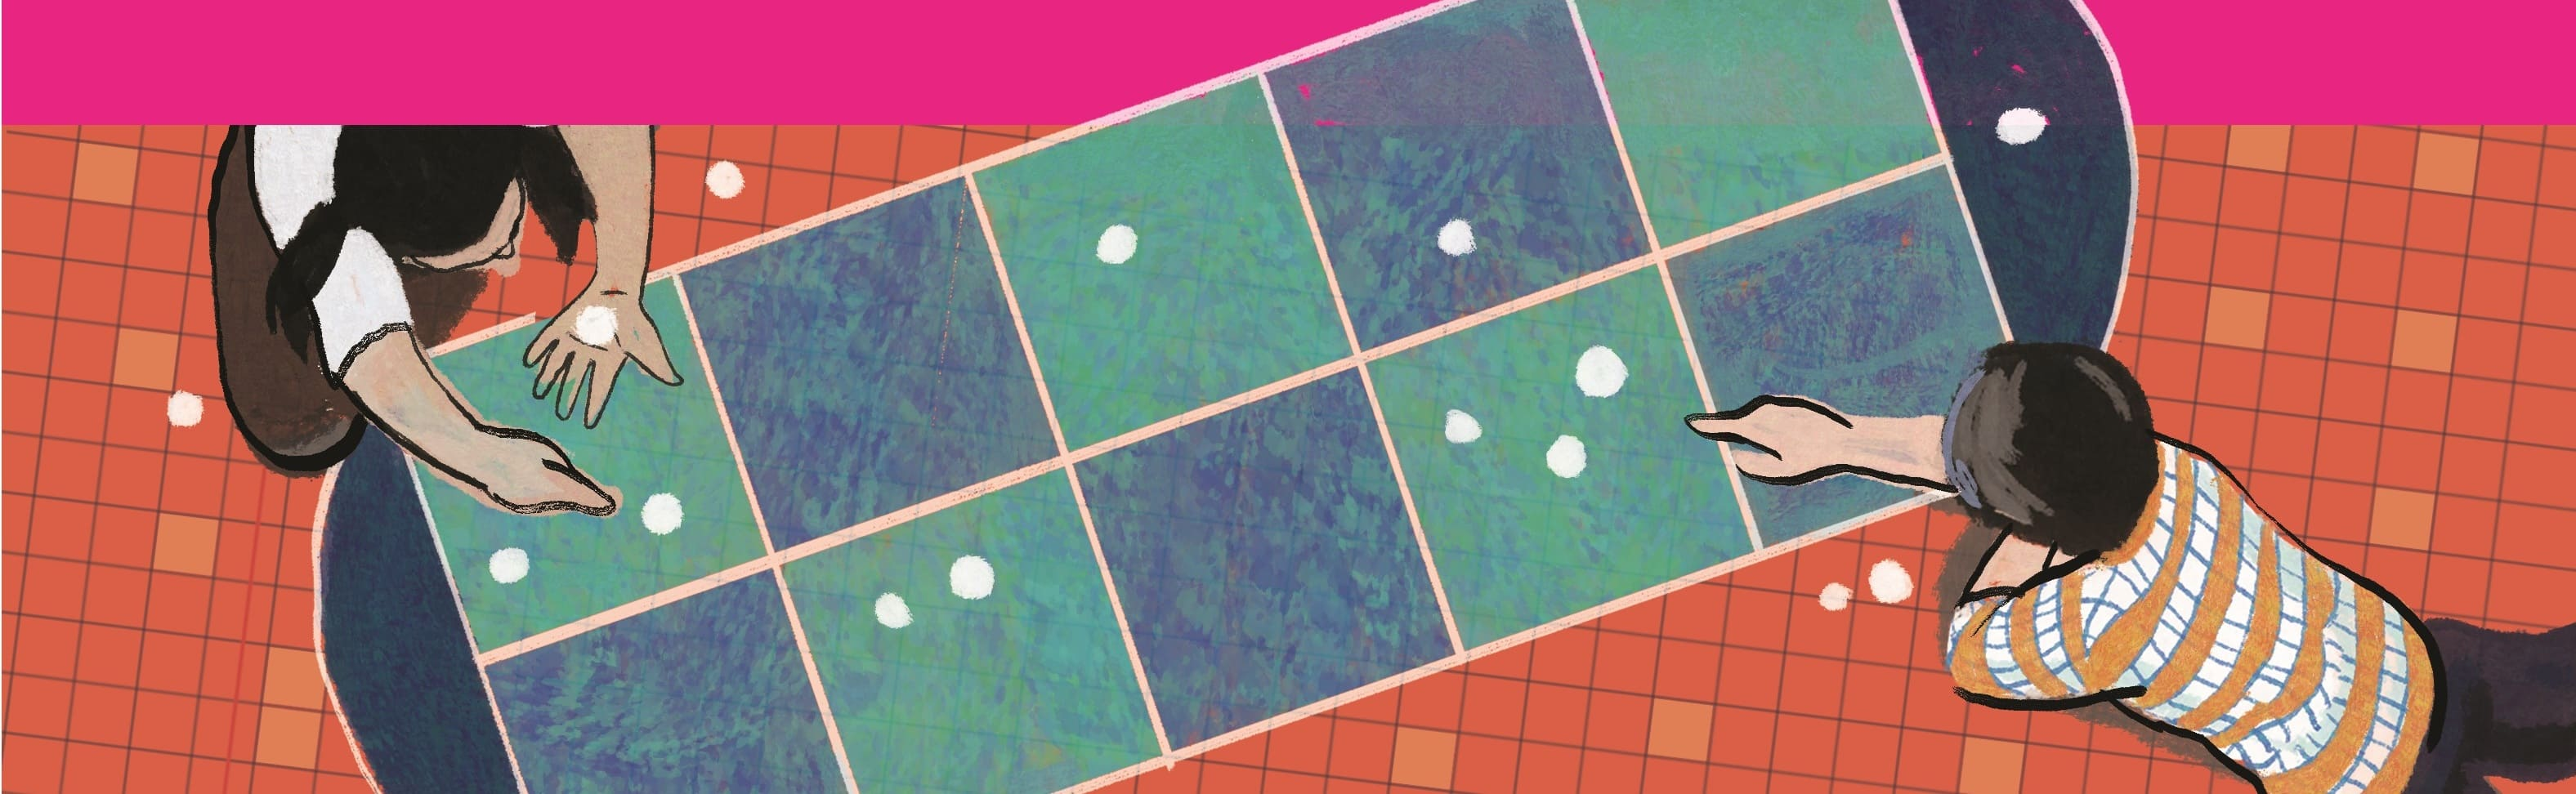
\includegraphics[width=19.3cm]{../bannertoancuabi}}}  
\AddToShipoutPicture*{\put(128,555){
\includegraphics[scale=1]{../tieude1.pdf}}} 
\centering
\endgroup
\vspace*{155pt} 

\begin{multicols}{2}
	Trò chơi ``Tháp Hà Nội", xếp những miếng gỗ trên ba chiếc cọc, đã rất quen thuộc với các bạn nhỏ Việt Nam cũng như nhiều bạn nhỏ trên thế giới. Thật là tuyệt vời khi một trò chơi nổi tiếng trên thế giới lại có tên liên quan đến thủ đô của nước ta đúng không. Các bạn đã biết về xuất xứ cùng với nhiều điều thú vị xung quanh bài toán ``Tháp Hà Nội" chưa? Chúng ta hãy cùng ngược dòng thời gian để tìm hiểu qua bài viết dưới đây nhé.
	\vskip 0.1cm
	Năm $1883$, Eduard Lucas (Claus) công bố  bức tranh quảng cáo ``Tháp Hà Nội --  trò chơi thực sự nát óc xứ Annnam":
	\begin{figure}[H]
		\centering
		\vspace*{-5pt}
		\captionsetup{labelformat= empty, justification=centering}
		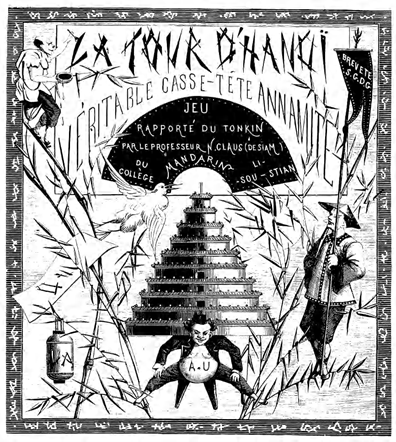
\includegraphics[width=1\linewidth]{1.1}
		%	\caption{\textit{\color{toancuabi}Hình $1$.}}
		\vspace*{-15pt}
	\end{figure}
	Một năm sau, Lucas viết bài ``Tháp Hà Nội , trò chơi toán học" đăng ở tạp chí ``Science et Nature", số $1$ ($1884$) tr. $127-128$. Có thể xem đó ngày khai sinh của ``Bài toán Tháp Hà Nội", một trong những bài toán nổi tiếng của toán học. Cho đến ngày nay, vẫn còn rất nhiều công trình nghiên cứu về bài toán tháp Hà Nội và những mở rộng của nó, vẫn còn nhiều giả thuyết đang chờ câu trả lời.
	\vskip 0.1cm
	Hình sau đây là bức ảnh chụp từ hiện vật trưng bày trong ``Musée des arts et métiers--Cnam Paris" (Bảo tàng nghệ thuật và thủ công Paris). 
	\begin{figure}[H]
		\centering
		\vspace*{-5pt}
		\captionsetup{labelformat= empty, justification=centering}
		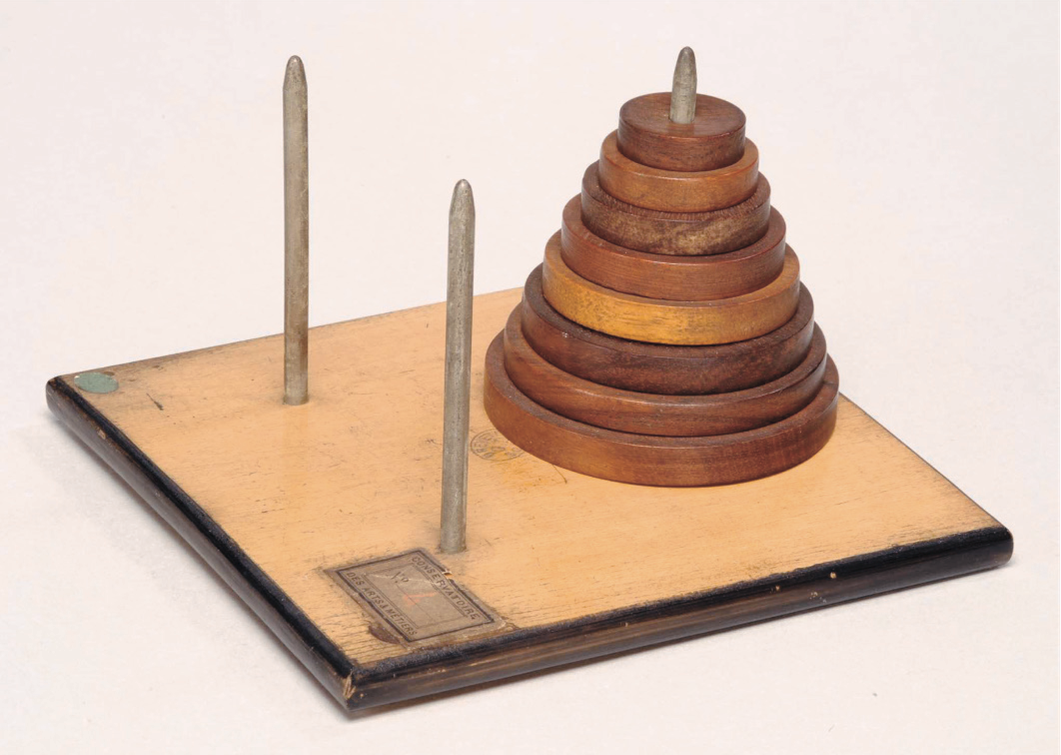
\includegraphics[width=1\linewidth]{2.1}
		%	\caption{\textit{\color{toancuabi}Hình $1$.}}
		\vspace*{-15pt} 
	\end{figure}
	Ta có ba cái cọc, và  $8$ cái đĩa với kích thước khác nhau đôi một. Bài toán đặt ra là di chuyển toàn bộ $8$ cái đĩa sang một cọc khác, sao cho vẫn giữ được thứ tự các đĩa với bán kính lớn dần từ trên xuống dưới. Quy tắc di chuyển: mỗi lần chỉ được chuyển một đĩa, và không bao giờ được đặt một đĩa lên đĩa khác có bán kính nhỏ hơn. Điều này có thể làm được nhờ sử dụng cọc ``trung gian".
	\vskip 0.1cm
	Các bạn thử hình dung xem ta sẽ cần làm bao nhiêu phép chuyển đĩa?
	\vskip 0.1cm
	Trước hết, ta thử làm bài toán dễ hơn: trên cọc chỉ có $2$ đĩa. Rõ ràng chỉ cần chuyển đĩa nhỏ sang cọc trung gian, đĩa lớn sang cọc còn lại, rồi chuyển đĩa nhỏ lên cọc đó. Số bước chuyển là $3$.
	\vskip 0.1cm
	Nếu có $3$ đĩa trên cọc thì sao? Giả sử các đĩa đang ở cọc $A$, và ta cần chuyển sang cọc $C$. Ta chuyển hai đĩa trên cùng sang cọc  trung gian $B$, rồi chuyển đĩa to nhất sang cọc $C$. Sau đó chỉ cần chuyển hai đĩa từ cọc $B$ sang cọc $C$. Phương pháp chuyển $2$ đĩa từ cọc này sang cọc khác thì ta đã biết. Như vậy, số phép chuyển phải làm khi có $3$ đĩa bằng $2$ lần số phép chuyên khi có $2$ đĩa, cộng thêm $1$ phép chuyển (đĩa to nhất). 
	\vskip 0.1cm
	Như vậy, số bước chuyển cần thiết của $3$ đĩa là: $2\times 3 + 1 = 7$. Bằng quy nạp, dễ chứng minh nếu $N$ là số phép chuyển khi có $n$ đĩa thì với $(n+1)$ đĩa, ta có thể thực hiện nhiệm vụ với $(2N+1)$ phép chuyển. Từ đó, dễ suy ra, nhiệm vụ đặt ra trong bài toán Tháp Hà Nội với $n$ đĩa có thể thực hiện với $2^n- 1$  phép chuyển.
	\vskip 0.1cm
	Có thể chứng minh $2^n - 1$  là số phép dịch chuyển tối thiểu cần thiết, nghĩa là không có cách gì thực hiện nhiệm vụ với số phép dịch chuyển ít hơn.
	\vskip 0.1cm
	Người ta cho rằng, bài toán Tháp Hà Nội lấy ý tưởng từ câu chuyển cổ Ấn Độ sau đây.
	\vskip 0.1cm
	``Trong ngôi đền vĩ đại ở Benares, bên dưới mái vòm đánh dấu trung tâm thế giới, người ta đặt một chiếc đĩa bằng đồng, trên đó gắn cố định ba chiếc cọc kim cương, mỗi chiếc cao một mét và dày như thân của một con ong. Trên một trong những chiếc cọc  kim cương đó, vào buổi sáng tạo, Thượng Đế đặt $64$ chiếc đĩa bằng vàng nguyên chất, theo thứ tự to dần từ trên xuống dưới.  Ngày đêm không ngừng, những con quỷ chuyển các đĩa từ cọc kim cương này sang cọc kim cương khác theo nguyên tắc không được di chuyển nhiều hơn một đĩa cùng một lúc, và không được đặt đĩa nào lên trên cái nhỏ hơn nó. Khi $64$ chiếc  đĩa  được chuyển xong thì tiếng sét sẽ nổ ra, và thế giới tan biến".
	\vskip 0.1cm
	Những suy luận trên đây chỉ ra rằng, số phép dịch chuyển mà lũ quỷ phải làm ít nhất là
	\begin{align*}
		2^{64} - 1= 18{.}446{.}744{.}073{.}709{.}551{.}615.
	\end{align*}
	Giả sử lũ quỷ rất thạo ``thuật toán dịch chuyển", và mỗi giây chúng chuyển được một đĩa, thì phải mất khoảng $585$ tỷ năm. Có lẽ dù không có lũ quỷ, trái đất của chúng ta cũng không tồn tại được lâu đến thế!
	\vskip 0.1cm
	Từ sau khi ra đời, bài toán Tháp Hà Nội nhận được sự quan tâm lớn của các nhà toán học và những người làm ... đồ chơi. Rất nhiều phiên bản của bài toán Tháp Hà Nội xuất hiện, chẳng hạn như số cọc lớn hơn $3$, hoặc cách chơi có thay đổi. Cho đến ngày nay, Tháp Hà Nội và những biến thể của nó vẫn là bài toán quan trọng trong toán học rời rạc, lý thuyết đồ thị, khoa học máy tính, và tô pô (chẳng hạn, bài toán về đường cong tự cắt tại mọi điểm của nó!). Thậm chí, Tháp Hà Nội còn có ứng dụng rộng rãi trong nghiên cứu tâm lý học!
	\vskip 0.1cm
	Người ta cho rằng, sở dĩ bài toán Tháp Hà Nội lôi cuốn được nhiều thế hệ các nhà toán học vì nó chứa đựng những yếu tố làm nên sức hấp dẫn của Toán học: đẹp, thú vị, hữu ích, và bất ngờ.
\end{multicols}
\newpage
\begingroup
\AddToShipoutPicture*{\put(56,678){\includegraphics[scale=0.95]{../tieude10.pdf}}} 
\centering
\endgroup
\vspace*{30pt}

\begin{multicols}{2}
	\textbf{\color{toancuabi}Ayatori} (hay trò chơi dây) là một trò chơi mà khi nhắc đến chắc chắn những người hâm mộ bộ truyện tranh Doraemon đều biết đến và nhớ ngay tới nhân vật Nobita. Trò chơi Ayatori là một trò chơi rất thú vị, người chơi sẽ sử dụng một sợi dây được buộc thành hình tròn, sau đó dùng những ngón tay của mình đan xen các sợi dây để tạo ra nhiều hình dạng khác nhau từ đơn giản đến phức tạp. Hôm nay, em hãy thử xếp hình ngôi sao thông qua trò chơi Ayatori nhé!
	\vskip 0.1cm
	\textit{Bước} $1$: Cách cầm dây khi mới bắt đầu chơi trò chơi Ayatori là giữ sợi dây trong ngón cái và ngón út bằng hai tay, rồi kéo ngang để chuẩn bị chơi.
	\begin{figure}[H]
		\vspace*{-10pt}
		\centering
		\captionsetup{labelformat= empty, justification=centering}
		\includegraphics[width=0.85\linewidth]{1a}
		
		\vspace*{1.8pt}
		\includegraphics[width=0.85\linewidth]{1b}
		
		\vspace*{1.5pt}
		\hspace*{3pt}\includegraphics[width=0.85\linewidth]{1c}
		\vspace*{-10pt}
	\end{figure}
	\textit{Bước} $2$: Thả dây ở hai ngón tay út. Sau đó dùng hai ngón tay út luồn phía dưới sợi dây ở hai ngón cái để kéo sợi dây ra như hình vẽ.
	\begin{figure}[H]
		\vspace*{-5pt}
		\centering
		\captionsetup{labelformat= empty, justification=centering}
		\includegraphics[width=0.85\linewidth]{2a}
%		\vspace*{-5pt}
	\end{figure}
	\begin{figure}[H]
		\vspace*{5pt}
		\centering
		\captionsetup{labelformat= empty, justification=centering}
		\includegraphics[width=0.85\linewidth]{2b}
		\vspace*{-5pt}
	\end{figure}
	\textit{Bước} $3$: Lấy ngón trỏ tay phải móc vào phần dây giữa ngón cái và ngón út của tay trái. Thực hiện tương tự với ngón trỏ tay trái.
	\begin{figure}[H]
		\vspace*{-5pt}
		\centering
		\captionsetup{labelformat= empty, justification=centering}
		\includegraphics[width=0.85\linewidth]{3a}
		
		\vspace*{1.8pt}
		\includegraphics[width=0.85\linewidth]{3b}
		
		\vspace*{2pt}
		\includegraphics[width=0.85\linewidth]{3c}
		
		\vspace*{1.8pt}
		\hspace*{2pt}\includegraphics[width=0.852\linewidth]{3d}
		\vspace*{-10pt}
	\end{figure}
	\textit{Bước} $4$: Thả dây ở hai ngón tay út.
	\begin{figure}[H]
		\vspace*{-5pt}
		\centering
		\captionsetup{labelformat= empty, justification=centering}
		\includegraphics[width= 0.85\linewidth]{4}
%		\caption{\small\textit{\color{}}}
		\vspace*{-10pt}
	\end{figure}
	\textit{Bước} $5$: Dùng ngón út để kéo sợi dây ở dưới cùng lên và chúng ta sẽ hoàn hành ngôi sao năm cánh.
	\begin{figure}[H]
		\vspace*{5pt}
		\centering
		\captionsetup{labelformat= empty, justification=centering}
		\includegraphics[width= 0.85\linewidth]{5}
%		\caption{\small\textit{\color{}}}
		\vspace*{-5pt}
	\end{figure}
	Hãy thử suy ngẫm xem hình ngôi sao năm cánh em vừa tạo ra có bao nhiêu trục đối xứng?
	\vskip 0.1cm
	\textbf{\color{toancuabi}Làm cây thông Noel}
	\vskip 0.1cm
	\textit{Bước} $1$: Xếp hai tờ giấy màu cứng chồng lên nhau rồi gấp đôi lại cho đều nhau. Sau đó lấy bút vẽ phác họa hình cây thông lên mặt ngoài của tờ giấy rồi dùng kéo cắt theo các đường đã vẽ sẵn. Lúc mở ra, em sẽ có hai cây thông với kích thước giống nhau.
	\begin{figure}[H]
		\vspace*{-5pt}
		\centering
		\captionsetup{labelformat= empty, justification=centering}
		\includegraphics[width= 1\linewidth]{6}
%		\caption{\small\textit{\color{}}}
		\vspace*{-15pt}
	\end{figure}
	\textit{Bước} $2$: Gấp đôi cây thông theo chiều ngang, gấp đầu nhọn xuống dưới để xác định tâm của mỗi cây thông. Tiếp đến dùng kéo cắt một đường từ đỉnh cây thông xuống điểm vừa đánh dấu. Cây thông còn lại thì cắt từ đáy lên điểm vừa đánh dấu.
	\begin{figure}[H]
		\vspace*{-5pt}
		\centering
		\captionsetup{labelformat= empty, justification=centering}
		\includegraphics[width= 1\linewidth]{7}
%		\caption{\small\textit{\color{}}}
		\vspace*{-15pt}
	\end{figure}
	\textit{Bước} $3$: Sau khi đã hoàn thành việc cắt hai cây thông, em hãy ghép chúng lại với nhau theo các khe đã cắt, chú ý để các góc không bị cong. Nếu sau khi ráp cây thông bị lung lay các em có thể cố định lại bằng keo dán.
	\begin{figure}[H]
		\vspace*{-5pt}
		\centering
		\captionsetup{labelformat= empty, justification=centering}
		\includegraphics[width= 1\linewidth]{8}
%		\caption{\small\textit{\color{}}}
		\vspace*{-15pt}
	\end{figure}
	\textit{Bước} $4$: Cuối cùng các em chỉ cần điều chỉnh sao cho cây thông đứng vững, trang trí thêm các dây ruy băng hay rắc kim tuyến,… hoặc vẽ họa tiết lên cây thông Noel để nhìn đẹp hơn.
	\begin{figure}[H]
		\vspace*{-5pt}
		\centering
		\captionsetup{labelformat= empty, justification=centering}
		\includegraphics[height= 0.31\linewidth]{9a}
		\includegraphics[height= 0.31\linewidth]{9b}
		\includegraphics[height= 0.31\linewidth]{9c}
		\caption{\small\textit{\color{toancuabi}Ảnh: Internet.}}
		\vspace*{-10pt}
	\end{figure}
	\textbf{\color{toancuabi}Bài tập}
	\vskip 0.1cm
	Còn gì tuyệt vời hơn khi được thả diều dưới bầu trời xanh và trong làn gió mát của những buổi chiều mùa hè oi ả. Bằng những kiến thức của bài ``Hình có trục đối xứng" và trí tưởng tượng phong phú của mình, em hãy tự làm ra cho mình một con diều đẹp đẽ với màu sắc rực rỡ nhé. Chúc em thành công!
	\begin{figure}[H]
		\vspace*{-5pt}
		\centering
		\captionsetup{labelformat= empty, justification=centering}
		\includegraphics[width= 1\linewidth]{10}
		\caption{\small\textit{\color{toancuabi}Hình ảnh con diều (Ảnh: Internet)}}
		\vspace*{-10pt}
	\end{figure}
\end{multicols}

\newpage
\begingroup
\AddToShipoutPicture*{\put(78,675){\includegraphics[scale=1]{../tieude.pdf}}} 
\centering
\endgroup
\vspace*{30pt}

\begin{multicols}{2}
	Thám tử Xuân Phong cùng thanh tra Lê Kính tham gia một buổi giới thiệu sản phẩm của hai công ty là Tae Yeon và TeaYon tại triển lãm Điện tử Expo -- New Vision của khu vực. Công ty  Tae Yeon có uy tín từ lâu đời, với những sản phẩm tinh tế có chất lượng tốt nổi tiếng,  các nhân viên của công ty luôn nói thật. Còn công ty TeaYon chuyên sản xuất đồ rẻ, kém chất lượng, bắt chước kiểu dáng của công ty Tae Yeon nên ban giám đốc dặn các nhân viên của mình chỉ được nói dối trong buổi triển lãm. 
	\vskip 0.1cm
	Vừa đặt chân tới khu vực triển lãm được trang hoàng lộng lẫy, Xuân Phong gặp ngay $5$ đại diện  của hai công ty này đứng tại cổng ra vào và tươi cười niềm nở tiếp đón. Xuân Phong tiến tới họ và hỏi cả $5$ người cùng một câu hỏi ``Có bao nhiêu người đến từ công ty Tae Yeon trong số các bạn?" 
	\vskip 0.1cm
	Người thứ nhất trả lời ``Không có ai cả". Hai người tiếp theo đều trả lời ``Có đúng một người". 
	\vskip 0.1cm
	Vậy hai người còn lại sẽ trả lời câu hỏi của thám tử Xuân Phong như thế nào nhỉ? Em có thể suy đoán ra câu trả lời của họ và giải thích lập luận được không?
	\begin{figure}[H]
		\centering
		\vspace*{-5pt}
		\captionsetup{labelformat= empty, justification=centering}
		\includegraphics[width=1\linewidth]{xuanphong}
		\vspace*{-5pt}
	\end{figure}
	%	
	%	Người của công ty Tae Yeon không thể trả lời ``Không có ai cả" vì như vậy người đó sẽ nói dối. Vì vậy, người đầu tiên đến từ công ty TeaYon. 
	%	\vskip 0.1cm
	%	Hai người tiếp theo trả lời giống nhau, vì thế họ phải cùng nói thật hoặc cùng nói dối, tức là đến từ cùng một công ty.
	%	\vskip 0.1cm
	%	Nếu cả hai người này cùng đến từ công ty Tae Yeon, suy ra số người của công ty Tae Yeon trong số họ không ít hơn $2$ người. Suy ra câu trả lời của họ là sai. Vì vậy cả hai người thứ hai và thứ ba đều nói dối, tức là đến từ công ty TeaYon.
	%	\vskip 0.1cm
	%	Do vậy, trong số $5$ người này, có ít nhất $3$ người của công ty TeaYon và không quá $2$ người đến từ công ty Tae Yeon.
	%	\vskip 0.1cm
	%	Nhưng vì cả $3$ người đầu tiên đều nói dối, suy ra số người của công ty Tae Yeon trong số họ không thể là $0$ hoặc $1$. Vì vậy, cả hai người còn lại đều là nhân viên của công ty Tae Yeon. Và họ đều sẽ trả lời là ``Có hai người".
\end{multicols}
\vspace*{-10pt}
{\color{toancuabi}\rule{1\linewidth}{0.1pt}}
\begingroup
\AddToShipoutPicture*{\put(115,305){\includegraphics[scale=1]{../tieude11.pdf}}} 
\centering
\endgroup
\vspace*{53pt}

\begin{multicols}{2}
	$\pmb{1.}$	Trong một cuộc thi thể thao, ban tổ chức chọn ra một số bạn học sinh ở lớp $5A$ và một số bạn ở lớp $5B$ thi đấu trực tiếp. Mỗi bạn ở lớp $5A$ được chọn ra sẽ thi đấu duy nhất một trận với một bạn ở lớp $5B$, và ngược lại, mỗi bạn ở lớp $5B$ được chọn ra chỉ đấu đúng một trận với một bạn ở lớp $5A$.
	\begin{figure}[H]
		\centering
		\vspace*{-5pt}
		\captionsetup{labelformat= empty, justification=centering}
		\includegraphics[width=1\linewidth]{Pi5_bai1}
		\vspace*{-15pt}
	\end{figure}
	Biết rằng số học sinh lớp $5A$ được chọn thi đấu chiếm $2/3$ tổng số học sinh toàn lớp $5A$, còn số học sinh lớp $5B$ được chọn thi đấu chiếm $3/5$ tổng số học sinh toàn lớp $5B$. Tổng số học sinh của cả hai lớp là $57$ bạn. Hỏi có bao nhiêu học sinh của hai lớp đã tham gia các trận thi đấu trực tiếp?
	
	$\pmb{2.}$ Công ty vận tải được thông báo ngắn gọn là có một số kiện hàng có tổng trọng lượng là $10$ tấn cần được vận chuyển, hơn nữa mỗi kiện hàng nặng không quá $1$ tấn. Hỏi công ty  cần điều động ít nhất bao nhiêu xe tải có trọng tải là $3$ tấn mỗi xe để luôn chắc chắn chở được hết được số hàng hoá đó?
	\begin{figure}[H]
		\centering
		%			\vspace*{-1pt}
		\captionsetup{labelformat= empty, justification=centering}
		\includegraphics[width=1\linewidth]{Pi5_bai2}
		\vspace*{-15pt}
	\end{figure}
	$\pmb{3.}$ Sau khi được sạc đầy pin, điện thoại di động của bạn An dùng đúng $6$ tiếng ở chế độ trò chuyện hoặc đúng $210$ tiếng ở chế độ chờ. Khi bạn An lên tàu hoả để đi du lịch, pin của bạn được sạc đầy $100\%$, và trên tàu không có ổ cắm sạc nên khi xuống ga, pin của bạn cũng vừa hết sạch. Biết rằng An đã nói chuyện với bạn bè đúng một nửa thời gian khi ngồi trên tàu, còn nửa thời gian còn lại đặt điện thoại ở chế độ chờ. Hỏi thời gian An đi trên tàu hoả là bao nhiêu lâu?
	\begin{figure}[H]
		\centering
		\vspace*{-5pt}
		\captionsetup{labelformat= empty, justification=centering}
		\includegraphics[width=1\linewidth]{Pi5_bai3}
		\vspace*{-15pt}
	\end{figure}
	$\pmb{4.}$ Một nhóm học sinh đi bộ từ điểm hẹn tới bến xe buýt để kịp đón chuyến xe vào lúc $8$ giờ. Cũng vào thời điểm này, từ điểm thăm quan, một chiếc xe buýt cũng xuất phát để tới kịp bến xe đón nhóm học sinh đó. Tuy  nhiên nhóm học sinh tới bến xe buýt khá sớm, vào lúc $6$ giờ $10$ phút, nên họ quyết định đi bộ tiếp tới điểm thăm quan. Trên đường, các bạn đã gặp được xe buýt và lên xe đi tiếp.  Cuối cùng cả nhóm đến được điểm thăm quan sớm hơn $20$ phút so với thời gian ấn định. Biết rằng vận tốc của xe buýt là $60$ km/h và vận tốc đi bộ của các em học sinh luôn không đổi. Hãy tìm vận tốc đi bộ của nhóm học sinh trước khi gặp xe buýt.
	\begin{figure}[H]
		\centering
		%			\vspace*{-5pt}
		\captionsetup{labelformat= empty, justification=centering}
		\includegraphics[width=1\linewidth]{Pi5_bai4}
		\vspace*{-10pt}
	\end{figure}
	$\pmb{5.}$ 	Có $100$ chiếc xe ô tô đỗ liền nhau thành một hàng dọc bên lề đường, trong đó có $70$ chiếc xe hiệu Mercedes, còn lại là những xe nhãn hiệu khác. Trong các xe nhãn hiệu Mercedes có $30$ chiếc màu đỏ, $20$ chiếc màu vàng và $20$ chiếc màu hồng. Biết rằng không có hai xe Mercedes nào khác màu lại đỗ cạnh nhau. Em hãy chỉ ra rằng luôn tìm ra $3$ chiếc xe Mercedes cùng màu đỗ liên tiếp nhau.
	\begin{figure}[H]
		\centering
		\vspace*{-5pt}
		\captionsetup{labelformat= empty, justification=centering}
		\includegraphics[width=1\linewidth]{Pi5_bai5}
		\vspace*{-15pt}
	\end{figure}
	$\pmb{6.}$ Một lớp học có $20$ em học sinh. Cô giáo chủ nhiệm của lớp tổ chức một số buổi thăm quan vào mỗi ngày cuối tuần trong suốt năm học, mỗi buổi tham quan có ít nhất $4$ em học sinh tham gia. Em hãy chứng minh rằng có một buổi thăm quan mà mỗi em học sinh tham gia buổi đó đều tham gia ít nhất $1/17$ tổng số tất cả các buổi tham quan của cả năm học.
	\begin{figure}[H]
		\centering
		\vspace*{-5pt}
		\captionsetup{labelformat= empty, justification=centering}
		\includegraphics[width=1\linewidth]{Pi5_bai6}
		\vspace*{-15pt}
	\end{figure}
\end{multicols}
\newpage
\begingroup
\AddToShipoutPicture*{\put(110,645){\includegraphics[scale=1]{../tieude2.pdf}}} 
\centering
\endgroup
\vspace*{55pt}

\begin{multicols}{2}
	$\pmb{1.}$ Một bác nông dân chở một xe ô tô quất cảnh ra chợ Tết để bán. Sau khi bán hết cây quất cuối cùng với giá $230$ nghìn đồng, bác tính nhẩm lại thấy mình đã bán số cây quất với giá trung bì nh là $245$ nghìn đồng/cây. Nhưng ngay lúc ấy người mua cây quất cuối quay trở lại và chỉ cho bác thấy cành quất bị rụng quá nhiều lá, nên ông ta chỉ đồng ý mua với giá $158$ nghìn đồng. 
	Bác chấp thuận và bán cây quất đó. Khi nhẩm tính lại, bác nông dân thấy giá trung bình của xe quất bây giờ là $242$ nghìn đồng. Hỏi bác đã bán được bao nhiêu cây quất?
	\begin{figure}[H]
		\centering
		\vspace*{-10pt}
		\captionsetup{labelformat= empty, justification=centering}
		\includegraphics[width=0.7\linewidth]{Pi1_2_Bai1}
		\vspace*{-15pt}
	\end{figure}
	\textit{Lời giải.} Gọi số cây quất là $n$, còn giá tiền một cây quất là $Q$ (nghìn đồng). Khi đó $Q+230 = 245n$ và $Q+ 158 = 242n$. Trừ hai đẳng thức này ta có $72 = 3n$. Suy ra bác nông dân đã bán được $24$ cây quất.
	\vskip 0.1cm
	$\pmb{2.}$ Chuyện kể rằng có một người khi gặp nhà triết học và toán học Hy--Lạp Pythagoras đã hỏi ông: ``Bây giờ là mấy giờ?" Pythagoras đã trả lời ``Cho đến hết ngày, còn lại hai lần của hai phần năm khoảng thời gian đã trôi qua từ lúc bắt đầu ngày". Nghe vậy, người đó chịu không thể nghĩ ra ngay được lúc họ gặp nhau là mấy giờ. Em có thể giúp trả lời lúc đó là mấy giờ được không?
	\vskip 0.1cm
	\textit{Lời giải.} 	Gọi $x$ là thời gian (tính theo giờ) đã trôi qua từ lúc bắt đầu ngày. Khi đó ta có hệ thức sau theo câu trả lời của Pythagoras: $24 - x = 4/5 x$. Suy ra $x = 40/3$ (giờ), có nghĩa là $13$ giờ $20$ phút. Vậy người đó đã gặp Pythagoras lúc $13$ giờ $20$ phút.
	\begin{figure}[H]
		\centering
		\vspace*{-10pt}
		\captionsetup{labelformat= empty, justification=centering}
		\includegraphics[width=0.6\linewidth]{Pi1_2_Bai2}
		\vspace*{-10pt}
	\end{figure}
	$\pmb{3.}$ Một tháng trước bà Hoa ra chợ mua một cân khoai tây, một cân thịt và một chục trứng. Chủ nhật vừa rồi, khoai tây tăng lên gấp $3$, thịt gấp $4$ lần còn trứng đắt gấp $5$ lần, nên bà Hoa phải trả $600$ nghìn cho từng ấy món hàng như lần thứ nhất. Hôm nay thì khoai lại đắt gấp $6$ lần so với tháng trước, thịt đắt gấp $5$ lần còn trứng chỉ đắt gấp $4$ lần nên bà Hoa lại phải trả $660$ nghìn với cùng một lượng hàng. Hỏi bà Hoa đã trả bao nhiêu tiền cho lần mua thứ nhất?
	\begin{figure}[H]
		\centering
		\vspace*{-10pt}
		\captionsetup{labelformat= empty, justification=centering}
		\includegraphics[width=0.7\linewidth]{Pi1_2_Bai3}
		\vspace*{-10pt}
	\end{figure}
	\textit{Lời giải.} 	Giả sử vào tháng trước trong lần mua đầu tiên giá một cân khoai tây là $a$ (nghìn đồng), giá một cân thịt là $b$ (nghìn đồng) và giá một chục trứng là $c$ (nghìn đồng). Khi đó trong lần mua thứ nhất bà Hoa đã trả $a + b + c$ (nghìn), trong lần mua thứ hai là $3a+4b+5c = 600$ và trong lần mua thứ ba là $6a + 5b+ 4c = 660$. Cộng hai đẳng thức cuối này, ta có $9(a+b+c)= 1260$. Suy ra $a+b+c = 140$. Vậy vào tháng trước bà Hoa chỉ phải trả có $140$ nghìn đồng.
	\vskip 0.1cm
	$\pmb{4.}$ Trong một buổi dạ hội nọ mỗi quý ông đã hân hạnh khiêu vũ với ba quý bà, còn mỗi quý bà cũng đã khiêu vũ với ba quý ông. Em hãy chỉ ra rằng số quý ông và số quý bà tham gia dạ hội là bằng nhau.
	\begin{figure}[H]
		\centering
		\vspace*{-5pt}
		\captionsetup{labelformat= empty, justification=centering}
		\includegraphics[width=0.85\linewidth]{Pi1_2_Bai4}
		\vspace*{-10pt}
	\end{figure}
	\textit{Lời giải.} Ta sẽ tính tổng tất cả các cặp đã khiêu vũ với nhau. Một mặt, tổng này sẽ bằng $3$ lần số các quý ông, mặt khác nó lại bằng $3$ lần số các quý bà. Vì thế số các quý ông bằng số các quý bà.
	\vskip 0.1cm
	$\pmb{5.}$ 	Sau khi kết thúc một giải thi cờ vua, ban tổ chức nhận thấy mỗi kỳ thủ tham gia đã có số trận thắng khi chơi bằng quân trắng bằng đúng tổng số trận thắng của toàn bộ các kỳ thủ còn lại khi chơi quân đen. Em hãy chỉ ra rằng tất cả các kỳ thủ tham gia thi đấu đã có số trận thắng là như nhau.
	\begin{figure}[H]
		\centering
		\vspace*{-5pt}
		\captionsetup{labelformat= empty, justification=centering}
		\includegraphics[width=0.6\linewidth]{Pi1_2_Bai5}
		\vspace*{-10pt}
	\end{figure}
	\textit{Lời giải.} Các em có thể nhận thấy số trận thắng của mỗi kỳ thủ tham gia giải bằng đúng tổng số trận thắng của tất cả các kỳ thủ khi chơi bằng quân đen. Vì thế mọi kỳ thủ tham gia đã có số trận thắng bằng nhau.
	\vskip 0.1cm
	$\pmb{6.}$ Vào một ngày Chủ nhật nọ, Vinh và người em trai nhỏ tuổi hơn là Minh  đạp hai chiếc xe tới hiệu sách trung tâm cách nhà vài cây số. Tại đó mỗi người chọn mua một cuốn sách quý mà nhóm bạn bè cũ đang bàn luận khen ngợi thường xuyên mấy năm nay trên Facebook. Mỗi người đều lấy tổng tất cả các chữ số của tất cả các trang sách mình đã mua và nhận thấy rằng số đó bẳng năm sinh của mình. Vậy ai  trong số hai anh em Vinh và Minh  đang đi học lớp  bồi dưỡng Toán cho học sinh phổ thông nhỉ?
	\begin{figure}[H]
		\centering
		\vspace*{-5pt}
		\captionsetup{labelformat= empty, justification=centering}
		\includegraphics[width=0.8\linewidth]{Pi1_2_Bai6}
		\vspace*{-10pt}
	\end{figure}
	\textit{Lời giải.} 	Trước tiên ta tính tổng chữ số của tất cả các số từ $1$ tới $99$. Nhận thấy rằng mỗi chữ số, trừ chữ số $0$ đều xuất hiện $10$ lần ở hàng chục, và cũng $10$ lần ở hàng đơn vị, nghĩa là $20$ lần tổng cộng. Do $1+2+ \cdots+9=45$, nên tổng này bằng  $900$. Tổng các chữ số của các số từ $100$ tới $199$ sẽ lớn hơn tổng trước là $100$. Vì thế tổng các chữ số của các số từ $1$ tới $199$ bằng $1900$. Vì vậy ta xét một vài trường hợp sau.
	\begin{table}[H]
		\centering
		\vspace*{-5pt}
		\captionsetup{labelformat= empty, justification=centering}
		\renewcommand{\arraystretch}{1.05}
		\begin{tabular}{|l|l|}
			\hline
			\textbf{Số trang sách}&	\textbf{Tổng các chữ số}\\
			\hline
			$200$&	$1900+2 =1902$\\
			\hline
			$202$&	$1902+3+4=1909$\\
			\hline
			$204$&	$1909+5+6=1920$\\
			\hline
			$206$&	$1920+7+8=1935$\\
			\hline
			$208$&	$1935+9+10=1954$\\
			\hline
			$210$&	$1954+11+3=1968$\\
			\hline
			$212$&	$1968+4+5=1977$\\
			\hline
			$214$&	$1977+6+7=1990$\\
			\hline
			$216$&	$1990+8+9=2007$\\
			\hline
			$217$&	$2007+10=2017$\\
			\hline
			$218$&	$2017+11=2028$\\
			\hline
		\end{tabular}
		\vspace*{-5pt}
	\end{table}
	Các em thấy ngay chỉ có người sinh năm $2007$ trong số hai anh em mới có thể là học sinh phổ thông. Người đó cũng không thể là anh, vì nếu vậy người em trai sinh năm $2017$ đến giờ mới có $5$ tuổi không thể tự đi xe đạp vài km để mua sách dày hơn hai trăm trang và về nhà tự làm tính cộng hết từng đó chữ số, hơn nữa lại có nhóm bạn bè cũ trên Facebook bàn luận về cuốn sách tới mấy năm rồi. Vì vậy các em kết luận được người sinh năm $2007$ là em và có tên là Minh.
\end{multicols}
\newpage
\begingroup
\thispagestyle{toancuabinone}
%\blfootnote{$^1$\color{toancuabi}Ottawa, Canada.}
\AddToShipoutPicture*{\put(60,733){\includegraphics[width=17.2cm]{../mathc.pdf}}}
%\AddToShipoutPicture*{\put(-2,733){\includegraphics[width=17.2cm]{../mathl.pdf}}} 
\AddToShipoutPicture*{\put(136,648){\includegraphics[scale=1]{../tieude12.pdf}}} 
\centering
\endgroup
\graphicspath{{../toancuabi/pic/}}
\vspace*{55pt}

\begin{multicols}{2}
	It is a beautiful and blossoming Spring day. Tom and Ken are visiting the National Zoo in Washington, D.C. 
	\vskip 0.1cm
	As they eagerly walk through the entrance, Tom says: ``The National Zoo is currently home to about $2{,}100$ animals; they comprise hundreds of species. In the zoo, the species need an environment that resembles their natural habitat as closely as possible. The animals must be accommodated to a lifestyle similar to their wild counterparts."
	\vskip 0.1cm
	``Oh I see. If they climb, they get trees or rocks. If they swim, they are in ponds, lakes and rivers. If they like to burrow, they own caves and tunnels. If they fly, they already have the sky." Ken replies excitedly.
	\vskip 0.1cm
	``Beautiful! The terrains are designed to make the animals feel secure as well. Some animals are tamed: giraffes like visitors watching and feeding them. Some animals don't like to see the crowd. These hermitian animals like leopards need a jungle where they can retreat from humans. In order to protect those creatures and conserve wildlife, zoologists must study Nature very well." Tom continues.
	\vskip 0.1cm
	``From the brochure, we can learn valuable scientific information and classifications. Can you tell which creatures are sociable and which animals are solitary?" Tom asks.
	\vskip 0.1cm
	``Well, let's see." Ken takes out the brochure. He reads out loud:
	\vskip 0.1cm
	--	Sociable: squirrels, primates, and so on.
	\vskip 0.1cm
	--	Solitary: leopards, giant pandas, and so on. 
	\vskip 0.1cm
	Tom nods: ``Wonderful! To express and see better, you can draw a circle like this. Put those solitary inside the circle and those sociable outside of the circle. This is called a \textit{Venn diagram}."
	\begin{figure}[H]
		\vspace*{-10pt}
		\centering
		\captionsetup{labelformat= empty, justification=centering}
		\includegraphics[width= 1\linewidth]{p1}
		\vspace*{-15pt}
	\end{figure}	
	Tom continues: ``In math, we call this circle a set: the `solitary' set consisting of solitary species. The hermitian creatures inside the circle are called \textit{elements} of the `solitary' set. The tamed and sociable animals outside of the circle are not elements of the `solitary' set."
	\vskip 0.1cm
	Ken listens attentively: ``That's cool. So if I want to classify animals by their habitats, I can draw a Venn diagram of $3$ circles. One for landscapes, one for water, and one for the sky. The mammals live on land. The fish swim in water. The birds fly high." Ken replies.
	\vskip 0.1cm
	Tom slows down to emphasize: ``Perfect! And you have $3$ sets: the set of `on--land' animals, the set of `aquatic' animals, and the set of `on--sky' animals. Does it make sense?"
	\vskip 0.1cm
	``It is as clear as day." Ken answers, full of smiles.
	\vskip 0.1cm
	As they move on, Tom says: ``And here are some fun facts. Amphibians, like turtles and frogs, live both on grasslands and in the lakes. So they belong to both the on--land set and the aquatic set. You can draw to express the overlap." 
	\vskip 0.1cm
	``Really? There are creatures that can live in both environments!" Ken is surprised.
	\vskip 0.1cm
	Tom gives another example: ``Not just that! The bald eagles symbolize the national bird of the Americans. They hunt for fishes near the water surface and also hunt over grasslands. They belong to both ecosystems: the sky and the land."
	\begin{figure}[H]
		\vspace*{-10pt}
		\centering
		\captionsetup{labelformat= empty, justification=centering}
		\includegraphics[height= 0.3\linewidth]{p2}
		\includegraphics[height= 0.3\linewidth]{p3}
		\vspace*{-25pt}
	\end{figure}
	Tom continues: ``Those overlapping areas are called \textit{intersections} of two sets. If you take all animals in two circles, the sky and the land say, you have a much bigger set of animals. You are thinking of all animals inhabiting either landscapes or the sky. Math lovers call it the \textit{union} of two sets." 
	\vskip 0.1cm
	Tom tries to conclude: ``Red--crowned cranes are found in Russia, China, Mongolia and Japan. In Japan, they forage regularly on pasturelands. They are also aquatic: they feed and nest in rivers or marshes with relatively deep water. They can fly well and migrate in flocks. These cranes inhabit all $3$ ecosystems: land, water and sky." 
	\begin{figure}[H]
		\vspace*{-5pt}
		\centering
		\captionsetup{labelformat= empty, justification=centering}
		\includegraphics[width= 0.7\linewidth]{p4}
		\vspace*{-10pt}
	\end{figure}
	Tom: ``In the large, the union of these $3$ sets is called the \textit{total set}."
	\vskip 0.1cm
	Ken's voice is filled with happiness: ``That is our beloved Earth!"
	\vskip 0.1cm
	Tom: ``Voilà!"
	\vskip 0.1cm
	Ken: ``Can we start with the Asia Trail? I can't wait to see the cute giant pandas!"
	\vskip 0.1cm
	``Ok, let's go!"
	\vskip 0.1cm
	The above article is meant to be an introduction to Venn diagram for children in early Grades (such as Grades $1$, $2$ and $3$) who have not met this concept before.
	\vskip 0.1cm
	Photo source: \url{https://nationalzoo.si.edu/}
	\vskip 0.1cm
	\PIbox{
		{\centerline{\textbf{\color{toancuabi}Vocabulary}}}
		\vskip 0.1cm
		\textbf{\color{toancuabi}Natural sciences}
		\vskip 0.1cm
		{\color{toancuabi}species:} (n) giống loài
		\vskip 0.1cm
		{\color{toancuabi}habitat:} (n)  môi trường sống
		\vskip 0.1cm
		{\color{toancuabi}ecosystem:} (n)  hệ sinh thái
		\vskip 0.1cm
		{\color{toancuabi}symbolize:} (v)  biểu tượng
		\vskip 0.1cm
		{\color{toancuabi}burrow:} (v)  đào hang
		\vskip 0.1cm
		{\color{toancuabi}terrain:} (n)  địa hình
		\vskip 0.1cm
		{\color{toancuabi}solitary:} (adj)  đơn độc
		\vskip 0.1cm
		{\color{toancuabi}sociable:} (adj)  bầy đàn
		\vskip 0.1cm
		{\color{toancuabi}aquatic:} (adj)  dưới nước
		\vskip 0.1cm
		{\color{toancuabi}grassland:} (n)  đồng cỏ
		\vskip 0.1cm
		{\color{toancuabi}pastureland:} (n)  thảo nguyên
		\vskip 0.1cm
		{\color{toancuabi}feed:} (v)  nuôi, kiếm ăn
		\vskip 0.1cm
		{\color{toancuabi}hunt:} (v)  săn mồi 
		\vskip 0.1cm
		{\color{toancuabi}inhabit:} (v)  sinh sống 
		\vskip 0.1cm
		{\color{toancuabi}nest:} (v)  làm tổ 
		\vskip 0.1cm
		{\color{toancuabi}migrate:} (v)  di cư
		\vskip 0.1cm
		{\color{toancuabi}flock:} (n)  đàn, bầy
		\vskip 0.1cm
		{\color{toancuabi}amphibian:} (n)  động vật lưỡng cư
		\vskip 0.1cm
		{\color{toancuabi}crane:} (n)  con hạc / con sếu
		\vskip 0.1cm
		{\color{toancuabi}eagle:} (n)  đại bàng
		\vskip 0.1cm
		{\color{toancuabi}frog:} (n)  con ếch
		\vskip 0.1cm
		{\color{toancuabi}leopard:} (n)  con báo
		\vskip 0.1cm
		{\color{toancuabi}monkey:} (n)  con khỉ
		\vskip 0.1cm
		{\color{toancuabi}panda:} (n)  gấu trúc
		\vskip 0.1cm
		{\color{toancuabi}squirrel:} (n)  con sóc
		\vskip 0.1cm
		{\color{toancuabi}turtle:} (n)  con rùa 
		\vskip 0.1cm
		\textbf{\color{toancuabi}Mathematics}
		\vskip 0.1cm
		{\color{toancuabi}Venn diagram:} (n)  sơ đồ Venn / biểu đồ Venn
			\vskip 0.1cm
		{\color{toancuabi}set:} (n)  tập hợp
		\vskip 0.1cm
		{\color{toancuabi}intersection of $2$ sets:} (n)  giao của $2$ tập hợp
		\vskip 0.1cm
		{\color{toancuabi}union of $2$ sets:} (n)  hợp của $2$ tập hợp
		\vskip 0.1cm
		{\color{toancuabi}total set:} (n)  tập hợp tổng
		\vskip 0.1cm
		{\color{toancuabi}concept:} (n)  khái niệm}
\end{multicols}

%	\newpage 
	
%	\thispagestyle{empty}
%	\begingroup 
%	\AddToShipoutPicture*{\put(-10,20){\includegraphics[width=19.3cm]{MV.pdf}}}
%	\centering
%	\vspace*{0cm}
%	\endgroup
%	\newpage	
%	\pagestyle{empty}
%	
%	\setcounter{figure}{0}
%	\thispagestyle{thachthuctoanhocnone}
\pagestyle{thachthuctoanhoc}
\everymath{\color{thachthuctoanhoc}}
\graphicspath{{../thachthuctoanhoc/pic/}}
\begingroup
\AddToShipoutPicture*{\put(0,616){\includegraphics[width=19.3cm]{../thachthuctoanhoc/bannerthachthuc}}}
\centering
\vspace*{4cm}
\endgroup
\vspace*{-8pt}
\begin{tBox}
	\begin{itemize}[leftmargin = 13pt, itemsep = 1.0pt] 
		\item Mỗi bài toán đề xuất (kèm theo lời giải) cần được nêu rõ là bài sáng tác hay bài sưu tầm.
%				\item Mỗi bài toán đề xuất (kèm theo lời giải) cần được nêu rõ là bài sáng tác hay bài sưu tầm (nếu là bài sưu tầm, cần ghi rõ nguồn).
		\item Bài giải cho mỗi bài toán cần được trình bày trong một file riêng hoặc
		một tờ giấy riêng.
		\item  Người đề xuất bài toán hoặc gửi bài giải cho các bài toán trong mục ``Thách thức kỳ này" cần ghi rõ họ, đệm, tên và nơi làm việc/học tập, số điện thoại liên hệ. Nếu là học sinh (hoặc sinh viên) cần ghi rõ là học sinh lớp mấy (hoặc sinh viên năm thứ mấy).
		\item Các bài toán trong mục Thách thức kỳ này hướng tới các độc giả là học sinh phổ thông; được phân chia thành các mức độ $B$, $A$, và được sắp xếp theo độ khó tăng dần, theo đánh giá chủ quan của Ban biên tập. Các bài toán mức độ $B$ không đòi hỏi các kiến thức vượt quá chương trình môn Toán cấp THCS; các bài toán mức độ $A$ không đòi hỏi các kiến thức vượt quá chương trình môn Toán cấp THPT.
		\item Cách thức gửi bài toán đề xuất hoặc lời giải: gửi file thu được bằng cách scan, ảnh chụp (rõ nét) của bản viết tay, hoặc được soạn thảo bằng các phần mềm Latex, Word tới \url{bbt@pi.edu.vn} hoặc gửi qua đường bưu điện tới Tòa soạn (xem địa chỉ tại bìa $2$).
		\item Hạn gửi lời giải cho các bài toán P$691$--P$700$: trước ngày $15/5/2023$.
	\end{itemize}
\end{tBox}
\begin{center}
	\vspace*{-5pt}
	\textbf{\color{thachthuctoanhoc}\color{thachthuctoanhoc}\color{thachthuctoanhoc}THÁCH THỨC KỲ NÀY}
	\vspace*{-5pt}
\end{center}
\begin{multicols}{2}
	\setlength{\abovedisplayskip}{4pt}
	\setlength{\belowdisplayskip}{4pt}
	{\color{thachthuctoanhoc}{\usefont{T5}{qag}{b}{n} P691.}}
	(Mức $B$) Tìm tất cả các số có sáu chữ số, trong đó chữ số hàng trăm nghìn bằng $\dfrac16$ tổng năm chữ số còn lại; chữ số hàng chục nghìn bằng $\dfrac16$  tổng bốn chữ số nằm bên phải nó.
	\vskip 0.05cm
	\hfill	\textit{\small Duy Minh, Hà Nội (st)}
	\vskip 0.05cm
	{\color{thachthuctoanhoc}{\usefont{T5}{qag}{b}{n} P692.}}
	(Mức $B$)  Ở mỗi ô vuông con của bảng ô vuông kích thước $3\times3$, có $4$ viên bi. Bạn Hà lấy bi ra khỏi bảng, theo quy tắc: Mỗi lần, lấy hai viên bi nằm ở hai ô vuông con kề nhau, ở mỗi ô lấy một viên. Hỏi, bạn Hà có thể lấy ra khỏi bảng tối đa bao nhiêu viên bi?
	\vskip 0.05cm
	({\it Hai ô vuông được gọi là kề nhau, nếu chúng có cạnh chung}.)
	\begin{flushright}
		\textit{\small Trích Đề thi VMTC $2022$--Vòng $2$--Khối lớp $8$}
	\end{flushright}
	{\color{thachthuctoanhoc}{\usefont{T5}{qag}{b}{n} P693.}}
	(Mức $B$) Cho các số thực phân biệt $a,b,c$  thoả mãn
	\begin{align*}
		\dfrac{(a+b)(b+c)(c+a)}{(a-b)(b-c)(c-a)}=\dfrac{23}{20}.
	\end{align*}
	Tính
	\begin{align*}
		S=\dfrac{a}{a+b}+\dfrac{b}{b+c}+\dfrac{c}{c+a}.
	\end{align*}
	\begin{flushright}
		\textit{\small Trích Đề thi VMTC $2022$--Vòng $2$--Khối lớp $8$}
	\end{flushright}
	{\color{thachthuctoanhoc}{\usefont{T5}{qag}{b}{n} P694.}}
	(Mức $B$) Cho tập hợp $S$ gồm tất cả các số tự nhiên có ba chữ số. Chứng minh rằng, trong $106$ số đôi một khác nhau tùy ý thuộc $S$, luôn tồn tại $8$ số, sao cho có thể phân chia $8$ số này thành $4$ nhóm, mỗi nhóm có hai số, và các tổng hai số cùng nhóm bằng nhau.
	\begin{flushright}
		\textit{\small Trích Đề thi VMTC $2022$--Vòng $2$--Khối lớp $8$}
	\end{flushright}
	{\color{thachthuctoanhoc}{\usefont{T5}{qag}{b}{n} P695.}}
	(Mức $B$) Tìm tất cả các cặp số tự nhiên $(x;y)$ thoả mãn $x^2+16=5^y$. 
	\vskip 0.05cm
	\hfill\textit{\small Trích Đề thi VMTC $2022$--Vòng $2$--Khối lớp $9$}
	\vskip 0.05cm
	{\color{thachthuctoanhoc}{\usefont{T5}{qag}{b}{n} P696.}}
	(Mức $B$) Cho lục giác đều $ABCDEF$ có cạnh bằng $1$ và $M$ là một điểm tuỳ ý nằm trong lục giác đó. Chứng minh rằng, trong $6$ tam giác $MAB$, $MBC$, $MCD$, $MDE$, $MEF$ và $MFA$ có ít nhất $3$ tam giác có chu vi không nhỏ hơn $3$. 
	\begin{figure}[H]
		\vspace*{-15pt}
		\centering
		\captionsetup{labelformat= empty, justification=centering}
		\definecolor{qqzzff}{rgb}{0,0.6,1}
		\definecolor{zzttqq}{rgb}{0.6,0.2,0}
		\definecolor{qqqqff}{rgb}{0,0,1}
		\definecolor{qqqqffa}{rgb}{1,1,1}
		\begin{tikzpicture}[thachthuctoanhoc,scale=0.55]
			\draw [color=qqzzff] (-1.092089618842777,3.780911308935779)-- (2.5235020561954022,3.780911308935779);
			\draw [color=qqzzff] (2.5235020561954022,3.780911308935779)-- (4.331297893714492,6.912105549230374);
			\draw [color=qqzzff] (4.331297893714492,6.912105549230374)-- (2.5235020561954027,10.04329978952497);
			\draw [color=qqzzff] (2.5235020561954027,10.04329978952497)-- (-1.0920896188427762,10.04329978952497);
			\draw [color=qqzzff] (-1.0920896188427762,10.04329978952497)-- (-2.8998854563618672,6.912105549230376);
			\draw [color=qqzzff] (-2.8998854563618672,6.912105549230376)-- (-1.092089618842777,3.780911308935779);
			\draw  (-1.092089618842777,3.780911308935779)-- (0.9849524072429845,5.223301604828669);
			\draw  (0.9849524072429845,5.223301604828669)-- (2.5235020561954022,3.780911308935779);
			\draw  (0.9849524072429845,5.223301604828669)-- (4.331297893714492,6.912105549230374);
			\draw  (0.9849524072429845,5.223301604828669)-- (-2.8998854563618672,6.912105549230376);
			\draw  (0.9849524072429845,5.223301604828669)-- (-1.0920896188427762,10.04329978952497);
			\draw  (0.9849524072429845,5.223301604828669)-- (2.5235020561954027,10.04329978952497);
			\draw [fill=white] (-1.092089618842777,3.780911308935779) circle (1.5pt);
			\draw[color=qqqqff] (-1.284408324961828,3.1597447968988694) node {$A$};
			\draw [fill=white] (2.5235020561954022,3.780911308935779) circle (1.5pt);
			\draw[color=qqqqff] (2.523502056195404,3.15597447968988694) node {$B$};
			\draw [fill=white] (4.331297893714492,6.912105549230374) circle (1.5pt);
			\draw[color=qqqqff] (4.7500544082281167,7.079177118877521) node {$C$};
			\draw [fill=white] (2.5235020561954027,10.04329978952497) circle (1.5pt);
			\draw[color=qqqqff] (2.65812515047874,10.425522605349025) node {$D$};
			\draw [fill=white] (-1.0920896188427762,10.04329978952497) circle (1.5pt);
			\draw[color=qqqqff] (-1.284408324961828,10.425522605349025) node {$E$};
			\draw [fill=white] (-2.8998854563618672,6.912105549230376) circle (1.5pt);
			\draw[color=qqqqff] (-3.3037547392118753,7.002249636429901) node {$F$};
			\draw [fill=white] (0.9849524072429845,5.223301604828669) circle (1.5pt);
			\draw[color=qqqqff] (0.8887930541834608,4.681202135092791759) node {$M$};
		\end{tikzpicture}
		\vspace*{-15pt}
	\end{figure}
	\hfill	\textit{\small Nguyễn Văn Bản, Điện Biên}
	\vskip 0.05cm
	{\color{thachthuctoanhoc}{\usefont{T5}{qag}{b}{n} P697.}}
	(Mức $A$) Cho các số dương $x,y,z$ thoả mãn $x^2+y^2+z^2=3$. Chứng minh rằng
	\begin{align*}
		\sqrt[3]{\dfrac{y z}{x^5\!-\!x\!+\!8}}\!+\!\sqrt[3]{\dfrac{z x}{y^5\!-\!y\!+\!8}}\!+\!\sqrt[3]{\dfrac{x y}{z^5\!-\!z\!+\!8}} \!\le\! \dfrac{3}{2}.
	\end{align*}
	\hfill \textit{Hoàng Lê Nhật Tùng, Hà Nội}
	\vskip 0.05cm
	{\color{thachthuctoanhoc}{\usefont{T5}{qag}{b}{n} P698.}}
	(Mức $A$) Cho số nguyên $m>1$. Chứng minh rằng
	\vskip 0.05cm
	$a)$ Tồn tại $m$ số thực dương $x_1,\ldots,x_m$, không đồng thời bằng $1$, sao cho
	\begin{align*}
		\sqrt[n]{x_1}+\cdots+\sqrt[n]{x_m}
	\end{align*}
	là số nguyên, với mọi $n=1,2,\ldots,100$.
	\vskip 0.05cm
	$b)$ Không tồn  tại $m$ số thực dương $x_1,\ldots,x_m$, không đồng thời bằng $1$, sao cho
	\begin{align*}
		\sqrt[n]{x_1}+\cdots+\sqrt[n]{x_m}
	\end{align*}
	là số nguyên, với mọi số nguyên dương $n$.
	\vskip 0.05cm
	\hfill	\textit{\small Nguyễn Huy Hoàng, Bình Định}
	\vskip 0.05cm
	\columnbreak
	{\color{thachthuctoanhoc}{\usefont{T5}{qag}{b}{n} P699.}}
	(Mức $A$) Cho tam giác không cân $ABC$ nội tiếp đường tròn $(O)$ và có hai đường cao $BE,CF$ cắt nhau tại $H$. Giả sử   $\angle BAC$ khác $60^\circ,90^\circ$ và $120^\circ$.  Gọi $P, Q$ là các điểm, tương ứng, đối xứng với $B,C $ qua $F, E$. Các đường thẳng $HP, HQ$, tương ứng, cắt $AC, AB$ tại $M, N$.  Gọi $K$ là trung điểm của $BC$. Chứng minh rằng, các điểm $M, N, P, Q$ cùng thuộc một đường tròn có tâm nằm trên đường thẳng $HK$.
	\begin{figure}[H]
		\vspace*{-15pt}
		\centering
		\captionsetup{labelformat= empty, justification=centering}
		\definecolor{qqqqff}{rgb}{0,0,1}
		\definecolor{qqqqffa}{rgb}{1,1,1}
		\begin{tikzpicture}[thachthuctoanhoc,scale=0.65]
			\draw  (-0.27473499999999995,6.521887994397557) circle (3.8233413036603774cm);
			\draw  (-1.9190600551547001,9.973573645969253)-- (-3.68839,4.8);
			\draw  (-3.68839,4.8)-- (3.13892,4.8);
			\draw  (3.13892,4.8)-- (-1.9190600551547001,9.973573645969253);
			\draw  (-3.68839,4.8)-- (-0.19761156573467797,8.212783678306042);
			\draw  (-2.973484746555942,6.8904043303842535)-- (3.13892,4.8);
			\draw  (-3.534143131469356,11.625567356612084)-- (-1.9190600551547001,9.973573645969253);
			\draw  (-2.474847925491419,10.542063329077637)-- (-1.919060055154701,6.529797657174141);
			\draw  (-3.534143131469356,11.625567356612084)-- (-1.919060055154701,6.529797657174141);
			\draw [dashed] (-4.685663359168936,9.440209986300777) circle (2.47017927907576cm);
			\draw [dashed] (-4.685663359168939,9.44020998630077)-- (-0.27473499999999995,4.8);
			\draw [fill=white] (-1.9190600551547001,9.973573645969253) circle (1.5pt);
			\draw[color=qqqqff] (-1.72146890661847,10.48321821718474) node {$A$};
			\draw [fill=white] (-3.68839,4.8) circle (1.5pt);
			\draw[color=qqqqff] (-4.0153339518523685,4.579033939329845) node {$B$};
			\draw [fill=white] (3.13892,4.8) circle (1.5pt);
			\draw[color=qqqqff] (3.3889362337311386,4.579033939329845) node {$C$};
			\draw [fill=white] (-0.19761156573467797,8.212783678306042) circle (1.5pt);
			\draw[color=qqqqff] (0.13433673518798938,8.502335544158505) node {$E$};
			\draw [fill=white] (-2.973484746555942,6.8904043303842535) circle (1.5pt);
			\draw[color=qqqqff] (-3.3037547392118753,7.04071337765371) node {$F$};
			\draw [fill=white] (-1.919060055154701,6.529797657174141) circle (1.5pt);
			\draw[color=qqqqff] (-2.1113787612737522,5.8974811953692) node {$H$};
			\draw [fill=white] (-2.258579493111884,8.980808660768506) circle (1.5pt);
			\draw[color=qqqqff] (-1.9575237963785104,8.944668568232325) node {$P$};
			\draw [fill=white] (-3.534143131469356,11.625567356612084) circle (1.5pt);
			\draw[color=qqqqff] (-3.2691602808380743,12.098695348584778) node {$Q$};
			\draw [fill=white] (-2.474847925491419,10.542063329077637) circle (1.5pt);
			\draw[color=qqqqff] (-2.1229293380047094,10.84862375881094) node {$M$};
			\draw [fill=white] (-2.48555043367752,8.31713884614052) circle (1.5pt);
			\draw[color=qqqqff] (-2.8806535857499607,8.4831036735466) node {$N$};
			\draw [fill=white] (-0.27473499999999995,6.521887994397557) circle (1.5pt);
			\draw[color=qqqqff] (-0.11126421763561023,6.829162800922753) node {$O$};
			\draw [fill=white] (-0.27473499999999995,4.8) circle (1.5pt);
			\draw[color=qqqqff] (-0.3420466649784728,4.252133832749413) node {$K$};
			\draw [fill=white] (-4.685663359168939,9.44020998630077) circle (1.5pt);
		\end{tikzpicture}
		\vspace*{-20pt}
	\end{figure}
	\hfill	\textit{\small Lưu Công Đông, Hà Nội}
	\vskip 0.05cm
	{\color{thachthuctoanhoc}{\usefont{T5}{qag}{b}{n} P700.}}
	(Mức $A$) Cho số nguyên dương $n$. Lần lượt ghi các số $n^3,$ $n^3+1,\ldots,$ $n^3+n$ lên $n+1$ tấm thẻ trắng, trên mỗi thẻ ghi đúng một số. Người ta xếp tất cả $n+1$ tấm thẻ đó vào hai chiếc hộp xanh và đỏ, sao cho mỗi hộp có ít nhất một thẻ và  tổng các số được ghi ở các thẻ trong hộp xanh chia hết cho tổng các số được ghi ở các thẻ trong hộp đỏ. Chứng minh rằng, số các tấm thẻ trong hộp xanh chia hết cho số các tấm thẻ trong hộp đỏ.
	\vskip 0.05cm
	\hfill	\textit{\small Tô Trung Hiếu, Nghệ An (st)}
\end{multicols}
\centerline{{\large{\textbf{\color{thachthuctoanhoc}GIẢI BÀI KỲ TRƯỚC}}}}
\vspace*{-5pt}
\begin{multicols}{2}
	\setlength{\abovedisplayskip}{4pt}
	\setlength{\belowdisplayskip}{4pt}
	{\color{thachthuctoanhoc}{\usefont{T5}{qag}{b}{n} P661.}}
	(Mức $B$) Một xấp tiền giấy có $120$ tờ tiền, gồm các tờ tiền với mệnh giá $10{.}000$ đồng, $50{.}000$ đồng, và $100{.}000$ đồng. Số tờ tiền mệnh giá $50{.}000$ đồng là một số lớn hơn $5$ và chia hết cho $5$. Hỏi mỗi loại mệnh giá có bao nhiêu tờ tiền? Biết rằng, tổng mệnh giá của cả xấp tiền là $8{.}600{.}000$ đồng.\\
	\textbf{\color{thachthuctoanhoc}Lời giải} (\textit{dựa theo lời giải của tác giả bài toán})\textbf{\color{thachthuctoanhoc}.}\\
	Giả sử $x$, $y$, $z$ tương ứng là số tờ tiền mệnh giá $10{.}000$ đồng, $50{.}000$ đồng, $100{.}000$ đồng.
	\vskip 0.01cm
	Theo các giả thiết của bài ra, ta có:
	\begin{align*}
		x,y,z \in \mathbb{N^*}, y > 5, y \text{ chia hết cho } 5, \text{ và}
	\end{align*}
	\begin{align*}
		\begin{cases}
			x + y + z = 120  \hspace*{102pt} {\color{black}(}1{\color{black})} \\[-0.5ex]
			(x + 5y + 10z) \cdot 10^4 = 860 \cdot 10^4.\hspace*{24pt} {\color{black}(}2{\color{black})} 
		\end{cases}
	\end{align*}
	Từ ($2$), ta được:
	\begin{align*}
		x + 5y + 10z = 860. \tag{$3$}
	\end{align*}
	Từ ($1$) và ($3$), suy ra
	\begin{align*}
		4y + 9z = 740;
	\end{align*}
	do đó, $4(185-y)= 9z$. \hfill ($4$)
	\vskip 0.05cm
	Vì $z$ là số nguyên và $(4, 9) = 1$ nên từ ($4$) suy ra, $185 - y$ chia hết cho $9$. Mà $185$ chia $9$ dư $5$, nên $y$ chia $9$ dư $5$. Do đó
	\begin{align*}
		y = 9t + 5,  \tag{$5$}
	\end{align*}
	với $t$ là một số nguyên dương (vì $y > 5$).
	\vskip 0.05cm
	Vì $y$ chia hết cho $5$ nên từ ($5$) suy ra, $9t$ chia hết cho $5$.
	\vskip 0.05cm
	Mà $(9, 5) = 1$ nên $t$ chia hết cho $5$.       \hfill           ($6$)
	\vskip 0.05cm
	Thay ($5$) vào ($4$), ta được:
	\begin{align*}
		36\left( {20 - t} \right) = 9z;
	\end{align*}
	suy ra, $z = 80 - 4t$. \hfill ($7$)
	\vskip 0.05cm
	Thay ($5$) và ($7$) vào ($3$), ta được:
	\begin{align*}
		x + 5t + 825 = 860;
	\end{align*}
	suy ra,  $x = 5 (7-t)$. \hfill ($8$)
	\vskip 0.05cm
	Vì $x > 0$ nên từ ($8$) và ($6$), với lưu ý $t \in \mathbb{N^*}$,  suy ra $t = 5$. Vì vậy, từ ($8$), ($5$) và ($7$), ta được $x = 10$, $y = 50$, $z = 60$.
	\vskip 0.05cm
	Ngược lại, với $x, y, z$ là các số vừa nêu trên, ta có $y$ lớn hơn $5$, chia hết cho $5$, và
	\begin{align*}
		\begin{cases}
			x + y + z = 120\\[-0.5ex]
			(x + 5y + 10z) \cdot 10^4 = 860 \cdot 10^4.
		\end{cases}
	\end{align*}
	Vậy, số tờ tiền mệnh giá $10{.}000$ đồng, $50{.}000$ đồng, $100{.}000$ đồng, tương ứng, là $10$ tờ, $50$ tờ, $60$ tờ.
	\vskip 0.05cm
	\textbf{\color{thachthuctoanhoc}Bình luận và Nhận xét}
	\vskip 0.05cm	
	$\pmb{1.}$ Để thuận tiện cho việc theo dõi lời giải của đông đảo đối tượng bạn đọc, trong lời giải trên, chúng tôi đã không sử dụng các ký hiệu của phép chia hết và phép đồng dư.
	\vskip 0.05cm
	$\pmb{2.}$ Trong số các bạn đọc đã gửi lời giải tới Tạp chí, một số bạn cho kết quả sai, do \textit{không} lưu ý tới giả thiết ``số tờ tiền mệnh giá $50{.}000$ đồng là một số lớn hơn $5$".
	\vskip 0.05cm
	\hfill	\textbf{\color{thachthuctoanhoc}Lê Huy}
	\vskip 0.05cm
	{\color{thachthuctoanhoc}{\usefont{T5}{qag}{b}{n} P662.}}
	(Mức $B$) Với mỗi số thực $x$, đặt $f(x)=\sqrt[3]{x^3-x}$. Cho các số thực đôi một phân biệt $a,b,c$ thoả mãn
	\begin{align*}
		&a f(b)+b f(c)+c f(a)\\[-0.5ex]
		=\,\,&a f(c)+b f(a)+c f(b)=0.
	\end{align*}
	Chứng minh rằng $a+b+c=0$. 
	\vskip 0.05cm
	\textbf{\color{thachthuctoanhoc}Lời giải} (\textit{dựa theo đa số lời giải Tạp chí nhận được từ bạn đọc})\textbf{\color{thachthuctoanhoc}.}
	\vskip 0.05cm
	Trước hết, ta nhắc lại (không chứng minh) kết quả rất quen thuộc sau:
	\vskip 0.05cm
	\textit{Nhận xét.} Với $x, y, z$ là ba số thực: 
	\begin{align*}
		\text{Nếu } x + y + z = 0 \text{ thì } {x^3} + {y^3} + {z^3} = 3xyz.   
	\end{align*}
	Theo Nhận xét trên, vì $af\left( b \right) + bf\left( c \right) + cf\left( a \right) = 0$  nên
	\begin{align*}
		&{a^3}{\left( {f\left( b \right)} \right)^3} + {b^3}{\left( {f\left( c \right)} \right)^3} + {c^3}{\left( {f\left( a \right)} \right)^3} \\[-0.5ex]
		= \,\,&abc \cdot f\left( a \right)f\left( b \right)f\left( c \right);
	\end{align*}
	và vì $af\left( c \right) + bf\left( a \right) + cf\left( b \right) = 0$  nên 
	\begin{align*}
		&{a^3}{\left( {f\left( c \right)} \right)^3} + {b^3}{\left( {f\left( a \right)} \right)^3} + {c^3}{\left( {f\left( b \right)} \right)^3} \\[-0.5ex]
		=\,\,& abc \cdot f\left( a \right)f\left( b \right)f\left( c \right).
	\end{align*}
	Suy ra
	\begin{align*}
		&{a^3}{\left( {f\left( b \right)} \right)^3} + {b^3}{\left( {f\left( c \right)} \right)^3} + {c^3}{\left( {f\left( a \right)} \right)^3}\\[-0.5ex]
		 = \,\,&{a^3}{\left( {f\!\left(c \right)} \!\right)^3} \!+\! {b^3}{\left(\! {f\!\left( a \right)} \!\right)^3} \!+\! {c^3}{\left(\! {f\left( b \right)} \!\right)^3}. \tag{$*$}
	\end{align*}
	Ta có:
	\begin{align*}
		&(*) \\
		\Leftrightarrow&\, {a^3}\left( {{b^3} - b} \right) + {b^3}\left( {{c^3} - c} \right) + {c^3}\left( {{a^3} - a} \right) \\[-0.6ex]
		&= {a^3}( {{c^3} - c}) + {b^3}( {{a^3} - a} ) + {c^3}( {{b^3} - b})\\[-0.6ex]
		\Leftrightarrow&\, {a^3}c - {c^3}a + {c^3}b - {a^3}b + {b^3}a - {b^3}c = 0\\[-0.6ex]
		\Leftrightarrow&\, ac( {{a^2} \!-\! {c^2}} ) \!-\! b( {{a^3} \!-\! {c^3}}) \!+\! {b^3}( {a \!-\! c} ) \!=\! 0\\[-0.6ex]
		\Leftrightarrow& ( \!{a \!-\! c}\!)\!(\! {{a^2}c \!+\! a{c^2} \!-\! {a^2}b \!-\! abc \!-\! b{c^2} \!+\! {b^3}} \!) \!=\! 0\\[-0.6ex]
%		\end{align*}
%		\begin{align*}
		\Leftrightarrow &(\! {a \!-\! c}\!)\!(\! {a^2}( {c \!-\! b}\! ) \!+\! ac(\! {c \!-\! b} \!) \!-\! b(\! {{c^2} \!-\! {b^2}}\!)\!) \!=\! 0\\[-0.6ex]
		\Leftrightarrow& \left( {a - c} \right)\left( {c - b} \right)\left( {{a^2} + ac - bc - {b^2}} \right) = 0\\[-0.6ex]
		\Leftrightarrow& \left( {a - c} \right)\left( {c - b} \right)\left( {a - b} \right)\left( {a + b + c} \right) = 0\\[-0.6ex]
		\Leftrightarrow& \,a \!+\! b \!+\! c \!=\! 0 \text{ (do $a,b,c$ đôi một phân biệt).}
	\end{align*}
	Ta có điều phải chứng minh theo yêu cầu đề bài.
	\vskip 0.05cm
	\textbf{\color{thachthuctoanhoc}Bình luận và Nhận xét}
	\vskip 0.05cm
	Rất tiếc, trong số các lời giải Tạp chí đã nhận được từ bạn đọc, có hai lời giải sai, do người giải bài đã \textit{ngộ nhận} rằng, với giả thiết $a + b + c \ne 0$, ta có:
	\begin{align*}
		&f\left( a \right) + f\left( b \right) + f\left( c \right) \\[-0.5ex]
		&= \dfrac{a}{{a + b + c}}f\left( a \right) + \dfrac{b}{{a + b + c}}f\left( b \right) \\[-0.5ex]
		&\quad+ \dfrac{c}{{a + b + c}}f\left( c \right)\\[-0.5ex]
		\Leftrightarrow &\dfrac{a}{{a + b + c}} = \dfrac{b}{{a + b + c}} = \dfrac{c}{{a + b + c}} = 1.
	\end{align*}
	\hfill	\textbf{\color{thachthuctoanhoc}Lưu Thị Thanh Hà}
	\vskip 0.05cm
	{\color{thachthuctoanhoc}{\usefont{T5}{qag}{b}{n} P663.}}
	(Mức $B$) Cho hai đường tròn đồng tâm $(C_1)$ và $(C_2)$, có bán kính, tương ứng, là $14$ và $50$. Tìm số nguyên dương $k$ nhỏ nhất có tính chất: Nếu qua một điểm tuỳ ý nằm trên $(C_1)$, kẻ $k$ dây cung tuỳ ý của $(C_2)$ thì chắc chắn có một dây cung có độ dài không nguyên. 
	\vskip 0.05cm
	\textbf{\color{thachthuctoanhoc}Lời giải} (\textit{dựa theo lời giải của bạn Trần Minh Hoàng, lớp 10T1, trường THPT chuyên Hà Tĩnh, tỉnh Hà Tĩnh})\textbf{\color{thachthuctoanhoc}.}
	\vskip 0.05cm
	Gọi $O$ là tâm chung của hai đường tròn $(C_1)$ và $(C_2)$.
	\vskip 0.05cm 
	Xét điểm $M$ tùy ý nằm trên  $(C_1)$; và xét dây $AB$ tùy ý của $(C_2)$, đi qua $M$. Xảy ra các trường hợp sau:
	\vskip 0.05cm
	$\diamond$ \textit{Trường hợp} $1$: $AB$ tiếp xúc với  $(C_1)$ tại $M$ (xem Hình $1$).
	\begin{figure}[H]
		\vspace*{-15pt}
		\centering
		\captionsetup{labelformat= empty, justification=centering}
		\definecolor{qqwuqq}{rgb}{0.,0.39215686274509803,0.}
		\definecolor{ubqqys}{rgb}{0.29411764705882354,0.,0.5098039215686274}
		\begin{tikzpicture}[thachthuctoanhoc,scale=0.6]
			\draw[color=qqwuqq] (-0.11762822976546994,0.5713371160037106) -- (0.13377857056640663,0.62309733960145) -- (0.08201834696866722,0.8745041399333265) -- (-0.1693884533632093,0.8227439163355872) -- cycle; 
			\draw  (0.,0.) circle (3.cm);
			\draw  (0.,0.) circle (0.84cm);
			\draw  (0.,0.)-- (-0.1693884533632093,0.8227439163355872);
			\draw (0.7352,0.1878) node[anchor=north west] {$(C_1)$};
			\draw (3.01,0.2604) node[anchor=north west] {$(C_2)$};
			\draw  (-2.9902247379423654,0.2419835048045842)-- (2.6514478312159473,1.403504327866591);
			\draw  (0.,0.)-- (-2.9902247379423654,0.2419835048045842);
				\draw [fill=white] (0.,0.) circle (1.5pt);
				\draw (0.1302,-0.389) node {$O$};
				\draw [fill=white] (-0.1693884533632093,0.8227439163355872) circle (1.5pt);
				\draw (-0.4022,1.1921) node {$M$};
				\draw [fill=white] (-2.9902247379423654,0.2419835048045842) circle (1.5pt);
				\draw (-3.4578,0.2725) node {$A$};
				\draw [fill=white] (2.6514478312159473,1.403504327866591) circle (1.5pt);
				\draw (2.99438,1.7003) node {$B$};
		\end{tikzpicture}
		\caption{\small\textit{\color{thachthuctoanhoc}Hình $1$}}
		\vspace*{-15pt}
	\end{figure}
	Khi đó, $OM \bot AB$ và do đó, $M$ là trung điểm của $AB$. Vì thế
	\begin{align*}
		AB &= 2AM = 2\sqrt {O{A^2} - O{M^2}}  \\
		&= 2\sqrt {{{50}^2} - {{14}^2}}  = 96 \in \mathbb{Z}.
	\end{align*}
	$\diamond$ \textit{Trường hợp} $2$: $AB$ cắt  $(C_1)$ và đi qua $O$.
	\vskip 0.05cm
	Trong trường hợp này, $AB$ là đường kính của $(C_2).$ Do đó
	\begin{align*}
		AB = 2 \cdot 50 = 100 \in \mathbb{Z}.
	\end{align*}
	$\diamond$ \textit{Trường hợp} $3$: $AB$ cắt $(C_1)$ và không đi qua $O$ (xem Hình $2$).
	\begin{figure}[H]
		\vspace*{-15pt}
		\centering
		\captionsetup{labelformat= empty, justification=centering}
		\definecolor{qqwuqq}{rgb}{0.,0.39215686274509803,0.}
		\definecolor{ubqqys}{rgb}{0.29411764705882354,0.,0.5098039215686274}
		\includegraphics[width=0.7\linewidth]{P663H2}
		\caption{\small\textit{\color{thachthuctoanhoc}Hình $2$}}
		\vspace*{-10pt}
	\end{figure}
	Gọi $H$ trung điểm của $AB$; ta có, $OH \bot AB$. Do đó, $AB$ tiếp xúc với đường tròn tâm $O$, bán kính $OH$, và
	\begin{align*}
		AB = 2AM = 2\sqrt {O{A^2} - O{H^2}}. \tag{$1$}
	\end{align*}
	Do $0 < OH < OM$, từ ($1$) suy ra
	\begin{align*}
		96 &= 2\sqrt {O{A^2} - O{M^2}}  < AB < 2\sqrt {O{A^2}}  \\
		&= 2\sqrt {{{50}^2}}  = 100.
	\end{align*}
	Vì thế, độ dài $AB$ là số nguyên khi và chỉ khi $AB \in \{97; 98; 99\}$.
	\vskip 0.05cm
	Từ ($1$) ta có:
	\vskip 0.05cm
	$+$ $AB = 97  \Leftrightarrow  OH = \dfrac{{\sqrt {591} }}{2}$;
	\vskip 0.05cm
	$+$ $AB = 98  \Leftrightarrow OH = 3\sqrt{11}$;
	\vskip 0.05cm
	$+$ $AB = 99  \Leftrightarrow  OH = \dfrac{{\sqrt {199} }}{2}$.
	\vskip 0.05cm
	Vì vậy, trong trường hợp này, độ dài dây $AB$ là số nguyên khi và chỉ khi dây $AB$ đi qua $M$ và tiếp xúc với một trong các đường tròn $\left( {O,\frac{{\sqrt {591} }}{2}} \right),$    $\left( {O,3\sqrt {11} } \right),$      $\left( {O,\frac{{\sqrt {199} }}{2}}\right)$. \hfill ($2$)
	\vskip 0.05cm
	Dễ thấy, $\dfrac{{\sqrt {591} }}{2},3\sqrt {11} ,\dfrac{{\sqrt {199} }}{2} < 14 = OM;$  do đó, $M$ nằm ngoài cả ba đường tròn vừa nêu trên. Vì thế, với mỗi đường tròn, trong ba đường tròn đó, sẽ có đúng hai dây của  $(C_2)$ đi qua $M$ và tiếp xúc đường tròn ấy.                  \hfill ($3$)
	\vskip 0.05cm
	Vì ba đường tròn được nêu ở ($2$) đồng tâm, nên không có hai đường tròn nào trong chúng có tiếp tuyến chung. Do đó, từ ($2$) và ($3$) suy ra, có $2 \cdot 3 = 6$  dây của  $(C_2)$ đi qua $M$ và có độ dài nguyên.
	\vskip 0.05cm
	Từ kết quả xét ba trường hợp trên, suy ra, với mỗi điểm $M$ nằm trên $(C_1)$  có đúng $1 + 1 + 6 = 8$ dây của $(C_2)$  đi qua $M$ và có độ dài nguyên. Vì thế, số nguyên dương $k$ nhỏ nhất, thỏa mãn yêu cầu đề bài, bằng $9$.
	\vskip 0.05cm
	\textbf{\color{thachthuctoanhoc}Bình luận và Nhận xét}
	\vskip 0.05cm
	Trong số các lời giải Tạp chí đã nhận được từ bạn đọc, lời giải của bạn \textit{Trần Minh Hoàng} là lời giải duy nhất đúng và hoàn chỉnh. Trong số các lời giải còn lại:
	\vskip 0.05cm
	-- Có \textit{hai lời giải không được chấp nhận là lời giải hoàn chỉnh}, do người giải bài chỉ liệt kê các khẳng định mang tính mấu chốt, mà không có bất kỳ sự giải thích nào cho tính đúng của các khẳng định đó;
	\vskip 0.05cm
	-- Có \textit{ba lời giải sai}, do người giải bài đã mắc một trong các lỗi sau:
	\vskip 0.05cm
	+ Nhầm lẫn một điều kiện cần thành điều kiện cần và đủ;
	\vskip 0.05cm
	+ Giải một bài toán hoàn toàn khác, không liên quan một chút nào với bài đã ra.
	\vskip 0.05cm
	\hfill	\textbf{\color{thachthuctoanhoc}Hà Thanh}
	\vskip 0.05cm
	{\color{thachthuctoanhoc}{\usefont{T5}{qag}{b}{n} P664.}}
	(Mức $B$) Giải hệ phương trình
	\begin{align*}
		\begin{cases}
			x^{23}=3y^{21}-2z^{19}&\\[-0.5ex]
			y^{23}=3z^{21}-2x^{19}&\\[-0.5ex]
			z^{23}=3x^{21}-2y^{19}.
		\end{cases}
	\end{align*}
	\textbf{\color{thachthuctoanhoc}Lời giải} (\textit{dựa theo đa số lời giải Tạp chí nhận được từ bạn đọc})\textbf{\color{thachthuctoanhoc}.}
	\vskip 0.05cm
	$\bullet$ Giả sử $(x, y, z)$ là một nghiệm của hệ phương trình đã cho.
	\vskip 0.05cm
	Vì tính đối xứng vòng quanh của hệ đã cho đối với $x, y, z$, nên không mất tính tổng quát, có thể giả sử $x = \max\{x, y, z\}$ (tức, giả sử $x \ge y$ và $x \ge z$).
	\vskip 0.05cm
	Khi đó, ta có ${x^{23}} \ge {z^{23}};$ vì thế, từ phương trình thứ nhất và phương trình thứ ba của hệ đã cho, ta được:
	\begin{align*}
		3{y^{21}} - 2{z^{19}} \ge 3{x^{21}} - 2{y^{19}}.
	\end{align*}
	Do đó 
	\begin{align*}
		&2{y^{19}} - 2{z^{19}} \ge 3{x^{21}} - 3{y^{21}} \ge 0 \\[-0.5ex]
		&\text{ (do từ } x \ge y \text{ suy ra } x^{21} \ge y^{21});
	\end{align*}
	suy ra, $y \ge z$. Do đó,  $y^{23} \ge z^{23}$; vì thế, từ phương trình thứ hai và phương trình thứ ba của hệ đã cho, ta được:
	\begin{align*}
		3{z^{21}} - 2{x^{19}} \ge 3{x^{21}} - 2{y^{19}}.
	\end{align*}
	Do đó
	\begin{align*}
		&2{y^{19}} - 2{z^{19}} \ge 3{x^{21}} - 3{y^{21}} \ge 0 \\[-0.5ex]
		&\text{(do từ } x \ge y \text{ suy ra } x^{21} \ge y^{21}); \tag{$1$}
	\end{align*}
	suy ra, $y \ge x$. Mà $x \ge y$ nên $x = y$.  \hfill ($2$)
	\vskip 0.05cm
	Vì thế, từ ($1$) ta có:
	\begin{align*}
		0 \ge 3{x^{21}} - 3{z^{21}} \ge 0;
	\end{align*}
	suy ra, $3{x^{21}} - 3{z^{21}} = 0$; do đó, $x = z$. \hfill ($3$)
	\vskip 0.05cm
	Từ ($2$) và ($3$) suy ra, $x = y = z$.
	\vskip 0.05cm
	Thế $y = x$ và $z = x$ vào phương trình thứ nhất của hệ đã cho, ta được:
	\begin{align*}
		{x^{23}} = 3{x^{21}} - 2{x^{19}}. \tag{$4$}
	\end{align*}
	Ta có:
	\begin{align*}
		(4) \Leftrightarrow& {x^{19}}\left( {{x^4} - 3{x^2} + 2} \right) = 0\\[-0.5ex]
			\Leftrightarrow &{x^{19}}\left( {{x^2} - 1} \right)\left( {{x^2} - 2} \right) = 0\\[-0.5ex]
			\Leftrightarrow & x = 0,x =  \pm 1,x =  \pm \sqrt 2 .
	\end{align*}
	Như vậy, nếu $(x, y, z)$ là nghiệm của hệ đã cho thì
	\begin{align*}
		\left( {x,y,z} \right) \in &\left\{\!\! \left( { \!-\! \sqrt 2 , \!-\! \sqrt 2 , \!-\! \sqrt 2 } \right)\!,\!\left( { \!-\! 1, \!-\! 1, \!-\! 1} \right)\!,\right.\\[-0.5ex]
		&\left.\left( {0,0,0} \right)\!,\!\left( {1,1,1} \right)\!,\!\left( {\sqrt 2 ,\sqrt 2 ,\sqrt 2 } \right)\!\! \right\}\!.
	\end{align*}
	$\bullet$ Ngược lại, dễ thấy, nếu bộ số $(x, y, z)$ có $x = y = z$, và $x$ là nghiệm của phương trình ($4$), thì bộ số đó là nghiệm của hệ đã cho.
	\vskip 0.05cm
	Vì vậy, tất cả các bộ số $(x, y, z)$ được nêu ở ($5$) là tất cả các nghiệm của hệ đã cho.
	\vskip 0.05cm
	\textbf{\color{thachthuctoanhoc}Bình luận và Nhận xét}
	\vskip 0.05cm
	Rất tiếc, trong số các lời giải Tạp chí đã nhận được từ bạn đọc, \textit{có ba lời giải sai}, do người giải bài đã \textit{mắc một trong các lỗi sau}:
	\vskip 0.05cm
	-- \textit{Nhận thức sai} rằng, hệ đã cho là hệ đối xứng đối với $x, y, z$; vì thế, \textit{làm mất tính tổng quát}, khi giả sử $x \ge y \ge z$.
	\vskip 0.05cm
	-- \textit{Khẳng định sai} rằng, ``với mọi $n \in \mathbb{N^*}$, với mọi $a,b \in \mathbb{R}$, từ $a < b$ suy ra $a^n < b^n$".
	\vskip 0.05cm
	-- Giải sai phương trình ($4$) (theo ký hiệu ở lời giải trên).
	\vskip 0.05cm
	\hfill \textbf{\color{thachthuctoanhoc}Lưu Thị Thanh Hà}
	\vskip 0.05cm
	{\color{thachthuctoanhoc}{\usefont{T5}{qag}{b}{n} P665.}}
	(Mức $B$) Cho số thực $k\ge1$, và cho tam giác đều $ABC$ cạnh $a$. Một điểm $M$ di động trên đường tròn ngoại tiếp của tam giác đó. Hãy tìm giá trị nhỏ nhất và lớn nhất của biểu thức $S=kMA+MB+MC$.
	\vskip 0.05cm
	\textbf{\color{thachthuctoanhoc}Lời giải} (\textit{của người chấm bài})\textbf{\color{thachthuctoanhoc}.}
	\vskip 0.05cm
	Trước hết, ta nhắc lại (không chứng minh) kết quả quen thuộc sau:
	\vskip 0.05cm
	\textbf{\color{thachthuctoanhoc}Bổ đề.} Cho tam giác đều $ABC$, và cho điểm $M$ tùy ý, nằm trên đường tròn ngoại tiếp của tam giác đó. Khi đó, trong ba đoạn thẳng $MA$, $MB$, $MC$, có một đoạn có độ dài bằng tổng độ dài của hai đoạn còn lại.
	\vskip 0.05cm
	\textit{Trở lại bài toán.}
	\vskip 0.05cm
	Gọi $O$ là tâm đường tròn ngoại tiếp tam giác đều $ABC$. Xảy ra các trường hợp sau:
	\vskip 0.05cm
	$\diamond$ \textit{Trường hợp} $1$: $M$ thuộc cung nhỏ $BC$ của đường tròn $(O)$. (Xem Hình $1$.)
	\begin{figure}[H]
		\vspace*{-15pt}
		\centering
		\captionsetup{labelformat= empty, justification=centering}
		\definecolor{qqwuqq}{rgb}{0.,0.39215686274509803,0.}
		\definecolor{ffqqqq}{rgb}{1.,0.,0.}
		\definecolor{qqffqq}{rgb}{0.,1.,0.}
		\definecolor{xdxdff}{rgb}{0.49019607843137253,0.49019607843137253,1.}
		\definecolor{uuuuuu}{rgb}{0.26666666666666666,0.26666666666666666,0.26666666666666666}
		\definecolor{qqqqff}{rgb}{0.,0.,1.}
		\begin{tikzpicture}[thachthuctoanhoc,scale=0.45]
			\draw [shift={(2.,-1.)},pattern color=qqwuqq,fill=qqwuqq,fill opacity=0.10000000149011612] (0,0) -- (0.:0.6) arc (0.:60.:0.6) -- cycle;
			\draw [shift={(7.014441094914693,-2.726246369365568)},pattern color=qqwuqq,fill=qqwuqq,fill opacity=0.10000000149011612] (0,0) -- (101.00372004279374:0.6) arc (101.00372004279374:161.00372004279376:0.6) -- cycle;
			\draw [shift={(9.,-1.)},pattern color=qqwuqq,fill=qqwuqq,fill opacity=0.10000000149011612] (0,0) -- (120.:0.6) arc (120.:180.:0.6) -- cycle;
			\draw [shift={(7.014441094914693,-2.726246369365568)},pattern color=qqwuqq,fill=qqwuqq,fill opacity=0.10000000149011612] (0,0) -- (41.00372004279372:0.4) arc (41.00372004279372:101.00372004279373:0.4) -- cycle;
			\draw [shift={(5.5,5.06217782649107)},pattern color=qqwuqq,fill=qqwuqq,fill opacity=0.10000000149011612] (0,0) -- (-120.:0.6) arc (-120.:-60.:0.6) -- cycle;
			\draw  (2.,-1.)-- (9.,-1.);
			\draw  (2.,-1.)-- (5.5,5.06217782649107);
			\draw  (5.5,5.06217782649107)-- (9.,-1.);
			\draw  (5.5,1.0207259421636907) circle (4.04145188432738cm);
			\draw (5.28,6.2) node[anchor=north west] {$A$};
			\draw (1.1,-1) node[anchor=north west] {$B$};
			\draw (9.,-0.76) node[anchor=north west] {$C$};
			\draw (5.02,1.24) node[anchor=north west] {$O$};
			%			\draw (5.02,-2.84) node[anchor=north west] {$A'$};
			\draw [color=qqffqq] (7.014441094914693,-2.726246369365568)-- (5.5,5.06217782649107);
			\draw [color=qqqqff] (7.014441094914693,-2.726246369365568)-- (2.,-1.);
			\draw [color=qqqqff] (7.014441094914693,-2.726246369365568)-- (9.,-1.);
			\draw (7.02,-2.48) node[anchor=north west] {$M$};
			%			\draw [color=ffqqqq] (5.5,-3.020725942163689)-- (5.5,5.06217782649107);
			\draw [fill=white] (2.,-1.) circle (1.5pt);
			\draw [fill=white] (9.,-1.) circle (1.5pt);
			\draw [fill=white] (2.,-1.) circle (1.5pt);
			\draw [fill=white] (5.5,5.06217782649107) circle (1.5pt);
			\draw [fill=white] (5.5,1.0207259421636907) circle (1.5pt);
			%				\draw [fill=white] (5.5,-3.020725942163689) circle (1.5pt);
			\draw [fill=white] (7.014441094914693,-2.726246369365568) circle (1.5pt);
		\end{tikzpicture}
		\caption{\small\textit{\color{thachthuctoanhoc}Hình $1$}}
		\vspace*{-15pt}
	\end{figure}
	Khi đó, do các cung nhỏ $AB$, $BC$, $CA$ bằng nhau (vì $ABC$ là tam giác đều), nên cả hai cung nhỏ $MB$, $MC$ đều không vượt quá cung nhỏ $MA$. Do đó, $MB, MC \le MA$. Vì thế, theo Bổ đề, $MA = MB + MC$; suy ra
	\begin{align*}
		S = (k + 1)MA.                            \tag{$1$} 
	\end{align*}
	Do cung nhỏ $AB$ không vượt quá cung nhỏ $AM$ nên $MA \ge AB = a$. \hfill ($2$)
	\vskip 0.05cm
	Do ngoại tiếp tam giác đều cạnh $a$, nên $(O)$ có đường kính bằng $\frac{2\sqrt{3}a}{3}$; do đó, \linebreak $MA \le \frac{2\sqrt{3}a}{3}$.             \hfill ($3$)
	\vskip 0.05cm
	Từ ($1$), ($2$) và ($3$), với lưu ý $k + 1 > 0$, suy ra
	\begin{align*}
		\left( {k + 1} \right)a \le S \le \dfrac{{2\sqrt 3 \left( {k + 1} \right)a}}{3}. \tag{$4$}
	\end{align*}
	$\diamond$ \textit{Trường hợp} $2$: \textit{$M$ thuộc cung lớn $BC$ của} $(O)$. (Xem Hình $2$.)
	\begin{figure}[H]
		\vspace*{-15pt}
		\centering
		\captionsetup{labelformat= empty, justification=centering}
		\definecolor{qqwuqq}{rgb}{0.,0.39215686274509803,0.}
		\definecolor{ffqqqq}{rgb}{1.,0.,0.}
		\definecolor{qqffqq}{rgb}{0.,1.,0.}
		\definecolor{xdxdff}{rgb}{0.49019607843137253,0.49019607843137253,1.}
		\definecolor{uuuuuu}{rgb}{0.26666666666666666,0.26666666666666666,0.26666666666666666}
		\definecolor{qqqqff}{rgb}{0.,0.,1.}
		\begin{tikzpicture}[thachthuctoanhoc,scale=0.45]
			\draw [shift={(-3.,0.)},pattern color=qqwuqq,fill=qqwuqq,fill opacity=0.10000000149011612] (0,0) -- (0.:0.6) arc (0.:60.:0.6) -- cycle;
			\draw [shift={(4.,0.)},pattern color=qqwuqq,fill=qqwuqq,fill opacity=0.10000000149011612] (0,0) -- (120.:0.6) arc (120.:180.:0.6) -- cycle;
			\draw [shift={(0.5,6.06217782649107)},pattern color=qqwuqq,fill=qqwuqq,fill opacity=0.10000000149011612] (0,0) -- (-120.:0.6) arc (-120.:-60.:0.6) -- cycle;
			\draw [shift={(-3.5278435424871644,2.352101455106002)},pattern color=qqwuqq,fill=qqwuqq,fill opacity=0.10000000149011612] (0,0) -- (-17.351600107417042:0.6) arc (-17.351600107417042:42.64839989258295:0.6) -- cycle;
			\draw [shift={(-3.5278435424871644,2.352101455106002)},pattern color=qqwuqq,fill=qqwuqq,fill opacity=0.10000000149011612] (0,0) -- (-77.35160010741706:0.4) arc (-77.35160010741706:-17.351600107417042:0.4) -- cycle;
			\draw  (-3.,0.)-- (4.,0.);
			\draw  (-3.,0.)-- (0.5,6.06217782649107);
			\draw  (0.5,6.06217782649107)-- (4.,0.);
			\draw  (0.5,2.0207259421636903) circle (4.04145188432738cm);
			\draw [color=qqqqff] (-3.5278435424871644,2.352101455106002)-- (0.5,6.06217782649107);
			\draw [color=qqqqff] (-3.5278435424871644,2.352101455106002)-- (-3.,0.);
			\draw [color=qqffqq] (-3.5278435424871644,2.352101455106002)-- (4.,0.);
			\draw (0.26,7.2) node[anchor=north west] {$A$};
			\draw (-4.2,0.2) node[anchor=north west] {$B$};
			\draw (4.,0.24) node[anchor=north west] {$C$};
			\draw (-4.9,2.65) node[anchor=north west] {$M$};
			\draw (0.52,2.85) node[anchor=north west] {$O$};
%			\draw [color=ffqqqq] (4.,0.)-- (-3.,4.041451884327381);
%			\draw (-4.2,4.68) node[anchor=north west] {$C'$};
			\draw [fill=white] (-3.,0.) circle (1.5pt);
			\draw [fill=white] (4.,0.) circle (1.5pt);
			\draw [fill=white] (-3.,0.) circle (1.5pt);
			\draw [fill=white] (0.5,6.06217782649107) circle (1.5pt);
			\draw [fill=white] (0.5,2.0207259421636903) circle (1.5pt);
			\draw [fill=white] (-3.5278435424871644,2.352101455106002) circle (1.5pt);
%			\draw [fill=white] (-3.,4.041451884327381) circle (1.5pt);
		\end{tikzpicture}
		\caption{\small\textit{\color{thachthuctoanhoc}Hình $2$}}
		\vspace*{-15pt}
	\end{figure}
	Trong trường hợp này, vì $B$ và $C$ đối xứng với nhau qua đường thẳng $AO$ (do $ABC$ là tam giác đều), nên không mất tính tổng quát, có thể giả sử $M$ thuộc cung nhỏ $AB$.
	\vskip 0.05cm
	Khi đó, cả hai cung nhỏ $MA$, $MB$ đều không vượt quá cung nhỏ $MC$. Do đó, $MA, MB \le MC$. Vì thế, theo Bổ đề,\linebreak $MC = MA + MB.$ \hfill ($5$)
	\vskip 0.05cm
	Do cung nhỏ $AC$ không vượt quá cung nhỏ $MC$, nên $MC \ge AC = a$. \hfill ($6$)
	\vskip 0.05cm
	Từ ($5$) và ($6$), với lưu ý $k - 1 \ge 0$, suy ra
	\begin{align*}
		S &= (k - 1)MA + (MA + MB) + MC \\
		&= (k - 1)MA + 2MC \ge 2a.                      \tag{$7$}
	\end{align*}
	Tiếp theo, do đường kính đường tròn $(O)$ bằng $\dfrac{2\sqrt{3}a}{3}$, nên  $MC \le \dfrac{2\sqrt{3}a}{3}$. \hfill ($8$)
	\vskip 0.05cm
	Từ ($5$) và ($8$), với lưu ý $k + 1 > 0$ và $MB \le kMB$ (do $k \ge 1$), suy ra
	\begin{align*}
		S &\le k\left( {MA + MB} \right) + MC = \left( {k + 1} \right)MC \\
		&\le \dfrac{{2\sqrt 3 \left( {k + 1} \right)a}}{3}. \tag{$9$}
	\end{align*}
	Từ ($7$) và ($9$), ta được:
	\begin{align*}
		2a \le S \le \dfrac{{2\sqrt 3 \left( {k + 1} \right)a}}{3}. \tag{$10$}
	\end{align*}
	$\diamond$ Từ ($4$) và ($10$), với lưu ý $2a \le (k + 1)a$ (do $k \ge 1$), suy ra, với mọi vị trí của $M$ trên $(O)$, luôn có:
	\begin{align*}
		2a \le S \le \dfrac{{2\sqrt 3 \left( {k + 1} \right)a}}{3}. 
	\end{align*}
	Hơn nữa, dễ thấy, $S = 2a$ khi $M \equiv A$, và $S = \dfrac{{2\sqrt 3 \left( {k + 1} \right)a}}{3}$  khi $M$ đối xứng với $A$ qua $O$.
	\vskip 0.05cm
	Vì vậy, giá trị nhỏ nhất và giá trị lớn nhất của $S$, tương ứng, bằng $2a$ và $\dfrac{{2\sqrt 3 \left( {k + 1} \right)a}}{3}$.
	\vskip 0.05cm
	\textbf{\color{thachthuctoanhoc}Bình luận và Nhận xét}
	\vskip 0.05cm
	$\pmb{1.}$ Bổ đề ở Lời giải trên là một kết quả đã được đề cập trong Sách Bài tập Toán $9$ Tập $2$ (NXB Giáo dục), dưới dạng một bài tập (bài $20$, trang $102$).
	\vskip 0.05cm
	$\pmb{2.}$ Rất tiếc, tất cả các lời giải Tạp chí đã nhận được từ bạn đọc đều là lời giải không đúng, do người giải bài đã mắc một trong các lỗi sau:
	\vskip 0.05cm
	-- Ngộ nhận rằng, chỉ cần khảo sát các giá trị của biểu thức $S$, với giả thiết $M$ di động trên cung nhỏ $BC$;
	\vskip 0.05cm
	-- Đưa ra các kết luận về giá trị nhỏ nhất và giá trị lớn nhất của $S$ ngay sau khi mới chỉ chứng minh được các đánh giá cho $S$, mà chưa kiểm tra khả năng xảy ra dấu ``=" ở các đánh giá đó.
	\vskip 0.05cm
	-- Đưa ra lời giải cho một bài toán, khác bài đã ra.
	\vskip 0.05cm
	\hfill \textbf{\color{thachthuctoanhoc}Hạ Vũ Anh}
	\vskip 0.05cm
	{\color{thachthuctoanhoc}{\usefont{T5}{qag}{b}{n} P666.}}
	(Mức $B$) Cho số nguyên $n\ge 13$. Chia hình vuông cạnh $n$ thành năm hình chữ nhật, như ở hình dưới đây. Hỏi, độ dài các cạnh của năm hình chữ nhật đó có thể là $1$, $2$, $3$, $4$, $5$, $6$, $7$, $8$, $9$, $10$ hay không? Vì sao?
	\vskip 0.05cm
	\textbf{\color{thachthuctoanhoc}Lời giải} (\textit{dựa theo lời giải của bạn Phùng Việt Cường, lớp $11$ Toán $2$, trường THPT chuyên Lê Hồng Phong, tỉnh Nam Định})\textbf{\color{thachthuctoanhoc}.}
	\vskip 0.05cm
	Giả sử có thể phân chia hình vuông cạnh $n$ thành năm hình chữ nhật, thỏa mãn các yêu cầu của đề bài.
	\begin{figure}[H]
		\vspace*{-5pt}
		\centering
		\captionsetup{labelformat= empty, justification=centering}
		\definecolor{qqqqff}{rgb}{0,0,1}
		\definecolor{qqqqffa}{rgb}{1,1,1}
		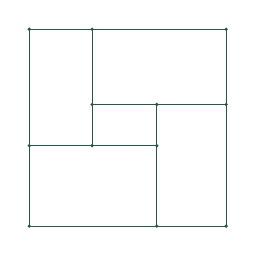
\begin{tikzpicture}[thachthuctoanhoc,scale=0.25]
			\draw [] (-5,5)-- (5,5);
			\draw [] (5,5)-- (5,-5);
			\draw [] (-5,5)-- (-5,-5);
			\draw [] (-5,-5)-- (5,-5);
			\draw [] (-1.8064850795005638,5)-- (-1.806485079500564,-0.9133587450621485);
			\draw [] (-5,-0.9133587450621485)-- (1.4776647785694939,-0.9133587450621485);
			\draw [] (1.4776647785694939,1.1789625354824862)-- (1.477664778569494,-5);
			\draw [] (-1.806485079500564,1.1789625354824862)-- (5,1.1789625354824862);
			\draw [fill=white] (-5,5) circle (1.5pt);
			\draw [fill=white] (5,5) circle (1.5pt);
			\draw [fill=white] (5,-5) circle (1.5pt);
			\draw [fill=white] (-5,-5) circle (1.5pt);
			\draw [fill=white] (-1.8064850795005638,5) circle (1.5pt);
			\draw [fill=white] (5,1.1789625354824862) circle (1.5pt);
			\draw [fill=white] (-5,-0.9133587450621485) circle (1.5pt);
			\draw [fill=white] (1.477664778569494,-5) circle (1.5pt);
			\draw [fill=white] (-1.806485079500564,1.1789625354824862) circle (1.5pt);
			\draw [fill=white] (1.4776647785694939,1.1789625354824862) circle (1.5pt);
			\draw [fill=white] (1.4776647785694939,-0.9133587450621485) circle (1.5pt);
			\draw [fill=white] (-1.806485079500564,-0.9133587450621485) circle (1.5pt);
		\end{tikzpicture}
		\vspace*{-10pt}
	\end{figure}
	Ký hiệu ${a_1},{a_2}, \ldots ,{a_{10}}$  là độ dài các cạnh của năm hình chữ nhật trong phân chia nói trên, như ở Hình $1$ dưới đây.
	\begin{figure}[H]
		\vspace*{-15pt}
		\centering
		\captionsetup{labelformat= empty, justification=centering}
		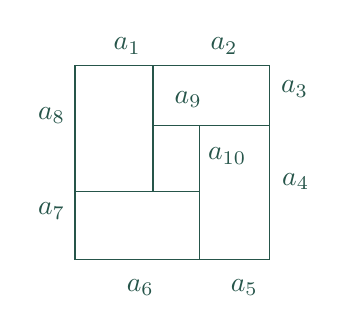
\begin{tikzpicture}[scale=0.495,thachthuctoanhoc]
			\draw  (0.,0.)-- (5.,0.);
			\draw  (0.,5.)-- (5.,5.);
			\draw  (5.,5.)-- (5.,0.);
			\draw  (0.,5.)-- (0.,0.);
			\draw  (2.,5.)-- (2.,1.76);
			\draw  (2.,1.76)-- (0.,1.76);
			\draw  (2.,3.46)-- (5.,3.46);
			\draw  (3.2,3.46)-- (3.2,0.);
			\draw  (2.,1.76)-- (3.2,1.76);
			\draw (0.7411478095238109,5.945053904761909) node[anchor=north west] {$a_1$};
			\draw (3.225934666666671,5.945053904761909) node[anchor=north west] {$a_2$};
			\draw (5.035841142857149,4.840704190476194) node[anchor=north west] {$a_3$};
			\draw (5.06651752380953,2.4786228571428586) node[anchor=north west] {$a_4$};
			\draw (3.7474331428571475,-0.2619525714285716) node[anchor=north west] {$a_5$};
			\draw (1.0785880000000017,-0.24233053333333336) node[anchor=north west] {$a_6$};
			\draw (-1.2,1.7117133333333343) node[anchor=north west] {$a_7$};
			\draw (-1.2,4.165823809523812) node[anchor=north west] {$a_8$};
			\draw (2.305643238095241,4.564616761904765) node[anchor=north west] {$a_9$};
			\draw (3.1645819047619086,3.1228268571428592) node[anchor=north west] {$a_{10}$};
		\end{tikzpicture}
		\caption{\small\textit{\color{thachthuctoanhoc}Hình $1$}}
		\vspace*{-15pt}
	\end{figure}
	Ta có $\left\{ {{a_1};{a_2}; \ldots ;{a_{10}}} \right\} = \left\{ {1;2; \ldots ;10} \right\},$ và
	\begin{align*}
		n = {a_1} + {a_2} = {a_3} + {a_4} = {a_5} + {a_6} = {a_7} + {a_8}.
	\end{align*}
	Do đó
	\begin{align*}
		4n &= {a_1} + {a_2} + {a_3} + {a_4} + {a_5} + {a_6} + {a_7} + {a_8} \\
		&\le 3 + 4 + 5 + 6 + 7 + 8 + 9 + 10 = 52;
	\end{align*}
	suy ra, $n \le 13$. Mà theo giả thiết, $n \ge 13$, nên $n = 13$.
	\vskip 0.05cm
	Như vậy, với $n \ge 13$, ta có thể phân chia hình vuông cạnh $n$ thành năm hình chữ nhật, thỏa mãn các yêu cầu của đề bài, chỉ khi $n = 13$.
	\vskip 0.05cm
	Với $n = 13$, phân chia được thể hiện ở Hình $2$ dưới đây thỏa mãn các yêu cầu của đề bài.
	\begin{figure}[H]
		\vspace*{-15pt}
		\centering
		\captionsetup{labelformat= empty, justification=centering}
		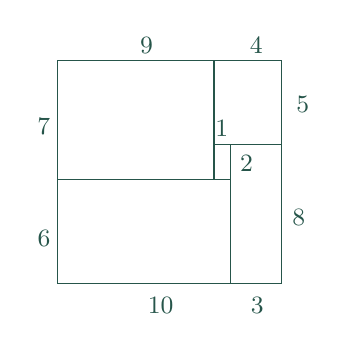
\begin{tikzpicture}[scale=0.22,thachthuctoanhoc, node font=\small]
			\draw  (0.,0.)-- (12.902720021180311,0.);
			\draw  (0.,12.902720021180311)-- (12.902720021180311,12.902720021180311);
			\draw  (12.902720021180311,12.902720021180311)-- (12.902720021180311,0.);
			\draw  (0.,12.902720021180311)-- (0.,0.);
			\draw  (9.025004744255101,12.902720021180313)-- (9.025004744255101,6.);
			\draw  (9.025004744255101,6.)-- (0.,6.);
			\draw  (9.025004744255101,8.033375486746607)-- (12.902720021180311,8.033375486746607);
			\draw  (10.,8.033375486746607)-- (10.,0.);
			\draw  (9.025004744255101,6.)-- (10.,6.);
			\draw (4.231659743459114,14.7289269960977) node[anchor=north west] {$9$};
			\draw (10.574639348977636,14.751598908646) node[anchor=north west] {$4$};
			\draw (13.261077770138423,11.311830988972293) node[anchor=north west] {$5$};
			\draw (8.58156796848920555,9.9755594148325) node[anchor=north west] {$1$};
			\draw (10.0126899612117505,7.9552898046145526) node[anchor=north west] {$2$};
			\draw (13.0186454480661734,4.795734936070321) node[anchor=north west] {$8$};
			\draw (10.6246248954267832,-0.25477887991443754) node[anchor=north west] {$3$};
			\draw (4.679399480319246,-0.25477887991443754) node[anchor=north west] {$10$};
			\draw (-1.68427239409557028,3.625632172873369) node[anchor=north west] {$6$};
			\draw (-1.69919705199090798,10.043235067868588) node[anchor=north west] {$7$};
		\end{tikzpicture}
		\caption{\small\textit{\color{thachthuctoanhoc}Hình $2$}}
		\vspace*{-15pt}
	\end{figure}
	Vậy, nếu $n = 13$ thì câu trả lời cho câu hỏi đặt ra ở bài toán là ``\textit{có thể}"; nếu $n > 13$ thì câu trả lời là ``\textit{không thể}".
	\vskip 0.05cm
	\textbf{\color{thachthuctoanhoc}Bình luận và Nhận xét}
	\vskip 0.05cm
	Trong số các lời giải Tạp chí nhận được từ bạn đọc, rất tiếc, có một lời giải sai (do người giải bài đã mắc khá nhiều lỗi logic trong các lập luận) và một lời giải không được chấp nhận là lời giải hoàn chỉnh, do có câu trả lời không chính xác cho câu hỏi của bài toán và mắc một số lỗi ``chính tả" trong các diễn đạt toán học.
	\vskip 0.05cm
	\hfill \textbf{\color{thachthuctoanhoc}Lê Huy}
	\vskip 0.05cm
	{\color{thachthuctoanhoc}{\usefont{T5}{qag}{b}{n} P667.}}
	(Mức $A$) Chứng minh rằng
	\begin{align*}
		8(x+y-1)^2-9xy(x+y-1)+xy\ge0
	\end{align*}
	với mọi $x,y\in[0;1]$. 
	\vskip 0.05cm
	\textbf{\color{thachthuctoanhoc}Lời giải} (\textit{của người chấm bài})\textbf{\color{thachthuctoanhoc}.}
	\vskip 0.05cm
	Đặt $a = \dfrac{x + y}{2}$; khi đó, bất đẳng thức của đề bài trở thành
	\begin{align*}
		4{\left( {2a - 1} \right)^2} + xy\left( {5 - 9a} \right) \ge 0. \tag{$1$}
	\end{align*}
	Vì $x, y \in [0; 1]$ nên $a \in [0; 1]$.
	\vskip 0.05cm
	Nếu  $0 \le a \le \dfrac{5}{9}$ thì bất đẳng thức ($1$) hiển nhiên đúng.
	\vskip 0.05cm
	Xét $\dfrac{5}{9} < a \le 1$.
	\vskip 0.05cm  
	Khi đó, $5 - 9a < 0.$ \hfill ($2$)
	\vskip 0.05cm
	Theo bất đẳng thức trung bình cộng -- trung bình nhân, ta có:
	\begin{align*}
		{a^2} = {\left( {\dfrac{{x + y}}{2}} \right)^2} \ge xy. \tag{$3$}
	\end{align*}
	Từ ($2$) và ($3$), suy ra
	\begin{align*}
			&4{\left( {2a - 1} \right)^2} + xy\left( {5 - 9a} \right) \\[-0.5ex]
			\ge \,&4{\left( {2a - 1} \right)^2} + {a^2}\left( {5 - 9a} \right)\\
		 = \,&4 - 16a + 21{a^2} - 9{a^3}\\[-0.5ex]
		= \,&\left( {1 - a} \right){\left( {2 - 3a} \right)^2} \ge 0\left( {{\text{do }}a \le 1} \right).
	\end{align*}
	Bất đẳng thức ($1$) được chứng minh; và vì thế, bất đẳng thức của bài ra được chứng minh.
	\vskip 0.05cm
	\textbf{\color{thachthuctoanhoc}Bình luận và Nhận xét}
	\vskip 0.05cm
	$\pmb{1.}$ Dễ dàng chứng minh được rằng, dấu ``$=$" ở bất đẳng thức của đề bài xảy ra khi và chỉ khi
	\begin{align*}
		\left( {x,y} \right) \in \left\{ {\left( {0,1} \right),\left( {1,0} \right),\left( {1,1} \right),\left( {\dfrac{2}{3},\dfrac{2}{3}} \right)} \right\}.
	\end{align*}
	$\pmb{2.}$ Bằng cách đặt $z = 2 - x - y$, có thể biến đổi bất đẳng thức của đề bài về bất đẳng thức Schur bậc ba
	\begin{align*}
		xyz \ge \left( {x + y - z} \right)\left( {y + z - x} \right)\left( {z + x - y} \right).
	\end{align*}
	Vì thế, có thể nói, bất đẳng thức của bài ra là một trường hợp đặc biệt của bất đẳng thức vừa nêu trên, khi $z = 2 - x - y$.
	\vskip 0.05cm
	$\pmb{3.}$ Trong số các lời giải Tạp chí đã nhận được từ bạn đọc, rất tiếc, có một số lời giải sai, do người giải bài đã nhầm lẫn chiều của các bất đẳng thức, hoặc thực hiện sai một số tính toán.
	\vskip 0.05cm
	\hfill \textbf{\color{thachthuctoanhoc}Võ Quốc Bá Cẩn}
	\vskip 0.05cm
	{\color{thachthuctoanhoc}{\usefont{T5}{qag}{b}{n} P668.}}
	(Mức $A$) Cho số nguyên $n\ge2$. Có $n$ con ếch nằm trên một trục số, tại $n$ điểm tuỳ ý, thuộc tập $2n$ điểm $1,2,\ldots,2n$. Vào cùng một thời điểm, mỗi con ếch đều nhảy đến một trong số $n$ điểm còn lại, thuộc tập $2n$ điểm vừa nêu, sao cho không có hai con nào cùng nhảy tới một điểm. Chứng minh rằng
	\vskip 0.05cm
	$a)$ Tổng khoảng cách $n$ con ếch đã nhảy không vượt quá $n^2$. 
	\vskip 0.05cm
	$b)$ Tồn tại một phương án nhảy của $n$ con ếch, sao cho tổng khoảng cách chúng đã nhảy đúng bằng $n^2$. 
	\vskip 0.05cm
	\textbf{\color{thachthuctoanhoc}Lời giải} (\textit{dựa theo lời giải của tác giả bài toán}).
	\vskip 0.05cm
	Lần lượt, theo thứ tự từ bé đến lớn, ký hiệu ${a_1},{a_2}, \ldots ,{a_n}$  là các điểm mà $n$ con ếch nằm ở thời điểm ban đầu.
	\vskip 0.05cm
	Với mỗi $i = 1, 2, \ldots, n$, gọi con ếch nằm ở điểm  $a_i$ là con ếch thứ $i$.
	\vskip 0.05cm
	Với mỗi $i = 1, 2, \ldots, n$, ký hiệu $b_i$  là điểm con ếch thứ $i$ nhảy đến.
	\vskip 0.05cm
	Theo giả thiết của bài ra,
	\begin{align*}
		&\left\{ {{a_1};{a_2}; \ldots ;{a_n};{b_1};{b_2}; \ldots ;{b_n}} \right\} \\[-0.5ex]
		= \,&\left\{ {1;2; \cdots ;2n} \right\}. \tag{$1$}
	\end{align*}
	Với mỗi $i = 1, 2, \ldots, n$, khoảng cách con ếch thứ $i$ đã nhảy là $\left| {{a_i} - {b_i}} \right|.$
	\vskip 0.05cm 
	Ký hiệu $S$ là tổng khoảng cách $n$ con ếch đã nhảy. Do với mọi $i = 1, 2, \ldots , n$,
	\begin{align*}
		\left| {{a_i} - {b_i}} \right| = \max \left\{ {{a_i},{b_i}} \right\} - \min \left\{ {{a_i},{b_i}} \right\},
	\end{align*}
	nên
	\begin{align*}
		S = \sum\limits_{i = 1}^n {\!\max \!\left\{ {{a_i},{b_i}} \right\}}  \!-\! \sum\limits_{i = 1}^n {\!\min\! \left\{ {{a_i},{b_i}} \right\}}.  \tag{$2$}
	\end{align*}
	$a)$ Do ($1$) nên
	\begin{align*}
		\sum\limits_{i = 1}^n {\max \left\{ {{a_i},{b_i}} \right\}}  &\!\le\! \left( {n \!+\! 1} \right) \!+\! \left( {n \!+\! 2} \right) \!+\!  \cdots  \!+\! 2n \\[-1.2ex]
		&= {n^2} + \sum\limits_{k = 1}^n k,  \tag{$3$}\\[-1ex]
	\sum\limits_{i = 1}^n {\min \left\{ {{a_i},{b_i}} \right\}}  &\ge \sum\limits_{k = 1}^n k. \tag{$4$}
\end{align*}
	Từ ($2$), ($3$) và ($4$), suy ra
	\begin{align*}
		S \le \left( {{n^2} + \sum\limits_{k = 1}^n k } \right) - \sum\limits_{k = 1}^n k  = {n^2}.
	\end{align*}
	Ta có điều phải chứng minh theo yêu cầu đề bài.
	\vskip 0.05cm
	$b)$ Lần lượt, theo thứ tự từ lớn đến bé, ký hiệu ${c_1},{c_2}, \ldots ,{c_n}$  là các phần tử của tập hợp
	\begin{align*}
		\left\{ {1;2; \ldots ;2n} \right\}\backslash \left\{ {{a_1};{a_2}; \ldots ;{a_n}} \right\}.
	\end{align*}
	Xảy ra hai trường hợp sau:
	\vskip 0.05cm
	$\diamond$ \textit{Trường hợp} $1$: $1 \le {a_1} < {a_2} < \cdots  < {a_n} \le n.$
	\vskip 0.05cm  
	Khi đó, $\left\{ {{c_1},{c_2}, \ldots ,{c_n}} \right\} \!=\! \left\{ {n \!+\! 1;n \!+\! 2; \ldots ;2n} \right\}\!.$  Do đó, với mọi $i = 1, 2, \ldots, n$,
	\begin{align*}
		\max \!\left\{\! {{a_i},{c_i}} \!\right\} \!=\! {c_i} \!\ge\! n \!+\! 1, \min\! \left\{\! {{a_i},{c_i}} \!\right\} \!=\! {a_i} \!\le\! n.
	\end{align*}
	$\diamond$ \textit{Trường hợp} $2$: Tồn tại $h \in \mathbb{N^*}$  sao cho  $1 \le {a_1} <  \cdots  < {a_h} \le n < {a_{h + 1}} <  \cdots  < {a_n} \le 2n.$ 
	\vskip 0.05cm
	Khi đó, ${c_1} >  \cdots  > {c_h} \ge n + 1 > {c_{h + 1}} >  \cdots  > {c_n} \ge 1.$ 
	\vskip 0.05cm
	Do đó, với mọi $i = 1, 2, \ldots , h$,
	\begin{align*}
		\max \!\left\{\! {{a_i},{c_i}} \!\right\} \!=\! {c_i} \!\ge\! n \!+\! 1, \min\! \left\{ \!{{a_i},{c_i}} \!\right\} \!=\! {a_i} \!\le\! n;
	\end{align*}
	và với mọi $i = h + 1, \ldots , n$,
	\begin{align*}
		\max\! \left\{\! {{a_i},{c_i}} \!\right\} \!=\! {a_i} \!\ge\! n \!+\! 1, \min\! \left\{\! {{a_i},{c_i}} \!\right\} \!=\! {c_i} \!\le\! n.
	\end{align*}
	Từ kết quả xét hai trường hợp trên, suy ra, ta luôn có
	\begin{align*}
		\max \!\left\{\! {{a_i},{c_i}} \!\right\} \!\ge\! n \!+\! 1,\min\! \left\{\! {{a_i},{c_i}} \!\right\} \!\le\! n, \tag{$5$}
	\end{align*}
	với mọi $i = 1, 2, \ldots, n$.
	\vskip 0.05cm
	Xét phương án nhảy như sau của $n$ con ếch: Với mỗi $i = 1, 2, \ldots, n$, $b_i = c_i$.
	\vskip 0.05cm  
	Khi đó, theo ($5$),
	\begin{align*}
		\max \!\left\{\! {{a_i},{b_i}} \!\right\} \!\ge\! n \!+\! 1,\min\! \left\{\! {{a_i},{b_i}} \!\right\} \!\le\! n,
	\end{align*}
	với mọi $i = 1, 2, \ldots , n$.
	\vskip 0.05cm
	Do đó, với lưu ý tới ($1$), ta có:
	\begin{align*}
		\sum\limits_{i = 1}^n {\max \left\{ {{a_i},{b_i}} \right\}}  &= \left( {n \!+\! 1} \right) \!+\! \left( {n \!+\! 2} \right) \!+\!  \cdots \! +\! 2n \\[-1.2ex]
		&= {n^2} + \sum\limits_{k = 1}^n k\\[-1.2ex]
		\sum\limits_{i = 1}^n {\min \left\{ {{a_i},{b_i}} \right\}}  &= \sum\limits_{k = 1}^n k.
	\end{align*}
	Vì thế, theo ($2$), $S = n^2$.
	\vskip 0.05cm  
	Ta có điều phải chứng minh theo yêu cầu đề bài.
	\vskip 0.05cm
	\textbf{\color{thachthuctoanhoc}Bình luận và Nhận xét}
	\vskip 0.05cm
	Tạp chí đã nhận được hai lời giải, từ bạn đọc; trong đó, rất tiếc, có một lời giải sai ở ý $b)$, do người giải bài, khi xây dựng phương án nhảy của $n$ con ếch, đã áp đặt vị trí ban đầu của chúng là $n$ điểm $1, 2, \ldots, n$.
	\vskip 0.05cm
	\hfill	\textbf{\color{thachthuctoanhoc}Nguyễn Khắc Minh}
	\vskip 0.05cm
	{\color{thachthuctoanhoc}{\usefont{T5}{qag}{b}{n} P669.}}
	(Mức $A$) Cho tam giác nhọn $ABC$, với $AB<AC$, nội tiếp đường tròn $(O)$. Gọi $M,N$ tương ứng là trung điểm của các cung $BC$ lớn và cung $BC$ nhỏ. Trên đường thẳng $AN$, lấy điểm $D$ sao cho $D$ nằm trong tam giác $ABC$ và không trùng với tâm đường tròn nội tiếp tam giác ấy. Trên đoạn thẳng $MD$, lấy điểm $T$ sao cho $\angle{MBT}=\angle{DCB}$. Chứng minh rằng trực tâm của tam giác $TND$ nằm trên đường thẳng $BC$.
	\vskip 0.05cm
	\textbf{\color{thachthuctoanhoc}Lời giải} (\textit{của người chấm bài}).
	\begin{figure}[H]
		\vspace*{-10pt}
		\centering
		\captionsetup{labelformat= empty, justification=centering}
		\definecolor{ffqqqq}{rgb}{1.,0.,0.}
		\definecolor{qqwuqq}{rgb}{0.,0.39215686274509803,0.}
		\definecolor{xdxdff}{rgb}{0.49019607843137253,0.49019607843137253,1.}
		\definecolor{uuuuuu}{rgb}{0.26666666666666666,0.26666666666666666,0.26666666666666666}
		\definecolor{qqqqff}{rgb}{0.,0.,1.}
		\begin{tikzpicture}[scale=0.32,thachthuctoanhoc]
			\draw [shift={(10.,-2.)},pattern color=qqwuqq,fill=qqwuqq,fill opacity=0.10000000149011612] (0,0) -- (166.8046508068974:0.88) arc (166.8046508068974:180.:0.88) -- cycle;
			\draw [shift={(0.,-2.)},pattern color=qqwuqq,fill=qqwuqq,fill opacity=0.10000000149011612] (0,0) -- (44.4249154392908:0.88) arc (44.4249154392908:57.6202646323934:0.88) -- cycle;
			\draw[pattern color=qqwuqq,fill=qqwuqq,fill opacity=0.10000000149011612] (3.028672358412081,-4.746051562850727) -- (3.0941777880108416,-4.441898577178908) -- (2.790024802339022,-4.376393147580148) -- (2.7245193727402617,-4.680546133251967) -- cycle; 
			\draw [shift={(4.185301543683374,2.1021169441445613)},pattern color=qqwuqq,fill=qqwuqq,fill opacity=0.10000000149011612] (0,0) -- (-135.5750845607092:0.66) arc (-135.5750845607092:-102.15414161359068:0.66) -- cycle;
			\draw [shift={(10.,-2.)},pattern color=qqwuqq,fill=qqwuqq,fill opacity=0.10000000149011612] (0,0) -- (166.8046508068974:0.66) arc (166.8046508068974:200.22559375401596:0.66) -- cycle;
			\draw [shift={(2.7245193727402617,-4.680546133251967)},pattern color=qqwuqq,fill=qqwuqq,fill opacity=0.10000000149011612] (0,0) -- (20.225593754015947:0.66) arc (20.225593754015947:77.84585838640933:0.66) -- cycle;
			\draw [shift={(2.7245193727402617,-4.680546133251967)},pattern color=qqwuqq,fill=qqwuqq,fill opacity=0.10000000149011612] (0,0) -- (77.84585838640933:0.44) arc (77.84585838640933:135.4661230188027:0.44) -- cycle;
			\draw[pattern color=ffqqqq,fill=ffqqqq,fill opacity=0.10000000149011612] (2.662862274480868,1.6530470327261946) -- (2.7508851876612797,1.354631271153127) -- (3.049300949234347,1.442654184333539) -- (2.961278036053935,1.7410699459066064) -- cycle; 
			\draw  (2.,5.)-- (0.,-2.);
			\draw  (0.,-2.)-- (10.,-2.);
			\draw  (10.,-2.)-- (2.,5.);
			\draw  (5.,0.35714285714285715) circle (5.527759261127387cm);
			\draw  (5.,-5.17061640398453)-- (2.,5.);
			\draw  (3.6238019594012094,-0.505022281702721)-- (10.,-2.);
			\draw  (5.,5.884902118270244)-- (3.6238019594012094,-0.505022281702721);
			\draw  (5.,5.884902118270244)-- (0.,-2.);
			\draw  (4.185301543683374,2.1021169441445613)-- (0.,-2.);
			\draw (1.3538,6.796) node[anchor=north west] {$A$};
			\draw (-0.64,-2.228) node[anchor=north west] {$B$};
			\draw (10.008,-1.728) node[anchor=north west] {$C$};
			\draw (4.64,7.242) node[anchor=north west] {$M$};
			\draw (4.75,-4.984) node[anchor=north west] {$N$};
			\draw (4.992,0.626) node[anchor=north west] {$O$};
			\draw (3.1,-0.21) node[anchor=north west] {$D$};
			\draw (3.7266,2.804) node[anchor=north west] {$T$};
			\draw (2.0286,-4.722) node[anchor=north west] {$K$};
			\draw  (3.6238019594012094,-0.505022281702721)-- (2.7245193727402617,-4.680546133251967);
			\draw  (4.185301543683374,2.1021169441445613)-- (5.,-5.17061640398453);
			\draw  (4.185301543683374,2.1021169441445613)-- (-9.72171775070981,-2.);
			\draw  (5.,-5.17061640398453)-- (5.,5.884902118270244);
			\draw (-10.43,-1.954) node[anchor=north west] {$H$};
			\draw  (-9.72171775070981,-2.)-- (5.,-5.17061640398453);
			\draw  (-9.72171775070981,-2.)-- (0.,-2.);
			\draw  (2.7245193727402617,-4.680546133251967)-- (10.,-2.);
			\draw  (2.7245193727402617,-4.680546133251967)-- (0.,-2.);
			\draw  (5.,-5.17061640398453)-- (10.,-2.);
			\draw [shift={(4.185301543683374,2.1021169441445613)},color=qqwuqq] (-135.5750845607092:0.66) arc (-135.5750845607092:-102.15414161359068:0.66);
			\draw [shift={(4.185301543683374,2.1021169441445613)},color=qqwuqq] (-135.5750845607092:0.55) arc (-135.5750845607092:-102.15414161359068:0.55);
			\draw [shift={(10.,-2.)},color=qqwuqq] (166.8046508068974:0.66) arc (166.8046508068974:200.22559375401596:0.66);
			\draw [shift={(10.,-2.)},color=qqwuqq] (166.8046508068974:0.55) arc (166.8046508068974:200.22559375401596:0.55);
			\draw [shift={(2.7245193727402617,-4.680546133251967)},color=qqwuqq] (20.225593754015947:0.66) arc (20.225593754015947:77.84585838640933:0.66);
			\draw[color=qqwuqq] (3.113938829900631,-4.232005737763528) -- (3.20047648704738,-4.132330094321653);
			\draw [shift={(2.7245193727402617,-4.680546133251967)},color=qqwuqq] (77.84585838640933:0.44) arc (77.84585838640933:135.4661230188027:0.44);
			\draw[color=qqwuqq] (2.6173217256447794,-4.322238075210854) -- (2.5794872619640197,-4.195776407666933);
			\draw  (-9.72171775070981,-2.)-- (3.6238019594012094,-0.505022281702721);
			\draw  (0.,-2.)-- (5.,-5.17061640398453);
			\draw [fill=white] (2.,5.) circle (1.5pt);
			\draw [fill=white] (0.,-2.) circle (1.5pt);
			\draw [fill=white] (10.,-2.) circle (1.5pt);
			\draw [fill=white] (5.,0.35714285714285715) circle (1.5pt);
			\draw [fill=white] (5.,-5.17061640398453) circle (1.5pt);
			\draw [fill=white] (5.,5.884902118270244) circle (1.5pt);
			\draw [fill=white] (3.6238019594012094,-0.505022281702721) circle (1.5pt);
			\draw [fill=white] (0.,-2.) circle (1.5pt);
			\draw [fill=white] (0.,-2.) circle (1.5pt);
			\draw [fill=white] (4.185301543683374,2.1021169441445613) circle (1.5pt);
			\draw [fill=white] (5.,5.884902118270244) circle (1.5pt);
			\draw [fill=white] (2.7245193727402617,-4.680546133251967) circle (1.5pt);
			\draw [fill=white] (-9.72171775070981,-2.) circle (1.5pt);
		\end{tikzpicture}
		\vspace*{-20pt}
	\end{figure}
	Gọi $K$ là giao điểm thứ hai, khác $M$, của $MD$ và $(O)$.
	\vskip 0.05cm
	Do $M$ là điểm chính giữa cung $BAC$ nên
	\begin{align*}
		\angle BKT \!=\! \angle BKM \!=\! \angle MKC \!=\! \angle DKC. \tag{$1$}
	\end{align*}
	Do $BKCM$ là tứ giác nội tiếp, nên $\angle BMK = \angle BCK$; kết hợp với giả thiết $\angle MBT = \angle DCB,$  suy ra
	\begin{align*}
		\angle BTK &= \angle MBT + \angle BMK \\
		&= \angle DCB + \angle BCK = \angle DCK. \tag{$2$}
	\end{align*}
	Từ ($1$) và ($2$), suy ra $\Delta BKT \sim  \Delta DKC$; do đó
	\begin{align*}
		\dfrac{{KB}}{{KT}} = \dfrac{{KD}}{{KC}}. \tag{$3$}
	\end{align*}
	Gọi $H$ là giao điểm của $NK$ và $BC$.
	\vskip 0.05cm
	Từ giả thiết về vị trí của các điểm $M$, $N$, suy ra $MN$ là đường kính của $(O)$. Do đó, $KN \bot KM$; mà $KM$ là phân giác trong của góc $BKC$ (vì $M$ là điểm chính giữa cung $BAC$), nên $KN$ là phân giác ngoài của góc $BKC$. Suy ra, $\angle NKC = \angle BKH$. \hfill ($4$)
	\vskip 0.05cm 
	Vì $BKNC$ là tứ giác nội tiếp, nên 
	\begin{align*}
		\angle KNC = \angle KBH. \tag{$5$}
	\end{align*}
	Từ ($4$) và ($5$), suy ra $\Delta NKC \sim \Delta BKH$; do đó
	\begin{align*}
		\dfrac{{KC}}{{KN}} = \dfrac{{KH}}{{KB}}. \tag{$6$}
	\end{align*}
	Từ ($3$) và ($6$), suy ra
	\begin{align*}
		\dfrac{{KH}}{{KT}} = \dfrac{{KH}}{{KB}} \cdot \dfrac{{KB}}{{KT}} = \dfrac{{KC}}{{KN}} \cdot \dfrac{{KD}}{{KC}} = \dfrac{{KD}}{{KN}}.
	\end{align*}
	Mà  $\angle TKH = \angle NKD = {90^{\rm{o}}}$ (do $KN \bot KM$, theo chứng minh trên), nên $\Delta KHT \sim  \Delta KDN$. Suy ra
	\begin{align*}
		\angle THK = \angle NDK = {90^{\rm{o}}} - \angle KND.
	\end{align*}
	Do đó
	\begin{align*}
		\angle THN + \angle HND = \angle THK + \angle KND = {90^\circ}.
	\end{align*}
	Suy ra, $TH \bot ND$. Mà $NH \bot TD$ (do $KN \bot KM$, theo chứng minh trên), nên $H$ là trực tâm của tam giác $TND$. Vì vậy, trực tâm của tam giác $TND$ nằm trên đường thẳng $BC$.
	\vskip 0.05cm
	Ta có điều phải chứng minh theo yêu cầu đề bài.
	\vskip 0.05cm
	\textbf{\color{thachthuctoanhoc}Bình luận và Nhận xét}
	\vskip 0.05cm
	Trong số các lời giải Tạp chí đã nhận được từ bạn đọc, có một lời giải không được chấp nhận là lời giải đúng, do người giải bài đã sử dụng chưa đúng một dấu hiệu nhận biết trực tâm của một tam giác.
	\begin{flushright}
		\textbf{\color{thachthuctoanhoc}Hạ Vũ Anh}
	\end{flushright}
	{\color{thachthuctoanhoc}{\usefont{T5}{qag}{b}{n} P670.}}
	(Mức $A$) Hỏi, có thể chọn được tối đa bao nhiêu điểm nguyên trong mặt phẳng toạ độ, sao cho đoạn thẳng nối hai điểm bất kỳ trong chúng chứa đúng $2022$ điểm nguyên?
	\vskip 0.05cm
	(Trong mặt phẳng toạ độ, một điểm được gọi là {\it điểm nguyên}, nếu cả hoành độ và tung độ của nó đều là các số nguyên.)
	\vskip 0.05cm
	\textbf{\color{thachthuctoanhoc}Lời giải} (\textit{của người chấm bài})\textbf{\color{thachthuctoanhoc}.}
	\vskip 0.05cm
	Trong phần trình bày dưới đây, $\gcd(a, b)$ ký hiệu ước chung lớn nhất của hai số nguyên $a, b$.\vskip 0.05cm
	Trước hết, ta nhắc lại kết quả quen biết sau:
	\vskip 0.05cm
	\textbf{\color{thachthuctoanhoc}Bổ đề.} Trong mặt phẳng tọa độ $Oxy$, cho hai điểm nguyên phân biệt $A(a, b)$ và $B(u, v)$. Khi đó, số điểm nguyên thuộc đoạn thẳng $AB$ bằng $\gcd(a - u, b - v) + 1$.
	\vskip 0.05cm
	\textit{Chứng minh.}
	\vskip 0.05cm
	Không mất tính tổng quát, giả sử $b \ge  v$.
	\vskip 0.05cm
	Xét phép tịnh tiến theo vectơ $\overrightarrow{BO}$. Qua phép tịnh tiến này, điểm $A$ biến thành điểm $A'\left( {a - u,b - v} \right),$  và điểm $B$ biến thành gốc tọa độ $O$. Dễ thấy, số điểm nguyên thuộc đoạn thẳng $AB$ bằng số điểm nguyên thuộc đoạn thẳng $OA'$.
	\vskip 0.05cm 
	Gọi $s$ là số điểm nguyên thuộc đoạn thẳng $OA'$.
	\vskip 0.05cm
	Do $b \ge  v$ nên xảy ra hai trường hợp sau:
	\vskip 0.05cm
	$\diamond$ \textit{Trường hợp} $1$: $b = v$.
	\vskip 0.05cm
	Khi đó, $A'$  là điểm nằm trên trục hoành, và có hoành độ là $a - u$. Vì vậy
	\begin{align*}
		s = (a - u) + 1 &= \gcd(a - u, 0) + 1 \\
		&= \gcd(a - u, b - v) + 1.
	\end{align*}
	$\diamond$ \textit{Trường hợp} $2$: $b > v$.
	\vskip 0.05cm
	Đặt $d = \gcd(a - u, b - v)$.
	\vskip 0.05cm
	Khi đó, tồn tại $c\in \mathbb{Z}$  và $k \in \mathbb{N^*}$  nguyên tố cùng nhau, sao cho
	\begin{align*}
		a - u = cd \text{ và } b - v = kd.
	\end{align*}
	Xảy ra hai trường hợp sau:
	\vskip 0.05cm
	$+$ \textit{Trường hợp} $2.1$: $a = u$.
	\vskip 0.05cm
	Khi đó, $A'$  là điểm nằm trên trục tung, và có tung độ là $b - v$. Vì thế
	\begin{align*}
		s = (b - v) + 1 &= \gcd(0, b - v) + 1 \\
		&= \gcd(a - u, b - v) + 1.
	\end{align*}
	$+$ \textit{Trường hợp} $2.2$: $a \ne u$.
	\vskip 0.05cm
	Khi đó, $c \ne 0$; do đó, đường thẳng $OA'$  có phương trình:
	\begin{align*}
		y = \frac{k}{c}x.
	\end{align*}
	Vì thế, với điểm $M\left( {{x_M},{y_M}} \right)$  tùy ý thuộc đoạn thẳng $OA'$,  ta có $0 \le {y_M} \le kd,$  và
	\begin{align*}
		{y_M} = \frac{k}{c}{x_M}.
	\end{align*}
	Từ đó, do $\gcd(c, k) = 1$, suy ra, điểm  $M\left( {{x_M},{y_M}} \right)$ thuộc đoạn thẳng  $OA'$ là điểm nguyên khi và chỉ khi $x_M = hc$,  với $h$ là số tự nhiên thỏa mãn $0 \le h \le d$. Vì vậy
	\begin{align*}
		s = d + 1 = \gcd(a - u, b - v) + 1.
	\end{align*}
	Kết quả xét các trường hợp nêu trên cho ta điều phải chứng minh theo yêu cầu của Bổ đề.
	\vskip 0.05cm
	\textit{Trở lại bài toán.}
	\vskip 0.05cm
	Xét số nguyên dương $n$, mà với nó, tồn tại $n$ điểm phân biệt  ${A_1}\left( {{x_1},{y_1}} \right),$ ${A_2}\left( {{x_2},{y_2}} \right), \ldots ,$ ${A_n}\left( {{x_n},{y_n}} \right)$, sao cho đoạn thẳng nối hai điểm bất kỳ trong chúng chứa đúng $2022$ điểm nguyên.
	\vskip 0.05cm
	Khi đó, theo Bổ đề,
	\begin{align*}
		\gcd \left( {{x_i} - {x_j},{y_i} - {y_j}} \right) = 2021, \tag{$1$}
	\end{align*}
	với mọi $i, j \in \{1; 2; \ldots ; n\}, i \ne j$.
	\vskip 0.05cm
	Với mỗi $i = 1, 2, \ldots , n$, gọi $r_i$  và $s_i$  tương ứng là số dư trong phép chia $x_i$  và $y_i$  cho $2$.
	\vskip 0.05cm
	Khi đó, do  ${r_i},{s_i} \in \left\{ {0;1} \right\}$ với mọi \linebreak$i \in \{1; 2; \ldots ; n\}$, nên
	\begin{align*}
		\left( {{r_i},{s_i}} \right) \in \left\{ {\left( {0,0} \right);\left( {0,1} \right);\left( {1,0} \right);\left( {1,1} \right)} \right\}
	\end{align*}
	với mọi $i \in \{1; 2; \ldots ; n\}$.
	\vskip 0.05cm
	Vì thế, nếu $n \ge  5$ thì theo nguyên lý Dirichlet, tồn tại $p \ne q, p, q \in \{1; 2; \ldots ; n\}$, sao cho
	\begin{align*}
		\left( {{r_p},{s_p}} \right) = \left( {{r_q},{s_q}} \right).
	\end{align*}
	Nghĩa là, tồn tại $p \ne q, p, q \in \{1; 2; \ldots ; n\}$, sao cho 
	\begin{align*}
		{x_p} \equiv {x_q}\left( {\bmod 2} \right) \text{ và } {y_p} \equiv {y_q}\left( {\bmod 2} \right). \tag{$2$}
	\end{align*}
	Từ ($2$) và ($1$), suy ra
	\begin{align*}
		2\left| {\gcd \left( {{x_p} - {x_q},{y_p} - {y_q}} \right) = 2021,} \right.
	\end{align*}
	là điều vô lý. Vì vậy, $n \le 4$.
	\vskip 0.05cm
	Hơn nữa, bằng cách sử dụng Bổ đề, dễ dàng chứng minh được rằng, đoạn thẳng, nối hai điểm bất kỳ trong bốn điểm $A(0, 0),$ $B(0, 2021),$ $C(2021, 0),$ $D(2021, 2021)$, chứa đúng $2022$ điểm nguyên.
	\vskip 0.05cm
	Vậy, có thể chọn được tối đa bốn điểm nguyên trong mặt phẳng tọa độ, sao cho đoạn thẳng nối hai điểm bất kỳ trong chúng chứa đúng $2022$ điểm nguyên.
	\vskip 0.05cm
	\textbf{\color{thachthuctoanhoc}Bình luận và Nhận xét}
	\vskip 0.05cm
	$\pmb{1.}$ Lời giải trên cho thấy, bài đã ra là một khai thác nhẹ nhàng, thú vị đối với một kết quả cơ bản, quen biết về lưới nguyên trong mặt phẳng (Bổ đề trong lời giải trên).
	\vskip 0.05cm
	$\pmb{2.}$ Ở lời giải trên, thay $2021$ bởi $2n - 1$, $2022$ bởi $2n$, và $n$ bởi $m$, ta sẽ thu được một chứng minh cho khẳng định sau:
	\vskip 0.05cm
	``\textit{Với mọi số nguyên dương $n$, luôn chọn được tối đa bốn điểm nguyên trong mặt phẳng tọa độ, sao cho đoạn thẳng nối hai điểm bất kỳ trong chúng chứa đúng $2n$ điểm nguyên.}"
	\vskip 0.05cm
	$\pmb{3.}$ Trong số các lời giải Tạp chí nhận được từ bạn đọc, rất tiếc, có hai lời giải không được chấp nhận là lời giải hoàn chỉnh, do trong các lời giải đó có một số lập luận không chặt chẽ, thiếu chính xác.
	\begin{flushright}
		\textbf{\color{thachthuctoanhoc}Nguyễn Khắc Minh}
	\end{flushright}
\end{multicols}


%	\newpage 
%
%	\setcounter{figure}{0}
%	\thispagestyle{cackithitoannone}
\pagestyle{cackithitoan}
\everymath{\color{cackithi}}
\graphicspath{{../cackithi/pic/}}
\begingroup
\AddToShipoutPicture*{\put(0,616){\includegraphics[width=19.3cm]{../bannercackithi}}}
\AddToShipoutPicture*{\put(45,530){\includegraphics[scale=0.95]{../tieude.pdf}}}
\centering
\endgroup
\vspace*{175pt}

\begin{multicols}{2}
	Kỳ thi chọn học sinh giỏi quốc gia môn Toán THPT năm học $2022-2023$ được diễn ra trong hai ngày $24$ và $25/2/2023$ với xấp xỉ $500$ thí sinh tham gia dự thi. Kết quả kỳ thi được công bố vào chiều tối ngày $13/3/2023$. Trong bài viết này, chúng tôi xin đưa ra một số tổng kết, đánh giá và bình luận về đề thi và kết quả của kỳ thi năm nay.
	\vskip 0.05cm
	\textbf{\color{cackithi}Về đề thi}
	\vskip 0.05cm
	Đề thi năm nay vẫn giữ ổn định cấu trúc đề thi HSG quốc gia môn toán từ gần $15$ năm nay.
	Ngày thứ nhất bốn bài toán lần lượt thuộc các phân môn: giải tích, số học, đại số và hình học. Bài toán giải tích là một bài toán thuộc chủ đề quen thuộc: giới hạn dãy số. Ý đầu ở mức căn bản sử dụng tính chất dãy đơn điệu và bị chặn thì có giới hạn, còn ý sau liên quan đến khảo sát dãy số ở dạng tích bằng cách logarit hóa. Việc sử dụng phép thế lượng giác chỉ giúp nhìn ra vấn đề nhanh hơn và giải gọn hơn chứ không phải là cách giải tiên quyết. Có thể đánh giá đây là bài dễ nhất của ngày thứ nhất cũng là bài dễ nhất của cả hai ngày. 
	\vskip 0.05cm
	Ở Bài $2$, bài số học, thì ý đầu là một ý hoàn toàn đại số và rất cơ bản, chúng ta có thể tìm được công thức tổng quát của dãy số một cách dễ dàng. Phần chính của bài toán này là ý sau (không liên quan gì đến ý đầu). Yêu cầu bài toán được phát biểu khá thú vị, thoạt nhìn thì có vẻ rất ``khủng" nhưng nếu xem kỹ về bản chất thì khá đơn giản, chỉ dùng đến nguyên lý Dirichlet và tính tuần hoàn của số dư của dãy truy hồi nguyên. 
	\vskip 0.05cm
	Bài $3$ là một bài về bất đẳng thức ba biến có điều kiện, có thể nói là có dạng khá quen thuộc. Hướng đi tự nhiên nhất của bài này là chuẩn hóa rồi đưa về một biến (cụ thể là biến $r = abc$). Như vậy, xét về độ khó thì bài $3$ nhẹ nhàng hơn Bài $2$ cả về phát biểu (rất dễ hiểu), hướng đi và kỹ thuật.  
	\vskip 0.05cm
	Bài $4$ là một bài toán hình học có hai ý gần như độc lập. Ý đầu có điểm mấu chốt là có được $AKJH$ là hình bình hành rồi dùng tứ giác nội tiếp hoặc hàng điểm điều hoàn. Ý sau dùng tính chất của đường thẳng Simson và phép vị tự sẽ làm khá gọn. 
	\vskip 0.05cm
	Đánh giá sơ bộ cho đề thi ngày $1$ là đề khá dài, có nhiều ý, đặc biệt là các ý trong các Bài $2$ và $4$ hầu như không lên quan đến nhau. Các ý khó là $2b$ và $4a$, $4b$.
	\vskip 0.05cm 
	Đề thi ngày thứ hai gồm $3$ bài toán thuộc ba phân môn, lần lượt là: đại số, tổ hợp, hình học.
	\vskip 0.05cm
	Bài $5$ là một bài phương trình hàm có dạng giống (và cách giải cũng tương tự) với một bài toán trong IMO shortlist $2000$, khai thác tính toàn ánh và đơn ánh của phương trình hàm có biến nằm ngoài biểu thức hàm số. Không khó về mặt ý tưởng nhưng đây vẫn là một thách thức lớn cho thí sinh với những khó khăn kỹ thuật.   
	\vskip 0.05cm
	Bài $6$ là một bài toán tổ hợp về họ tập con khá quen thuộc sử dụng phương pháp đếm bằng hai cách. Dạng toán này đã xuất hiện nhiều, chỉ là với các tham số khác. Có lẽ khó khăn lớn nhất trong bài này là việc xây dựng ví dụ (nhất là trong tình huống các đánh giá đưa ra mới chỉ là các điều kiện cần). Phát biểu của bài toán này cũng hơi rối rắm và có lẽ điều đó cũng làm cho số thí sinh làm tốt bài này không nhiều.
	\vskip 0.05cm
	Bài $7$ là một bài toán hình học có cấu hình khá phức tạp với ý đầu là một bất đẳng thức hình học và ý sau yêu cầu chứng minh tính chất hình học thuần túy. Ý đầu có thể giải quyết khá gọn nếu biết một bổ đề quen thuộc sau: Cho góc xAy. Đường tròn $(I)$ tiếp xúc $Ax$, $Ay$ tại $B$, $C$. Đường tròn $(J)$ qua $A$ tiếp xúc $(I)$ cắt $Ax$, $Ay$ tại $D$, $E$. Khi đó $AD + AE \ge BC$. Ý sau tuy có vẻ rối rắm nhưng lại có nhiều hướng để tiếp cận.
	\vskip 0.05cm
	So với ngày thứ nhất thì đề thi ngày thứ hai cân bằng hơn: Bài $6$ với hai ý $6a$, $6b$ khá nhẹ nhàng, Bài $5$ cũng có ý $5a$ cơ bản, còn lại các ý khó là $5b$, $6c$ và bài hình. 
	\vskip 0.05cm
	Về tổng thể đề thi năm nay được đánh giá là khó, dài với nhiều ý (hầu như bài nào cũng có ý $a$, $b$, thậm chí $c$), hơi nặng về kỹ thuật, phần hình học khá nặng với hai bài, bốn ý riêng biệt, cấu hình rất phức tạp và đều đặt ở vị trí bài cuối (và quả thật cũng là bài khó của từng ngày).
	\vskip 0.05cm
	\textbf{\color{cackithi}Về kết quả}
	\vskip 0.05cm
	Trước hết là điểm chuẩn. Dù đề thi năm nay được đánh giá là khá khó, dài và nhiều ý, nhưng điểm chuẩn không quá thấp như dự đoán ban đầu: KK -- $13{,}5$; Ba: $16{,}5$; Nhì: $20{,}5$; Nhất $28$ và điểm để dự thi chọn đội tuyển là $23$. 
	\vskip 0.05cm
	Kết quả tốt nhất thuộc về đội tuyển Hà Tĩnh với hai giải nhất, tám giải nhì. Trong đó có em Trần Minh Hoàng, học sinh lớp $10$ chuyên Hà Tĩnh đạt thủ khoa với số điểm $32$ (với một đề thi có đến năm bài ở mức khó thì đây là một kết quả tuyệt vời đối với một bạn học sinh lớp $10$).
	\vskip 0.05cm
	Tiếp theo là đội tuyển Phú Thọ với hai giải nhất, năm giải nhì, ba giải ba. Đội tuyển trường PTNK, ĐHQG--HCM vẫn giữ được phong độ với hai giải nhất, ba giải nhì, hai giải ba và hai giải KK. 
	\vskip 0.05cm
	Ngoài ba đơn vị dẫn đầu có hai giải nhất, các đơn vị có giải nhất và cũng có kết quả tốt là: ĐHKHTN, ĐQGHN: một giải nhất, ba nhì, ba giải ba; Bắc Ninh: một giải nhất, hai giải nhì, năm giải ba; Hà Nội, một giải nhất, ba giải nhì, bốn giải ba, sáu giải KK; Hải Phòng: một giải nhất, ba giải nhì, hai giải ba, hai giải KK; Thừa Thiên Huế: một giải nhất, một giải ba, bốn giải KK.
	\vskip 0.05cm
	Đây đều là các đơn vị có truyền thống của VMO. Ở một góc nhìn khác, VMO năm nay có những đơn vị có những thành tích vượt bậc so với chính mình như Sóc Trăng có một giải nhì, một giải ba, hai giải KK; Lâm Đồng có hai giải nhì, một giải ba, một giải KK; Điện Biên có hai giải ba, Trà Vinh có một giải nhì, Kiên Giang có một giải  ba, một giải KK. Đặc biệt, có hai bạn không phải là học sinh trường chuyên cũng đã xuất sắc đạt giải: một bạn học sinh THPT FPT Cần Thơ đạt giải ba và một bạn học sinh THCS \& THPT Đông Du Đăk lak đạt giải khuyến khích. 
	\vskip 0.05cm
	Cuối cùng xin được điểm qua về bản đồ TST năm nay. Với điểm chuẩn là $23$ có $48$ bạn đạt mốc điểm này, được phân bổ như sau: đông đảo nhất là Hà Tĩnh với tám bạn, tiếp đến là Phú Thọ với năm bạn. Năm đội mạnh tiếp theo, mỗi đội có ba học sinh gồm PTNK, ĐHQG--HCM; KHTN, ĐHQG--HN, ĐHSP HN, Hà Nội, Hải Phòng; các đội có hai thí sinh tham dự TST gồm Bắc Ninh, Nam Định, Nghệ An và Thanh Hóa. Cuối cùng là nhóm các đơn vị có một suất TST: Bà Rịa -- Vũng Tàu, Bắc Giang, Đà Nẵng, Hải Dương, Hưng Yên, Lâm Đồng, Quảng Bình, Quảng Ngãi, Quảng Ninh, Tp HCM, Thừa Thiên -- Huế và Trà Vinh. $48$ em này sẽ cùng với bạn Phạm Việt Hưng, HCV IMO $2022$, tranh sáu suất dự IMO $2023$ tại Nhật Bản. 
	\vskip 0.05cm
	Trong các suất dự TST chúng tôi đặc biệt muốn nhắc tới hai suất của Trà Vinh và Lâm Đồng. Với Trà Vinh, có lẽ đây là suất TST đầu tiên còn với Lâm Đồng thì điều đặc biệt là suất TST này thuộc về học sinh trường chuyên Bảo Lộc, một trường chuyên thứ hai trong tỉnh mới được thành lập sau này. Và bạn học sinh đạt giải nhì có điểm số rất cao, $27$ điểm, tức là chỉ thiếu tí chút là đạt giải nhất.
	\vskip 0.05cm
	Nói câu chuyện về các trường hợp FPT Cần Thơ, Đông Du Đak lak, Điện Biên, Kiên Giang, Sóc Trăng, Trà Vinh hay chuyên Bảo Lộc để thấy rằng ở đâu cũng có học sinh có tố chất tốt, chỉ cần có những người thầy tâm huyết, biết thổi vào học trò sự tự tin và niềm đam mê. Ở thời đại của Internet, đặc biệt với sự cởi mở của cộng đồng toán, các vấn đề về tài liệu, thông tin sẽ không còn là lợi thế của riêng ai, và, với hình thức học online, các bạn học sinh ở mọi miền đều có cơ hội được học với các thầy giáo, các chuyên gia giỏi. Cơ hội được học hỏi đồng đều hơn và cơ hội thành công cũng đồng đều hơn.
	\vskip 0.05cm
	\textbf{\color{cackithi}Một số bình luận và đề xuất}
	\vskip 0.05cm
	Trước hết là về đề thi. Với thời gian $180$ phút làm bài, đề thi như vậy là quá dài với quá nhiều ý, quá nhiều yêu cầu, đặc biệt là ở ngày thi thứ nhất. Đề thi học sinh giỏi đa số là những bài mới, đòi hỏi thí sinh phải có nhiều thời gian suy nghĩ, tìm hướng tiếp cận rồi mới đến giai đoạn xử lý kỹ thuật, rồi lại phải trình bày chặt chẽ. Và kỹ thuật cũng không đơn giản (trên thực tế, hai bài toán có hướng đi khá rõ ràng là bài bất đẳng thức và bài phương trình hàm đã gây rất nhiều khó khăn cho các bạn học sinh). Theo ý kiến của chúng tôi, nên hạn chế các đề toán có nhiều ý mà chỉ nên đưa ra yêu cầu xử lý trọn vẹn một vấn đề. Nếu bài toán có hai ý trở lên thì nhất thiết chúng phải liên quan đến nhau và ý đầu sẽ như một gợi ý cho ý sau.
	\vskip 0.05cm
	Một vấn đề nữa nên có sự thay đổi là số lượng bài của mỗi ngày. Hiện nay, với cấu trúc ($4+3$) thì ngày thứ nhất có bốn bài toán, mỗi bài được $5$ điểm còn ngày thứ hai có ba bài toán, mỗi bài được $6$ hoặc $7$ điểm. Rõ ràng ngày thứ nhất sẽ có nhiều áp lực hơn vì trên thực tế, độ khó của các bài toán của hai ngày không có sự chênh lệch đáng kể. Đã thế điểm số tối đa của mỗi bài ở ngày thứ nhất chỉ là $5$ điểm (có thể tưởng tượng lấy được $5$ điểm ở bài $2$ hay bài $4$ khó thế nào). Vì vậy, chúng tôi đề xuất nên quay lại định dạng ba bài mỗi ngày như giai đoạn trước năm $2007$, cũng là một định dạng quen thuộc của nhiều kỳ thi toán trên thế giới. Với định dạng sáu bài thì trong hai ngày như vậy, phân bổ cho mỗi phân môn một bài và một bài ở dạng kiến thức tổng hợp. Như vậy sẽ đều hơn thay vì hơi nặng về hình học và đại số như hiện nay. 
	\vskip 0.05cm
	Cuối cùng, để tiếp nối ý đã trình bày ở cuối phần $2$, chúng tôi đề xuất nên triển khai mạnh hơn nữa các hoạt động dạy, bồi dưỡng chung cho các đối tượng học sinh (như các hoạt động trường hè, trường đông) để tạo cơ hội đồng đều cho các thí sinh. Việc tổ chức này sẽ được điều phối chung về chuyên môn bởi một Hội đồng chuyên môn (có thể là sự phối hợp giữa Bộ Giáo dục và Đào tạo, Hội Toán học Việt Nam và Viện Toán học) và các BTC địa phương lo các vấn đề hậu cần (hình thành các cụm). 
	\vskip 0.05cm
	Sau khi hình thành được các cụm để triển khai việc học tập, bồi dưỡng chung, có thể hướng đến việc tổ chức thi theo cụm với những hình thức sinh hoạt chuyên môn bổ ích như sửa bài thi, chia sẻ kinh nghiệm dạy và học toán, nghe các bài giảng đại chúng về toán học. Việc tổ chức thi cụm cũng giúp xóa tan những lăn tăn không đáng có về tính trung thực, nghiêm túc của kỳ thi, một điều luôn rất được coi trọng trong các kỳ thi tuyển chọn tài năng. 
	\vskip 0.05cm
	\textbf{\color{cackithi}Đề thi chọn học sinh giỏi Quốc gia THPT năm học} $\pmb{2022-2023}$
	\vskip 0.05cm
	\textbf{\color{cackithi}Bài} $\pmb{1}$ ($5{,}0$ điểm) Xét dãy số $\left(a_n\right)$ thỏa mãn $a_1 = \dfrac{1}{2}, a_{n+1} = \sqrt[3]{3a_{n+1} - a_n}$ và $0 \le a_n \le 1$, với mọi $n \ge 1$.
	\vskip 0.05cm
	$a)$ Chứng minh rằng dãy $(a_n)$ xác định duy nhất và có giới hạn hữu hạn.
	\vskip 0.05cm
	$b)$ Cho dãy số $\left(b_n\right)$ xác định bởi $b_n = (1+ 2a_1)\left(1 + 2^2a_2\right)\cdots\left(1 + 2^na_n\right)$ với mọi $n \ge 1$. Chứng minh rằng dãy $\left(b_n\right)$ có giới hạn hữu hạn.
	\vskip 0.05cm
	\textbf{\color{cackithi}Bài} $\pmb{2}$ ($5{,}0$ điểm) Cho các số nguyên $a,b,c, \alpha,\beta$ và dãy số $\left(u_n\right)$ xác định bởi 
	\setlength{\abovedisplayskip}{4pt}
	\setlength{\belowdisplayskip}{4pt}
	\begin{align*}
		&u_1 = \alpha, u_2 = \beta, u_{n+2} = au_{n+1} + bu_n + c \\
		&\text{ với mọi } n \ge 1.
	\end{align*}
	$a)$ Chứng minh rằng nếu $a=3, b = -2, c=-1$ thì có vô số cặp số nguyên $\left(\alpha, \beta\right)$ để $u_{2023} = 2^{2022}$.
	\vskip 0.05cm
	$b)$ Chứng minh rằng tồn tại số nguyên dương $n_0$ sao cho có duy nhất một trong hai khẳng định sau là đúng:
	\vskip 0.05cm
	$i)$ Có vô số số nguyên dương $m$ để $u_{n_0}u_{n_0+1}\cdots u_{n_0 + m}$ chia hết cho $7^{2023}$  hoặc $17^{2023}$;
	\vskip 0.05cm
	$ii)$ Có vô số số nguyên dương $k$ để $u_{n_0}u_{n_0+1}\cdots u_{n_0 +k} -1$ chia hết cho $2023$.
	\vskip 0.05cm
	\textbf{\color{cackithi}Bài} $\pmb{3}$ ($5{,}0$ điểm) Tìm số thực dương $k$ lớn nhất sao cho bất đằng thức 
	\begin{align*}
		\frac{1}{kab \!+\! c^2} \!+\! \frac{1}{kbc \!+\! a^2} \!+\! \frac{1}{kca \!+\! b^2 } \!\!\ge\!\! \frac{k\!+\!3}{a^2 \!+\! b^2 \!+\! c^2}
	\end{align*}
	đúng với mọi bộ ba số thực dương $(a;b;c)$ thỏa mãn điều kiện $a^2 + b^2 + c^2 = 2 (ab+ bc + ca)$.
	\vskip 0.05cm
	\textbf{\color{cackithi}Bài} $\pmb{4}$ ($5{,}0$ điểm) Cho tứ giác $ABCD$ có $DB = DC$ và nội tiếp một đường tròn. Gọi $M,N$ tương ứng là trung điểm của $AB, AC$ và $J,E,F$ tương ứng là các tiếp điểm của đường tròn $(I)$ nội tiếp tam giác $ABC$ với $BC, CA, AB$. Đường thẳng $MN$ cắt $JE, JF$ lần lượt tại $K, H;$ $IJ$ cắt lại đường tròn $(IBC)$ tại $G$ và $DG$ cắt lại $(IBC)$ tại $T$.
	\vskip 0.05cm
	$a)$ Chứng minh rằng $JA$ đi qua trung điểm của $HK$ và vuông góc với $IT$.
	\vskip 0.05cm
	$b)$ Gọi $R,S$ tương ứng là hình chiếu vuông góc của $D$ trên $AB, AC$. Lấy các điểm $P,Q$ lần lượt trên $IF, IE$ sao cho $KP$ và $HQ$ đều vuông góc với $MN$. Chứng minh rằng ba đường thẳng $MP, NQ$ và $RS$ đồng quy. 
	\vskip 0.05cm
	\textbf{\color{cackithi}Bài} $\pmb{5}$ ($6{,}0$ điểm) Xét hàm số $f: \mathbb{R} \to \mathbb{R}$ và $g: \mathbb{R} \to \mathbb{R}$ thỏa mãn điều kiện $f(0) = 2022$ và
	$f\left(x + g(y)\right) = xf(y) + \left(2023 - y\right)f(x) + g(x)$ với mọi  $x, y \in \mathbb{R}$.
	\vskip 0.05cm
	$a)$ Chứng minh rằng $f$ là một toàn ánh và $g$ là một đơn ánh.
	\vskip 0.05cm
	$b)$ Tìm tất cả các hàm số $f$ và $g$ thỏa mãn điều kiện bài toán.
	\vskip 0.05cm
	\textbf{\color{cackithi}Bài} $\pmb{6}$ ($7{,}0$ điểm) Có $n \ge 2$ lớp học tổ chức $m \ge 1$ tổ ngoại khóa cho học sinh. Lớp nào cũng có học sinh tham gia ít nhất một tổ ngoại khóa. Mọi tổ ngoại khóa đều có đúng $a$ lớp có học sinh tham gia. Với hai tổ ngoại khóa bất kỳ, có không quá $b$ lớp có học sinh tham gia đồng thời cả hai tổ này.
	\vskip 0.05cm
	$a)$ Tính $m$ khi $n= 8, a =4, b=1$.
	\vskip 0.05cm
	$b)$ Chứng minh rằng $n \ge 20$ khi $m= 6, a = 10, b = 4$.
	\vskip 0.05cm
	$c)$ Tìm giá trị nhỏ nhất của $n$ khi $m=20, a = 4, b = 1$.
	\vskip 0.05cm
	\textbf{\color{cackithi}Bài} $\pmb{7}$ ($7{,}0$ điểm) Cho tam giác nhọn, không cân $ABC$ có trực tâm $H$ và tâm đường tròn ngoại tiếp $O$. Đường tròn nội tiếp $(I)$ của tam giác $ABC$ tiếp xúc với các cạnh $BC, CA, AB$ tương ứng tại $M,N,P$. Gọi $\Omega_A$ là một đường tròn đi qua $A$, tiếp xúc ngoài với $(I)$ tại một điểm $A'$ và cắt lại $AB, AC$ tương ứng tại $A_b, A_c$. Các đường tròn $\Omega_B, \Omega_C$ và các điểm $B', B_a, B_c, C', C_a, C_b$ được xác định một cách tương tự.
	\vskip 0.05cm
	$a)$ Chứng minh rằng $B_cC_b + C_aA_c + A_bB_a \ge NP + PM + MN$.
	\vskip 0.05cm
	$b)$ Xét trường hợp $A',B',C'$ tương ứng thuộc các đường thẳng $AM, BN, CP$. Gọi $K$ là tâm đường tròn ngoại tiếp tam giác có ba cạnh tương ứng thuộc ba đường thẳng $A_bA_c, B_cB_a, C_aC_b$. Chứng minh rằng $OH$ song song với $IK$.
\end{multicols}
\newpage
\begingroup
\AddToShipoutPicture*{\put(150,700){\includegraphics[scale=1]{../tieude1.pdf}}}
\centering
\endgroup
\vspace*{1pt}

\begin{multicols}{2}
	Trong phần đầu chuyên mục, chúng tôi sẽ trình bày với các bạn lời giải của các bài toán trong kỳ thi Olympic Toán học Trẻ của Vương quốc Anh năm học $2022$, đăng trong số báo $1-2/2023$. 
	\begin{figure}[H]
		\vspace*{-5pt}
		\centering
		\captionsetup{labelformat= empty, justification=centering}
		\includegraphics[width= 1\linewidth]{gocolympic}
%		\caption{\small\textit{\color{}}}
		\vspace*{-15pt}
	\end{figure}
	{\bf\color{cackithi} OC$\pmb{31.}$} Bốn góc trong một tứ giác có số đo là các số tự nhiên có $2$ chữ số $\overline{ab}, \overline{cd}, \overline{bd}, \overline{ac}$ như trong hình vẽ. Tìm tất cả các khả năng có thể của tập hợp bốn góc trên.
	\begin{figure}[H]
		\vspace*{-5pt}
		\centering
		\captionsetup{labelformat= empty, justification=centering}
		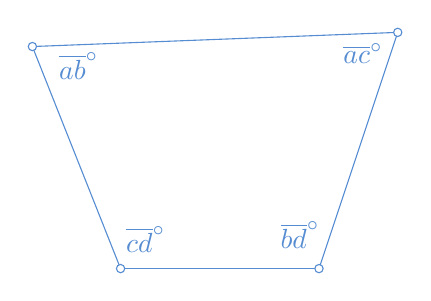
\begin{tikzpicture}[cackithi, node font= /small]
			\draw  (5.48,-1.)-- (8.,-1.);
			\draw  (8.,-1.)-- (9.,2.);
			\draw  (9.,2.)-- (4.36,1.82);
			\draw  (4.36,1.82)-- (5.48,-1.);
			\draw [fill=white] (5.48,-1.) circle (1.5pt);
			\draw (5.8,-0.63) node {$\overline{cd}^\circ$};
			\draw [fill=white] (8.,-1.) circle (1.5pt);
			\draw (7.76,-0.57) node {$\overline{bd}^\circ$};
			\draw [fill=white] (9.,2.) circle (1.5pt);
			\draw (8.56,1.73) node {$\overline{ac}^\circ$};
			\draw [fill=white] (4.36,1.82) circle (1.5pt);
			\draw (4.95,1.57) node {$\overline{ab}^\circ$};
		\end{tikzpicture}
		\vspace*{-10pt}
	\end{figure}
	\textit{Lời giải.} Do tổng bốn góc trong từ giác bằng $360^\circ,$ ta có
	\begin{align*}
		&10a + b + 10a + c + 10b + d + 10c + d \\
		= \,&20a+ 11b+11c+2d=360. \tag{$1$}
	\end{align*}
	Nhận xét rằng nếu $a\le 7$ thì  tổng trong $(1)$ không vượt quá $20\times 7 + 11\times 9 +11\times 9 + 2\times 9 =356.$ Do đó $a$ chỉ có thể nhận giá trị $8$ hoặc $9.$
	Do $b$ và $c$ có thể đổi vai trò cho nhau mà đáp án không thay đổi, ta có thể giả sử $b\ge c.$
	\vskip 0.1cm
	Trường hợp $I$: $a=8.$ Vì trong bốn góc phải có một góc không bé hơn $90^\circ$ nên $b=9.$ Phương trình $(1)$ trở thành $11c+2d=101$ và chỉ có nghiệm duy nhất là $c=9, d=1.$   
	\vskip 0.1cm
	Trường hợp $II$ $a=9$. Nếu $b\le 7$ thì tổng trong ($1$) không vượt quá $20\times 9 + 11\times 7 +11\times 7 + 2\times 9 = 352 < 360$ vô lý. Vậy $b = 8$ hoặc $b = 9$.
	\vskip 0.1cm
	Trường hợp $IIa$: $b=8.$ Phương trình $(1)$ trở thành $11c+2d=92.$ Do $c\le b=8,$ nên ta chỉ có nghiệm duy nhất $c=8, d=2.$
	\vskip 0.1cm
	Trường hợp $IIb$: $b=9.$ Phương trình $(1)$ trở thành $11c+2d=81.$ Dễ thấy phương trình chỉ có nghiệm duy nhất $c=7, d=2.$
	\vskip 0.1cm
	Tóm lại, có ba bộ bốn góc thỏa mãn bài toán: $\{\!89,\! 89,\! 91,\! 91\!\}\!,\! \{\!98,\! 98,\! 82,\! 82\!\}\!,\! \{\!99,\! 97,\! 92,\! 72\!\}.$
	\vskip 0.1cm
	{\bf\color{cackithi}OC$\pmb{32.}$} Cho hình ngũ giác đều $ABCDE$. Vẽ hai đường tròn: một có
	tâm $A$ và bán kính $AB$, và hình kia có tâm $B$ và bán kính $BA$. Gọi $X$ là giao điểm bên trong ngũ giác của hai đường tròn.
	Hỏi số đo của $\angle DEX$ bằng bao nhiêu?
	\vskip 0.1cm
	\textit{Lời giải.} Do $AX, BX, AB$ đều là bán kính của hai đường tròn nên chúng bằng nhau. Như vậy $ABX$ là tam giác đều. Vì mỗi góc trong ngũ giác đều  bằng $\frac{540^\circ}{5}=108^\circ,$ ta có $\angle EAX = 108^\circ - 60^\circ = 48^\circ.$
	\begin{figure}[H]
		\vspace*{-5pt}
		\centering
		\captionsetup{labelformat= empty, justification=centering}
		\definecolor{qqwuqq}{rgb}{0.,0.39215686274509803,0.}
		\definecolor{uuuuuu}{rgb}{0.26666666666666666,0.26666666666666666,0.26666666666666666}
		\definecolor{xdxdff}{rgb}{0.49019607843137253,0.49019607843137253,1.}
		\begin{tikzpicture}[cackithi,scale=1.2]
			\draw [shift={(1.3819660112501053,1.9021130325903073)},,color=qqwuqq,fill=qqwuqq,fill opacity=0.10000000149011612] (0,0) -- (-6.:0.6) arc (-6.:36.:0.6) -- cycle;
			\draw [] (2.,0.)-- (4.,0.);
			\draw [] (4.,0.)-- (4.618033988749895,1.9021130325903064);
			\draw [] (4.618033988749895,1.9021130325903064)-- (3.,3.077683537175253);
			\draw [] (3.,3.077683537175253)-- (1.3819660112501053,1.9021130325903073);
			\draw [] (1.3819660112501053,1.9021130325903073)-- (2.,0.);
			\draw [] (1.3819660112501053,1.9021130325903073)-- (3.,1.7320508075688772);
			\draw [] (3.,1.7320508075688772)-- (2.,0.);
			\draw [] (4.,0.)-- (3.,1.7320508075688772);
			\draw [shift={(4.,0.)},]  plot[domain=0.9272952180016115:3.4474715249946457,variable=\t]({1.*2.*cos(\t r)+0.*2.*sin(\t r)},{0.*2.*cos(\t r)+1.*2.*sin(\t r)});
			\draw [shift={(2.,0.)},]  plot[domain=-0.2992463156024767:2.2003262887940225,variable=\t]({1.*2.*cos(\t r)+0.*2.*sin(\t r)},{0.*2.*cos(\t r)+1.*2.*sin(\t r)});
			
				\draw [fill=white] (2.,0.) circle (1.5pt);
				\draw[] (1.7,-0.09) node {$A$};
				\draw [fill=white] (4.,0.) circle (1.5pt);
				\draw[] (4.3,-0.15) node {$B$};
				\draw [fill=white] (4.618033988749895,1.9021130325903064) circle (1.5pt);
				\draw[] (4.76,2.27) node {$C$};
				\draw [fill=white] (3.,3.077683537175253) circle (1.5pt);
				\draw[] (3.14,3.45) node {$D$};
				\draw [fill=white] (1.3819660112501053,1.9021130325903073) circle (1.5pt);
				\draw[] (1.2,2.29) node {$E$};
				\draw [fill=white] (3.,1.7320508075688772) circle (1.5pt);
				\draw[] (3.04,2.19) node {$X$};
		\end{tikzpicture}
		\vspace*{-10pt}
	\end{figure}
	Mặt khác, tam giác $AEX$ cân tại $A,$ nên $\angle AEX= \frac{180^\circ-48^\circ}{2}= 66^\circ.$ Ta nhận được $\angle DEX= 108^\circ - 66^\circ= 42^\circ.$
	\vskip 0.1cm
	{\bf\color{cackithi}OC$\pmb{33.}$} Seth làm $n$ viên xúc xắc giống hệt nhau bằng cách gấp $n$ bản giống như trong hình bên. Sau đó, anh ta xếp lần lượt các viên xúc xắc chồng lên nhau thành một hình tháp thẳng đứng.
	Biết rằng tổng số chấm ở mỗi một trong bốn mặt xung quanh của tháp xúc xắc đều là số lẻ. Hỏi các giá trị có thể của $n$ là bao nhiêu?
	\begin{figure}[H]
		\vspace*{-5pt}
		\centering
		\captionsetup{labelformat= empty, justification=centering}
		\hspace*{5pt}\includegraphics[height= 0.8\linewidth]{OC33}
		\includegraphics[height= 0.8\linewidth]{OC}
		\vspace*{-10pt}
	\end{figure}
	\textit{Lời giải.} Giả sử tổng số chấm trên $n$ ô của mặt đằng trước của tháp xúc xắc là $T$ và của mặt đằng sau là $S.$ Do tổng $2$ ô trên $2$ mặt đối diện của mỗi viên xúc xắc bằng $7,$ ta có $T+S=7n.$ Theo đầu bài thì cả $T$ và $S$ đều lẻ nên $n$ phải chẵn.
	\vskip 0.1cm
	Ta sẽ chứng minh rằng với mọi $n$ chẵn ta đều có thể xếp được một tháp xúc xắc như vậy. Trước tiên ta xếp $n$ viên xúc xắc theo hướng giống hệt nhau thành một tháp có mỗi mặt gồm toàn các số giống nhau. Sau đó ta xoay viên xúc xắc ở trên cùng đi sao cho các mặt trước, sau đổi chỗ cho nhau và các  mặt trái, phải cũng đổi chỗ cho nhau. 
	\vskip 0.1cm
	Bên dưới là hình minh họa trong trường hợp $n=4.$   Như vậy, tổng các chấm trên mỗi mặt của tháp có dạng $(n-1)a + 7-a=(n-2)a+7$ luôn là số lẻ. Do đó có thể xếp được tháp xúc xắc khi và chỉ khi $n$ chẵn.  
	\begin{figure}[H]
		\vspace*{-5pt}
		\centering
		\captionsetup{labelformat= empty, justification=centering}
		\includegraphics[width= 0.3\linewidth]{OC33b}
		\vspace*{-10pt}
	\end{figure}
	Trong phần cuối của chuyên mục kỳ này, chúng tôi sẽ giới thiệu với bạn đọc ba bài toán trong kỳ thi Olympic toán học trẻ  của Thổ Nhĩ Kỳ. Các bài toán này phù hợp với trình độ học sinh lớp $8-10$.
	\vskip 0.1cm
	{\bf\color{cackithi}OC$\pmb{40.}$} Cho $x, y, z$ là các số thực dương với $x\le 1.$ Chứng minh rằng
	\begin{align*}
		xy+y+2z \geq 4 \sqrt{xyz}.
	\end{align*}
	{\bf\color{cackithi}OC$\pmb{41.}$} Trong một trường có $101$ học sinh, mỗi học sinh có ít nhất một người bạn thân trong số các học sinh khác trong trường. Chứng minh rằng với mọi số nguyên $n, 1<n<101,$ ta có thể chọn một nhóm $n$ học sinh trong trường này sao cho mỗi học sinh được chọn có ít nhất một bạn thân trong số các học sinh khác được chọn. (Biết rằng nếu  $A$ là bạn thân của $B$ thì $B$ cũng là bạn thân của $A$).
	\vskip 0.1cm
	{\bf\color{cackithi} OC$\pmb{42.}$} Cho $m, n, a, k$ là các số nguyên dương và $k>1$ sao cho đẳng thức sau thỏa mãn 
	\begin{align*}
		5^m+63n+49=a^k.
	\end{align*} Tìm giá trị nhỏ nhất của $k$.
\end{multicols}

%	\newpage
%
%	\setcounter{figure}{0}
%	\thispagestyle{diendandayvahoctoannone}
\pagestyle{diendandayvahoctoan}
\everymath{\color{diendantoanhoc}}
\graphicspath{{../diendantoanhoc/pic/}}
\blfootnote{$^{1}$\color[named]{diendantoanhoc}Tòa soạn Hà Nội, Báo Thanh Niên.}
\begingroup
\AddToShipoutPicture*{\put(0,616){\includegraphics[width=19.3cm]{../bannerdiendan}}}
\AddToShipoutPicture*{\put(56,530){\includegraphics[scale=1]{../tieude.pdf}}}
\centering
\endgroup
\vspace*{182pt}

\textit{\textbf{\color{diendantoanhoc}LTS.} Phan Thành Nam dành giải thưởng của Hội toán học châu Âu năm $2020$. Giải thưởng này được trao bốn năm một lần trong Đại hội Toán học Châu Âu (ECM) cho các nhà khoa học trẻ (không quá $35$ tuổi) nhằm ghi nhận những đóng góp xuất sắc trong lĩnh vực toán học. Nhân dịp Phan Thành Nam về công tác tại Việt Nam, anh đã có những chia sẻ với Pi về con đường học tập của mình.}
\begin{multicols}{2}
	Dù ẵm giải nhì học sinh giỏi văn cấp tỉnh dành cho học sinh THCS nhưng cậu học trò Phan Thành Nam lại ước mơ trở thành nhà vật lý. Vậy là anh quyết tâm thi chuyên toán vì nghe nói muốn hiểu vật lý thì phải giỏi toán. Giấc mơ thưở thiếu thời đó đã dẫn dắt anh đến với giải thưởng chính của Hội toán học châu Âu EMS, bởi những thành tựu dùng toán để giải quyết các vấn đề vật lý lượng tử~...
	\begin{figure}[H]
		\centering
		\vspace*{-5pt}
		\captionsetup{labelformat= empty, justification=centering}
		\includegraphics[width=1\linewidth]{1}
		\caption{\small\textit{\color{diendantoanhoc}GS. Phan Thành Nam tại Viện nghiên cứu cao cấp về Toán. Ảnh: Quang Huy.}}
		\vspace*{-10pt}
	\end{figure}
	\textbf{\color{diendantoanhoc}Ước mơ khởi đầu: trở thành nhà vật lý}
	\vskip 0.1cm
	\textit{Xin chào Phan Thành Nam, anh có thể chia sẻ với Pi về hành trình dẫn anh đến với toán học? Hẳn là anh đã từng là học sinh chuyên toán từ nhỏ, vào ĐH cũng học toán?}
	\vskip 0.1cm
	Đúng là hồi lớp $6$ thì tôi học chuyên toán trường Lương Văn Chánh ở Phú Yên. Gọi là lớp chuyên toán nhưng cũng chỉ khác lớp thường là mỗi tuần chúng tôi được bồi dưỡng thêm vài buổi với nội dung học vượt ra ngoài sách giáo khoa, còn giờ học chính khóa thì cũng học như các bạn lớp thường. Nhưng sau đó mô hình chuyên cấp THCS không còn, lên lớp $7$ tôi trở về học lớp thường. Tôi học đều và thích nhiều môn, năm lớp $9$ còn được giải nhì học sinh giỏi cấp tỉnh môn văn.
	\vskip 0.1cm
	\textit{Ơ, sao tự nhiên anh lại đi thi học sinh giỏi môn văn?}
	\vskip 0.1cm 
	Ban đầu tôi thi học sinh giỏi toán, nhưng bị trượt, không được chọn vào đội tuyển của trường để đi thi tiếp. Vì thế mà cô giáo dạy văn khích lệ tôi thi học sinh giỏi môn văn. Tôi thấy đây là một gợi ý hay, môn văn là môn ``truyền thống" của gia đình tôi, mẹ tôi là giáo viên văn, ba tôi vốn học cử nhân văn ở Trường ĐH Tổng  hợp Huế và sau này làm nhà báo. Trong nhà tôi có rất nhiều sách văn học, lúc rảnh rỗi tôi đọc hết nên cũng rất thích môn văn.  
	\vskip 0.1cm
	\textit{Giải nhì văn cấp tỉnh là một thành tựu ngọt ngào, sao anh không tiếp tục đầu tư cho môn văn mà lại trở thành nhà toán học?}
	\vskip 0.1cm 
	Thật ra khi đó tôi lại ôm ấp một giấc mơ khác, đó là trở thành nhà vật lý. Ấy là do ảnh hưởng của cuốn sách \textbf{\color{diendantoanhoc}\textit{``Các nhà vật lý đi tiên phong"}}, mà hồi đó tôi vừa đọc xong. Tuy nhiên trong sách đó viết rằng để hiểu vật lý thì phải giỏi toán, nên khi vào cấp $3$, tôi chọn thi vào lớp chuyên toán ở Trường THPT chuyên Lương Văn Chánh. 
	\vskip 0.1cm
	\textit{Thi vào đội tuyển toán của trường THCS mà còn bị trượt, vậy mà lại tiếp tục mơ mộng thi vào chuyên toán trường chuyên của tỉnh. Xem ra anh cũng ``liều"?} 
	\vskip 0.1cm
	Đúng là có một chút liều. Nhưng vì nhờ việc trượt đội tuyển toán ở lớp $9$ mà tôi nhận ra mình còn thiếu kiến thức nào để bổ sung trong quá trình ôn thi vào lớp $10$ chuyên toán sau này. Trước đó tôi gần như không học nội dung gì ngoài SGK. Khi ôn thi chuyên toán, tôi mới bắt đầu đào sâu một số nội dung ngoài SGK.
	\vskip 0.1cm
	Thật may là tôi đã đỗ chuyên toán, tuy với mức điểm trung bình nhưng đó là một sự khởi đầu tuyệt vời bởi từ đó tôi được học các thầy dạy toán rất giỏi, họ gieo vào tôi tình yêu, niềm đam mê với toán. 
	\vskip 0.1cm
	\textbf{\color{diendantoanhoc}Học để thỏa mãn đam mê chứ không vì thi thố}
	\vskip 0.1cm
	\textit{Đỗ chuyên toán với mức điểm trung bình, vậy việc học sau đó của anh có chật vật để theo kịp các bạn trong lớp không?}
	\vskip 0.1cm
	Tôi thấy việc học cũng nhẹ nhàng. Cuối năm lớp $10$ tôi còn được chọn đi dự kỳ thi Olympic $30.4$, nhờ đó mà tôi được giao lưu với các bạn học sinh giỏi toán các địa phương khác. Chúng ta vẫn nói về tầm quan trọng của việc được học với các thầy giỏi, nhưng từ trải nghiệm của chính mình, tôi thấy việc được học chung với các bạn giỏi cũng quan trọng không kém. 
	\vskip 0.1cm
	Hồi đó lớp tôi có một bạn rất giỏi, tên là Phùng Trọng Thực (hiện là GV Trường ĐH Bách khoa TP.HCM). Có lần Thực đưa cho tôi một bài toán rất hay và lạ, hỏi có giải được không? Thực cho biết bài toán đó có trong tờ tạp chí Toán học và Tuổi trẻ, đây là lần đầu tôi biết tới tạp chí này. Từ đó, $2$ đứa cùng có thêm một niềm vui chung là ngóng chờ tạp chí \textbf{\color{diendantoanhoc}\textit{Toán học và Tuổi trẻ}} về hàng tháng để ngồi giải bài. Chúng tôi áng chừng thời gian tạp chí về đến Phú Yên (thường chậm hơn thời điểm phát hành ở Hà Nội vài ngày), những ngày đó lảng vảng quanh bưu điện liên tục để hễ tạp chí về đến nơi là mua được ngay. 
	\vskip 0.1cm
	Thời gian đầu, gần như chúng tôi chẳng giải được bài toán nào đăng trong tạp chí đó. Lúc đó chúng tôi mới vào lớp $10$, nhưng có nhiều bài thuộc chương trình lớp $11-12$, nên chúng tôi tự học các kiến thức liên quan trong SGK các lớp trên để có đủ nền tảng cần thiết. Nhờ sự ``máu mê" đó mà chúng tôi bắt đầu giải được bài đầu tiên, rồi bài thứ  hai, thứ ba ...
	\vskip 0.1cm 
	Lên lớp $11$ thì tôi đạt giải nhì HSG quốc gia, được ra Hà Nội thi chọn đội tuyển quốc tế. Có khoảng $40$ bạn dự thi, để chọn ra $6$ bạn. Đề thi rất khó, có những dạng toán tôi chưa gặp bao giờ. Tôi nhớ một kỷ niệm vui là nhờ được mang đồ ăn vào phòng thi, mà tôi có việc để làm lúc thi, tức là tôi chủ yếu ngồi ăn chứ toán thì không làm được bao nhiêu.  
	\vskip 0.1cm
	Lớp $12$ tôi cũng được đi thi quốc gia, nhưng chỉ đạt giải khuyến khích. Lúc đó tôi cảm thấy rất tự tin, vì đã học thêm được rất nhiều kiến thức so với năm lớp $11$, nhưng khi vào phòng thi lại làm bài không tốt.  
	\vskip 0.1cm
	\textit{Không được ``hái quả ngọt" vào năm học lớp $12$ mà anh không nản lòng à, để lại vẫn tiếp tục học toán khi lên ĐH?}   
	\vskip 0.1cm
	Lúc đó tình yêu toán đã bén rễ sâu đậm trong tôi, tôi học là để thỏa mãn đam mê chứ không phải để thi thố. 
	\vskip 0.1cm
	Nhờ đạt giải học sinh giỏi quốc gia, tôi được tuyển thẳng vào ĐH. Lúc đó tôi có nhiều lựa chọn. Ngành CNTT của Trường ĐH Bách khoa TP.HCM là ngành thời thượng. Các trường y dược cũng là mục tiêu phấn đấu của nhiều bạn học sinh giỏi. Còn khoa toán tin Trường ĐH Khoa học tự nhiên, ĐH Quốc gia TP.HCM có điểm chuẩn rất thấp, khoảng $15$ điểm/$3$ môn là đỗ. Tuy nhiên tôi chẳng bận tâm, vì thích toán quá rồi, cứ được học toán tiếp là tôi học. 
	\vskip 0.1cm
	Lúc đó tôi rất thích cuốn sách \textbf{\color{diendantoanhoc}\textit{``Tìm tòi để học giỏi toán"}} của anh Lê Quang Nẫm. Biết anh Nẫm là sinh viên Trường ĐH Khoa học tự nhiên, ĐH Quốc gia TP.HCM, tôi muốn vào đó học, với hy vọng có cơ hội được gặp anh, hoặc được học với các thầy của anh. 
	\vskip 0.1cm
	Anh Lê Quang Nẫm hơn tôi khoảng $5$ tuổi, lúc là học sinh đã rất nổi tiếng. Anh là con nhà nghèo, khi anh trúng tuyển vào lớp $10$ Trường Phổ thông Năng khiếu của ĐH Quốc gia TP.HCM thì ba của anh phải từ Quảng Ngãi vào TP.HCM để đạp xích lô nuôi anh ăn học. Học xong cấp $3$ anh vào khoa Toán tin Trường ĐH Khoa học tự nhiên, và tốt nghiệp thủ khoa. Nhưng đó là những thông tin về sau tôi mới biết. Còn khi đọc cuốn sách của anh Nẫm tôi cảm thấy ngưỡng mộ vì anh viết hấp dẫn quá. 
	\vskip 0.1cm
	\textit{Ba mẹ anh có ý kiến thế nào khi anh chọn học toán?}
	\vskip 0.1cm 
	Ba mẹ tôi dân chủ lắm, chỉ cung cấp thông tin về một số trường/ngành mà ba mẹ nghĩ là tốt, còn quyết định là do tôi. Thật sự lúc đó tôi cũng không mường tượng con đường học Toán ở ĐHKHTN TPHCM là như thế nào. Tôi chỉ nghĩ là có thể nó sẽ giúp mình trở thành giáo viên dạy toán, mà như thế cũng tốt. Thời đó sinh viên tốt nghiệp các ngành khoa học cơ bản mà có chứng chỉ sư phạm là cũng được dạy phổ thông. 
	\vskip 0.1cm
	Đó là một quyết định sáng suốt. Vì khi vào học đại học thì tôi rất may mắn gặp được các thầy giỏi, tâm huyết. Thầy này giúp tôi đến với thầy khác, nhờ thế mà hành trình giúp tôi đến với toán học khá suôn sẻ. 
	\vskip 0.1cm
	\textbf{\color{diendantoanhoc}Dùng toán để hiểu vật lý và khám phá thế giới}
	\vskip 0.1cm 
	\textit{Anh được Hội toán học châu Âu trao giải thưởng chính là bởi thành tựu nào trong nghiên cứu toán học của anh?}
	\vskip 0.1cm 
	Họ xét giải trên cơ sở một cụm công trình, cụ thể là ghi nhận đóng góp của tôi cho lĩnh vực vật lý lượng tử đa hạt. Thông thường trong vật lý lượng tử, để biết tính chất của một hệ thì mình phải giải một phương trình Schrödinger (phương trình đươc đặt theo tên nhà vật lý học người Áo, người đầu tiên thiết lập phương trình này và được giải Nobel vật lý năm $1933$). Nếu hệ chỉ có một hạt, thì phương trình Schrödinger chỉ có một biến trong không gian ba chiều. Nếu hệ có $N$ hạt thì phương trình có $N$ biến, và trong nhiều ứng dụng số lượng biến số rất lớn tới mức mình không thể giải được, kể cả giải chính xác hoặc giải số bằng máy tính. 
	\vskip 0.1cm
	%	\begin{figure}[H]
		%		\centering
		%		\vspace*{-5pt}
		%		\captionsetup{labelformat= empty, justification=centering}
		%		\includegraphics[width=1\linewidth]{3}
		%		\caption{\small\textit{\color{diendantoanhoc}GS. Phan Thành Nam và một sinh viên. Anh: Quang Huy.}}
		%		\vspace*{-10pt}
		%	\end{figure}
	Vì đó là một bài toán rất phức tạp, mình cần sẽ tiếp cận bằng các phương pháp xấp xỉ, thường là thay phương trình tuyến tính nhiều biến bằng phương trình phi tuyến một biến. Đây là phương pháp mà các nhà vật lý học đã phát triển trong một thời gian dài. Câu hỏi đặt ra là làm sao chứng minh được phương pháp xấp xỉ đó là đúng, nghĩa là khi số hạt N tiến về vô cùng thì mô hình xấp xỉ trở thành chính xác. Bằng cách sử dụng và phát triển các công cụ trong toán giải tích, tôi chứng minh được rằng trong những điều kiện cụ thể thì một số mô hình xấp xỉ sẽ đúng với những nguyên lý căn bản trong cơ học lượng tử. 
	\vskip 0.1cm
	\textit{Ở trên anh kể chuyện hồi lớp $9$ anh từng mơ ước trở thành nhà vật lý nên nên mới cố gắng học giỏi toán. Vậy việc sau này anh chọn nghiên cứu sâu về toán trong vật lý lượng tử, việc này có liên quan gì tới ước mơ hồi đó?}
	\vskip 0.1cm 
	Đúng là có liên quan. Sau khi làm thạc sĩ, tôi xin được một số học bổng tiến sĩ khác nhau, có cả toán lý thuyết và toán ứng dụng. Tình cờ trong thời gian này, tôi đọc một cuốn sách rất thú vị là \textbf{\color{diendantoanhoc}\textit{``Lưới trời ai dệt"}} của tác giả Nguyễn Tường Bách. Trong cuốn đó, tác giả trình bày về vật lý lượng tử một cách rất cuốn hút, với nhiều mối liên quan tới triết học Phật giáo. Điều này làm sống lại uớc mơ hồi năm lớp $9$, vốn vẫn quanh quẩn trong tâm trí tôi, đó là học về Vật lý Toán.  
	\vskip 0.1cm
	Vì thế mà tôi chọn GS Jan Philip Solovej ở ĐH Copenhaghen để xin học lên tiến sĩ. Khi đó, tôi vào trang khoa toán tìm các giáo sư, và cảm thấy các công trình nghiên cứu của GS Solovej về vật lý lượng tử là vô cùng hấp dẫn. Mặc dù tôi không hiểu rõ các công trình đó, nhưng cảm thấy các kiến thức toán này nếu cố gắng mình sẽ học được, nên quyết định xin theo thầy. Tôi rất may mắn là được thầy đồng ý. 
	\vskip 0.1cm
	Tôi nghĩ môn vật lý ở chương trình phổ thông là một môn học thú vị, nó giúp cho những đứa trẻ thỏa mãn sự tò mò khi tìm hiểu các hiện tượng tự nhiên. Sau này, nhờ sử dụng các công cụ bên toán mà tôi hiểu được chính xác các khái niệm vật lý, điều này kiến tôi thấy rất sung sướng. Mặc dù có thể đó là những điều nhân loại hiểu ra từ cách đây hàng trăm năm, nhưng khi được đi lại trên con đường khám phá thế giới mà nhân loại đã từng đi, tôi vẫn thấy thật hạnh phúc. 
	\vskip 0.1cm
	\textbf{\color{diendantoanhoc}Sẽ cùng các đồng nghiệp người Việt ở nước ngoài giúp VN lấp khoảng trống vật lý toán...}
	\vskip 0.1cm
	\textit{Anh có biết, ở Việt Nam, có những ai làm việc trong lĩnh vực nghiên cứu của anh không?}
	\vskip 0.1cm 
	Tôi gần như không biết có ai làm về lĩnh vực này ở VN! Có một số nhóm vật lý lý thuyết làm việc trực tiếp với những mô hình xấp xỉ phi tuyến, và một số nhóm vật lý thực nghiệm kiểm tra các mô hình xấp xỉ đó có đúng hay không. Nhưng có vẻ như không có nhà toán học nào nghiên cứu những phương trình nhiều hạt từ các nguyên lý cơ \linebreak bản nhất.  
	\vskip 0.1cm
	\textit{Có nghĩa là lĩnh vực này đang có một khoảng trống lớn ở VN?}
	\vskip 0.1cm 
	Vâng, đúng rồi. Nhưng tôi nghĩ tôi có thời gian để giúp cải thiện việc này. 
	\vskip 0.1cm
	Đầu tháng $8$ vừa rồi, tôi cùng anh Nguyễn Trọng Toán (GS ở ĐH bang Pennsylvania, Mỹ) tổ chức một trường hè về vật lý toán bên Viện Nghiên cứu cao cấp về Toán (nơi GS Ngô Bảo Châu là Giám đốc khoa học -- PV). Chúng tôi bất ngờ trước sự say mê học hỏi của các bạn trẻ. Trong cả buổi sáng họ nghe chúng tôi giảng bài, tới buổi chiều vẫn kiên trì ngồi lại lớp học làm bài tập. Sau đó tôi dự hội thảo về phương trình đạo hàm riêng kỷ niệm ngày sinh GS Đinh Nho Hào ở Viện toán học VN. Tôi thấy nhiều báo cáo đạt chất lượng rất cao, ngang tầm chất lượng các hội thảo đẳng cấp quốc tế. Điều đặc biệt là có nhiều báo cáo của các bạn trẻ. Do đó, tôi thấy rất lạc quan với sự phát triển của ngành này ở trong nước, và trước mắt tôi có thể dùng các công cụ của ngành phương trình đạo hàm riêng để tương tác với các nhà toán học trong nước. 
	\vskip 0.1cm
	%	\begin{figure}[H]
		%		\centering
		%		\vspace*{5pt}
		%		\captionsetup{labelformat= empty, justification=centering}
		%		\includegraphics[width=1\linewidth]{4}
		%		\caption{\small\textit{\color{diendantoanhoc}GS. Phan Thành Nam báo cáo tại Viện Toán học. Ảnh: Viện Toán học.}}
		%		\vspace*{-10pt}
		%	\end{figure}
	Để xây dựng ngành của mình ở VN, tôi cần phải tiếp tục tổ chức một số trường hè, tổ chức dạy học một số môn học trong các khoa toán của các trường ĐH. Tôi đã trao đổi với một số nhà toán học trong nước và được các anh ủng hộ. Trước hết các thầy trong nước sẽ dạy trước cho sinh viên một số kiến thức tổng quát, sau đó tôi sẽ dạy phần tiếp theo, đi sâu hơn vào lĩnh vực nghiên cứu hiện đại. Bằng các giải pháp đồng thời như trên, tôi hy vọng sẽ có một số bạn trẻ sẽ nảy sinh đam mê về vật lý toán.
	\vskip 0.1cm 
	Một thuận lợi là với riêng ngành giải tích -- phương trình đạo hàm riêng, tôi có nhiều ``đồng minh" là các anh chị người Việt xuất thân từ trường ĐH Khoa học tự nhiên, ĐH Quốc gia TP.HCM và đã đạt được vị trí vững vàng trong các trường đại học hàng đầu trên thế giới. Ở Châu Âu có anh Nguyễn Hoài Minh (GS ĐH Paris Sorbonne ở Pháp); anh Nguyễn Lê Lực (GS ĐH ở Anh); anh Trương Trung Tuyến (GS ĐH Oslo, Na Uy). Ở Mỹ có anh  Nguyễn Trọng Toán (GS ĐH bang Pennsylvania), anh Lê Quang Nẫm (GS ĐH Indiana), anh Trần Vĩnh Hưng (GS ĐH Wisconsin–Madison), anh Phan Văn  Tuộc (GS ĐH Tennessee), anh Trần Minh Bình (GS ĐH Texas A\&M) ... và rất nhiều anh chị khác. Đó là những người trẻ trên dưới $40$ tuổi, đang làm việc rất tích cực, và mọi người đều đồng lòng hướng về VN với mong muốn tham gia vào sự phát triển toán học trong nước.
	\vskip 0.1cm
	\textit{Xin cảm ơn GS Phan Thành Nam!} 
\end{multicols}
%	\newpage
%
%	\setcounter{figure}{0}
%	\thispagestyle{doisongtoanhocnone}
\pagestyle{doisongtoanhoc}
\everymath{\color{doisongtoanhoc}}
\graphicspath{{../doisongtoanhoc/pic/}}
\blfootnote{$^1$\color{doisongtoanhoc}Trung tâm Thông tin -- Tư liệu, Viện Hàn lâm Khoa học và Công nghệ Việt Nam.}
\begingroup
\AddToShipoutPicture*{\put(0,616){\includegraphics[width=19.3cm]{../bannerdoisong}}}
\AddToShipoutPicture*{\put(80,475){\includegraphics[scale=0.95]{../tieude.pdf}}}\centering
\endgroup

\vspace*{230pt}


\begin{multicols}{2}	
	Ngày $25/3/2023$, tại Hà Nội, Viện Toán học, Trung tâm Thông tin -- Tư liệu, Viện Hàn lâm Khoa học và Công nghệ Việt Nam và Trung tâm Quốc tế Đào tạo và Nghiên cứu Toán học (trực thuộc Viện Toán học, được UNESCO bảo trợ) đã đồng tổ chức ngày ``Toán học dành cho mọi người". Đây là hoạt động hưởng ứng Ngày Toán học Thế giới năm $2023$, đã thu hút đông đảo các nhà khoa học, giáo viên, sinh viên và học sinh trên cả nước tham dự.
	\vskip 0.1cm
	GS. Hoàng Tụy ($1927 - 2019$) là một nhà Toán học xuất sắc, đồng thời cũng là một nhà sư phạm mẫu mực. Trước khi biên soạn những giáo trình đại học được nhiều thế hệ sinh viên, nghiên cứu sinh sử dụng, GS. Hoàng Tụy từng biên soạn những bài giảng đầu tiên cho hệ thống giáo dục quốc dân. Cả cuộc đời cống hiến cho Toán học, Ông không ngừng trăn trở về nền giáo dục nước nhà. Được sự đồng ý của gia đình GS. Hoàng Tụy, Kỳ thi ``Bài giảng và bài viết về Toán học, mang tên Hoàng Tụy" được tổ chức với sự phối hợp của Tạp chí Pi và Trung tâm Quốc tế Đào tạo và Nghiên cứu Toán học.
	\vskip 0.1cm
	Với mục tiêu khích lệ sự tìm tòi, sáng tạo của giáo viên, sinh viên và mọi người yêu Toán học trong việc giảng dạy, đồng thời quảng bá Toán học, khơi dậy lòng say mê Toán học trong học sinh và công chúng, Kỳ thi ``Bài giảng và bài viết mang tên Hoàng Tụy" đã thu hút nhiều tác giả gửi hồ sơ tham gia. 
	\vskip 0.1cm
	Chủ đề của Kỳ thi lần thứ hai, năm $2023$ là: Tìm hiểu về môn Toán trong 	``Chương trình giáo dục phổ thông mới" thông qua một chủ đề cụ thể; Tìm hiểu về Toán sơ cấp, Lịch sử Toán học và Toán học trong cuộc sống. Hội đồng giám khảo năm nay gồm: 
	\vskip 0.1cm
	--	GS.TSKH. Ngô Việt Trung (Chủ tịch Hội Toán học Việt Nam, Nguyên Viện trưởng Viện Toán học), Chủ tịch Hội đồng;
	\vskip 0.1cm 
	--	GS.TSKH. Đỗ Đức Thái (Đại học Sư phạm Hà Nội, Phó Chủ tịch Hội Toán học Việt Nam);
	\vskip 0.1cm
	--	GS.TSKH. Phùng Hồ Hải (Phó Chủ tịch Hội Toán học Việt Nam, Nguyên Viện trưởng Viện Toán học);
	\vskip 0.1cm
	--	GS.TSKH. Hà Huy Khoái (Viện trưởng viện Toán học và khoa học ứng dụng Trường Đại học Thăng Long, Nguyên Viện trưởng Viện Toán học);
	\vskip 0.1cm
	--	TS. Trần Nam Dũng (Phó Hiệu trưởng Trường Phổ thông Năng khiếu, Đại học Quốc gia Thành phố Hồ Chí Minh);
	\vskip 0.1cm
	--	PGS. TS Phó Đức Tài (Trưởng khoa Toán--Cơ--Tin học, Trường Đại học Khoa học Tự Nhiên, Đại học Quốc gia Hà Nội).
	\begin{figure}[H]
		\vspace*{-5pt}
		\centering
		\captionsetup{labelformat= empty, justification=centering}
		\includegraphics[width= 1\linewidth]{1}
		\caption{\small\textit{\color{doisongtoanhoc}Giáo sư Ngô Việt Trung, Chủ tịch Hội Toán học Việt Nam, Chủ tịch Hội đồng Giám khảo.}}
		\vspace*{-10pt}
	\end{figure}
	Ban Tổ chức đã tiến hành chấm các hồ sơ dự thi ở vòng sơ khảo, lựa chọn được $8$ hồ sơ tốt nhất để tranh tài tại vòng chung khảo, bao gồm: 
	\vskip 0.1cm
	$1$. Hình có trục đối xứng, tác giả Nguyễn Thụy Việt Anh, Trường Liên cấp Hội nhập Quốc tế Ischool, Quảng Trị; 
	\begin{figure}[H]
		\vspace*{-5pt}
		\centering
		\captionsetup{labelformat= empty, justification=centering}
		\includegraphics[width= 1\linewidth]{2}
%		\caption{\small\textit{\color{}}}
		\vspace*{-10pt}
	\end{figure}
	$2$. Lý thuyết đồ thị và các cấu trúc đáng chú ý, tác giả Hà Trung, Trường THPT chuyên Lê Hồng Phong, Nam Định; 
	\begin{figure}[H]
		\vspace*{5pt}
		\centering
		\captionsetup{labelformat= empty, justification=centering}
		\includegraphics[width= 1\linewidth]{3}
%		\caption{\small\textit{\color{}}}
		\vspace*{-15pt}
	\end{figure}
	$3$. Bổ đề hai đoạn thẳng và một số ứng dụng, tác giả Nguyễn Hữu Tâm, Trường THPT chuyên Lê Quý Đôn, Bình Định; 
	\begin{figure}[H]
		\vspace*{-5pt}
		\centering
		\captionsetup{labelformat= empty, justification=centering}
		\includegraphics[width= 1\linewidth]{4}
%		\caption{\small\textit{\color{}}}
		\vspace*{-15pt}
	\end{figure}
	$4$. Nét đẹp của phương pháp đếm dưới góc nhìn của số Fibonacci, tác giả Nguyễn Tuấn Anh, Trường PTTH chuyên Nguyễn Quang Diêu, Đồng Tháp; 
	\begin{figure}[H]
		\vspace*{-5pt}
		\centering
		\captionsetup{labelformat= empty, justification=centering}
		\includegraphics[width= 1\linewidth]{5}
%		\caption{\small\textit{\color{}}}
		\vspace*{-15pt}
	\end{figure}
	$5$. Một cách thiết kế dạy học Toán theo hướng gắn liền với thực tiễn, tác giả Phạm Đức Quang, Trường Đại học Hà Nội $2$; 
	\begin{figure}[H]
		\vspace*{5pt}
		\centering
		\captionsetup{labelformat= empty, justification=centering}
		\includegraphics[width= 1\linewidth]{6}
%		\caption{\small\textit{\color{}}}
		\vspace*{-15pt}
	\end{figure}
	$6$. Tích hợp tư duy công dân số trong bài giảng môn Toán, tác giả Nguyễn Thế Minh, Trường Trung học Vinschool Imperia, Hải Phòng; 
	\begin{figure}[H]
		\vspace*{-5pt}
		\centering
		\captionsetup{labelformat= empty, justification=centering}
		\includegraphics[width= 1\linewidth]{7}
%		\caption{\small\textit{\color{}}}
		\vspace*{-15pt}
	\end{figure}
	$7$. Mập mờ công thức Euler, tác giả Nguyễn Quang Minh, Biên Hoà, Đồng Nai; 
	\begin{figure}[H]
		\vspace*{-5pt}
		\centering
		\captionsetup{labelformat= empty, justification=centering}
		\includegraphics[width= 1\linewidth]{8}
%		\caption{\small\textit{\color{}}}
		\vspace*{-15pt}
	\end{figure}
	$8$. Giải bài toán tập hợp bằng phương pháp ``ô ăn quan", nhóm tác giả Ngô Quốc Trung, Nguyễn Thị Hiền, Trường Liên cấp Hermann Gmeiner Vinh, Nghệ An. 
	\begin{figure}[H]
		\vspace*{-5pt}
		\centering
		\captionsetup{labelformat= empty, justification=centering}
		\includegraphics[width= 1\linewidth]{9}
%		\caption{\small\textit{\color{}}}
		\vspace*{-15pt}
	\end{figure}
	Trong khuôn khổ Ngày ``Toán học dành cho mọi người", $8$ nhóm tác giả/tác giả đã thuyết trình các bài giảng và bài viết trước Hội đồng giám khảo. Sau những nhận xét công tâm và đánh giá kỹ lưỡng, Ban Tổ chức đã quyết định trao giải cho các tác giả.
	\vskip 0.1cm
	Về chủ đề ``Tìm hiểu về môn Toán trong ``Chương trình giáo dục phổ thông mới" thông qua một chủ đề cụ thể": Không có giải Nhất, giải Nhì được trao cho bài giảng ``Giải bài toán tập hợp bằng phương pháp ô ăn quan", nhóm tác giả Ngô Quốc Trung, Nguyễn Thị Hiền. Bài viết ``Một cách thiết kế dạy học Toán theo hướng gắn liền với thực tiễn", tác giả Phạm Đức Quang đạt giải Ba. Bài giảng ``Tích hợp tư duy công dân số trong bài giảng môn Toán", tác giả Nguyễn Thế Minh và ``Hình có trục đối xứng", tác giả Nguyễn Thụy Việt Anh đạt giải Khuyến khích. 
	\vskip 0.1cm
	Về các chuyên đề khác, giải Nhất được trao cho bài giảng ``Bổ đề hai đoạn thẳng và một số ứng dụng", tác giả Nguyễn Hữu Tâm. Bài giảng ``Mập mờ công thức Euler", tác giả Nguyễn Quang Minh đạt giải Nhì; ``Lý thuyết đồ thị và một số cấu trúc đáng chú ý", tác giả Hà Trung đạt giải Ba; ``Nét đẹp của phương pháp đếm dưới góc nhìn của số Fibonacci", tác giả Nguyễn Tuấn Anh đạt giải Khuyến khích. 
	\end{multicols}
	\begin{figure}[H]
		\vspace*{5pt}
		\centering
		\captionsetup{labelformat= empty, justification=centering}
		\includegraphics[width= 1\linewidth]{10}
		\caption{\small\textit{\color{doisongtoanhoc}Đại diện ban giám khảo và đại diện gia đình GS Hoàng Tụy trao giải cho các tác giả.}}
		\vspace*{-10pt}
	\end{figure}
	\begin{multicols}{2}
	Theo đánh giá của Ban Tổ chức, chất lượng hồ sơ dự thi của các tác giả tại Kỳ thi ``Bài giảng và bài viết về Toán học, mang tên Hoàng Tụy" lần thứ hai, năm $2023$ cao hơn lần thứ nhất, năm $2021$. Điều đó cho thấy Kỳ thi ``Bài giảng và bài viết về Toán học, mang tên Hoàng Tụy" đã được lan tỏa và hưởng ứng mạnh mẽ, trở thành một nhân tố tích cực góp phần nâng cao chất lượng dạy và học Toán ở cấp trung học phổ thông. 
\end{multicols}
\vspace*{-10pt}
{\color{doisongtoanhoc}\rule{1\linewidth}{0.1pt}}
\vskip 0.2cm
{\centerline{\LARGE\textbf{\color{doisongtoanhoc}LỜI GIẢI, ĐÁP ÁN}}}
\begin{multicols}{2}
	\textbf{\color{doisongtoanhoc}Một chuyến thăm triển lãm}
	\vskip 0.1cm
	Người của công ty Tae Yeon không thể trả lời ``Không có ai cả" vì như vậy người đó sẽ nói dối. Vì vậy, người đầu tiên đến từ công ty TeaYon.
	\vskip 0.1cm
	Hai người tiếp theo trả lời giống nhau, vì thế họ phải cùng nói thật hoặc cùng nói dối, tức là đến từ cùng một công ty.
	\vskip 0.1cm
	Nếu cả hai người này cùng đến từ công ty Tae Yeon, suy ra số người của công ty Tae Yeon trong số họ không ít hơn $2$ người. Suy ra câu trả lời của họ là sai. Vì vậy cả hai người thứ hai và thứ ba đều nói dối, tức là đến từ công ty TeaYon.
	\vskip 0.1cm
	Do vậy, trong số $5$ người này, có ít nhất $3$ người của công ty TeaYon và không quá $2$ người đến từ công ty Tae Yeon.
	\vskip 0.1cm
	Nhưng vì cả $3$ người đầu tiên đều nói dối, suy ra số người của công ty Tae Yeon trong số họ không thể là $0$ hoặc $1$. Vì vậy, cả hai người còn lại đều là nhân viên của công ty Tae Yeon. Và họ đều sẽ trả lời là ``Có hai người".
	\vskip 0.1cm
	\textbf{\color{doisongtoanhoc}Đố vui}
	\vskip 0.1cm
	Sau đây là một cách điền thỏa mãn yêu cầu:
	\begin{table}[H]
		\vspace*{-5pt}
		\centering
		\captionsetup{labelformat= empty, justification=centering}
		\setlength{\tabcolsep}{8pt}
		\renewcommand{\arraystretch}{1.2}
		\begin{tabular}{|c|c|c|c|c|c|}
			\hline
			$1$&$4$&$2$&$8$&$5$&$7$\\
			\hline
			$4$&$2$&$8$&$5$&$7$&$1$\\
			\hline
			$2$&$8$&$5$&$7$&$1$&$4$\\
			\hline
			$8$&$5$&$7$&$1$&$4$&$2$\\
			\hline
			$5$&$7$&$1$&$4$&$2$&$8$\\
			\hline
			$7$&$1$&$4$&$2$&$8$&$5$\\
			\hline
		\end{tabular}
		\vspace*{-10pt}
	\end{table}
	\textbf{\color{doisongtoanhoc}Góc cờ}
	\vskip 0.1cm
	$\pmb{1}$\textbf{\color{doisongtoanhoc}.Ha$\pmb{2+}$ Vg}$\pmb{1}$ Nếu $1$...Vh$1$ $2$.Vf$3$ Th$4$ $3$.Hd$2+–$
	\vskip 0.1cm
	$\pmb{2}$\textbf{\color{doisongtoanhoc}.Vf$\pmb{3}$ Th$\pmb{4}$ $\pmb{3}$.He$\pmb{2}$!} Phương án khác cũng dẫn đến Trắng thắng như sau $3$.Hd$2$! Vh$1$ $4$.Hb$2$! Vg$1$ $5$.Hd$4+$ Vh$1$ $6$.Hxh$4$
	\vskip 0.1cm
	$\pmb{3}$\textbf{\color{doisongtoanhoc}...Vh$\pmb{1}$ $\pmb{4}$.Hb$\pmb{2}$! Vg$\pmb{1}$ $\pmb{5}$.Hd}$\pmb{4+}$ Trắng thắng.
\end{multicols}

%	\newpage
%%
%	\setcounter{figure}{0}
%	\thispagestyle{timhieukhoahocnone}
\pagestyle{timhieukhoahoc}
\everymath{\color{timhieukhoahoc}}
\blfootnote{$^1$\text{\color{timhieukhoahoc}Hà Nội.}}
\graphicspath{{../timhieukhoahoc/pic/}}
\begingroup
\AddToShipoutPicture*{\put(0,616){\includegraphics[width=19.3cm]{../bannertimhieu}}}
\AddToShipoutPicture*{\put(76,555){\includegraphics[scale=1]{../tieude.pdf}}}
\centering
\endgroup
\vspace*{155pt}

\begin{multicols}{2}
	Khối lượng của Trái Đất bằng bao nhiêu? Đây là một câu hỏi mà đến thế kỷ $18$ người ta mới có được những kết quả đo đạc tương đối chính xác dựa trên những lý thuyết vật lý được phát triển suốt hai thế kỷ bắt đầu từ những thí nghiệm của Galileo.
	\vskip 0.1cm
	$\pmb{1.}$ \textbf{\color{timhieukhoahoc}Từ Galileo đến Newton}
	\begin{figure}[H]
		\vspace*{-5pt}
		\centering
		\captionsetup{labelformat= empty, justification=centering}
		\includegraphics[width= 0.75\linewidth]{1}
		\caption{\small\textit{\color{timhieukhoahoc}Hình ${1.}$ Galileo và dao động của ngọn đèn trên trần nhà thờ.}}
		\vspace*{-10pt}
	\end{figure}
	Một câu chuyện khá thú vị thường được kể về Galileo và trọng lực là khi ông quan sát ngọn đèn trên trần nhà trong nhà thờ Pisa. Ông dùng mạch đập của mình để tính thời gian của mỗi chu kỳ dao động của nó và nhận thẩy rằng với những góc dao động nhỏ, chu kỳ giao động không thay đổi. Với những thí nghiệm sau này về con lắc đơn, Galileo còn nhận thấy rằng chu kỳ dao động thay đổi theo chiều dài của dây treo (dây treo càng dài thì chu kỳ càng lớn) nhưng lại không phụ thuộc vào khối lượng của con lắc.
	\begin{figure}[H]
		\vspace*{-5pt}
		\centering
		\captionsetup{labelformat= empty, justification=centering}
		\includegraphics[width= 1\linewidth]{2}
		\caption{\small\textit{\color{timhieukhoahoc}Hình $2$. Galileo biểu diễn thí nghiệm về chuyển động trên mặt phẳng nghiêng cho các quý tộc nhà Medici (tranh của Giuseppe  Bezzuoli).}}
		\vspace*{-10pt}
	\end{figure}
	Ông tiếp tục nghiên cứu vấn đề này bằng cách làm thí nghiệm với chuyển động trên mặt phẳng nghiêng, một dạng chuyển động mà ông cho rằng có thể dùng để liên hệ với chuyển động theo cung tròn của con lắc. Thời gian được Galileo đo bằng một đồng hồ nước. Khi hòn bi được thả từ vị trí đầu của mặt phẳng nghiêng thì khóa cũng được mở để nước từ đồng hồ chảy vào một bình chứa bên dưới. Khi hòn bi đến vị trí bị chặn lại thì khóa cũng được đóng lại cùng lúc. Việc đo khối lượng nước trong bình sẽ cho độ dài thời gian của chuyển động. Kết quả thí nghiệm cho thấy quãng đường chuyển động tỷ lệ thuận với bình phương của thời gian. Đồng thời, thời gian chuyển động cho cùng một quãng đường sẽ càng ngắn khi góc nghiêng tăng lên.
	\vskip 0.1cm
	Galileo còn phát hiện ra rằng khi cho hòn bi lăn trên một dây cung có điểm cuối tại vị trí mà đường tròn tiếp xúc phương nằm ngang thì thời gian chuyển động không thay đổi khi ta di chuyển vị trí đầu dây cung trên đường tròn (độc giả có thể thử tự chứng minh bài toán này). Đồng thời, ta cũng có thể coi chuyển động của con lắc đơn dọc theo cung tròn là tổng hợp của nhiều chuyển động trên các đoạn dây cung liên tiếp nhau. Nhận định này cũng là cơ sở giúp Huygens thiết lập phương trình toán học cho chuyển động của con lắc đơn nhiều thập kỷ sau đó.
	\begin{figure}[H]
		\vspace*{-5pt}
		\centering
		\captionsetup{labelformat= empty, justification=centering}
		\includegraphics[height= 0.45\linewidth]{3a}
		\includegraphics[height= 0.45\linewidth]{3b}
		\caption{\small\textit{\color{timhieukhoahoc}Hình $3.$ Một số nhận định của Galileo về chuyển động trên mặt phẳng nghiêng. Trái: viên bi lăn trên các dây cung của cùng một đường tròn và cùng một điểm cuối có thời gian lăn bằng nhau. Phải: Khi xấp xỉ cung tròn bằng các đoạn mặt phẳng nghiêng liên tiếp, thời gian lăn càng ngày càng gần với thời gian lăn trên cung tròn khi độ dài các đoạn nghiêng càng nhỏ.}}
		\vspace*{-10pt}
	\end{figure}
	Một điểm đáng chú ý nữa là khi dây cung trở thành đường kính, ta có được chuyển động rơi tự do! Khi đó, quãng đường chuyển động của vật rơi tự do sẽ tỷ lệ với bình phương thời gian. Mặt khác, độ dài của dây treo con lắc đơn cũng tỷ lệ với bình phương của chu kỳ dao động. Galileo tiến hành các thí nghiệm đo tỷ lệ giữa thời gian rơi tự do và chu kỳ con lắc đơn với độ cao thả rơi bằng chiều dài dây treo của con lắc. Kết quả cho thấy đây là một hằng số không phụ thuộc vào khối lượng. Các thí nghiệm của ông cho kết quả từ $2{.}3$ đến $2{.}52$ (giá trị đúng là $\dfrac{g}{\sqrt{2}}=2{.}22$). Do không có cơ sở lý thuyết, Galileo không thể đưa ra chứng minh toán học cho vấn đề này.
	\vskip 0.1cm
	Quy luật bình phương thời gian của chuyển động trong các thí nghiệm của Galileo hoàn toàn đi ngược lại với những lập luận của Aristotle. Trong khi Aristotle phát biểu rằng vật càng nặng sẽ rơi càng nhanh hơn, Galileo lại kết luận bằng thực nghiệm rằng thời gian rơi chỉ phụ thuộc vào độ cao khi thả vật. Việc thay những lập luận cảm tính bằng kiểm chứng thực nghiệm đánh dấu một chuyển biến lớn đặt nền móng cho khoa học tự nhiên hiện đại.
	\begin{figure}[H]
		\vspace*{-5pt}
		\centering
		\captionsetup{labelformat= empty, justification=centering}
		\includegraphics[width =1\linewidth]{4}
		\caption{\small\textit{\color{timhieukhoahoc}Hình $4$. Các ngọn tháp nghiêng gắn liền với các thí nghiệm về trọng lực. Trái: tháp nghiêng Oude Kerk (Hà Lan). Giữa: tháp nghiêng Pisa (Italia). Phải: Tháp nghiên Asinelli (Italia).}}
		\vspace*{-10pt}
	\end{figure}
	Nhiều độc giả chắc cũng sẽ liên hệ đến câu chuyện về Galileo và tháp nghiêng Pisa, trong đó khi ông thả cùng lúc một quả đạn đại bác và một viên đạn súng trường từ đỉnh tháp thì chúng cũng chạm đất cùng một thời điểm. Tuy nhiên, về mặt lịch sử, Galileo không phải là người đầu tiên làm việc này. Một thí nghiệm tương tự đã được Simon Stevin tiến hành trước đó vào năm $1586$ tại tháp nghiêng ở Oude Kerk (Delft, Hà Lan). Sau vài thập kỷ, một thí nghiệm quan trọng hơn được Giovanni Riccioli thực hiện tại tháp nghiêng Asinelli ở Bologna, Italia bắt đầu từ năm $1640$. Thời gian rơi từ các độ cao khác nhau cho kết quả hoàn toàn khớp với quy luật bình phương thời gian. Những số liệu của Riccioli cho thấy giá trị gia tốc trọng trường là $9{.}4 \,m/s^2$, không quá xa cho với giá trị đã biết ngày nay. 
	\vskip 0.1cm
	Mặt khác, vào đầu thế kỷ $17$, dựa vào những số liệu thiên văn của Tycho Brahe, Kepler đã đưa ra các định luật quan trọng về sự chuyển động của các hành tinh quanh Mặt trời. Quỹ đạo của các hành tinh là một hình ellipse mà Mặt trời nằm tại một tiêu điểm của nó. Tuy nhiên, Kepler vẫn chưa đưa ra được giải thích đầy đủ giải thích hiện tượng này. Phải vài thập kỷ tiếp theo, lý thuyết về lực hấp dẫn mới được hình thành trong các nghiên cứu của Newton. Một điều đáng chú ý là Newton không phải người đầu tiên đưa ra giả thuyết về một lực hấp dẫn tỷ lệ nghịch với bình phương khoảng cách, nhà toán học Pháp Ismael Boulliau đã thảo luận về vấn đề này năm $1645$, nhưng Newton chính là người đầu tiên đưa ra được chứng minh toán học rằng một lực như vậy sẽ dẫn đến các quỹ đạo ellipse như trong định luật $1$ của Kepler cũng như các quỹ đạo dạng conic khác (tròn, parabol và hyperbol). Đồng thời, Newton cũng tính toán được rằng lực hấp dẫn của một khối cầu đối với một vật khác sẽ tương đương với lực hấp dẫn của chất điểm có cùng khối lượng đặt ở tâm hình cầu. Nói cách khác, trọng lực gây ra sự rơi của các vật hướng về mặt đất cũng như lực hút giữa các vật thể trong vũ trụ có cùng bản chất.
	\vskip 0.1cm
	Lực hấp dẫn giữa hai vật có khối lượng $m_1$ và $m_2$ cách nhau một khoảng $r$ có công thức như sau:
%	\setlength{\abovedisplayskip}{5pt}
%	\setlength{\belowdisplayskip}{5pt}
	\begin{align*}
		F =\frac{Gm_1m_2}{r^2}
	\end{align*}
	với $G$ là hằng số hấp dẫn. Cần chú ý rằng khái niệm về $G$ chưa xuất hiện ở thời kỳ của Newton.
	\vskip 0.1cm
	$\pmb{2.}$ \textbf{\color{timhieukhoahoc}Lực hấp dẫn của ngọn núi}
	\vskip 0.1cm
	Một vấn đề được đặt ra là trọng lực liệu có như nhau tại mọi nơi trên Trái Đất? Theo Newton, do lực quán tính li tâm, Trái Đất sẽ phình ra hơn ở xích đạo và do đó trọng lực sẽ nhỏ nhất ở vị trí này và tăng dần theo vĩ độ. Từ các kết quả đo đạc trọng lực của nhà khoa học Pháp Jean Richer tại đảo Cayene, Newton tính ra rằng khoảng cách đến tâm Trái Đất tại xích đạo lớn hơn tại các cực là $17$ dặm (con số chính xác là $17$ dặm).
	\vskip 0.1cm
	Tuy nhiên, tại bản thân nước Pháp, nhiều nhà khoa học ủng hộ lý thuyết của Descartes từ hơn nửa thế kỷ trước, rằng tương tác giữa các vật thể trong vũ trụ hay trọng lực đều xảy ra do các vòng xoáy của một chất lỏng vô hình tràn đầy khắp nơi gọi là ``ether", ngược với mô hình lực hấp dẫn của Newton. Một số đo đạc tại Pháp của hai cha con Cassini, đều là thành viên Viện Hàn lâm Khoa học Pháp, vào đầu thế kỷ $18$ cho kết quả rằng độ dài của vĩ độ giảm dần khi vĩ độ tăng, tức Trái Đất nhọn ở hai cực (dạng quả trứng). Trong khi đó, những người Anh lại cho rằng các đo đạc tại Pháp có độ chính xác không đủ cao.
	\begin{figure}[H]
		\vspace*{-6pt}
		\centering
		\captionsetup{labelformat= empty, justification=centering}
		\includegraphics[width =1\linewidth]{5}
		\caption{\small\textit{\color{timhieukhoahoc}Hình $5$. Trái Đất dẹt ở xích đạo hay ở hai cực? Đây là một câu hỏi quan trọng của khoa học thế kỷ $18$.}}
		\vspace*{-10pt}
	\end{figure}
	Năm $1734$, Johann Bernoulli công bố chứng minh của ông rằng các xoáy ether của Descartes sẽ dẫn đến việc Trái Đất nhọn ở hai đầu, cung cấp cơ sở lý thuyết cho thuyết quả trứng. Trong khi đó, học trò của ông là Pierre Maupertuis lại ủng hộ mô hình của Newton. Bản thân Viện Hàn lâm Khoa học Pháp bị chia thành hai phái do vấn đề này.
	\vskip 0.1cm
	Sau khi Pháp và Tây Ban Nha trở thành đồng minh, năm $1735$, một đoàn khảo sát gồm ba thành viên của Viện Hàn lâm Khoa học Pháp: Pierre Bouger, Charles--Marie de La Condamine và Louis Godin được cử đến khu vực dãy núi Andes ở Nam Mỹ do Tây Ban Nha quản lý lúc đó để tiến hành đo độ dài của vĩ độ ở xích đạo. Đồng thời, năm $1736$, Maupertuis đích thân dẫn đoàn đi đo độ dài vĩ độ tại Lapland, Phần Lan. Các kết quả của hai chuyến khảo sát này cho thấy Newton đã đúng: Trái Đất phình ra hơn ở xích đạo và dẹt hơn ở hai cực.
	\begin{figure}[H]
		\vspace*{-5pt}
		\centering
		\captionsetup{labelformat= empty, justification=centering}
		\includegraphics[width =1\linewidth]{6}
		\caption{\small\textit{\color{timhieukhoahoc}Hình $6$. Maupertuis đo độ dài vĩ độ tại Lapland.}}
		\vspace*{-10pt}
	\end{figure}
	Trong thời gian này, Bouger cũng đã tiến hành đo trọng lực tại những độ cao và vĩ độ khác nhau thông qua việc xác định chu kỳ của con lắc đơn. Bouger đã chỉ ra ba nhân tố ảnh hưởng đến giá trị của gia tốc trọng trường $g$ trong thực tiễn:
	\vskip 0.1cm
	$\bullet$ Vĩ độ: khi vĩ độ tăng, khoảng cách từ vị trí của ta đến trục quay của Trái Đất cũng tăng nên lực quán tính li tâm do chuyển động quay của Trái Đất cũng giảm theo.
	\vskip 0.1cm
	$\bullet$ Độ cao: Tại độ cao $h$ so với mực nước biển, ta có $g = \dfrac{GM}{(R +h)^2}$ với $G$ là hằng số hấp dẫn, còn $M$ và $R$ lần lượt là khối lượng và bán kính Trái Đất. Sử dụng xấp xỉ bậc nhất ta có: $g \approx \dfrac{GM}{R^2}\left(1 - \dfrac{2h}{R}\right)$.
	\vskip 0.1cm
	$\bullet$ Địa hình: Do khoảng không giữa vị trí đo và mực nước biển không phải là không khí mà là dãy núi, Bouger tiến hành tính toán ảnh hưởng từ lực hấp dẫn của các đối tượng này lên giá trị trọng lực đo được. Nếu coi toàn bộ khoảng không giữa Trái Đất (bán kính $R$) và vị trí đo có một vỏ cầu bề dày h thì thành phần trọng lực do vỏ cầu này gây ra tại độ cao $h$ sẽ bằng $4\pi Gh\rho'$ với $\rho'$ là mật độ của vỏ cầu. Để mô phỏng tốt hơn dãy núi Andes, Bouger sử dụng một hình lăng trụ dài vô hạn có thiết diện là một tam giác vuông cân. Từ trường hợp này, có thể tính được thành phần trọng lực với các giá trị khác nhau của góc giữa hai cạnh bên của dãy núi. Khi hai cạnh của dãy núi tạo với nhau góc $180^\circ$, ta được mặt phẳng Bouger, một mặt phẳng giả tưởng mà ngay nay vẫn được các nhà địa vật lý sử dụng để hiệu chỉnh giá trị đo trọng lực.
	\begin{figure}[H]
		\vspace*{-5pt}
		\centering
		\captionsetup{labelformat= empty, justification=centering}
		\includegraphics[width =0.75\linewidth]{7}
		\caption{\small\textit{\color{timhieukhoahoc}Pierre Bouger $(1698 - 1758)$.}}
		\vspace*{-10pt}
	\end{figure}
	Từ dữ liệu ở hai điểm có độ cao khác nhau, Bouger tính được rằng tỷ lệ mật độ của dãy núi Andes so với mật độ của Trái Đất là $\dfrac{850}{3993}$. Giá trị mật độ đo được ngày nay của dãy Andes và Trái Đất lần lượt là $2{.}7$ và $5{.}515\, g/cc$. Tuy giá trị mà Bouger tính được không chính xác nhưng nó cho thấy một phương pháp để xác định khối lượng Trái Đất (khi đã biết bán kính của nó): đánh giá biến thiên trọng lực gây ra bởi một ngọn núi để tìm mật độ của Trái Đất.
	\vskip 0.1cm
	Để tiến hành tính khối lượng Trái Đất, Bouger và La Condamine cần một ngọn núi cách biệt với các ngọn núi khác (thay vì nhiều đỉnh núi liền nhau như Bouger đã đo trên dãy Andes) để việc ước lượng khối lượng của nó dễ dàng hơn. Họ chọn ngọn núi Chimborazo (ngày nay thuộc Ecuador).
	\begin{figure}[H]
		\vspace*{5pt}
		\centering
		\captionsetup{labelformat= empty, justification=centering}
		\includegraphics[width =1\linewidth]{8}
		\caption{\small\textit{\color{timhieukhoahoc}Hình $7$. Núi Chimborazo (Ecuador ngày nay).}}
		\vspace*{-10pt}
	\end{figure}
	Việc đo đạc được tiến hành năm $1738$ tại hai vị trí cùng vĩ độ: một ở xa và một ở gần ngọn núi (thay vì trên đỉnh núi). Khi đó ở vị trí gần ngọn núi, lực hấp dẫn của ngọn núi sẽ làm con lắc bị lệch khỏi phương thẳng đứng. Độ lệch này sẽ được xác định bằng cách so phương dây dọi với phương quan sát tới cùng một ngôi sao tại hai địa điểm. Sau khi xác định góc lệch do lực hấp dẫn của ngọn núi gây ra, tỷ lệ mật độ giữa ngọn núi và Trái Đất có thể được xác định thông qua biến đổi toán học (thể tích của ngọn núi cần được tính thông qua các công thức giải tích). Ước lượng cho khối lượng Trái Đất mà Bouger công bố sau khi trở lại Pháp không quá chính xác do những sai sót trong việc tính thể tích ngọn núi cũng như giả thuyết rằng lực hấp dẫn của ngọn núi tương đương với lực hấp dẫn của một chất điểm có cùng khối lượng đặt ở trọng tâm (giả thuyết này chỉ đúng với hình cầu).
	\begin{figure}[H]
		\vspace*{-5pt}
		\centering
		\captionsetup{labelformat= empty, justification=centering}
		\includegraphics[width =0.75\linewidth]{9}
		\caption{\small\textit{\color{timhieukhoahoc}Nevil Maskelyne $(1732-1811)$.}}
		\vspace*{-5pt}
	\end{figure}
	Dù Bouger đề nghị các nhà khoa học khác ở châu Âu tiến hành những thí nghiệm tương tự, phải nhiều năm sau việc này mới lại được nhắc đến. Năm $1772$, Nevil Maskelyne đề xuất tiến hành một thí nghiệm như vậy tại Anh. Cuối cùng, ngọn núi Schiehallion ở Scotland được chọn do nó đủ lớn, cách xa các đỉnh núi khác và có hình dạng dễ tính toán. Các dữ liệu từ lần đo này được nhà toán học Charles Hutton xử lý. Kết quả cuối cùng cho mật độ Trái Đất là $4{.}5 \,g/cc$. Nếu sử dụng các dữ liệu hiện đại về địa hình cũng như mật độ của đá núi tại địa điểm đó, kết quả đúng sẽ là $5{.}480\, g/cc$ rất gần với giá trị $5{.}515\, g/cc$ ngày nay.
	\begin{figure}[H]
		\vspace*{-5pt}
		\centering
		\captionsetup{labelformat= empty, justification=centering}
		\includegraphics[width =1\linewidth]{10}
		\caption{\small\textit{\color{timhieukhoahoc}Hình $8$. Thí nghiệm ở  núi Schiehallion (Scotland).}}
		\vspace*{-10pt}
	\end{figure}
	Một điểm đáng chú ý là Hutton đã biểu diễn các điểm có cùng độ cao bằng một đường gấp khúc khi mô tả địa hình của khu vực xung quanh Schiehallion. Các đường này đã trở thành các đường đồng mức được sử dụng phổ biến trong bản đồ địa hình cũng như trong các biểu diễn dữ liệu kỹ thuật. 
	\begin{figure}[H]
		\vspace*{-5pt}
		\centering
		\captionsetup{labelformat= empty, justification=centering}
		\includegraphics[width =1\linewidth]{11}
		\caption{\small\textit{\color{timhieukhoahoc}Hình $9$. Đường đồng mức độ cao của Charles Hutton.}}
		\vspace*{-5pt}
	\end{figure}
	\vspace*{1pt}
	
	\vspace*{-8pt}
	\PIbox{Trong thế kỷ $19$, với các cuộc khảo sát sử dụng con lắc đơn để đo trọng lực ở khu vực Ấn Độ, các nhà khoa học Anh đã nhận thấy độ lệch của con lắc khi ở gần dãy núi Himalaya không lớn như các tính toán lý thuyết. Các nghiên cứu của các nhà khoa học John Pratt và George Airy về vấn đề này đã dẫn đến mô hình trong đó lớp vỏ Trái Đất thực chất đang nổi trên một lớp dung nham nóng chảy ở phía dưới. Phải đến giữa thế kỷ $20$, người ta mới khẳng định được vấn đề này nhờ các phát hiện chứng minh cho thuyết kiến tạo lục địa.}
	\vskip 0.2cm
	$\pmb{3.}$ \textbf{\color{timhieukhoahoc}Thí nghiệm của Cavendish}
	\vskip 0.1cm
	Liệu có cách nào để đo khối lượng Trái Đất mà không cần đi đến những ngọn núi xa xôi? Năm $1797$, Henry Cavendish đã tiến hành một thí nghiệm như vậy ngay tại London. Dựa trên những thiết bị chưa hoàn thiện của John Michell, ông đã thiết kế thí nghiệm đo lực hấp dẫn thông qua momen xoắn.
	\begin{figure}[H]
		\vspace*{-5pt}
		\centering
		\captionsetup{labelformat= empty, justification=centering}
		\includegraphics[width =1\linewidth]{12}
		\caption{\small\textit{\color{timhieukhoahoc}Hình $10$. Sơ đồ thí nghiệm của Cavendish. Các viên bi m có màu đen còn các quả nặng bằng chì $M$ có màu xanh.}}
		\vspace*{-10pt}
	\end{figure}
	Về cơ bản, ta có hai quả cầu nhỏ $m$ và hai quả cầu lớn $M$ bằng chì.Lực hấp dẫn do các quả cầu lớn tác dụng lên các quả cầu nhỏ sẽ tạo một momen xoắn làm xoay dây treo. Bằng cách xác định góc lệch của thanh nối hai quả cầu nhỏ, ta có thể tính được momen xoắn cũng như độ lớn của lực hấp dẫn.
	\begin{figure}[H]
		\vspace*{-5pt}
		\centering
		\captionsetup{labelformat= empty, justification=centering}
		\includegraphics[width =1\linewidth]{13}
		\caption{\small\textit{\color{timhieukhoahoc}Hình $11$. Các lực hấp dẫn tạo moment xoắn làm lệch dây treo.}}
		\vspace*{-10pt}
	\end{figure}
	Do khoảng cách giữa $M$ với $m$ và khoảng cách từ $m$ đến tâm Trái Đất cũng như khối lượng của $m$ đều là đã biết, thí nghiệm của Cavendish cho phép xác định khối lượng Trái Đất qua tỷ lệ giữa lực hút của $M$ với $m$ và trọng lực tác dụng lên $m$. Với giả sử Trái Đất là hình cầu, kết quả của Cavendish cho mật độ của Trái Đất là $5{.}448 g/cc$.
	\vskip 0.1cm
	Bản thân thí nghiệm này cũng cho phép tính được hằng số hấp dẫn $G$ từ độ lớn của lực hấp dẫn giữa $M$ và $m$. Số liệu của Cavendish cho giá trị của $G$ chỉ khác $1\%$ so với số liệu hiện đại nhất. Cho đến ngày nay, việc đo momen xoắn vẫn là phương pháp chủ yếu cho các thí nghiệm độ chính xác cao để xác định hằng số hấp dẫn.
	\vskip 0.1cm
	$\pmb{4.}$ \textbf{\color{timhieukhoahoc}Đo trọng lực thời hiện đại}
	\vskip 0.1cm
	Trong thế kỷ $19$, đã có một số nỗ lực cải thiện độ chính xác của việc đo trọng lực. Vào đầu thế kỷ, Henry Kater đề xuất sử dụng con lắc vật lý thay cho con lắc đơn. Con lắc này gồm một vật nặng cố định $W_2$ và một vật nặng có thể di chuyển $W_1$. Trọng tâm $G$ của hệ sẽ thay đổi khi $W_1$ di chuyển. Con lắc Kater có thể được cho dao động quanh một trong hai điểm tựa $O_1$ hoặc $O_2$. Gọi $h_1$ và $h_2$ là khoảng cách từ các điểm này đến $G$.
	\begin{figure}[H]
		\vspace*{-5pt}
		\centering
		\captionsetup{labelformat= empty, justification=centering}
		\includegraphics[width =0.3\linewidth]{14}
		\caption{\small\textit{\color{timhieukhoahoc}Hình $12.$ Con lắc thuận nghịch của Kater.}}
		\vspace*{-10pt}
	\end{figure}
	Khi dao động quanh $O_1$, moment quán tính của con lắc là $I_1=I_G+Mh_1^2$ với $I_G$ là moment quán tính của con lắc quanh $G$ và $M$ là tổng khối lượng của cả hệ. Phương trình dao động cho góc lệch nhỏ khi đó là:
	\begin{align*}
		I_1\theta''=-Mgh_1 \theta
	\end{align*}
	cho ta chu kỳ dao động:
	\begin{align*}
		T_1 = 2\pi \sqrt{\frac{\left(h_1^2 + \frac{I_G}{M}\right)}{gh_1}}
	\end{align*}
	Tương tự cho $T_2$, sau khi biến đổi đại số ta có:
	\begin{align*}
		h_1T_1^2 - h_2T_2^2 = \frac{4 \pi^2}{g}\left(h_1^2 - h_2^2\right)
	\end{align*}
	do đó:
	\begin{align*}
		g = \frac{8\pi^2}{\dfrac{T_1^2 + T_2^2}{h_1 + h_2} + \dfrac{T_1^2 -T_2^2}{h_1 - h_2}}.
	\end{align*}
	Khi $h_1=h_2$, ta có $T_1=T_2=T$ và $g=\dfrac{4\pi^2}{T^2}(h_1+h_2)$.
	\vskip 0.1cm
	Khi sử dụng, người ta cần chỉnh vị trí của $W_1$ sao cho $T_1=T_2$ trong khi đó $h_1+h_2$ chính là khoảng cách $O_1O_2$ đã biết.
	\vskip 0.1cm
	Thiết kế này được nhà toán học Friedrich Bessel cải tiến bằng cách cho khối lượng của $W_1$ và $W_2 $bằng nhau. Khi đó, với các giá trị của $T_1$ và $T_2$ gần nhau, có thể tính được T theo công thức:
	\begin{align*}
		T^2 = \frac{T_1^2 + T_2^2}{2} + \frac{T_1^2 - T_2^2}{2}\left(\frac{h_1 + h_2}{h_1 - h_2}\right).
	\end{align*}
	Với thay đổi này, việc hiệu chỉnh con lắc trở nên đỡ phức tạp hơn nhiều.
	\vskip 0.1cm
	Đến cuối thế kỷ $19$, nhà vật lý Eötvös bắt đầu sử dụng các thiết bị tương tự như của Cavendish để đo trọng lực phục vụ khảo sát địa chất ở Hungary. Một số thiết bị dạng này cũng được sản xuất ở một số nơi khác nhau trên thế giới. Người ta hi vọng rằng việc khảo sát sự biến thiên của trọng lực ở các vị trí khác nhau có thể giúp phát hiện các bất thường dưới lòng đất như mỏ quặng, mỏ dầu, khí gas ... Tuy nhiên, việc đo đạc chiếm thời gian quá dài và đòi hỏi độ chính xác cao khi thao tác là một khó khăn lớn.
	\vskip 0.1cm
	Đến giai đoạn trước chiến tranh thế giới thứ hai, Lucien LaCoste, khi đang theo học cao học tại đại học Texas, Austin, đã phát minh ra một thiết bị đo trọng lực mới sử dụng lò xo. Ý tưởng về việc sử dụng lực đàn hồi lò xo để đo trọng lực đã được đưa ra từ thế kỷ 19 nhưng nhiều vấn đề về kỹ thuật đã dẫn đến việc thiết kế thiết bị dạng này không hiệu quả. LaCoste sử dụng một loại lò xo ``độ dài zero". Với loại lò xo này, sẽ có một khoảng hoạt động mà trong đó lực đàn hồi tỷ lệ thuận với độ dài lò xo (thay vì tỷ lệ thuận với độ lệch từ độ dài tự nhiên). Các trọng lực kế theo dạng LaCoste có độ chính xác cao và nhanh chóng được sử dụng phổ biến ngày nay trong các khảo sát địa chất. Trọng lực kế của công ty LaCoste còn được NASA đưa lên Mặt trăng để khảo sát trọng lực trên thiên thể này.
	\begin{figure}[H]
		\vspace*{-5pt}
		\centering
		\captionsetup{labelformat= empty, justification=centering}
		\includegraphics[width =1\linewidth]{15}
		\includegraphics[width =1\linewidth]{15b}
		\caption{\small\textit{\color{timhieukhoahoc}Hình $13$. Trên: Sự phụ thuộc của lực đàn hồi vào độ dài lò xo của lò xo độ dài zero (xanh) và lò xo thông thường (đỏ). Dưới: một thiết bị đo trong lực theo dạng LaCoste, trong đó trọng lực tác dụng lên vật m và lực đàn hồi của lò xo có cân bằng về moment quay.}}
		\vspace*{-10pt}
	\end{figure}
	Với các khảo sát bằng máy bay, do phải xử lý các gia tốc gây ra do lực quán tính khi máy bay chuyển động trên bầu trời, người ta thiết kế những thiết bị rất phức tạp gồm nhiều thành phần tương tự với các thiết bị đo moment xoắn từ thời Eötvös. Đồng thời, với sự ra đời của máy tính điện tử, bản đồ trọng lực có thể được thiết lập từ việc tính toán các dịch chuyển nhỏ của quỹ đạo các vệ tinh quay quanh Trái Đất. Đây cũng là một trong những công nghệ có vai trò quan trọng để tăng độ chính xác của việc định vị GPS.
	\vskip 0.1cm
	$\pmb{5.}$ \textbf{\color{timhieukhoahoc}Lời kết}
	\vskip 0.1cm
	Có thể thấy, trong khoa học và kỹ thuật, những vấn đề lý thuyết và thực nghiệm luôn đan xen thúc đẩy lẫn nhau. Những thí nghiệm cơ học của Galileo cũng như các kết quả thiên văn của Kepler lại cần đến giải tích của Newton để xây dựng lý thuyết về lực hấp dẫn. Đồng thời, trong khi Newton cho rằng người ta không thể nào đo lực hấp dẫn giữa các vật thể nhỏ hơn các thiên thể trong vũ trụ thì các nhà thực nghiệm lại chứng minh điều ngược lại nếu ta có thể thiết kế và sáng tạo được các dụng cụ và phương pháp đo đủ chính xác. Pi sẽ còn tiếp tục giới thiệu tới độc giả nhiều vấn đề thú vị khác trong lịch sử khoa học trong những số tiếp theo.
	\vskip 0.1cm
	\PIbox{Gần đây, một bài hát đã được sáng tác kể về thí nghiệm cân Trái Đất của Maskelyne. Độc giả quan tâm có thể tìm trên Internet bài hát mang tên Schiehallion của ca sĩ Iona Lane.}
	\vskip 0.1cm
	\textbf{\color{timhieukhoahoc}Tài liệu tham khảo}
	\vskip 0.1cm
	[$1$] Ferreiro, L. D. ($2011$). \textit{Measure of the Earth}. Basic Books.
	\vskip 0.1cm
	[$2$] Milsom, J. ($2018$). \textit{The Hunt for Earth Gravity : A History of Gravity Measurement from Galileo to the $21$st Century}. Springer International Publishing.
	\vskip 0.1cm
	[$3$] Smallwood, J. R. ($2007$). Maskelyne's $1774$ Schiehallion experiment revisited. \textit{Scottish Journal of Geology}, $43(1)$, $15-31$. \url{https://doi.org/10.1144/sjg43010015}
\end{multicols}



%	\newpage
%
%	\setcounter{figure}{0}
%	\thispagestyle{lichsutoanhocnone}
\pagestyle{lichsutoanhoc}
\graphicspath{{../lichsutoanhoc/pic/}}
\everymath{\color{lichsutoanhoc}}
\blfootnote{$^1$\color{lichsutoanhoc}Cộng tác viên Viện Toán học.}
\begingroup
\AddToShipoutPicture*{\put(0,616){\includegraphics[width=19.3cm]{../bannerlichsu}}}
\AddToShipoutPicture*{\put(104,525){\includegraphics[scale=1]{../tieude.pdf}}}
\centering
\endgroup

\vspace*{185pt}

\begin{multicols}{2}
	\textbf{\color{lichsutoanhoc}Nhập đề.}
	Chúng ta có rất ít thông tin về cuộc đời các nhà toán học Hy Lạp vĩ đại. Euclid cũng không ngoại lệ. Tất cả những gì được biết về ông chứa trong một vài câu tóm tắt của Proclus: (Euclid, người đã viết \textit{Cơ sở} (\textit{Elements}), trong đó tập hợp nhiều định lý của Eudoxus, hoàn thiện nhiều kết quả của Theaetetus, đồng thời đã chứng minh rõ ràng, chặt chẽ và sắp xếp lại trong một trật tự logic rất nhiều kết quả chỉ được chứng minh một cách lỏng lẻo bởi những người đi trước.)
		\begin{figure}[H]
		\vspace*{-5pt}
		\centering
		\captionsetup{labelformat= empty, justification=centering}
		\includegraphics[width= 1\linewidth]{1}
		\vspace*{-10pt}
	\end{figure}
	Như vậy, ngay cả nhà triết học Proclus ($411-485$ Công nguyên, viết tắt: CN), người đã viết nhiều cuốn sách về triết học và toán học Hy Lạp, trong đó có cuốn sách bình luận về \textit{Cơ sở} của Euclid [$8$], cũng không cho biết chính xác năm sinh, năm mất và nơi sinh của Euclid. Proclus chỉ cho biết Euclid trẻ hơn các học trò đầu tiên của Plato, nhiều tuổi hơn Eratosthenes và Archimedes. Plato mất vào năm $347$ trước Công nguyên (viết tắt: TCN) và Archimedes sống trong khoảng năm $287$ đến $212$ TCN. Vì vậy, các nhà viết sử cho rằng Euclid sống vào khoảng những năm $300$ TCN, dưới thời Ptolemy I, người trị vì từ $306$ đến $283$ TCN và Ptolemy II ($309-246$ TCN, người trị vì từ $284$ đến $246$ TCN). 
	\vskip 0.1cm
	Phần đầu bài viết này giới thiệu nội dung cơ bản và những đánh giá về \textit{Cơ sở} và các tác phẩm khác của Euclid, chủ yếu dựa trên [$1$]. Các phần sau dựa trên sự tổng hợp của các tài liệu [$1$]--[$8$].
	\vskip 0.1cm
	\textbf{\color{lichsutoanhoc}Bối cảnh ra đời của Elements.}
	Alexander Đại đế đã chinh phục phần lớn thế giới trong vòng $12$ năm ($334-323$ TCN). Vì quân đội của ông chủ yếu là người Hy Lạp nên ông đã truyền bá văn hóa Hy Lạp sang một phần rộng lớn của vùng Cận Đông. Tiếp theo là một chương mới của lịch sử, được gọi là \textit{Thời đại Hy Lạp hóa} (Hellenistic) hoặc \textit{tựa Hy Lạp} (Greek--like), kéo dài trong ba thế kỷ, cho đến khi đế chế La Mã được thành lập.
	\vskip 0.1cm
	Sau khi Alexander qua đời, Ptolemy, một trong những vị tướng hàng đầu của Alexander, trở thành Thống đốc của Ai Cập và hoàn thành việc xây dựng thành phố Alexandria. Alexandria nhanh chóng tỏa sáng và làm lu mờ Athens, khiến Athens bị giảm xuống vị thế của một thành phố tỉnh lẻ. Trong gần $1000$ năm, Alexandria là trung tâm phát triển của văn hóa Hy Lạp hóa.
	\vskip 0.1cm
	Các thế hệ vua Ptolemy đã làm hết mình để biến Alexandria thành trung tâm của đời sống trí thức cho toàn bộ Địa Trung Hải. Họ đã xây dựng một trung tâm lớn của học thuật, gọi là \textit{Bảo tàng} (Musaeum), ở đây có nghĩa là \textit{Ngôi đền của các nàng thơ} (Temple of the Muses), tiền thân của trường đại học hiện đại. Các học giả hàng đầu của thời đại--các nhà khoa học, nhà thơ, nghệ sĩ và nhà văn--đã đến Alexandria theo lời mời của các vua Ptolemy với lòng hiếu khách đặc biệt. Các học giả có thể ở lại \textit{Bảo tàng} bao lâu tùy thích, Tại \textit{Bảo tàng}, họ có thời gian rảnh rỗi để theo đuổi việc nghiên cứu, tiếp cận các sách cổ trong thư viện và có cơ hội thảo luận các vấn đề với các chuyên gia.  Ngoài ăn ở miễn phí, họ được trả lương, với yêu cầu duy nhất là họ phải giảng bài. Các học giả sống trong \textit{Bảo tàng} với chi phí của nhà vua trong điều kiện sang trọng, với các phòng giảng rộng rãi và lộng lẫy, có thể đi dạo trong các hành lang với các hàng cột tráng lệ. Bảo tàng có một phòng ăn rộng lớn, nơi các học giả dùng bữa cùng nhau. 
	\vskip 0.1cm
	Được xây dựng như một tượng đài cho sự huy hoàng của dòng họ Ptolemy, \textit{Bảo tàng} đã là một cột mốc quan trọng trong lịch sử khoa học. Nó được xây dựng như là một tổ chức nghiên cứu và học thuật, hơn là một cơ quan giáo dục, cho các học giả và các nhà khoa học đến sống và làm việc tại đây hàng mấy thế kỷ. Ở đỉnh cao của nó, trung tâm này có đến vài trăm chuyên gia, sự hiện diện của họ đã thu hút nhiều thế hệ trẻ háo hức đến học tập và phát triển tài năng. Khoa học và toán học thời kỳ này đã phát triển với thành công đáng kể. Trong lịch sử toán học chỉ có một thời gian khác trong khoảng $200$ năm có thể so sánh với giai đoạn $300-100$ trước Công nguyên, đó là khoảng thời gian từ Kepler đến Gauss ($1600-1850$).
	\begin{figure}[H]
		\vspace*{-10pt}
		\centering
		\captionsetup{labelformat= empty, justification=centering}
		\includegraphics[width= 1\linewidth]{2}
		\caption{\small\textit{\color{lichsutoanhoc}Một trang từ cuốn sách Elements của Euclid in lần đầu tiên bằng tiếng Latin năm $1482$.}}
		\vspace*{-10pt}
	\end{figure} 
	Các học giả không thể sống mà không có sách, vì vậy nhu cầu đầu tiên là thu thập các bản thảo. Được thành lập gần như đồng thời với \textit{Bảo tàng} và liền kề với nó là \textit{Thư viện lớn} của Alexandria, nơi chứa bộ sưu tập lớn nhất các tác phẩm Hy Lạp còn tồn tại. Tất nhiên trước đó đã có những thư viện, nhưng không có thư viện nào sở hữu những tài nguyên lớn như thư viện Alexandria. Các bản thảo được tìm kiếm trên khắp thế giới và có những đại lý được ủy quyền để sao chép các tác phẩm nếu không mua được chúng. Du khách đến Alexandria được yêu cầu giao nộp bất kỳ cuốn sách nào chưa có trong thư viện.
	\vskip 0.1cm
	Trước khi Bảo tàng chìm vào quên lãng năm $641$, nó đã tạo ra nhiều tác phẩm nổi bật của các học giả, xác định tiến trình phát triển của toán học trong nhiều thế kỷ: Euclid, Archimedes, Apollonius, Ptolemy và Diophantus.
	\vskip 0.1cm
	Các nhà lịch sử thống nhất cho rằng, Euclid là một học giả tích cực của \textit{Bảo tàng} và \textit{Thư viện}, dưới triều đại Ptolemy I và II. 
	\vskip 0.1cm
	Hậu thế biết đến Euclid như là tác giả của \textit{Cơ sở của hình học} (\textit{Elements of Geometry}), một cuốn sách toán học quan trọng nhất của văn hóa Hy Lạp và có lẽ của tất cả các thời đại. \textit{Cơ sở} là tập hợp các kiến thức quan trọng nhất vào thời điểm đó, được sắp xếp thành $13$ phần, hay $13$ chương ($13$ quyển). Sáu quyển đầu dành cho hình học phẳng, ba quyển tiếp theo về số học. Quyển X cung cấp mối liên hệ giữa hai đại lượng: độ lớn (magnitude) được trình bày trong Quyển V và các con số (number) trong quyển VII. Quyển XI nghiên cứu hình học không gian và Quyển XII trình bày phương pháp vét cạn (method of exhaustion) cho cả hình phẳng và hình không gian. Và cuối cùng, Quyển XIII trình bày năm khối đa diện đều và phân loại các đường đã được trình bày trong Quyển X.   
	\vskip 0.1cm
	Mặc dù đã có một vài cuốn sách toán trước \textit{Cơ sở}, nhưng không quyển nào được bảo  tồn, vì lý do rõ ràng là tất cả đã bị lu mờ và được thay thế bởi cuốn sách của Euclid.
	\vskip 0.1cm
	Mặc dù phần lớn kết quả đã có từ trước, nhưng sự sắp xếp hợp lý đến tuyệt vời của các định lý và sự phát triển của các sự kiện cho thấy thiên tài của Euclid. Ông đã hợp nhất các khám phá biệt lập thành một hệ thống các định đề, định nghĩa và tiên đề ban đầu, để từ đó suy ra các kết quả (định lý) theo một thứ tự suy diễn duy nhất.
	\vskip 0.1cm
	Gần như không có cuốn sách nào quan trọng đối với tư tưởng và giáo dục của phương Tây hơn là \textit{Cơ sở} của Euclid. Hiếm có cuốn sách nào, ngoại trừ Kinh Thánh, đã được xuất bản, lưu hành và nghiên cứu rộng rãi như \textit{Cơ sở}. Trong suốt $2000$ năm, sáu cuốn sách đầu tiên của \textit{Cơ sở} là  sách giáo khoa hình học của học sinh. Hơn $1000$ phiên bản của \textit{Cơ sở} đã xuất hiện kể từ bản in đầu tiên bằng tiếng Latin ra đời năm $1482$. Và trước đó, các bản sao viết tay đã thống trị phần lớn việc giảng dạy toán học ở châu Âu.
	\begin{figure}[H]
		\vspace*{-5pt}
		\centering
		\captionsetup{labelformat= empty, justification=centering}
		\includegraphics[width= 1\linewidth]{3}
		\caption{\small\textit{\color{lichsutoanhoc}Bìa trước của bản dịch tiếng Anh đầu tiên của Henry Billingsley năm $1570$.}}
		\vspace*{-10pt}
	\end{figure} 
	Mặc dù danh tiếng của Euclid, cả trong thời cổ đại và thời hiện đại, hầu như chỉ dựa vào \textit{Cơ sở}, nhưng ông còn là tác giả của ít nhất $10$ tác phẩm khác về nhiều chủ đề khác nhau. Văn bản tiếng Hy lạp cuốn \textit{Dữ liệu} (\textit{Data}), một tuyển tập gồm $95$ bài tập có lẽ dành cho những sinh viên đã hoàn thành \textit{Cơ sở}, là văn bản duy nhất khác của Euclid về hình học còn tồn tại. Một chuyên luận, \textit{Các thiết diện conic} (\textit{Conic Sections}), là nền tảng của bốn cuốn sách đầu tiên trong tác phẩm cùng tên của Apollonius, đã bị thất lạc. Và tác phẩm \textit{Các hệ quả} (\textit{Porisms}) cũng  chung số phận. Rõ ràng \textit{Các thiết diện conic} là một cuốn sách về hình học cao cấp, là một bản cổ xưa nhất của hình học giải tích. Ngoài ra, ông còn có \textit{Phân chia các  hình} (\textit{Division of Figures}), \textit{Hiện tượng} (\textit{Phaenomena}), và \textit{Quang học} (\textit{Optics}),...
	\vskip 0.1cm
	Chúng ta biết rất ít về cuộc sống cá nhân của Euclid.  Chỉ biết chắc chắn ông đã thành lập một trường học và giảng dạy ở Alexandria, nhưng không có gì khác được biết ngoại trừ điều đó. Có khả năng ông đã được đào tạo toán học ở Athens dưới sự dẫn dắt của các học trò của Plato. Hai giai thoại sau có thể là những minh chứng cho tính cách của Euclid. Giai thoại thứ nhất kể rằng, khi nhà vua Ptolemy I hỏi ông liệu có con đường nào ngắn để tiếp thu hình học hơn là \textit{Cơ sở} không, ông đã trả lời: ``Thưa Bệ hạ, không có con đường hoàng gia tới hình học" (``There is no royal road to Geometry"), ngụ ý là toán học bình đẳng với tất cả mọi người, Một câu chuyện khác, do Stobaeus (thế kỷ $5$) kể lại, liên quan đến một thanh niên bắt đầu học hình học với Euclid và hỏi, sau khi đã học các định lý đầu tiên: ``Nhưng tôi sẽ nhận được gì sau khi học những điều này?" Euclid đã gọi người hầu của mình đến và bảo rằng: ``Hãy cho người đàn ông này một đồng xu, vì anh ta phải kiếm được lợi nhuận từ những gì anh ta học được." Lời quở trách có lẽ đã được chuyển thể từ một câu châm ngôn của trường phái Pythagoras: ``Một sơ đồ và một bước (trong kiến thức), không phải là một sơ đồ và một đồng xu." (``A diagram and a step (in knowledge), not a diagram and a coin.")  
	Thiết nghĩ những câu chuyện này vẫn còn mang tính thời sự đến tận ngày nay.
	\vskip 0.1cm
	\textbf{\color{lichsutoanhoc}Cơ sở hình học của Euclid}
	\vskip 0.1cm
	Trong hơn hai nghìn năm, Euclid đã là người phát ngôn của hình học Hy Lạp, sự sáng tạo tuyệt vời nhất của trí tuệ Hy Lạp. Kể từ thời của ông, việc nghiên cứu \textit{Cơ sở} là điều cần thiết với một nền giáo dục khai phóng. Thế hệ này qua thế hệ khác đã coi \textit{Cơ sở} là đỉnh cao của logic, và nghiên cứu nó là cách tốt nhất làm cơ sở cho suy luận chính xác.  Chỉ trong vòng $100$ năm trở lại đây, \textit{Cơ sở} mới bắt đầu bị thay thế bởi các sách giáo khoa hiện đại. Tuy nhiên, tác phẩm của Euclid vẫn là mô hình tối cao về toán học thuần túy.
	\vskip 0.1cm
	Bất kỳ ai quen thuộc với quá trình thao tác trí tuệ đều nhận ra rằng nội dung của \textit{Cơ sở} không thể là nỗ lực của một cá nhân đơn lẻ. Có lẽ không nhiều các định lý được thiết lập trong \textit{Cơ sở} là do chính Euclid khám phá ra. Sự vĩ đại của Euclid nằm ở chỗ ông đã sắp xếp một khối lượng lớn các kiến thức độc lập của toán học Hy Lạp về hình học và lý thuyết số vào một trật tự logic chặt chẽ, có quan hệ mật thiết với nhau. Kết quả này tiếp nối kết quả khác với tối thiểu các giả thiết. Uy tín của \textit{Cơ sở} lớn đến mức tác giả của nó hiếm khi được gọi bằng tên mà bằng \textit{Tác giả của Elements} hoặc đơn giản là \textit{Nhà hình học}.
	\vskip 0.1cm 
	Euclid nhận thức được rằng để tránh vòng luẩn quẩn và cung cấp một điểm khởi đầu, một số sự kiện về bản chất của đối tượng phải được coi là một sự thật hiển nhiên mà không cần chứng minh, được gọi là các \textit{tiên đề}. Theo một nghĩa nào đó, chúng là những ``luật chơi" mà từ đó tất cả các suy luận có thể tiến hành, là nền tảng mà toàn bộ các định lý phải dựa vào.
	\vskip 0.1cm
	Euclid đã cố gắng xây dựng toàn bộ tòa nhà kiến thức hình học Hy Lạp, được tích lũy kể từ thời Thales, trên $5$ định đề có bản chất hình học cụ thể và $5$ tiên đề được dùng làm nền móng cho toàn bộ lâu đài toán học. Ba định đề đầu tiên là định đề xây dựng, khẳng định những gì chúng ta được phép vẽ. Từ đó, ông suy ra từ $10$ giả định này $465$ mệnh đề qua một chuỗi suy luận logic, sử dụng chúng như những viên đá lót đường trong một cuộc diễu hành có trật tự từ một mệnh đề đã được chứng minh sang một mệnh đề khác. Điều kỳ diệu là rất nhiều mệnh đề thú vị có thể thu được chỉ từ một vài tiên đề được lựa chọn một cách  khôn ngoan. 
	\vskip 0.1cm
	Đột ngột và không có bình luận giới thiệu, cuốn sách đầu tiên của \textit{Cơ sở} mở ra với danh sách $23$ định nghĩa (xem [$2b$], trang $16-18$). Chúng bao gồm, thí dụ, điểm là gì, đường là gì (Định nghĩa $1$, $2$) và kết thúc bằng Định nghĩa $23$: ``Các đường thẳng song song là các đường thẳng cùng nằm trong một mặt phẳng và khi kéo dài đến vô tận ở cả hai hướng thì không gặp nhau ở cả hai hướng." Các định nghĩa này không được coi là định nghĩa theo nghĩa hiện đại. Mặc dù mơ hồ và không hữu ích trong một số khía cạnh, chúng cũng đủ để tạo ra một số hình ảnh trực quan nhất định. Một số thuật ngữ kỹ thuật được sử dụng, thí dụ chu vi đường tròn, hoàn toàn không được định nghĩa. Thật lạ lùng khi Euclid đã định nghĩa đường thẳng song song, lại không đưa ra một định nghĩa chính thức về hình bình hành.
	\vskip 0.1cm
	Sau các định nghĩa, Euclid đặt ra $10$ nguyên tắc mà chứng minh các mệnh đề và định lý phải dựa trên. Đó là (xem thêm [$2b$], trang $19-20$):
	\vskip 0.1cm
	\textbf{\color{lichsutoanhoc}Các định đề:}
	\vskip 0.1cm
	$1.$ Cùng quy ước rằng có thể vẽ một đoạn thẳng nối hai điểm bất kỳ.
	\vskip 0.1cm
	$2.$ Và có thể kéo dài liên tục một đoạn thẳng thành đường thẳng.
	\vskip 0.1cm
	$3.$ Có thể vẽ một đường tròn có tâm và bán kính bất kỳ.
	\vskip 0.1cm
	$4.$ Tất cả các góc vuông đều bằng nhau.
	\vskip 0.1cm
	$5.$ Nếu một đường thẳng cắt hai đường thẳng khác tạo thành các góc trong về cùng một phía [với nó] có tổng nhỏ hơn $2$ góc vuông, thì hai đường thẳng (bị cắt) khi kéo dài ra vô tận sẽ cắt nhau ở phía của đường thẳng ban đầu mà tổng các góc trong nhỏ hơn $2$ vuông (chứ không cắt ở phía bên kia). 
	\vskip 0.1cm
	\textbf{\color{lichsutoanhoc}Các tiên đề:}
	\vskip 0.1cm
	$1.$ Những thứ cùng bằng một thứ thì bằng nhau.
	\vskip 0.1cm
	$2.$ Nếu cùng thêm những thứ bằng nhau vào những thứ bằng nhau thì những tổng sẽ bằng nhau.
	\vskip 0.1cm
	$3.$ Nếu cùng bớt những thứ bằng nhau vào những thứ bằng nhau thì những phần còn lại sẽ bằng nhau.
	\vskip 0.1cm
	$4.$ Các thứ trùng nhau thì bằng nhau.
	\vskip 0.1cm
	$5.$ Tổng thể thì lớn hơn bộ phận.
	\vskip 0.1cm
	Định đề $5$, còn gọi là \textit{Định đề song song}, đã trở thành một trong những phát biểu nổi tiếng và gây tranh cãi nhất trong lịch sử toán học. Thậm chí có ý kiến cho rằng Euclid không hoàn toàn hài lòng với Định đề $5$. Ông đã trì hoãn sử dụng của nó cho đến khi không thế tiến xa hơn nếu không có nó, mặc dù việc sử dụng nó sớm hơn sẽ đơn giản hóa nhiều chứng minh các định lý.
	\vskip 0.1cm
	Hơn $2000$ năm, từ lúc xuất hiện \textit{Cơ sở} đến thế kỷ $19$, các nhà toán học đã cố gắng rút ra định đề song song từ bốn định đề đầu tiên, tin rằng bốn định đề này cùng với $5$ tiên đề là đủ cho sự phát triển hoàn chỉnh hình học Euclid. Tất cả những nỗ lực nhằm thay đổi trạng thái từ ``Định đề $5$" thành định lý" đều thất bại, vì mỗi nỗ lực đều dựa trên giả định ẩn tương đương với chính định đề đó. 
	\vskip 0.1cm
	Tuy nhiên, những nỗ lực này đã dẫn đến việc phát hiện ra hình học phi--Euclid, trong đó các Định đề của Euclid, ngoại trừ định đề song song đều đúng và các định lý của Euclid đều đúng, ngoại trừ những định lý dựa trên định đề song song. Thiên tài của Euclid thể hiện ở chỗ ông đã nhận ra rằng Định đề $5$ đòi hỏi tuyên bố rõ ràng như một giả định, không thể được chứng minh.   
	\vskip 0.1cm
	Khi xem xét Định đề $5$ Euclid, nhà toán học Giovanni Saccheri $(1667-1733)$ đã phân loại:
	\vskip 0.1cm
	Trường hợp $1$: Qua điểm đã cho có duy nhất đường thẳng song song với đường thẳng đã cho.
	\vskip 0.1cm
	Trường hợp $2$: Qua điểm đã cho có nhiều hơn một đường thẳng song song với đường thẳng đã cho.
	\vskip 0.1cm
	Trường hợp $3$: Qua điểm đã cho không có đường thẳng nào song song với đường thẳng đã cho.
	\vskip 0.1cm
	Trường hợp $1$ cho ta hình học Euclid, Trường hợp $2$ dẫn đến hình học Lobachevsky, Trường hợp $3$ cho ta hình học Riemann.
	\vskip 0.1cm
	Việc xem xét kỹ lưỡng trong hơn $2000$ năm đã phát lộ nhiều điểm sáng và những nhược điểm trong cách xử lý hình học của Euclid. Hầu hết các định nghĩa của ông đều dễ bị chỉ trích trên cơ sở này hay cơ sở khác. Xét cho cùng, một định nghĩa chỉ mang lại ý nghĩa của một từ theo nghĩa khác, đơn giản hơn--hoặc những từ mà ý nghĩa của nó đã rõ ràng. Những từ này đến lượt chúng lại được định nghĩa bằng những từ thậm chí còn đơn giản hơn. Rõ ràng quá trình định nghĩa như vậy phải có kết thúc. Cách duy nhất để tránh một vòng tròn luẩn quẩn là cho phép một số khái niệm ban đầu không được định nghĩa.
	Euclid đã nhầm khi cố gắng giải nghĩa toàn bộ từ vựng mà ông đã sử dụng. Chắc chắn điều này dẫn tới một số định nghĩa kỳ lạ và không thỏa đáng. Thí dụ: ``Điểm là cái không thể chia nhỏ", ``Đường không có chiều rộng". Vậy ``chia nhỏ" và ``chiều rộng" là gì? Ý tưởng về ``điểm" và ``đường thẳng" là những khái niệm cơ bản nhất trong hình học, chúng có thể được mô tả và được giải thích nhưng không thể được định nghĩa thỏa đáng bằng các định nghĩa đơn giản hơn chính chúng. Phải có một sự khởi đầu ở đâu đó trong một hệ thống khép kín, vì vậy chúng nên được chấp nhận không có định nghĩa.
	\vskip 0.1cm
	Có lẽ sự phản đối lớn nhất đã được đưa ra chống lại tác giả \textit{Cơ sở} là sự bất cập đáng tiếc trong các tiên đề của ông. Ngoài những thiếu sót hiển nhiên như  không nêu được sự tồn tại của điểm và đường thẳng hoặc đường thẳng nối hai điểm là duy nhất, Euclid đã đưa ra một số giả định ngầm được sử dụng sau này trong các chứng minh nhưng không xuất phát từ các định đề. Khá nhiều chứng minh của Euclid dựa trên hình vẽ và bằng chứng trực quan. Điều này được minh họa bằng lập luận được sử dụng ngay trong mệnh đề đầu tiên dưới đây trong \textit{Cơ sở}.
	\vskip 0.1cm 
	\textbf{\color{lichsutoanhoc}Mệnh đề} $\pmb{1}$ Cho một đoạn $AB$. Tồn tại tam giác đều có đoạn thẳng là một trong các cạnh của nó.
	\vskip 0.1cm
	\textbf{\color{lichsutoanhoc}Chứng minh} Sử dụng Định đề $3$, vẽ đường tròn tâm $A$ bán kính $AB$ đi qua điểm $B$. Từ tâm $B$ vẽ đường tròn bán kính $BA$ đi qua $A$. Từ giao điểm $C$ của hai đường tròn, dựng đoạn thẳng $CA$ và $CB$ (Định đề $1$).  Ta thấy $AC=AB$ và $BC=AB$ vì chúng là các bán kính của một đường tròn. Từ Tiên đề $1$ suy ra $AC=AB=BC$. Vậy các đoạn thẳng $AB, AC, BC$ tạo thành tam giác đều có đoạn thẳng $AB$ cho trước là một cạnh.
	\vskip 0.1cm
	\textbf{\color{lichsutoanhoc}Lời bình.} Ở đây có một vấn đề: Trên cơ sở trực giác, ta thấy hai đường tròn tâm $A$ và tâm $B$ chắc chắn cắt nhau tại $C$.  Tuy nhiên, mục đích của một lý thuyết tiên đề chính xác là phải cung cấp một hệ thống lý luận không phụ thuộc vào trực giác. Toàn bộ chứng minh sẽ đổ bể nếu các đường tròn ta xây dựng là không cắt nhau. Và điều này (đường tròn cắt nhau) không thể suy ra từ các định đề và tiên đề. Để khắc phục tình trạng này, phải bổ sung thêm một định đề đảm bảo tính ``liên tục" của các đường thẳng và đường tròn. Các nhà toán học sau này đã phải bổ sung thêm:
	\vskip 0.1cm
	\textit{Nếu một đường tròn hoặc đường thẳng có một điểm ở ngoài và một điểm ở trong một đường tròn khác thì nó có hai điểm chung với đường tròn.}
	\vskip 0.1cm 
	Phát biểu đơn thuần của định đề liên quan đến các khái niệm ``bên trong" và ``bên ngoài" không xuất hiện rõ ràng trong \textit{Cơ sở}. Nếu hình học muốn phát huy hết danh tiếng của nó về tính chặt chẽ logic hoàn hảo, thì nó phải chú ý đáng kể đến ý nghĩa của các thuật ngữ đó và các tiên đề chi phối chúng. 
	\vskip 0.1cm
	Trong suốt $25$ năm cuối của thế kỷ $19$, nhiều nhà toán học đã cố gắng xây dựng một hệ tiên đề đầy đủ và cần thiết để chứng minh tất cả các định lý quen thuộc từ lâu trong hình học Euclid. Nghĩa là, họ đã cố gắng bổ sung thêm những định đề nhằm mang lại tính rõ ràng và chặt chẽ cho những ý tưởng mà Euclid đã nhận ra bằng trực giác.  Người thành công nhất trong lĩnh vực này là David Hilbert ($1862-2943$) với tác phẩm \textit{Cơ sở Hình học} in năm $1899$ [$9$] (Grundlagen der Geometrie, tiếng Anh: \textit{Foundations of Geometry}). Trong tác phẩm này, Hilbert đã xây dựng lại hình học Euclid dựa trên năm nhóm tiên đề: các tiên đề về tính liên thông, các tiên đề về thứ tự, Tiên đề về song song (Tiên đề Euclid), các tiên đề về đồng dạng và Tiên đề về liên tục.  Hệ tiên đề này phải bảo đảm tính \textit{đơn giản}, tính \textit{đầy đủ} và tính \textit{độc lập}, khiến hình học Euclid trở nên hoàn hảo hơn.  
	\vskip 0.1cm
	\textbf{\color{lichsutoanhoc}Lý thuyết số của Euclid}
	\vskip 0.1cm
	\textbf{\color{lichsutoanhoc}Các tính chất chia hết.} Mặc dù công trình vĩ đại của Euclid có tựa đề \textit{Cơ sở của Hình học}, chủ đề của nó mở rộng vượt xa những gì chúng ta bây giờ coi là hình học phổ thông. Quyển II và Quyển V hầu như chỉ có đại số (đại số hình học). Ba quyển VII, VIII, IX chứa tổng cộng $102$ mệnh đề, được dành cho \textit{số học Hy Lạp}, nghĩa là số học trên tập các số tự nhiên (với sự mở rộng chứng minh $\sqrt{2}$ là số vô tỷ,...). Euclid đã viết các chương này chủ yếu dựa trên nội dung những cuốn sách số học có thể bắt nguồn từ trường phái Pythagoras. Tuy nhiên, ông đã sắp xếp toàn bộ các kiến thức đã có trong một trật tự hợp lý. Nhiều kết quả đã biết từ trước nhưng không phải cái nào cũng được chứng minh một cách chặt chẽ. Nhiều công trình về lý thuyết số được viết trước có thể đã không còn tồn tại. Vì vậy, không thể phân biệt được cái nào là đã có từ trước và cái nào là do Euclid khám phá. 
	\vskip 0.1cm
	Quyển VII mở đầu với danh sách $22$ định nghĩa phân biệt các số khác nhau: số lẻ và số chẵn, số nguyên tố và hợp số, số hoàn hảo (là số bằng tổng các ước của nó, không tính chính nó).... Các định lý trong Quyển VII, VIII và IX là quen thuộc với học sinh phổ thông, nhưng ngôn ngữ chứng minh thì không quen thuộc. Xuyên suốt ba quyển sách này, mỗi số được thể hiện bằng một đoạn thẳng, do đó mỗi số được Euclid gọi là số $AB$. Mọi đoạn thẳng (độ dài bằng số vô tỷ) có thể không biểu diễn được dưới dạng số hữu tỷ, nhưng mọi số hữu tỷ đều được biểu diễn bằng các đoạn thẳng.
	\vskip 0.1cm
	Do đó, Euclid không sử dụng cụm từ ``là bội số của" hay ``là thừa số của", mà Ông thay thế bằng ``được đo bằng" và ``đo" tương ứng. Nghĩa là, một số $n$  được đo bằng một số $m$  khác nếu có số thứ ba $k$  sao cho  $n = km$.
	\vskip 0.1cm
	Quyển VII bắt đầu bằng hai mệnh đề mà ngày nay được gọi là ``Thuật toán Euclid" tìm ước số chung lớn nhất (số đo) của hai số tự nhiên.
	\vskip 0.1cm
	Từ các mệnh đề đã được chứng minh, ta tìm được các định lý tương tự trong số học. Mệnh đề $8$ phát biểu rằng, $a = \frac{m}{n} b$ và $c = \frac{m}{n} d$ thì $a - c = \frac{m}{n} (b - d)$.  Mệnh đề VII.$24$ nói rằng, nếu $a$ và $b$  nguyên tố cùng nhau với $c$,  thì  $ab$ nguyên tố cùng nhau với $c$.  Quyển VII kết thúc bằng Mệnh đề VII.$39$ với quy tắc tìm bội số chung nhỏ nhất của các số.
	\vskip 0.1cm
	Quyển VIII là quyển ít kết quả nhất trong số $13$ cuốn của \textit{Cơ sở}. Nó bắt đầu với các mệnh đề về cấp số nhân (Euclid gọi là \textit{tỷ số liên tục}) và chuyển sang một số tính chất đơn giản của hình vuông và hình lập phương và kết thúc với Mệnh đề VIII.$27$: Nếu ta có một số ``không gian" (solid number) dạng $ma \cdot mb \cdot mc$  và một số không gian đồng dạng  $na \cdot nb \cdot nc$ thì tỷ số của chúng sẽ là  $m^3 : n^3$ ,tức là như một khối lập phương đối với một khối lập phương.
	\vskip 0.1cm
	Quyển IX, quyển cuối cùng trong ba quyển sách về lý thuyết số, chứa nhiều định lý quan trọng. Trong số đó nổi tiếng nhất là Mệnh đề IX.$20$ về sự tồn tại vô hạn số nguyên tố với chứng minh đơn giản bằng phản chứng: Giả sử tồn tại hữu hạn số nguyên tố. Gọi $P$ là tích của tất cả các số nguyên tố. Xét $N = P + 1$.  Khi ấy theo giả thiết $N$  không thể là số nguyên tố, hay $N$  phải là hợp số. Do đó nó phải chia hết cho $p$  là một trong các số nguyên tố. Nhưng $N$  chia cho bất kỳ số nguyên tố $p$  nào trong tích  $P$ cũng có số dư bằng $1$. Điều vô lý này dẫn đến điều giả sử có hữu hạn số nguyên tố là sai. Vậy có vô hạn số nguyên tố.
	\vskip 0.1cm
	Mệnh đề IX.$14$ chính là định lý mà ngày nay ta gọi là Định lý cơ bản của số học: \textit{Bất kỳ số tự nhiên nào lớn hơn $1$ cũng đều có thể biểu diễn được duy nhất dưới dạng tích của các số nguyên tố.}
	\vskip 0.1cm
	Mệnh đề IX.$35$ là một mệnh đề thú vị, vì nó cho một phương pháp, rất tao nhã, tính tổng các số hạng của cấp số nhân như sau: Từ
	\begin{align*}
		\frac{a_{n+1}}{a_n} = \frac{a_n}{a_{n-1}} = \ldots= \frac{a_2}{a_1},
	\end{align*}
	theo tính chất của tỷ lệ thức (Quyển VII), suy ra
	\begin{align*}
		\frac{a_{n+1} - a_n}{a_n} &= \frac{a_n - a_{n-1}}{a_{n-1}} = \ldots = \frac{a_3 - a_2}{a_2} \\
		&= \frac{a_2 - a_1}{a_1}.		
	\end{align*}
	Cộng tử với tử, mẫu với mẫu của tỷ lệ thức, ta có
	\begin{align*}
		\frac{a_{n+1} - a_1}{a_n + a_{n-1} + \ldots + a_1} = \frac{a_2 - a_1}{a_1}		
	\end{align*}
	Vậy  $S_n = \dfrac{a(1-r^n)}{1 -r}$,
	\vskip 0.1cm 
	trong đó $a = a_1$  là số hạng đầu tiên của cấp số nhân, $S_n = a_1 + \ldots + a_n$  là tổng của $n$  số hạng đầu của cấp số nhân và  $r = \frac{a_2}{a_1}$ là tỷ lệ (công bội).
	\vskip 0.1cm  
	Mệnh đề tiếp theo, cũng là mệnh đề cuối cùng trong Quyển IX nói về số hoàn hảo: Nếu  $S_n = 1 + 2 + 2^2 + \ldots + 2^{n-1} = 2^n -1$ là số hoàn hảo, thì  $2^{n-1}\left(2^n - 1\right)$ cũng là số hoàn hảo. Điều này có thể được chứng minh dễ dàng theo định nghĩa số hoàn hảo trong Quyển VII. Người Hy Lạp đã biết bốn số hoàn hảo: $6$, $28$, $496$ và $8128$.  Euclid không trả lời câu hỏi ngược lại: Công thức trên có cung cấp tất cả các số hoàn hảo không. Euler đã chứng minh rằng mọi số hoàn hảo chẵn đều có dạng trên, nhưng câu hỏi về sự tồn tại số hoàn hảo lẻ vẫn chưa có lời giải. Hiện nay người ta mới chỉ biết $39$ số hoàn hảo (chẵn).
	\vskip 0.1cm
	\textbf{\color{lichsutoanhoc}Tính vô ước của các đoạn thẳng (sự tồn tại số vô tỷ)}. Quyển X của tập \textit{Cơ sở}, trước khi đại số hiện đại ra đời, là tác phẩm được ngưỡng mộ nhất và cũng là đáng sợ nhất. Nó chứng minh sự tồn tại của số vô tỷ và liên quan đến sự phân loại có hệ thống của các đoạn không thông ước (hai đoạn thẳng có độ dài $a$  và $b$  được gọi là thông ước nếu tồn tại đoạn thẳng $k$  có độ dài hữu tỷ sao cho  $a = kb$). Cạnh của hình vuông và đường chéo của nó là không thông ước với nhau. Điều này có thể dễ dàng suy ra từ Định lý Pythagoras (xem [$10$], Tập $6$, số $5$: Chứng minh $\sqrt{2}$ là số vô tỷ).
	\vskip 0.1cm
	\textbf{\color{lichsutoanhoc}Hình học không gian}. Quyển XI gồm $39$ mệnh đề về các tính chất của các hình đa diện. Quyển XII liên quan đến đo lường (độ dài, diện tích, thể tích)  nhờ phương pháp vét cạn và áp dụng đo thể tích của kim tự tháp, hình nón, hình trụ và hình cầu. Archimedes đã gán các kết quả này cho Eudoxus, người mà có lẽ Euclid đã dựa vào để viết các quyển này.  Quyển XIII dành cho nghiên cứu $5$ khối đa diện đều.   
	\vskip 0.1cm
	\textbf{\color{lichsutoanhoc}Kết luận.} Trong một bài viết, không thể nói đầy đủ về \textit{Cơ sở} và các tác phẩm khác của Euclid. Bạn đọc muốn nghiên cứu \textit{Cơ sở} của Euclid với các phân tích sâu hơn, có thể đọc bản dịch tiếng Việt [$2b$] và các tài liệu tiếng Anh trong \textit{Tài liệu tham khảo}. Để phần nào thấy được toán học Hy Lạp đã được Euclid thể hiện trong \textit{Cơ sở} với một trật tự logic hoàn hảo như thế nào, bạn đọc có thể xem thêm [$10$] và các tài liệu trích dẫn trong đó. 
	\vskip 0.1cm
	\textbf{\color{lichsutoanhoc}Tài liệu tham khảo chính}
	\vskip 0.1cm
	[$1$] David M. Burton, T\textit{he History of Mathematics, An Introduction}, Seventh Edition, McGraw--Hill, $2011$. Ch. $4$: The Alexandrian School: Euclid, pp. $141-183$.
	\vskip 0.1cm
	[$2a$] Euclid's \textit{Elements of Geometry}, English translation from the Greek text of J.L. Heiberg ($1883-1885$): Richard Fitzpatrick, $2008$, $545$ p.
	\vskip 0.1cm
	[$2b$] Euclid, \textit{Cơ sở của Hình học}, Nhà xuất bản Trí thức, $2016$, $350$ trang.
	\vskip 0.1cm
	[$3$] Uta C. Merzbach and Carl B. Boyer, \textit{A
	History of Mathematics}, $3$th Edition, John Wiley \& Sons, $2011$, Ch. $5$: \textit{Euclid of Alexandria}, pp. $90-108$.
	\vskip 0.1cm
	[$4$] Thomas Heath, \textit{The thirteen books of Euclid’s Elements}, Translated from the text of Heiberg with introduction and commentary T. L. Heath, the University Press, Cambridge, $1908$.
	\vskip 0.1cm   
	\textbf{\color{lichsutoanhoc}Tài liệu tham khảo}
	\vskip 0.1cm
	[$5$] Thomas Heath, \textit{A History of Greek Mathematics}, Oxford at the Clarendon Press, $1921$, Volume $1$: \textit{Euclid}, pp. $354-446$.
	\vskip 0.1cm   
	[$6$] Stephen Hawking, \textit{God Created the Integers}, The mathematical Breakthroughs that changed History, Running Press, Euclid, pp. $1-118$.   
	\vskip 0.1cm
	[$7$] Victor J. Katz, \textit{A History of Mathematics, An Introduction}, Third Edition, Addison--Wesley, $2008$. Chapter $3$: Euclid, pp. $50-93$.
	\vskip 0.1cm
	[$8$] Proclus, \textit{The Philosophical and Mathematical Commentaries of Proclus}, Translated from the Greek by Thomas Taylor, London, $1792$.
	\vskip 0.1cm
	\textbf{\color{lichsutoanhoc}Tài liệu trích dẫn}
	\vskip 0.1cm
	[$9$] David Hilbert, \textit{Grundlagen der Geometrie}, $1899$. \textit{Foundations of Geometry}, Translation by E. J. Townsend, The Open Court Publishing Company, $1950$.
	\vskip 0.1cm
	[$10$] Tạ Duy Phượng, Các nhà toán học Hy Lạp. Tạp chí Pi, Tập $6$, số $4$, trang $46-50$; Tập $6$, số $5$, trang $45-53$, số $9$, trang $44-51$, số $10$, trang $56-59$; số $11$, trang $51-55$; Tập $7$, số $4$, trang $54-60$.
\end{multicols}
%	\newpage
%
%	\setcounter{figure}{0}
%	 \thispagestyle{gocconone}
\pagestyle{gocco}
\everymath{\color{gocco}}
\graphicspath{{../gocco/pic/}}
\blfootnote{$^1${\color[named]{gocco}Đại kiện tướng quốc tế.}}
\begingroup
\AddToShipoutPicture*{\put(0,616){\includegraphics[width=19.3cm]{../bannergocco}}}
\AddToShipoutPicture*{\put(104,555){\includegraphics[scale=1]{../tieude.pdf}}} 
\centering
\endgroup

\vspace*{150pt}

\begin{multicols}{2}
	Lý thuyết cờ tàn cơ bản đều cho rằng Hậu sẽ dễ dành chiến thắng trong khi chống lại các quân nhẹ.
	\vskip 0.1cm
	Trong bài học hôm nay, chúng ta sẽ xem xét một vài tình huống có tính chất tiêu chuẩn như sau:
	\vskip 0.1cm
	$1.$ \textit{Trường hợp Hậu chống lại hai tượng.}
	\vskip 0.1cm 
	Hai tượng trong cờ tàn rất mạnh vì khả năng che chắn và làm hàng rào ngăn chặn vua đối phương. 
	\vskip 0.1cm
	Tuy nhiên khi không còn tốt, Tượng sẽ rất khó tránh khỏi nước chiếu bắt đôi của Hậu.
	\vskip 0.1cm
	Lý thuyết chỉ ra rằng có hơn $90\%$ các thế cờ bên có Hậu sẽ giành chiến thắng.
	Chúng tôi sẽ trình bày một vài tình huống cho chủ đề này.
	\vskip 0.1cm
	\textbf{\color{gocco}NN--NN}
	\begin{center}
		\newgame
		\fenboard{8/1k2K3/bb2Q3/8/8/8/8/8 b Q - 0 1}
		\scalebox{0.95}\showboard
		\vskip 0.1cm
		\textit{\small\color{gocco}Hình $1$.}
	\end{center}
	Chiến lược chơi cơ bản của Trắng là từ từ tiếp cận vua vào gần vua đối phương và buộc đối phương phải di chuyển một trong hai con tượng ra khỏi vị trí vua có thể bảo vệ được.
	\vskip 0.1cm
	$\pmb{1.}$\textbf{\color{gocco}Vd}$\pmb{7}$
	\vskip 0.1cm
	$\pmb{1}$\textbf{\color{gocco}...Tb$\pmb{5+}$ $\pmb{2.}$Vd$\pmb{6}$ Ta$\pmb{7}$} Mọi phương án khác của đen đều dẫn đến Trắng chiếu bắt tượng như:
	\vskip 0.1cm
	$2$...Tc$7+$ $3$.Vc$5$ Ta$4$ $4$.He$4+$ Đen bị mất Tượng; $2$...Vb$8$ $3$.Hb$3$; $2$...Ta$4$ $3$.He$4+$; $2$...Va$7$ $3$.Hc$8$ Đen bị hết nước đi $3$...Ta$6$ $4$.Hd$7+$ Tb$7$ $5$.Ha$4+$ Vb$8$ (\textit{$5$...Ta$6$ $6$.Vc$6$ Tg$1$ $7$.Hb$4$ Tf$2$ $8$.He$7+$ Va$8$ $9$.Hf$8+$}) $6$.Vd$7$ Ta$8$ $7$.Ha$6$ Tc$7$ (\textit{$7$...Te$3$ $8$.Hb$5+$ Va$7$ $9$.Ha$4+$ Vb$8$ $10$.Hb$3+$}) $8$.Hc$8+$
	\vskip 0.1cm
	$\pmb{3}$\textbf{\color{gocco}.He$\pmb{7+}$ Vb}$\pmb{6}$  Nếu $3$...Va$6$ $4$.Hc$7!$ 
	\begin{center}
		\newgame
		\fenboard{8/b1Q5/k2K4/1b6/8/8/8/8 b Q - 0 1}
		\scalebox{0.95}\showboard
		\vskip 0.1cm
		\textit{\small\color{gocco}Hình $2$.}
	\end{center}
	$4$...Tb$6$ $5$.Hc$8+$ Va$7$ $6$.Hg$8$ Vb$7$ $7$.Hd$5+$ Va$6$ $8$.Ha$8+$ Ta$7$ $9$.Vc$7!$ 
	\begin{center}
		\newgame
		\fenboard{Q7/b1K5/k7/1b6/8/8/8/8 b Q - 0 1}
		\scalebox{0.95}\showboard
		\vskip 0.1cm
		\textit{\small\color{gocco}Hình $3$.}
	\end{center}
	Đen sẽ buộc phải di chuyển Tượng khỏi ô b$5$ và Trắng sẽ chiếu bắt mất Tượng sau vài nước
	\vskip 0.1cm
	$\pmb{4}$\textbf{\color{gocco}.Hc$\pmb{7+}$ Va$\pmb{6}$ $\pmb{5}$.Vd}$\pmb{5}$ Trắng tạo cho Vua đen hết nước đi, từ đó bắt buộc một trong hai tượng của đen phải di chuyển ra xa vua của mình.
	\vskip 0.1cm
	$\pmb{5}$\textbf{\color{gocco}...Tb$\pmb{6}$ $\pmb{6}$.Hc$\pmb{8+}$ Va}$\pmb{7}$ Nếu $6$...Va$5$ $7$.Ha$8+$ Ta$6$ ($7$...Vb$4$ $8$.Hf8$+$  Ka$4$ $9$.He$7!$ Ta$5$ $10$.Ha$7!$ Vb$4$ $11$.Hc$5+$ Va$4$ $12$.Hc$2+$ Va$3$ $13$.Hc$1+$ Vb$3$ $14$.Hb$1+$ Va$4$ $15$.Ha$2+$ Vb$4$ $16$.Hb$2+$ Va$4$ $17$.Vc$5$
	 \vskip 0.1cm
	Trắng thắng 
	\begin{center}
		\newgame
		\fenboard{8/8/8/bbK5/k7/8/1Q6/8 b Q - 0 1}
		\scalebox{0.95}\showboard
		\vskip 0.1cm
		\textit{\small\color{gocco}Hình $4$.}
	\end{center}
	$\pmb{7}$\textbf{\color{gocco}.Vd$\pmb{6}$! Ta$\pmb{6}$ $\pmb{8}$.Hc$\pmb{2}$ Tb$\pmb{7}$ $\pmb{9}$.Ha$\pmb{2+}$ Vb$\pmb{8}$ $\pmb{10}$.Vd}$\pmb{7!}$ 
	\begin{center}
		\newgame
		\fenboard{1k6/1b1K4/1b6/8/8/8/Q7/8 b Q - 0 1}
		\scalebox{0.95}\showboard
		\vskip 0.1cm
		\textit{\small\color{gocco}Hình $5$.}
	\end{center}
	Các phương án tiếp theo Đen sẽ thua vì không thể tránh khỏi mất tượng.
	\vskip 0.1cm
	$\pmb{10}$\textbf{\color{gocco}...Td$\pmb{4}$ $\pmb{11}$.Hb$\pmb{3}$! Te$\pmb{5}$} Nếu $11$...Va$8$ $12$.Ha$4+$ Ta$7$ $13$.Vc$7$; $11$...Tf$2$ $12$.Hg$8+$ Va$7$ $13$.Ha$2+$; $11$...Tg$1$ $12$.Hg$8+$; $11$...Tf$6$ $12$.Hg$3+$ Va$7$ $13$.Vc$7$ trắng thắng
	\vskip 0.1cm
	$\pmb{12}$.Hb$\pmb{4!}$ Tg$\pmb{7}$ Các phương án khác cũng không thể tốt tránh khỏi nước chiếu bắt tượng $12$...Th$2$ $13$.Hf$8+$ Va$7$ $14$.Hf$2+$; $12$...Ta$1$ $13$.Hf$8+$ Va$7$ $14$.Ha$3+$
	\vskip 0.1cm
	$\pmb{13}$\textbf{\color{gocco}.He$\pmb{7!}$ Ta}$\pmb{1}$  Nếu $13$...Tc$3$ $14$.Hf$8+$ Va$7$ $15$.Ha$3+$; $13$...Tb$2$ $14$.Hf$8+$ Va$7$ $15$.Hf$2+$
	\vskip 0.1cm
	$\pmb{14}$\textbf{\color{gocco}.Hf$\pmb{8+}$ Va$\pmb{7}$ $\pmb{15}$.Ha}$\pmb{3+}$ Trắng thắng
	\vskip 0.1cm
	\textbf{\color{gocco}G. Lolli} $\pmb{1763}$
	\begin{center}
		\newgame
		\fenboard{8/1k6/1bb5/8/1K5Q/8/8/8 b Q - 0 1}
		\scalebox{0.95}\showboard
		\vskip 0.1cm
		\textit{\small\color{gocco}Hình $6$.}
	\end{center}
	Trong một vài tính huống đặc biệt, bên có hai tượng có thể gỡ hòa nhờ xây dựng các ``bong ke" hay ``lô cốt" không cho vua bên có Hâu tiếp cận hai tượng. Tuy nhiên bên có hai tượng phải phòng thủ rất chính xác.
	\vskip 0.1cm
	$\pmb{1}$\textbf{\color{gocco}.He$\pmb{7+}$ Vb}$\pmb{8!}$ Biện pháp phòng thủ tốt nhất cho đen.
	\vskip 0.1cm
	Nếu $1$...Tc$7$ $2$.Vc$5$! Th$1$ $3$.Hh$7$ Tg$2$ $4$.Hg$6$ Tf$3$ $5$.Hb$1+$ Vc$8$ $6$.Hf$5+$ Đen mất tượng
	\vskip 0.1cm
	$\pmb{2.}$Hd$\pmb{6+}$ Vb$\pmb{7}$ $\pmb{3}$.Vc$\pmb{4}$ Ta$\pmb{7}$ $\pmb{4}$.He$\pmb{7+}$ Vb$\pmb{6}$ $\pmb{5}$.Hd$\pmb{8+}$ Vb$\pmb{7}$ $\pmb{6}$.Vb$\pmb{4}$ Tb$\pmb{6}$ $\pmb{7}$.Hd$\pmb{6}$ Ta$\pmb{7!}$
	\vskip 0.1cm 
	Đen kiên quyết không rời tượng ra khỏi vua. Hai tượng đen tạo ra $1$ hàng rào ngăn vua trắng tiếp cận vua đen 
	\begin{center}
		\newgame
		\fenboard{8/bk6/2bQ4/8/1K6/8/8/8 b Q - 0 1}
		\scalebox{0.95}\showboard
		\vskip 0.1cm
		\textit{\small\color{gocco}Hình $7$.}
	\end{center}
	$\pmb{8}$\textbf{\color{gocco}.He$\pmb{7+}$ Vb$\pmb{6}$ $\pmb{9}$.Hd$\pmb{8+}$ Vb$\pmb{7}$ $\pmb{10}$.Va$\pmb{5}$ Tc$\pmb{5}$! $\pmb{11}$.Hf$\pmb{6}$ Tb$\pmb{6+}$ $\pmb{12}$.Vb$\pmb{4}$ Vc$\pmb{7}$
	\vskip 0.1cm 
	$\pmb{13}$.Vc$\pmb{4}$ Vb$\pmb{7}$ $\pmb{14}$.Hd$\pmb{6}$ Ta$\pmb{7}$ $\pmb{15}$.He$\pmb{7+}$ Vb$\pmb{6}$ $\pmb{16}$.Hd$\pmb{8+}$ Vb$\pmb{7}$ $\pmb{17}$.Vc$\pmb{3}$ Tb}$\pmb{6=}$ 
	\vskip 0.1cm
	Đen chơi chiến thuật chờ đợi.Trắng khổng thể có cách nào đưa vua tiếp cận hai tượng cũng như buộc bên đen phải di chuyển tượng khỏi vua. 
	\begin{center}
		\newgame
		\fenboard{3Q4/1k6/1bb5/8/8/2K5/8/8 b Q - 0 1}
		\scalebox{0.95}\showboard
		\vskip 0.1cm
		\textit{\small\color{gocco}Hình $8$.}
	\end{center}
	\textbf{\color{gocco}Bài tập về nhà}
	\vskip 0.1cm
	Trắng đi trước và thắng. NN
	\begin{center}
		\newgame
		\fenboard{8/5Q2/8/8/8/4K1bb/6k1/8 b Q - 0 1}
		\scalebox{0.95}\showboard
		\vskip 0.1cm
		\textit{\small\color{gocco}Hình $9$.}
	\end{center}
	Bài giải:
	\vskip 0.1cm
	$\pmb{1}$\textbf{\color{gocco}.Ha$\pmb{2+}$ Vg}$\pmb{1}$ Nếu $1$...Vh$1$ $2$.Vf$3$ Th$4$ $3$.Hd$2+–$
	\vskip 0.1cm
	$\pmb{2}$\textbf{\color{gocco}.Vf$\pmb{3}$ Th$\pmb{4}$ $\pmb{3}$.He$\pmb{2}$!} Phương án khác cũng dẫn đến Trắng thắng như sau $3$.Hd$2$! Vh$1$ $4$.Hb$2$! Vg$1$ $5$.Hd$4+$ Vh$1$ $6$.Hxh$4$
	\vskip 0.1cm
	$\pmb{3}$\textbf{\color{gocco}...Vh$\pmb{1}$ $\pmb{4}$.Hb$\pmb{2}$! Vg$\pmb{1}$ $\pmb{5}$.Hd}$\pmb{4+}$ Trắng thắng
\end{multicols}





%	\newpage
%	
%	\thispagestyle{empty}
%	\begingroup 
%	\AddToShipoutPicture*{\put(0,0){\includegraphics[width=19.3cm]{dovui.pdf}}}
%	\centering
%	\vspace*{0cm}
%	\endgroup
%	\newpage	
%	\pagestyle{empty}
\end{document} 

%	

\setcounter{figure}{0}
\thispagestyle{hoccungpinone}
\pagestyle{hoccungpi}
\everymath{\color{hoccungpi}}
\graphicspath{{../hoccungpi/pic/}}
%\blfootnote{$^{1}$\color{hoccungpi}Đại học Bách Khoa Hà Nội.}
\begingroup
\AddToShipoutPicture*{\put(0,616){\includegraphics[width=19.3cm]{../bannerhoccungpi}}}
\AddToShipoutPicture*{\put(90,555){\includegraphics[scale=1]{../tieude.pdf}}}
\centering
\endgroup
\vspace*{155pt}

\begin{multicols}{2}
	$\pmb{1.}$ \textbf{\color{hoccungpi}Đa thức và hàm đa thức} 
	\vskip 0.1cm
	$\pmb{1.1.}$ \textbf{\color{hoccungpi}Đa thức.}
	Đa thức là một biểu thức đại số nhận được một cách hình thức từ các { biến số} và các { hệ số} thông qua các phép tính cộng, trừ và nhân. 
	\vskip 0.1cm
	Các hệ số là phần tử thuộc một tập hợp nào đó, thông thường là một tập hợp số (ví dụ $\mathbb {Z, Q, R, C}$) nhưng cũng có thể là một tập tổng quát hơn mà trên đó đã xác định các phép toán cộng, trừ, nhân. 
	\vskip 0.1cm
	Biến số là các ký tự hình thức (ví dụ $x,y,X,Y,...$) mà ta có thể thay thế chúng bằng những phần tử trong tập hợp chứa các hệ số hoặc một tập hợp lớn hơn mà trên đó cũng xác định các phép toán cộng, trừ và nhân.
	\vskip 0.1cm
	Đa thức một biến có thể được mô tả bằng biểu thức dạng
	\begin{align*}
		P(x)=a_0x^n+a_1x^{n-1}+\ldots+a_n.
	\end{align*}
	Như vậy thông tin về các đa thức một biến bao gồm hai loại: số tự nhiên $n$ được gọi là bậc của nó, ký hiệu là $\deg P(x)$, và các số (nguyên, hữu tỷ, thực hay phức) $a_0,a_1,\ldots, a_n$ -- các hệ số của nó. 
	\begin{tBox}
		Thông tin về đa thức một biến với bậc (không quá) $n$ là một dãy có thứ tự gồm $n+1$ {\em đơn vị thông tin}.
	\end{tBox}
	Dưới đây ta sẽ chỉ xét các { đa thức một biến} với hệ số nằm trong một tập số như $\mathbb{Q, R, C}$. 
	\vskip 0.1cm	
	$\pmb{1.2.}$ \textbf{\color{hoccungpi}Phép chia có dư.}  
	Đối với đa thức hệ số thực ta có thể thực hiện được phép chia có dư, tương tự như đối với các số nguyên. Cho các đa thức $P(x)$ và $Q(x)$ với $Q(x)\neq 0$, khi đó tồn tại duy nhất các đa thức $P_1(x)$ và $R(x)$ với $\deg R(x)<\deg Q(x)$ sao cho
	\begin{align*}
		P(x)= Q(x)P_1(x)+R(x).
	\end{align*}
	Ta nói đa thức $P(x)$ chia hết cho đa thức $Q(x)$ nếu $R(x)=0$.   
	\vskip 0.1cm
	\textbf{\color{hoccungpi}Chú ý}. Ta có thể thay thế điều kiện ``hệ số thực" bởi điều kiện ``hệ số phức" hay ``hệ số hữu tỷ". Nhưng ta không thể áp dụng với điều kiện ``hệ số nguyên". 
	\vskip 0.1cm
	Ví dụ, ta không thể thực hiện được phép chia có dư của đa thức $x^2+1$ cho đa thức $2x$ {trong tập hợp đa thức hệ số nguyên}!
	\vskip 0.1cm
	$\pmb{1.3.}$ \textbf{\color{hoccungpi}Hàm đa thức.}
	Xét các đa thức một biến với hệ số nằm trong một tập số. Khi đó, bằng cách thay thế biến số bằng các giá trị trong tập số đó ta thu được một hàm số. Hàm số thu được bằng cách này gọi là {hàm đa thức}. Chúng thường được mô tả ở dạng
	\begin{align*}
		y=P(x),
	\end{align*}
	trong đó $P(x)$ là một đa thức theo biến $x$.
	\vskip 0.1cm
	{Nguyên lý đồng nhất của Đại số học} nói rằng nếu hai hàm đa thức (trên tập số thực) bằng nhau tại mọi giá trị của biến số thì các đa thức xác định chúng bằng nhau. Nói cách khác, mỗi hàm đa thức được xác định bởi một đa thức duy nhất. 
	\vskip 0.1cm
	Ta chú ý rằng tính đúng đắn của nguyên lý này phụ thuộc vào miền giá trị của biến số (và hệ số). Ví dụ nguyên lý đồng nhất sai nếu xét đa thức trên tập các lớp đồng dư. 
	\vskip 0.1cm	
	$\pmb{1.4.}$ \textbf{\color{hoccungpi}Nghiệm của đa thức.}
	Nghiệm, hay còn gọi là không điểm, của một đa thức $P(x)$ là những giá trị của biến số $x$ mà tại đó $P(x)$ nhận giá trị $0$. Sử dụng phép chia có dư của $P(x)$ cho $x-a$ ta có
	\begin{align*}
		P(x)=(x-a)P_1(x)+P(a).
	\end{align*}
	Như vậy nếu $a$ là nghiệm của $P(x)$ thì $P(x)$ chia hết cho $x-a$. Từ đó ta kết luận một đa thức bậc $n$ { có không quá $n$ nghiệm}.
	\vskip 0.1cm
	{ Định lý cơ bản của Đại số học} khẳng định mọi đa thức với hệ số phức với bậc lớn hoặc bằng $1$ luôn có nghiệm phức. 
	Từ đó suy ra, một đa thức bậc $n\geq 1$ luôn có thể viết được ở dạng
	\begin{align*}
		P(x)=a_0\prod_{i=1}^n(x-x_i), \quad x_i\in\mathbb C.
	\end{align*}
	Chú ý rằng các số (phức) $x_i$ có thể bằng nhau -- trong trường hợp đó ta nói $P(x)$ có {\em nghiệm bội}.
	\begin{tBox}
		Nghiệm bội của một đa thức luôn là nghiệm chung của đa thức đó với đạo hàm của nó. 
	\end{tBox}
	$\pmb{1.5.}$ \textbf{\color{hoccungpi}Các tính chất cơ bản của đa thức dẫn tới nguyên lý nội suy.}
	\vskip 0.1cm
	-- Hai đa thức bằng nhau nếu chúng xác định hai hàm số  bằng nhau (trên các tập số nguyên, hữu tỷ, thực hay phức);
	\vskip 0.1cm
	-- Hai đa thức bằng nhau nếu giá trị chúng bằng nhau tại ``đủ nhiều giá trị của biến số'', phát biểu một cách tương đương là, một đa thức sẽ đồng nhất bằng $0$ nếu nó bằng $0$ tại ``đủ nhiều giá trị của biến số'';
	\vskip 0.1cm
	-- Một đa thức được xác định duy nhất bởi giá trị của nó tại ``đủ nhiều giá trị của biến số'', ``đủ nhiều'' được xác định là nhiều hơn bậc của đa thức. Ví dụ một tập vô hạn luôn là ``đủ nhiều''.
	\vskip 0.1cm
	$\pmb{2.}$ \textbf{\color{hoccungpi}Nội suy Lagrange}
	\vskip 0.1cm
	Bài toán nội duy Lagrange là xác định một đa thức bậc (không quá) $n-1$ từ các giá trị của đa thức tại $n$ vị trí khác nhau.
	\begin{tBox}
		\textbf{\color{hoccungpi}Bài toán nội suy Lagrange.}
		Cho các số $y_1,\ldots, y_n$ và các số phân biệt $x_1,\ldots,x_n$. Xác định đa thức $P(x)$ bậc không quá $n-1$ thỏa mãn:
		\begin{align*}
			P(x_i)=y_i, \text{ với mọi } i=1,2,\ldots, n.
		\end{align*}
	\end{tBox}
	\textbf{\color{hoccungpi}Nhận xét}.
	Nếu tồn tại đa thức $P(x)$ (với bậc không quá $n-1$) nhận giá trị $y_i$ tại điểm $x_i$, 
	$i=1,2,\ldots, n$, thì $P(x)$ là duy nhất. 
	Từ đó suy ra { tính chất tuyến tính} của bài toán nội suy Lagrage:
	\vskip 0.1cm
	-- Giả sử $Q(x)$ là đa thức được xây dựng từ bộ số $(z_1,\ldots, z_n):$
	\begin{align*}
		Q(x_i)=z_i,\quad i=1,\ldots,n,
	\end{align*}
	thì đa thức $P(x)+Q(x)$ được xác định từ bộ số
	\begin{align*}
		(y_1+z_1,\ldots,y_n+z_n).
	\end{align*}
	-- Bộ số $(\lambda y_1,\ldots,\lambda y_n)$ xác định đa thức $\lambda P(x)$ ($\lambda$ là một số bất kỳ).  
	\vskip 0.1cm
	{Trên có sở của tính chất tuyến tính, ta sẽ xây dựng đa thức $P(x)$ bắt đầu từ những bộ số $(y_1,\ldots,y_n)$ đơn giản nhất.} 
	\vskip 0.1cm
	-- Nếu tất cả các giá trị $y_i$ đều bằng $0$, ta có $P(x)=0$.
	\vskip 0.1cm  
	-- Nếu $y_1=1, y_2=\ldots=y_n=0$ thì đa thức $P_1(x)$ tương ứng sẽ nhận các giá trị  $x_2,\ldots,x_n$ làm nghiệm. Do $P_1(x)$ có bậc không quá $n-1$ nên  
	\begin{align*}
		P(x)=c(x-x_2)\ldots(x-x_n).
	\end{align*}
	Thay $x=x_1$ ta suy ra
	\begin{align*}
		c=\frac1{(x_1-x_2)\ldots(x_1-x_n)}.
	\end{align*}
	Từ đó
	\begin{align*}
		P_1(x)=\frac{ (x-x_2)\ldots(x-x_n)}{
			(x_1-x_2)\ldots(x_1-x_n)}.
	\end{align*}
	-- Tương tự, với bộ $y_1=\ldots=y_{i-1}=y_{i+1}=\ldots=y_n=0$, $y_i=1$,  đa thức tương ứng là 
	\begin{align*}
		P_i(x) =\prod_{j\neq i}\frac{(x-x_j)}{ (x_i-x_j)}.
	\end{align*}
	Theo nguyên lý tuyến tính nêu trên, ta có lời giải bài toán tổng quát như sau. Đa thức  
	\begin{align*}
		P(x)=\sum_{i=1}^n y_i\prod_{j\neq i}\frac{(x-x_j)}{ (x_i-x_j)} \tag{$1$}
	\end{align*}
	thỏa mãn $P(x_i)=y_i$.
	\vskip 0.1cm
	\textbf{\color{hoccungpi}Chú ý}. Bậc của $P(x)$  có thể bé hơn hẳn $n-1$.
	\vskip 0.1cm
	\textbf{\color{hoccungpi}Bài toán} $\pmb{2.1.}$ Giả sử $A, B$ và $C$ là phần dư của đa thức $P(x)$ khi chia cho $x-a,x-b$ và $x-c$.
		Tìm phần dư của phép chia đa thức đó cho $(x-a)(x-b)(x-c).$
	\vskip 0.1cm
	\textbf{\color{hoccungpi}Bài toán} $\pmb{2.2.}$ Chứng minh rằng nếu $f(x)$ là đa thức bậc nhỏ
		hơn $n$ thì phân thức
		\begin{align*}
			\frac{f(x)}{(x-x_1)(x-x_2)\ldots (x-x_n)}
		\end{align*}
		trong đó $x_1, x_2, \ldots, x_n$ là các giá trị khác nhau, 
		luôn biểu diễn được ở dạng
		\begin{align*}
			\frac{A_1}{x-x_1}+\frac{A_2}{x-x_2}+\ldots +\frac{A_n}{x-x_n}.
		\end{align*}
		với các số $  A_1, A_2,\ldots, A_n$ nào đó.
	\vskip 0.1cm
	\textbf{\color{hoccungpi}Bài toán} $\pmb{2.3.}$ Cho $x_1,\ldots,x_n$ là các số thực phân biệt. Đặt  $g(x):=\prod_{i=1}^n(x-x_i)$. Chứng minh rằng
	\begin{align*}
		\sum_i\frac{x_i^k}{g'(x_i)}= \begin{cases}
			0&\text{ với } k=0,1,\ldots,n-2;\\
			1& \text{ với } k=n-1.
		\end{cases}
	\end{align*}
	\textbf{\color{hoccungpi}Nhận xét.} Trong bài toán trên ta thực sự có các đồng nhất thức, nghĩa là ta có thể coi $x_i$ như là các biến số, tuy nhiên việc chứng minh trực tiếp đồng nhất thức này bằng các biến đổi đại số là rất phức tạp.  
	\vskip 0.1cm
	\textit{Lời giải.} 
	Lấy đạo hàm hai vế của đẳng thức 
	\begin{align*}
			g(x)=\prod_{i=1}^n(x-x_i)  \tag{$2$}
	\end{align*}
	ta thu được:
	\begin{align*}
		g'(x)=\sum_{i=1}^n\prod_{j\neq i}^n(x-x_j).
	\end{align*}  
	Từ đó
	\begin{align*}
		g'(x_i)=\prod_{j\neq i}(x_i-x_j). \tag{$3$}
	\end{align*}
	Áp dụng công thức nội duy Lagrange cho  đa thức $x^k$ ta thu được
	\begin{align*}
		x^k= \sum_{i=1}^nx_i^k\prod_{j\neq i}\frac{(x-x_j)}{ (x_i-x_j)}.
	\end{align*}
	So sánh hệ số của $x^{n-1}$ ở hai vế cho ta các hệ thức cần chứng minh cho $k\leq n-1$.
	\vskip 0.1cm
	\textbf{\color{hoccungpi}Bài toán} $\pmb{2.4.}$ Tính 
	\begin{align*}
		h_{k}:=\sum_i\frac{x_i^{n+k-1}}{g'(x_i)},
	\end{align*}
	với $k=1,2,3.$
	\vskip 0.1cm 
	\textit{Lời giải.} 
	Xét công thức Viète 
	\begin{align*}
		g(x)\!=\!\prod_{i=1}^n(x\!-\!x_i)\!=\!x^{n}\!-\!e_1x^n\!+\!\ldots\!+\!(\!-\!1)^{n}e_{n}.
	\end{align*}
	Các hệ số $e_i$ là các { đa thức đối xứng cơ bản} theo
	các biến $x_1,\ldots,x_n$. 
	\vskip 0.1cm
	Nhân theo vế đẳng thức $g(x_i)=0$ với $x_i^{k}$ ta thu được
	\begin{align*}
		x_i^{n+k}-e_1x_i^{n+k-1}+\ldots+(-1)^{n}e_{n}
		x_i^{k}=0.
	\end{align*}	
	{ Chia theo vế cho  $ \prod_{j\neq i}(x_i-x_j)$}
	và lấy tổng theo $i$, ta thu được 
	\begin{align*}
		h_{k+1}-e_1h_{k}+\ldots+(-1)^{n}e_{n}h_{k+1-n}=0,
	\end{align*}
	với quy ước { $h_0=1$ và $h_k=0$ nếu $k<0$.} 
	Công thức trên cho phép ta tính các đa thức $h_k$. 
	Cụ thể ta có: 
	\begin{align*}
		h_1=e_1&=\sum_i x_i\\
		h_2=e_1h_1-e_2&=\sum_{i\leq j}x_ix_j\\
		h_3=e_1h_2-e_2h_1+e_3&=\sum_{i\leq j\leq k}x_ix_jx_k.
	\end{align*}
	\textbf{\color{hoccungpi}Nhận xét}. Trong lời giải trên ta sử dụng hai kỹ thuật. Thứ nhất là thế $x=x_i$ vào $g(x)$ để thu được một hệ thức giữa  $x_i$ và các hệ số $e_j$. Thứ hai là nhân hệ thức đó theo các {trọng số}. 
	\vskip 0.1cm
	\textbf{\color{hoccungpi}Bài toán} $\pmb{2.5.}$  Chứng minh công thức tổng quát sau với mọi $k=4,5, \ldots$
	\begin{align*}
		h_k=\sum_{i_1\leq i_2\leq\ldots\leq i_k}x_{i_1}x_{i_2}\ldots x_{i_k}.
	\end{align*}
	Các đa thức $h_k$ được gọi là { \em đa thức đối xứng toàn phần} theo các biến $x_1,\ldots,x_n$.
	\vskip 0.1cm
	$\pmb{2.1.}$ \textbf{\color{hoccungpi}Hệ số của đa thức nhận được từ công thức nội suy Lagrange.}
	Trong bài tập $2.1$ ta đã sử dụng phương pháp so sánh hệ số trong công thức nội suy Lagrange. Một câu hỏi tự nhiên là: { có thể mô tả cụ thể được các hệ số của $P(x)$ từ các giá trị $y_i$ và $x_i$ hay không?}
	\vskip 0.1cm
	Từ đẳng thức
	\begin{align*}
		P(x)&= a_0x^{n-1}+a_1x^{n-2}+\ldots+a_{n-1} \\
		&= \sum_{i=1}^n y_i \frac{\prod_{j\neq i}^n(x-x_i)}{g'(x_i)}, \tag{$6$}
	\end{align*}
	so sánh hệ số ta thu được:
	\begin{align*}
		a_0= \sum_{i=1}^n 
		\frac{ y_i}{g'(x_i)} ,
	\end{align*}
	và 
	\begin{align*}
		a_1= \sum_{i=1}^n
		\frac{y_i (x_i-e_1)}{g'(x_i)}=
		\sum_{i=1}^n \frac{y_i  x_i}{g'(x_i)}-a_0e_1.
	\end{align*}
	\textbf{\color{hoccungpi}Bài toán} $\pmb{2.6.}$
	Đặt
	\begin{align*}
		b_k:=\sum_i\frac{y_i x_i^k}{g'(x_i)}.
	\end{align*}
	Chứng minh rằng các hệ số của đa thức $P(x)$ được tính bởi công thức
	\begin{align*}
		a_k=\sum_{j=0}^k(-1)^i e_jb_{k-j}.
	\end{align*}
	$\pmb{2.2.}$ \textbf{\color{hoccungpi}Đạo hàm bậc hai.} Trong các tính toán ở trên ta đã sử dụng các giá trị của đạo hàm bậc nhất của $g'(x)$. Vậy đạo hàm bậc hai có ý nghĩa gì? 
	\vskip 0.1cm
	\textbf{\color{hoccungpi}Bài toán} $\pmb{2.7.}$ Giả thiết rằng các số $x_i$ phân biệt, khi đó $g''(x_i)=0$ khi và chỉ khi
	\begin{align*}
		  \sum
		_{j\neq k}^n\frac1{x_i-x_j}=0.
	\end{align*}
	\textit{Lời giải.} 
	Tính đạo hàm hai lần của $g(x)$. Ta có
	\begin{align*}
		g''(x)=\sum_{k\neq  j}\prod_{i\neq k,j}(x-x_i)= \sum_{k\neq j}\frac{g(x)}{(x-x_k)(x-x_j)}.
	\end{align*}
	Từ đó ta có, với mỗi $1\leq i\leq n$: 
	\begin{align*}
		g''(x_i)=2\prod_{j\neq i}(x_i-x_j)\sum_{j\neq i}^n\frac1{x_i-x_j}.
	\end{align*}
	Vậy $g''(x_i)=0$ khi và chỉ khi
	\begin{align*}
		\sum_{j\neq i}\frac1{x_i-x_j}=0.
	\end{align*}  
	\textbf{\color{hoccungpi}Bài toán} $\pmb{2.8.}$
	Cho các số $0=x_0<x_1<\ldots<x_{n+1}=1$ thỏa mãn
	\begin{align*}
		\sum_{j=0,j\neq i}^{n+1}\frac1{x_i-x_j}=0,
	\end{align*}
	với mọi $i=1,2,\ldots,n$. Chứng minh rằng với mọi $i$, $x_i=1-x_{n+1-i}$.
	\vskip 0.1cm 
	$\pmb{3.}$ \textbf{\color{hoccungpi}Hàm sinh}
	\vskip 0.1cm
	Hàm sinh là một  công cụ dùng để phát biểu nhiều vấn đề của số học hay tổ hợp theo ngôn ngữ đại số, trên cơ sở đó sử dụng các phương pháp đại số (và giải tích) để giải quyết vấn đề. 
	\vskip 0.1cm
	Để xác định, hay tìm hiểu tính chất của một dãy số $a_0,a_1,\ldots$, thay vì nghiên cứu từng số hạng riêng rẽ, người ta tập hợp tất cả chúng trong một { \em tổng hình thức} hay một chuỗi lũy thừa:
	\begin{align*}
		A(x):=a_0+a_1 x+\ldots+ a_nx^n+\ldots.
	\end{align*}
	Nếu dãy đã cho hữu hạn, thì $A(x)$ là một đa thức. Như vậy các chuỗi số có thể coi như một \textit{ khái niệm mở rộng của đa thức}.
	\vskip 0.1cm
	Tương tự như với đa thức, ta có thể quy ước các phép tính cộng, trừ hay nhân các hàm sinh.   
	\vskip 0.1cm
	Phép cộng và trừ được thực hiện theo thành phần (nghĩa là tương ứng với phép cộng, trừ hai dãy số).
	\vskip 0.1cm
	Phép nhân được thực hiện tương tự nhân đa thức. Với hai hàm sinh
	\begin{align*}
		A(t)=\sum_0^\infty a_ix^i,\quad B(t)=\sum_0^\infty b_i x^i,
	\end{align*}
	tích của chúng là hàm sinh $C(t)=\sum_0^\infty c_ix^i$, với các hệ số $c_i$ cho bởi công thức
	\begin{align*}
		c_i=\sum_{j=0}^i a_jb_{i-j}.
	\end{align*}
	$\pmb{3.1.}$ \textbf{\color{hoccungpi}Ví dụ.}
	\vskip 0.1cm
	-- Với
	\begin{align*}
		A(x)&=1-x,\\
		B(x)&=1+x+x^2+\ldots+x^n+\ldots
	\end{align*}
	ta có 
	\begin{align*}
		A(x)\cdot B(x)=1.
	\end{align*}
	Nghĩa là ta có đẳng thức
	\begin{align*}
		1+x+x^2+\ldots+x^n+\ldots=\frac 1{1-x}.
	\end{align*}
	Từ đó ta cũng có
	\begin{align*}
		B(x)^2&=1+2x+3x^2+\ldots+(n+1)x^n+\ldots\\
		&=\frac1{1-2x+x^2}.
	\end{align*}
	-- Hàm sinh cho dãy  các đa thức đối xứng cơ bản của $x_1,x_2,\ldots,x_n$ là: 
	\begin{align*}
		E(x)=1+e_1x+\ldots +e_nx^n=\prod_{i=1}^n (1+x_ix).
	\end{align*}   
	Xét hệ thức
	\begin{align*}
		&\frac 1{E(-x)}=\prod_i \frac 1{1-x_ix}\\
		=&\prod_i (1+x_i x+\ldots+x_i^nx^n+\ldots)\nonumber \\
		=& 1+h_1x+h_2x^2+\ldots+h_nx^n+\ldots  \tag{$7$}
	\end{align*} 
	\begin{align*}
		h_r=\sum_{i_1\leq\ldots\leq i_r}x_{i_1}\cdots x_{i_r}.
	\end{align*}
	-- Các đa thức  $h_r$ là các { đa thức đối xứng toàn phần} theo  $x_1,\ldots, x_n$. 
	Từ trên ta rút ra hệ thức sau giữa các đa thức $e_i$ và $h_i$:
	\begin{align*}
		&h_k-e_1h_{k-1}+\ldots+(-1)^ke_k=0,\\
		&\text{ với mọi }   1\leq k\leq n;\\
		&h_k-e_1h_{k-1}+\ldots+(-1)^ne_n h_{k-n}=0,\\
		&\text{ với mọi }    k\geq n.
	\end{align*}
	$\pmb{3.2.}$ \textbf{\color{hoccungpi}Đạo hàm của hàm sinh.}
	Ngoài các phép toán đại số nêu trên, ưu thế quan trọng của hàm sinh là ta có thể thực hiện phép {\em đạo hàm} trên chúng. 
	\vskip 0.1cm
	Nếu $A(x)=\sum a_nx^n$ thì 
	\begin{align*}
		A'(x):=\sum_{n=0}^\infty  (n+1)a_{n+1}x^n.
	\end{align*} 
	Bài tập dưới đây cho thấy hai phép toán định nghĩa như trên thỏa mãn các tính chất quen biết của phép toán đạo hàm và tích phân.
	\vskip 0.1cm
	\textbf{\color{hoccungpi}Bài toán} $\pmb{3.1.}$ Kiểm tra các hệ thức sau:
		\begin{align*}
			(A(t)\cdot B(t))'&=A(t)'\cdot B(t)+A(t)\cdot B(t)'\\
			\left(\frac 1{A(t)}\right)'&=-\frac{A(t)'}{A(t)^2}		
		\end{align*}
	\textbf{\color{hoccungpi}Bài toán} $\pmb{3.2.}$ Hàm mũ $\exp$ và hàm logarit $\ln$ được định nghĩa như sau:
	\begin{align*}
		\exp(x)=1+x+\ldots+\frac{x^n}{n!}+\ldots \tag{$8$}\\
		\ln(1\!+\!x)\!=\!x\!-\!\frac{x^2}2\!+\!\ldots\!+\!(\!-\!1)^n\frac{x^n}n\!+\!\ldots\! \tag{$9$}
	\end{align*}
	Chứng minh rằng
	\vskip 0.1cm
	-- $\exp(x)'=\exp(x)$, $\ln(x)'=\frac1{1+x}$;
	\vskip 0.1cm
	-- với mỗi hàm sinh $A(x)$ với hệ số đầu tiên bằng $0$, nghĩa là $A(0)=0$, thì $\exp(A(x))$ cũng là một hàm sinh;
	\vskip 0.1cm
	-- với mỗi hàm sinh $A(x)$với hệ số đầu tiên bằng $0$, nghĩa là $A(0)=1$, thì $\ln(A(x))$ cũng là một hàm sinh;
	\vskip 0.1cm
	-- $\exp(\ln(1+x))=1+x$, $\ln(\exp(x))=x$.
	\vskip 0.1cm
	$\pmb{4.}$ \textbf{\color{hoccungpi}Đa thức đối xứng} 
	\vskip 0.1cm
	Đa thức theo $n$ biến $x_1,x_2,\ldots,x_n$ được gọi là đối xứng nếu nó không thay đổi khi ta hoán vị các biến. Ta đã làm quen với các đa thức đối xứng sau: 
	\vskip 0.1cm
	-- Đa thức đối xứng cơ bản
	\begin{align*}
		e_r=\sum_{i_1<i_2<\ldots<i_r}x_{i_1}x_{i_2}\ldots x_{i_r},\quad r=1,2,\ldots, n.
	\end{align*}
	-- Đa thức đối xứng toàn phần
	\begin{align*}
		h _r=\sum_{i_1<i_2<\ldots<i_r}x_{i_1}x_{i_2}\ldots x_{i_r},\quad r=1,2,\ldots,n.
	\end{align*}
	-- Ngoài ra ta còn đó tổng lũy thừa 
	\begin{align*}
		p_r=\sum_i x_i^r, r=1,2,\ldots
	\end{align*}
	Ứng với mỗi loại đa thức đối xứng ở trên ta sẽ xét hàm sinh của nó. Như ở phần trên ta có
	\begin{align*}
		E(x)&=\sum_{i=0}^n e_ix^i=\prod(1+x_ix),\\
		H(x)&=\sum_{i=0}^\infty h_i x^i=\prod\frac1{1-x_i x},\\
		P(x)&= \sum_{i=0}^\infty p_{i+1} x^{i}=\sum_{i=1}^n \frac {x_i}{1-x_i x}.
	\end{align*}	
	Từ hệ thức ($7$) ta có  $E(-x)\cdot H(x)=1$.
	\vskip 0.1cm
	Mặt khác, xét đạo hàm của $\ln E(x)$ ta có
	\begin{align*}
		\ln(E(x))'&=\frac{E'(x)}{E(x)}= \sum_i\ln\left({1+x_i x}\right)'\\
		&=\sum_i\frac{x_i}{1+x_i x}.
	\end{align*}
	Từ đó ta suy ra hệ thức:
	\begin{align*}
		E'(x)=E(x)\cdot P(-x).
	\end{align*}
	Đây chính là { hệ thức Newton} đối với các tổng lũy thừa.   
	So sánh hệ số của $x^{k}$ ở hai vế ta có.
	\vskip 0.1cm
	-- Với $0\leq k\leq n-1$:
	\begin{align*}
		(k+1)e_{k+1}=&e_kp_1-e_{k-1}p_2+\ldots\\
		&+(-1)^{k-1} e_1p_k+(-1)^{k}p_{k+1}
	\end{align*}
	hay là 
	\begin{align*}
		p_{k+1}=&e_1p_k+\ldots+(-1)^{k-1}e_kp_1\\
		&+(-1)^{k}(k+1)e_{k+1}.
	\end{align*}
	-- Với $k\geq n$:
	\begin{align*}
		0=&e_np_{k+1-n}-e_{n-1}p_{k+2-n}+\ldots\\
		&+(-1)^{n-1} e_1p_k+(-1)^{n}p_{k+1}
	\end{align*}
	hay là 
	\begin{align*}
		p_{k+1}=e_1p_k+\ldots+(-1)^{n-1}e_np_{k+1-n}.
	\end{align*}
	\textbf{\color{hoccungpi}Bài toán} $\pmb{4.1.}$ Chứng minh trực tiếp hệ thức Newton. 
			(Với trường hợp $k\geq n$, sử dụng phương pháp trong lời giải bài toán $2.4$. Với trường hợp $k<n$, sử dụng quy nạp theo số biến).
	\vskip 0.1cm
	\textbf{\color{hoccungpi}Bài toán} $\pmb{4.2.}$  Giả thiết $x_1,\ldots,x_n$ là các nghiệm (thực hoặc phức) của đa thức
	\begin{align*}
		x^n-{m\choose 1}x^{n-1}+\ldots+(-1)^n{m\choose n}
	\end{align*}
	với $m$ là số tự nhiên bất kỳ.
	Tính tổng
	\begin{align*}
		\sum x_i^k,\quad k=1,2,\ldots,n.
	\end{align*} 
	\textbf{\color{hoccungpi}Bài toán} $\pmb{4.3.}$
	Cho các số thực $a_1,\ldots,a_n$ và các số nguyên dương $b_1,\ldots,b_n$. Giả thiết tồn tại đa thức $f(x)$ sao cho:
	\begin{align*}
		(1-x)^nf(x)=1+\sum_i a_ix^{b_i}
	\end{align*}
	Tính $f(1)$ qua $b_i$ và $n$.
	\vskip 0.1cm
	$\pmb{5.}$ \textbf{\color{hoccungpi}Dãy cho bởi hệ thức truy hồi}
	\vskip 0.1cm
	Cho trước các số $e_1,e_2,\ldots,e_n$. Ta xét dãy vô hạn $(a_k)$, $k=0,1,\ldots$ các số thỏa mãn { hệ thức truy hồi}
	\begin{align*}
		&a_{n\!+\!k}\!=\!e_1a_{n\!+\!k\!-\!1}\!-\!e_2a_{n\!+\!k\!-\!2}\!+\!\ldots\!+\!(\!-\!1)^{n}e_na_k,\\
		&\quad k=0, 1,\ldots
	\end{align*}
	với các giá trị  $a_0,a_1,\ldots,a_{n-1}$ cho trước. 
	\vskip 0.1cm	
	-- Dãy $(a_n)$ được xác định duy nhất bởi hệ thức trên, và các số hạng
			$a_0, a_1,\ldots, a_{n-1}$ được gọi là {  điều kiện ban đầu}.
	\vskip 0.1cm  
	--	Bài toán xác định một dãy số thỏa mãn hệ thức truy hồi như trên còn được gọi là bài toán {\em giải phương trình sai phân}. 
	\vskip 0.1cm
	-- Đa thức 
	\begin{align*}
		g(x)=x^n-e_1x^{n-1}+\ldots+(-1)^n e_n
	\end{align*}
	được gọi là { đa thức đặc trưng} của phương trình trên.
	\vskip 0.1cm
	$\pmb{5.1.}$ \textbf{\color{hoccungpi}Nghiệm tổng quát.} 
	Việc xác định dãy từ hệ thức truy hồi và điều kiện ban đầu được thực hiện theo hai bước.
	\vskip 0.1cm
	--  Xác định tất cả các dãy thỏa mãn hệ thức truy hồi -- đây gọi là { các nghiệm tổng quát} của bài toán;
	\vskip 0.1cm
	--  Kết hợp với điều kiện ban đầu để xác định dãy cần tìm trong số các dãy ở trên -- đây gọi là { nghiệm riêng} của bài toán.
	\vskip 0.1cm	
	Gọi $t$ là một nghiệm của $g(x)$. Khi đó dãy $(\lambda t^k)_{k\geq 0}$
	thỏa mãn hệ thức truy hồi  ở trên, với mọi số $\lambda$.
	\vskip 0.1cm	
	Giả thiết $g(x)$ có $n$ { nghiệm phân biệt} $x_1,\ldots,x_n$ (có thể là nghiệm phức). Khi đó với mọi bộ số $\lambda_1,\ldots, \lambda_n$, dãy $(a_k)$ cho bởi
	\begin{align*}
		a_k=\sum_{i=1}^n \lambda_i x_i^k
	\end{align*}
	thỏa mãn hệ thức truy hồi ở trên.
	\vskip 0.1cm	
	$\pmb{5.2.}$ \textbf{\color{hoccungpi}Nghiệm riêng.}
	Các hệ số $\lambda_i$ được tính cụ thể thông qua điều kiện ban đầu $a_0,\ldots,a_{n-1}$ bằng cách giải hệ phương trình
	\begin{align*}
		\label{ini-cond}\sum \lambda_i x_i^k=a_k,\quad k=0,1,\ldots,n-1. \tag{$10$}
	\end{align*}
	Chúng ta sẽ mô tả nghiệm $(\lambda_1,\ldots,\lambda_n)$ của hệ này nhờ bài toán nội suy. 
	Cụ thể, ta tìm $\lambda_i$ ở dạng
	\begin{align*}
		\lambda_i=\frac{P(x_i)}{g'(x_i)},
	\end{align*}
	với $P(x_i)$ là một đa thức bậc $n-1$:
	\begin{align*}
		P(x)\!=\!b_0x^{n\!-\!1}\!-\!b_1x^{n\!-\!2}\!+\!\ldots\!+\!(\!-\!1)^{n\!-\!1}b_{n\!-\!1}.
	\end{align*}
	Nghĩa là
	\begin{align*}
		a_k\!=\!\sum_iP(x_i)\frac{x_i^k}{g'(x_i)},\,\,\, \text{ với } k=0,1,\ldots,n\!-\!1.
	\end{align*}
	Thế giá trị của $P(x_i)$ và sử dụng kết quả của bài tập $2.3$ ta có
	\begin{align*}
		a_k&=\sum_{j=0}^{n-1}(-1)^jb_j
		{\sum_i
			\frac{x_i^{n-1-j+k}}{g'(x_i)}}\\
		&=\sum_{j=0}^{n-1}(-1)^jb_j{ h_{k-j}}.
	\end{align*}
	Vậy, sử dụng hệ thức ($5$) giữa $e_i$ và $h_j$ ta thu được: 
	\begin{align*}
		b_k=\sum_{j=0}^k(-1)^ja_je_{k-j}. \tag{$11$}
	\end{align*}
	Cụ thể
	\begin{align*}
		b_0&=a_0\\
		b_1&=a_0e_1-a_1\\
		b_2&=a_0e_2-a_1e_1+a_2\\
		\dots&\\
		b_{n\!-\!1}&=a_0e_{n\!-\!1}\!-\!a_1e_{n\!-\!2}\!+\!\ldots\!+\!(\!-\!1)^{n\!-\!1}a_{n\!-\!1}.
	\end{align*}
	Ta cũng có cách mô tả khác cho $P(x)$ như sau:
	\begin{align*}
		P(x)=&a_0(x^{n\!-\!1}\!-\!e_1x^{n\!-\!2}\!+\!\ldots\!+\!(\!-\!1)^{n\!-\!1}e_{n\!-\!1})\\
		&\!+\!a_1(x^{n\!-\!2}\!-\!e_1x^{n\!-\!3}\!+\!\ldots\!+\!(\!-\!1)^{n\!-\!2}e_{n\!-\!2})\\
		&+
		\ldots+a_{n-1}.
	\end{align*}
	\textbf{\color{hoccungpi}Bài toán} $\pmb{5.1.}$ Chứng minh rằng với mỗi $k=1,2,\ldots,n-1$, giá trị của đa thức
	\begin{align*}
		c_k(x):=(-1)^k(x^k-e_1x^{k-1}+\ldots+(-1)^ke_k)
	\end{align*}
	tại $x_i$ là đa thức đối xứng thứ $k$ theo $n-1$ biến $x_j$,  $j\neq i$.
	\vskip 0.1cm	
	Từ bài toán $5.1$ ta có công thức sau cho các hệ số $\lambda_i$:
	\begin{align*}
		\lambda_i=\frac{1}{g'(x_i)}\sum_{k=0}^{n-1}(-1)^ka_ke_{n-k-1, (x_i=0)}.
	\end{align*}
	Trong đó $e_{k,(x_i=0)}$ ký hiệu đa thức đối xứng thứ $k$ theo các biến $x_j,j\neq i$ (nhận được từ $e_k$ bằng cách cho $x_i=0$). Ví dụ:
	\vskip 0.1cm
	-- $n=2$. Ta có 
	\begin{align*}
		\lambda_1= \frac{a_1-a_0x_2}{x_1-x_2},\quad 
		\lambda_2=\frac{a_1-a_0x_1}{x_2-x_1}.
	\end{align*}
	-- $n=3$. Ta có
	\begin{align*}
		\lambda_i&=&\frac{a_0x_jx_k-a_1(x_j+x_k)+a_2}{(x_i-x_j)(x_i-x_k)}, 
	\end{align*}
	trong đó $(i,j,k)$ là một hoán vị của $(1,2,3)$.	
	\vskip 0.1cm
	$\pmb{5.3.}$ \textbf{\color{hoccungpi}Sử dụng hàm sinh.}  
	Ta có thể dùng hàm sinh để thu được công thức ($11$) cho các hệ số của $P(x)$  như sau.
	Xét hàm sinh của dãy $(a_n)_{n\geq 0}$
	\begin{align*}
		A(x)=\sum_{n=0}^\infty a_n x^n.
	\end{align*}
	Xét đa thức
	\begin{align*}
		G(x)\!:=\!{ x^ng(1/x)}&=\!1\!-\!e_1x\!+\!\ldots\!+\!(\!-\!1)^n e_n x^n\\
		&=\!\prod_i(1-x_i x).
	\end{align*}
	Hệ thức truy hồi suy ra:
	\begin{align*}
		A(x)\cdot G(x)=B(x),
	\end{align*}
	với đa thức $B(x)=b_0+b_1x+\ldots+b_{n-1}x^{n-1}$ được cho bởi
	\begin{align*}
		b_k=\sum_{j=0}^k (-1)^j a_{j}e_{k-j}.
	\end{align*}
	Vậy
	\begin{align*}
		A(x)= \frac{B(x)}{G(x)}.
	\end{align*}
	Nhận xét rằng công thức trên cho hàm $A(x)$ đúng cả khi các giá trị $x_i$ không phân biệt. 
	\vskip 0.1cm	
	Nếu các giá trị $x_i$ là phân biệt, do $\deg B(x)\leq n-1$, theo bài toán $2.2$ ta có khai triển
	\begin{align*}
		\frac{B(x)}{G(x)}=\sum_i\frac{\lambda_i}{1-x_i x}.
	\end{align*}
	Nhân cả hai vế hệ thức trên với $(1-x_ix)$ và thay $x=1/x_i$ ta thu được
	\begin{align*}
		\lambda_i=\frac{B(1/x_i)}{\prod_{j\neq i}(1-x_j/x_i)} = 
		\frac{x_i^{n-1}B(x_i)}{g'(x_i)}.
	\end{align*}
	Dễ thấy { $x^{n-1}B(1/x)=P(x).$}
	\vskip 0.1cm	
	\textbf{\color{hoccungpi}Bài toán} $\pmb{5.2.}$ Ký hiệu $x_n$ là số các số $n$ chữ số trong đó chỉ có các chữ số $2,3,5,7$ xuất hiện và $5$ không đứng ngay sau $2$. Chứng minh rằng với mọi $r\geq 1$ và $m\geq2$, ta luôn có $x_{rm-1}$ chia hết cho $x_{m-1}$.
	\vskip 0.1cm
	\textbf{\color{hoccungpi}Bài toán} $\pmb{5.3.}$ Xét dãy $(f_n)$:
	\begin{align*}
		f_n=a f_{n-1}+b f_{n-2}, \quad f_0=c, f_1=d
	\end{align*}
	và $p$ là số nguyên tố, $p>2$. Chứng minh rằng, theo modulo $p$:
	\vskip 0.1cm
	-- nếu $a^2+4b$ chính phương thì $f_p\equiv d$;
	\vskip 0.1cm 
	-- nếu $a^2+4b$ không chính phương thì $f_p\equiv ca-d$;
	\vskip 0.1cm
	--nếu $a^2+4b\equiv 0$ thì $2f_p\equiv ac$.
	\vskip 0.1cm
	\textbf{\color{hoccungpi}Bài toán} $\pmb{5.4.}$  Cho $x_0=4$, $x_1=x_2=0$, $x_3=3$,
	\begin{align*}
		x_{n+4}=x_{n+1}+x_n.
	\end{align*}
	Chứng minh rằng $x_p$ chia hết $p$ với mọi $p$ nguyên tố.
	\vskip 0.1cm	
	$\pmb{6.}$ \textbf{\color{hoccungpi}Lời giải và gợi ý}
	\vskip 0.1cm
	$\pmb{6.1.}$ \textbf{\color{hoccungpi}Lời giải bài} $\pmb{2.5.}$ Sử dụng hệ thức ($5$) và các kết quả trong ví dụ $3.1$. 
	\vskip 0.1cm
	$\pmb{6.2.}$ \textbf{\color{hoccungpi}Lời giải bài} $\pmb{2.6.}$
	Từ hệ thức ($6$) ta có
	\begin{align*}
		P(x)=&a_0x^{n-1}+a_1x^{n-2}+\ldots+a_{n-1}\\
		=&g(x)\sum_i \frac{y_i}{g'(x_i)(x-x_i)}.
	\end{align*}
	Thay $x$ bằng $1/x$ trong hệ thức trên và nhân theo vế với $x^{n-1}$ ta thu được
	\begin{align*}
		x^nP(1/x)&=\prod_i(1-x_i x)\sum_i\frac{y_i}{g'(x_i)(1-x_i x)}\\
		&=E(-x) \sum_{k=0}^\infty b_i x^k.
	\end{align*}
	Hay là
	\begin{align*}
		a_0+a_1 x+\ldots + a_{n-1}x^{n-1}= 
		E(-x) \sum_{k=0}^\infty b_i x^k.
	\end{align*}
	Từ đó ta có điều phải chứng minh. 
	\vskip 0.1cm	
	$\pmb{6.3.}$ \textbf{\color{hoccungpi}Lời giải bài} $\pmb{4.3.}$
	Cho $x=1$ ta thu được 
	\begin{align*}
			\sum_i a_i=-1. \tag{$12$}
	\end{align*}
	Đạo hàm cả hai vế rồi cho $x=1$ ta thu được
	\begin{align*}
		\sum_i a_ib_i=0. \tag{$13$}
	\end{align*}
	Đạo hàm hai lần cả hai vế rồi cho $x=1$ ta thu được
	$ \sum_i a_ib_i(b_i-1)=0$.
	Kết hợp với ($13$) ta thu được
	\begin{align*}
		\sum_i a_ib_i^2 =0. \tag{$14$} 
	\end{align*}
	Tương tự ta thu được các đẳng thức với $k=2,3,\ldots, n-1$:
	\begin{align*}
		\sum_i a_ib_i^k =0. \tag{$15$}
	\end{align*}
	Đạo hàm $n$ lần cả hai vế rồi cho $x=1$ ta thu được
	\begin{align*}
		(-1)^n n! f(1)=\sum_ia_i b_i^n  .
	\end{align*}
	Vậy bài toán đưa về  tính tổng $\sum_i a_ib_i^n $ theo các số $n$ và $b_i$, biết rằng 
	\begin{align*}
		\left\{\begin{array}{rcl}
			\sum_i a_i&=&-1 \\
			\sum_i a_ib_i&=&0\\
			\multicolumn{3}{c}{\dotfill }\\
			\sum_i a_i b_i^{n-1}&=&0.\end{array}\right.
	\end{align*}
	Xét $P(x)=\prod(x-b_i)=x^n-e_1x^{n-1}+\ldots+(-1)^ne_n$. 
	Nhân theo vế với $a_i$  ta có
	\begin{align*}
		a_ib_i^n-a_ie_1b_i^{n-1}+\ldots+(-1)^na_ie_n=0.
	\end{align*}
	Lấy tổng theo $i$ suy ra
	\begin{align*}
		\sum_i a_ib_i^n=(-1)^n\prod_i b_i.
	\end{align*}
\end{multicols}
\newpage




%	\setcounter{figure}{0}
%	\thispagestyle{toanhocvadoisongnone}
\pagestyle{toanhocvadoisong}
\everymath{\color{toanhocdoisong}}
\graphicspath{{../toanhocdoisong/pic/}}
\begingroup
\blfootnote{$^1$\color{toanhocdoisong}Nguồn: Accromath, vol. $17$, $2022$.}
%\blfootnote{$^2$\color{toanhocdoisong}Đại học McGill, Canada.}
%\blfootnote{$^3$\color{toanhocdoisong}École Polytechnique Fédérale de Lausanne, Thụy Sỹ.}
\blfootnote{$^2$\color{toanhocdoisong}Viện Toán học.}
\blfootnote{$^3$\color{toanhocdoisong}Giải đấu để chọn ra người thách đấu với nhà vô địch -- Pi.}
\AddToShipoutPicture*{\put(0,616){\includegraphics[width=19.3cm]{../bannertoanhocdoisong}}}
\AddToShipoutPicture*{\put(102,507){\includegraphics[scale=1]{../tieude.pdf}}}
\centering
\endgroup

\vspace*{200pt}

\begin{multicols}{2}
	\textit{Khi các đấu thủ hoặc các đội thi đấu với nhau, cơ hội chiến thắng của mỗi bên phụ thuộc vào thực lực của họ. Hệ thống tính điểm Elo là một phương pháp tính toán trình độ tương đối của những người chơi trong một trò chơi có tổng bằng không, cho phép đánh giá khả năng về kết cục của một trận đấu.}
	\vskip 0.05cm
	Từ ngày $24$ tháng $11$ đến ngày $16$ tháng $12$ năm $2021$, tại Dubai đã diễn ra giải vô địch thế giới môn cờ vua. Kỳ thủ Nauy Magnus Carlsen, nhà vô địch từ năm $2013$, đấu với kỳ thủ Nga Ian Nepomniachtchi, người giành chiến thắng ở Giải đấu các ứng viên$^{\small{3}}$. Người chiến thắng giành được $1{,}2$ triệu euro tiền thưởng.
	\vskip 0.05cm
	Trận đấu gồm $14$ ván. Mỗi ván thắng được $1$ điểm, thua $0$ điểm và nếu hòa thì mỗi đấu thủ được $\frac{1}{2}$ điểm. Chung cuộc, Carlsen giành chiến thắng $7\frac{1}{2} - 3\frac{1}{2}$, với $4$ thắng, $0$ thua và $7$ hòa sau $11$ ván ($3$ ván cuối cùng không cần thiết vì không làm thay đổi kết quả cuối cùng). Và như vậy Carlsen giành danh hiệu vô địch thế giới lần thứ $5$ liên tiếp.
	\vskip 0.05cm
	Kết quả này phù hợp với hệ thống tính điểm Elo mà Liên đoàn Cờ vua Thế giới (FIDE) sử dụng từ năm $1970$ để đánh giá trình độ tương đối của các kỳ thủ. Quả thực, khi đó Carlsen được xếp hạng số một thế giới với số điểm Elo $2856$, trong khi đối thủ của anh, kỳ thủ số một của Nga, xếp thứ năm với số điểm Elo $2782$.
	\vskip 0.05cm
	Khi hai đấu thủ $A$ và $B$ với Elo $\theta_A$ và $\theta_B$ đấu với nhau, phương pháp Elo dự đoán $A$ sẽ giành được số điểm trung bình là
	\setlength{\abovedisplayskip}{4pt}
	\setlength{\belowdisplayskip}{5pt}
	\begin{align*}
		s_{AB} = \frac{1}{1+ 10^{-(\theta_A - \theta_B) /400}} \tag{$1$}
	\end{align*}
	biết rằng $A$ được $1$ điểm nếu thắng, $0$ nếu thua và $\frac{1}{2}$ nếu hòa. Điểm số trung bình B giành được là $s_{BA} = 1 – s_{AB}$.
	\vskip 0.05cm
	Trước trận tranh ngôi vô địch, ta có $\theta_A = 2856$ với Carlsen và $\theta_B = 2782$ với Nepomniachtchi, do đó $s_{AB} \approx 0{,}60$, tiên đoán chiến thắng của kỳ thủ Nauy vì trung bình anh sẽ giành được $8\frac{1}{2}$ điểm sau $14$ ván, so với số điểm $5\frac{1}{2}$ của kỳ thủ Nga.
	\vskip 0.05cm
	\textbf{\color{toanhocdoisong}Cơ sở toán học của phương pháp tính điểm Elo}
	\vskip 0.05cm
	Để xác định số điểm trung bình $s_{AB}$ của kỳ thủ $A$ khi đấu với kỳ thủ $B$, phương pháp ngây thơ là lấy số điểm trung bình của $A$ trong các trận đã đấu giữa hai người. Nhưng trong một trò chơi như cờ vua, phần lớn trong số hàng trăm nghìn người chơi chưa từng gặp nhau, và ngay cả khi họ đã từng gặp nhau, số trận họ đã đấu với nhau là quá ít để có một đánh giá chất lượng. Hệ thống tính điểm Elo giải quyết khó khăn này dựa vào một mô hình toán học cho phép xếp hạng các đấu thủ và qua đó ước tính kết quả có thể xảy ra khi họ đối đầu nhau.
	\vskip 0.02cm
	Biểu thức ($1$) lấy cảm hứng từ một mô hình được thiết lập từ những năm $1920$ bởi nhà toán học người Đức Ernst Zermelo và sau đó được cải tiến bởi nhà thống kê người Canada Ralph Bradley và người đồng nghiệp Milton Terry. Trong các công trình này, cũng như trong phần còn lại của bài viết, ta giả sử mọi ván đấu đều phân định thắng thua. Như vậy đây là một mô hình đơn giản hóa, nhất là đối với môn cờ vua, khi hòa là kết quả thường xảy ra nhất giữa các kỳ thủ đỉnh cao.
	\vskip 0.02cm
	Khi một ván đấu kết thúc với kết quả thắng $(1)$ hoặc thua $(0)$, điểm số trung bình chính là xác suất $p_{AB}$ để $A$ thắng $B$. Mô hình Bradley--Terry--Elo giả sử rằng xác suất này có dạng
	
	\vspace{-15pt}
	\begin{align*}
		p_{AB} = G(\theta_A - \theta_B)\tag{$2$}
	\end{align*}
	ở đó $G: \mathbb R \rightarrow (0, 1)$ là một hàm liên tục, tăng ngặt sao cho $G(x) + G(-x) = 1$ với mọi số thực $x$ và $G(x) \rightarrow 1$ khi $x \rightarrow \infty$. Một thí dụ về hàm như thế được cho trong Hình $1$. Ta có $p_{AB} + p_{BA} = G(\theta_A - \theta_B) + G(\theta_B - \theta_A) = 1$, không có kết quả hòa. Vì $G(0) = 1/2$, hai đấu thủ có trình độ ngang nhau có xác suất thắng như nhau; hiệu $\theta_A - \theta_B$ càng tăng thì xác suất để $A$ thắng càng lớn, và tiến tới giới hạn bằng $1$, nghĩa là chiến thắng chắc chắn của $A$.
	Lựa chọn phổ biến nhất của $G$ là luật logistic với tham số $\beta > 0$, được định nghĩa bởi
	
	\vspace{-15pt}
	\begin{align*}
		L(x) = \frac{ 1 }{ (1 + e^{-\beta x}) }\tag{$3$}
	\end{align*}
	với mọi $x \in \mathbb R$.
	\begin{figure}[H]
%		\vspace*{5pt}
		\centering
		\captionsetup{labelformat= empty, justification=centering}
		\includegraphics[width= 0.8\linewidth]{pic1}
		\caption{\small\textit{\color{toanhocdoisong}Hình $1$. Đồ thị hàm logistic $L(x)$ với $\beta = \ln(10) / 400$.}}
		\vspace*{-10pt}
	\end{figure}
	Chọn $G = L$ với tham số $\beta = \ln(10) / 400$, ta thu được công thức ($1$) mà FIDE sử dụng. Ban đầu, nhà vật lý người Mỹ gốc Hungary Arpad Elo, người đưa phương pháp mô hình hóa này vào thế giới cờ vua, sử dụng một hàm phân phối chuẩn, khi đó $s_{AB}$ không có công thức tường minh như trên.
	\vskip 0.05cm
	\textbf{\color{toanhocdoisong}Tính chất của mô hình xác suất}
	\vskip 0.05cm
	Mô hình Bradley--Terry--Elo có ưu điểm là nó cho phép xếp hạng tất cả người chơi của một trò chơi theo trình độ tương đối, ngay cả khi họ chưa từng đối đầu trực tiếp. Do đó, ta có thể dùng nó để dự đoán, đặc biệt là dựa vào các mô phỏng.
	Tuy nhiên, giả định rằng xác suất để $A$ thắng $B$ có dạng ($2$) không hề là một điều vô tình. Như đã đề cập, nó ngầm cho rằng không có ván hòa. Nếu có kết quả hòa, mô hình sẽ cần phải được điều chỉnh.
	\vskip 0.05cm
	Biểu thức ($2$) cũng ngầm giả định rằng kết quả một trận đấu giữa $A$ và $B$ chỉ phụ thuộc vào trình độ tương đối $\theta_A - \theta_B$. Đặc biệt, những yếu tố như đi trước (cầm quân trắng trong cờ vua), được nghỉ ngơi nhiều hơn đối thủ, hay thi đấu trước các cổ động viên không ảnh hưởng đến kết quả cuối cùng (một điều không hợp lý đối với thể thao chuyên nghiệp).
	\vskip 0.05cm
	Hơn nữa, cần phải hiểu rằng điểm số Elo của một đấu thủ không hề có giá trị nội tại: ý nghĩa của nó phụ thuộc vào điểm số Elo của các đối thủ, vì ta có thể cộng tất cả với cùng một hằng số tùy ý, hiệu số giữa chúng vẫn giữ nguyên. Tương tự, nếu ta nhân tất cả các Elo với một hằng số $c > 0$ và thay hàm $G(x)$ bởi $G(x / c)$, các xác suất thắng cũng không thay đổi.
	\vskip 0.05cm
	Trong trường hợp công thức ($1$), được biểu diễn trong Hình $1$ với các giá trị $\theta_A - \theta_B$ từ $-400$ đến $+400$, tham số $\beta$ được chọn sao cho chênh lệch $100$ điểm cho xác suất thắng $64\%$ đối với người mạnh hơn. Nếu chênh lệch là $200$ điểm, xác suất là $75\%$, và nó vào khoảng $91\%$ khi chênh lệch là $400$ điểm.
	\vskip 0.05cm
	Trong cờ vua, điểm Elo của hầu hết các kỳ thủ có trong xếp hạng của FIDE nằm trong khoảng từ $1000$ đến $3000$. Phân phối của chúng nói chung không đối xứng và thay đổi tùy theo từng nước. Hơn nữa, có nhiều phiên bản khác nhau của hệ thống xếp hạng, ngoài ra nó còn được điều chỉnh để áp dụng cho nhiều trò chơi và môn thể thao khác, trong đó có cờ vây, \textit{scrabble}, nhiều trò chơi trên mạng, bóng đá, tennis và khúc côn cầu trên băng.
	\vskip 0.05cm
	\textbf{\color{toanhocdoisong}Cập nhật xếp hạng}
	\vskip 0.05cm
	Tất nhiên là trình độ tương đối của các đấu thủ thay đổi theo thời gian. Một số người mạnh lên khi tích lũy thêm kinh nghiệm, một số khác yếu đi do tuổi tác, hoặc, trong trường hợp các môn thể thao đồng đội, do chấn thương, do giải nghệ hoặc do chuyển nhượng không tốt.
	\vskip 0.05cm
	Để thể hiện sự thay đổi này, phương pháp tính điểm Elo đưa ra một quy tắc cập nhật điểm xếp hạng sau mỗi trận đấu. Gọi $\theta_{A, n}$ và $\theta_{B, n}$ là điểm xếp hạng (Elo) của hai đấu thủ A và B ngay trước lần gặp nhau thứ $n$. Elo đề xuất rằng sau trận đấu này, chênh lệch $\theta_{A, n} - \theta_{B, n}$ được phân phối lại cho hai người theo ``độ bất ngờ" của kết quả và một số thực dương $k$, gọi là \textit{hệ số phát triển}.
	\vskip 0.05cm
	Gọi $s$ là kết quả của ván đấu giữa $A$ và $B$, với $s = 1$ nếu $A$ thắng, $s = 0$ nếu $A$ thua và $s = 1/2$ nếu ván đấu hòa. Elo mới của $A$ sẽ là
	\begin{align*}
		\theta_{A, n + 1} = \theta_{A, n} + k (s – s_{AB, n}),
	\end{align*}
	ở đó $s_{AB, n}$ là kết quả dự đoán được tính theo công thức ($1$) với các giá trị $\theta_{A, n}$ và $\theta_{B, n}$. Dễ thấy điểm số Elo của $A$ tăng nếu $s = 1$, và $s_{AB, n}$ càng nhỏ thì điểm số tăng càng nhiều. Như vậy, chiến thắng trước một đối thủ mạnh hơn thì có giá trị hơn. Tương tự, điểm số Elo của $A$ giảm khi thua, tức là khi $s = 0$. Cuối cùng, khi ván đấu hòa, điểm số Elo của $A$ tăng nếu điểm số Elo ban đầu của $B$ lớn hơn, tức là $s_{AB, n} < 1/2$.
	Đối với các kỳ thủ chuyên nghiệp, hệ thống tính điểm Elo cố định giá trị $k = 10$, do đó tại giải vô địch thế giới, mỗi ván thắng mang lại cho Carlsen $10 \times (1 – 0{,}60) \approx 4$ điểm Elo, trong khi mỗi ván hòa khiến anh mất $10 \times (0{,}5 – 0{,}60) \approx 1$ điểm. Sau giải đấu, điểm số Elo mới của anh là
	\begin{align*}
		2856 + 4 \times 4{,}0 - 7 \times 1{,}0 = 2865,
	\end{align*}
	trong khi đó điểm số Elo của Nepomniachtchi giảm từ $2782$ xuống $2773$.
	\vskip 0.05cm
	Các giá trị khác của $k$ được dùng cho các trình độ khác nhau của các kỳ thủ. Chẳng hạn, người ta dùng $k = 40$ cho các kỳ thủ mới chơi chưa quá $30$ ván hoặc các kỳ thủ trẻ dưới $18$ tuổi, giúp họ nhanh chóng đạt đến trình độ thực. Sau đó, $k$ được quy định bằng $20$ chừng nào điểm Elo của họ vẫn ở dưới $2400$.
	\vskip 0.05cm
	\textbf{\color{toanhocdoisong}Tính chất của phương pháp cập nhật}
	\vskip 0.05cm
	Trong trường hợp đặc biệt khi tất cả các ván đấu đều phân thắng bại, ta thấy rằng một cách tổng quát, phương pháp cập nhật mà Elo đề xuất sử dụng một hàm $M: \mathbb R \rightarrow (0, \infty)$ liên tục, giảm ngặt sao cho $M(x) \rightarrow 0$ khi $x \rightarrow \infty$. Hàm này cho phép cập nhật điểm xếp hạng của các đấu thủ $A$ và $B$ như sau.
	\vskip 0.05cm
	Nếu $A$ thắng:
	\begin{align*}
		&\theta_{A, n  +1} = \theta_{A, n} + M(\theta_{A, n} - \theta_{B, n}),\\
		&\theta_{B, n  +1} = \theta_{B, n} - M(\theta_{A, n} - \theta_{B, n}).
	\end{align*}
	Nếu $B$ thắng:
	\begin{align*}
		&\theta_{A, n  +1} = \theta_{A, n} - M(\theta_{B, n} - \theta_{A, n}),\\
		&\theta_{B, n  +1} = \theta_{B, n} + M(\theta_{B, n} - \theta_{A, n}).
	\end{align*}
	Trong công thức của FIDE, $M(x) = k L(-x)$ với mọi số thực $x$.
	\vskip 0.01cm
	Công thức cập nhật này có ý nghĩa tìm kiếm xác suất. Thực vậy, gọi $\theta_A$ và $\theta_B$ là trình độ tương đối thực sự nhưng chưa biết của hai đấu thủ $A$ và $B$. Giả sử $G(\theta_A - \theta_B)$ là xác suất thực sự để $A$ thắng $B$. Kỳ vọng của thay đổi xếp hạng của $A$ tại thời điểm $n$ được cho bởi biểu thức sau:
	\begin{align*}
		&M(\theta_{A, n} - \theta_{B, n}) G(\theta_A - \theta_B)\\
		 &- M(\theta_{B, n} - \theta_{A, n}) G(\theta_B - \theta_A).
	\end{align*}
	Nếu phương pháp cập nhật là tốt, ta mong muốn rằng kỳ vọng này bằng $0$ khi $\theta_{A, n} - \theta_{B, n} = \theta_A - \theta_B$. Do $M$ là hàm giảm, ta cũng hy vọng rằng sau ván đấu, hiệu $(\theta_{A, n + 1} - \theta_{B, n + 1}) - (\theta_A - \theta_B)$ gần $0$ hơn so với hiệu $(\theta_{A, n} - \theta_{B, n}) - (\theta_A - \theta_B)$.
	\vskip 0.01cm
	Lập luận tương tự cũng đúng đối với $B$, và ta có thể kiểm tra rằng những tính chất mong muốn này được đạt nếu các hàm $G$ và $M$ thỏa mãn, với mọi số thực $x$:
	\begin{align*}
		M(x) / M(-x) = G(-x) / G(x). \tag{$4$}
	\end{align*}
	Từ phương trình cân bằng này, với một chút nỗ lực, ta có thể chứng minh rằng với mỗi hàm $M$ cho trước, hàm $G$ duy nhất thỏa mãn được cho bởi
	\begin{align*}
		G(x) = \frac { M(-x) }{ M(x) + M(-x) },
	\end{align*}
	với mọi $x \in \mathbb R$.
	\vskip 0.01cm
	Do đó, quy tắc cập nhật mà Elo đề xuất ngầm cho rằng xác suất ban đầu là xác suất logistic, tức là $G = L$.
	\vskip 0.01cm
	Có một lưu ý tinh tế: nếu ta cố định hàm $G$ trước thì tồn tại vô số hàm $M$ thỏa mãn quan hệ ($4$). Thật vậy, với mọi hằng số $k > 0$, $M(x) = k G(-x)$ là một nghiệm. Nhưng ta cũng có thể chọn $M(x) = k G(-x) S(|x|)$, ở đó $S$ là một hàm thỏa mãn $S(0) = 1$ và $S(x) = S(-x)$ với mọi số thực $x$. Tất nhiên là hàm $S$ được chọn phải đảm bảo tính đơn điệu giảm của $M$.
	\vskip 0.05cm
	\textbf{\color{toanhocdoisong}Kết quả về sự hội tụ}
	\vskip 0.05cm
	Có thể liên hệ phương pháp cập nhật của Elo với thuật toán giảm gradient ngẫu nhiên trong học máy trong một mô hình hồi quy logistic.
	\vskip 0.05cm
	Ta hãy tưởng tượng có $N$ đấu thủ và trình độ của họ được biểu diễn bởi vector $(\theta_1, \dots, \theta_N)$ ẩn nhưng cố định. Ta cũng giả sử rằng ban đầu, ta có một ước lượng $(\theta_{1, 0}, \dots, \theta_{N, 0})$, và các đấu thủ sẽ tham gia một dãy vô hạn các ván đấu, mỗi ván diễn ra 
	\end{multicols}
	\vspace*{-8pt}
	\begin{tBox}
		\begin{wrapfigure}{l}{0.18\linewidth}
			\vspace*{-15pt}
			\centering
			\captionsetup{labelformat= empty, justification=centering}
			\hspace*{3pt}\includegraphics[width= 1.1\linewidth]{pic2}
			\caption{\small\textit{\color{toanhocdoisong}\hspace*{15pt}Arpad Elo.}}
			\vspace*{-20pt}
		\end{wrapfigure}
		Sinh ngày $25$ tháng $8$ năm $1903$ tại Egyházaskeszö, Áo--Hung trong một gia đình khiêm tốn, Arpad Elo (Élö Árpád trong tiếng Hungary) di cư sang Mỹ năm $1913$ cùng cha mẹ. Ông học vật lý tại Đại học Chicago, sau đó giảng dạy tại Đại học Marquette Milwaukee, Wisconsin.
		\vskip 0.05cm
		Ông là một kỳ thủ tài ba, từng tám lần vô địch bang và là chủ tịch Liên đoàn Cờ vua Mỹ từ $1935$ đến $1937$. Ông nổi tiếng thế giới vì đã đưa vào sử dụng hệ thống mang tên mình, được xây dựng trong những năm $1950$ sau khi hệ thống xếp hạng đầu tiên, do Kenneth Harkness phát triển, bị chỉ ra những nhược điểm. Phương pháp mới được FIDE thông qua vào năm $1970$, và Elo trở thành thành viên danh dự của tổ chức này từ năm $1981$.
		\vskip 0.05cm
		Một phân tích chi tiết đầu tiên về hệ thống tính điểm Elo (có khi bị viết sai thành ELO như thể một từ viết tắt) được chính Elo đưa ra trong cuốn sách năm $1978$ của mình, The Rating of Chessplayers, Past and Present. Ngày nay, phương pháp của ông là một phần không thể tách rời của thế giới cờ vua. Nó được dùng để xác định cách các kỳ thủ đối đầu với nhau tại các giải cờ vua trên toàn thế giới, và mọi kỳ thủ đều theo dõi sát sao sự thay đổi điểm số Elo của mình để đo mức độ tiến bộ và biết được thứ bậc của mình trong cờ vua.
		\vskip 0.05cm
		Arpad Elo qua đời ngày $5$ tháng $11$ năm $1992$ (thọ $89$ tuổi) tại Brookfield, Wisconsin.
		\vspace*{-3pt}
	\end{tBox}
	\begin{multicols}{2}
	giữa hai đấu thủ được chọn ngẫu nhiên theo phân phối đều. Cuối cùng, tưởng tượng rằng sau mỗi ván, vector trình độ được cập nhật theo phương pháp của Elo tại hai tọa độ $i$ và $j$ của hai đấu thủ vừa thi đấu.
	\vskip 0.05cm
	Dưới giả thiết các hàm $G$ và $M$ thỏa mãn các điều kiện đã nói đến ở trên, và hơn nữa $M$ có đạo hàm bị chặn, nhà toán học người Anh David Aldous đã chứng minh được rằng khi $n$ tiến ra vô cùng, dãy các vector $(\theta_{1, n}, \dots, \theta_{N, n})$ đạt đến một phân phối dừng. Liệu phân phối dừng này có phải là một xấp xỉ tốt của $(\theta_1, \dots, \theta_N)$ hay không vẫn là một câu hỏi lý thuyết mở, mặc dù nó đã được khẳng định bởi nhiều mô phỏng và thực tế hàng chục năm sử dụng hệ thống xếp hạng Elo của các kỳ thủ cờ vua.
	\vskip 0.05cm
	Trong khi đó, mặc dù kết quả hội tụ như của Aldous tạo niềm tin đối với phương pháp của Elo, chưa chắc đã tồn tại một vector ẩn $(\theta_1, \dots, \theta_N)$ phản ánh trình độ thực sự của các đấu thủ. Rốt cuộc thì các đấu thủ thay đổi theo thời gian, và các đội thể thao cũng liên tục thay đổi. Vector trình độ thực, nếu tồn tại, là một vector động.
	\vskip 0.05cm
	Thành công của phương pháp tính điểm Elo nằm ở khả năng theo được sự thay đổi này mà không phải phụ thuộc vào một mô hình ngẫu nhiên chính xác. Đây là một thực tế được xác nhận trong môn cờ vua, và trong cả nhiều tình huống khác, trong đó tham số $\beta$ và hệ số phát triển $k$ cần được lựa chọn một cách thích hợp.
	\vskip 0.05cm
	\textbf{\color{toanhocdoisong}Hệ thống Elo trong khúc côn cầu}
	\vskip 0.05cm
	Để minh họa phương pháp tính điểm Elo và khả năng dự đoán của nó ở ngoài môn cờ vua, ta hãy cùng xem xét ứng dụng của nó trong môn khúc côn cầu trên băng\footnote[4]{\color{toanhocdoisong}Accromath là tạp chí Canada, nơi khúc côn cầu trên băng là môn thể thao phổ biến nhất -- Pi.}, trong đó nhiều điều chỉnh đã được thực hiện để tận dụng kết quả của tất cả các trận trong vòng đấu thường và vòng đấu loại trực tiếp của giải National Hockey League (NHL) kể từ khi nó ra đời vào năm $1917$. Các dữ liệu này được lưu tại trang \url{hockey-reference.com}.
	\vskip 0.05cm
	Thí dụ, các nhà phân tích Ryan Best và Neil Paine của trang \textit{FiveThirtyEight} đề xuất một hệ thống xếp hạng Elo tính đến các tham số sau:
	\vskip 0.05cm
	$a)$ Mỗi đội có số diểm Elo ban đầu là $1380$.
	\vskip 0.05cm
	$b)$ Quy tắc cập nhật sử dụng hệ số phát triển $k = 6$.
	\vskip 0.05cm
	$c)$ Ta tính đến lợi thế sân nhà, tức là nếu hai đội có cùng Elo, đội chủ nhà có xác suất thắng là $57{,}1\%$ thay vì $50\%$.
	\vskip 0.05cm
	$d)$ Thay đổi điểm Elo tăng thêm $25\%$ đối với những trận loại trực tiếp.
	\vskip 0.05cm
	$e)$ Đầu mỗi mùa giải, điểm Elo của mỗi đội được tính lại, bằng
	\begin{align*}
		0{,}7 \!\times\!\text{điểm xếp hạng mùa trước} + 0{,}3 \!\times\!\! 1505.
	\end{align*}
	Như vậy, điểm số Elo trung bình của cả mùa giải dao động hàng năm xung quanh $1500$.
	\begin{figure}[H]
		\vspace*{-5pt}
		\centering
		\captionsetup{labelformat= empty, justification=centering}
		\includegraphics[width= 1\linewidth]{pic3}
		\caption{\small\textit{\color{toanhocdoisong}Hình $2$. Xếp hạng Elo của đội Montreal Canadiens từ năm $1917$ đến nay.}}
		\vspace*{-10pt}
	\end{figure}
	Ngoài ra, mô hình của Best và Paine tính đến cả hiệu số bàn thắng -- bàn thua của mỗi trận đấu và sự phụ thuộc lẫn nhau (hay tự tương quan) giữa các trận đấu liên tiếp.
	\vskip 0.05cm
	Hình $2$ cho thấy sự thay đổi của xếp hạng Elo của đội Montreal Canadiens theo mô hình của Best và Paine. Đỉnh cao nhất của đồ thị nằm ở nửa sau của thập niên $1970$, giai đoạn mà họ giành được bốn cúp Stanley\footnote[5]{\color{toanhocdoisong}Danh hiệu vô địch hàng năm của NHL -- Pi.}  liên tiếp.
	\vskip 0.05cm
	Ta cũng có thể thấy các đỉnh khác trong nửa sau thập niên $1940$ và giữa những năm $1990$, cũng như thời kỳ xuất sắc ổn định cuối những năm $1950$, khi họ vô địch năm lần liên tiếp (từ $1956$ đến $1960$). Trái lại, xếp hạng Elo của đội dao động quanh mức trung bình kể từ đầu những năm $2000$. Sự hiện diện của họ tại trận chung kết cúp Stanley năm $2021$, bởi vậy, có ít khả năng lặp lại trong tương lai gần.
	\vskip 0.05cm
	Vì xếp hạng Elo có tính tương đối, sẽ bổ ích hơn nếu ta so sánh sự thay đổi xếp hạng của các câu lạc bộ khác nhau. Hình $3$ so sánh các đội Montreal Canadiens (đường màu đỏ), Toronto Maple Leafs (xanh nước biển) và năm đội giành cúp Stanley từ $2008$ đến $2017$, gồm Boston Bruins (da cam), Detroit Red Wings (xanh lá cây), Chicago Blackhawks (đen), Los Angeles Kings (tím) và Pittsburgh Penguins (vàng).
	\begin{figure}[H]
		\vspace*{-10pt}
		\centering
		\captionsetup{labelformat= empty, justification=centering}
		\includegraphics[width= 1\linewidth]{pic4}
		\caption{\small\textit{\color{toanhocdoisong}Hình $3$. Xếp hạng Elo của bảy đội NHL từ $2008$ đến $2018$; đội vô địch mỗi năm từ $2008$ đến $2017$ được đánh dấu bằng hình tròn.}}
		\vspace*{-10pt}
	\end{figure}
	Trong Hình $3$, các đội vô địch được đánh dấu bằng hình tròn. Đội vô địch năm $2018$, Washington Capitals, không được xét đến trong hình. Có thể thấy rõ là đội hay nhất không phải lúc nào cũng vô địch.
	\vskip 0.05cm
	\textbf{\color{toanhocdoisong}Kết luận}
	\vskip 0.05cm
	Là một yếu tố không thể thiếu trong thế giới cờ vua đồng thời có thể được áp dụng cho các trò chơi hai người có tổng bằng không nói chung, hệ thống tính điểm Elo cho phép đánh giá trình độ tương đối của các đấu thủ ngay cả khi họ chưa từng đối đầu nhau. Sự cập nhật liên tục dần dần qua từng trận đấu đem lại một cách đơn giản và hiệu quả để nắm bắt quá trình thay đổi của các đấu thủ hoặc của các đội, như được minh họa trong thí dụ về NHL.
	\vskip 0.05cm
	\PIbox{\textbf{\color{toanhocdoisong}Xếp hạng Elo của các kỳ thủ cờ vua}
		\vskip 0.05cm
		Ngày nay, một người mới chơi có điểm số Elo khoảng $1000$, còn một người chơi nghiệp dư giỏi có điểm số Elo khoảng $2000$. Các đại kiện tướng quốc tế cần đạt được điểm số Elo tối thiểu $2500$. Nhóm này gần như trùng với nhóm các kỳ thủ chuyên nghiệp, ngày nay có hơn $1000$ người trên toàn thế giới. Cho đến nay chỉ có khoảng mười lăm kỳ thủ từng đạt đến mức điểm Elo $2800$ trong sự nghiệp của mình.
		\vskip 0.05cm
		Các phần mềm cờ vua cũng có xếp hạng điểm Elo. Chương trình tốt nhất hiện nay, Stockfish, có điểm số Elo khoảng $3700$, cho thấy trong cờ vua máy tính đã vượt xa con người như thế nào: xác suất $p_{AB}$ giữa Stockfish ($A$) và Magnus Carlsen ($B$) là khoảng $0{,}992\ldots$ (tức là trung bình $992$ trận thắng và $8$ trận thua cho máy tính sau $1000$ trận đấu không có hòa). Đó cũng là khoảng cách giữa Carlsen và một kỳ thủ nghiệp dư giỏi có điểm số Elo $2000$, mức đạt được bởi khoảng $30000$ người.
		\vskip 0.05cm
		Ta cũng có thể đặt câu hỏi liệu xếp hạng Elo có thể giúp so sánh các kỳ thủ thuộc các thời đại khác nhau. Chẳng hạn, một kỳ thủ có điểm Elo $2700$ trong thập niên $1980$ liệu có trình độ tương đương với một kỳ thủ có điểm Elo $2700$ ngày nay? Đây là một câu hỏi phức tạp, nhất là khi bản thân môn cờ vua cũng đã thay đổi. Chẳng hạn, các kỳ thủ, từ những người chuyên nghiệp đến những người nghiệp dư hăng hái nhất, đều dùng phần mềm để luyện tập. Nhưng người ta cũng quan sát được hiện tượng ``lạm phát", được gây ra bởi chính cách tính điểm Elo. Từ đầu những năm $2000$, điểm Elo trung bình của $50$ kỳ thủ mạnh nhất đã tăng hàng chục điểm, do đó điểm Elo cỡ $2700$ ở năm $2010$ rất có thể kém giá trị hơn so với ở năm $2000$.}
\end{multicols}
%	\newpage
